% Options for packages loaded elsewhere
\PassOptionsToPackage{unicode}{hyperref}
\PassOptionsToPackage{hyphens}{url}
%
\documentclass[
]{book}
\usepackage{amsmath,amssymb}
\usepackage{iftex}
\ifPDFTeX
  \usepackage[T1]{fontenc}
  \usepackage[utf8]{inputenc}
  \usepackage{textcomp} % provide euro and other symbols
\else % if luatex or xetex
  \usepackage{unicode-math} % this also loads fontspec
  \defaultfontfeatures{Scale=MatchLowercase}
  \defaultfontfeatures[\rmfamily]{Ligatures=TeX,Scale=1}
\fi
\usepackage{lmodern}
\ifPDFTeX\else
  % xetex/luatex font selection
\fi
% Use upquote if available, for straight quotes in verbatim environments
\IfFileExists{upquote.sty}{\usepackage{upquote}}{}
\IfFileExists{microtype.sty}{% use microtype if available
  \usepackage[]{microtype}
  \UseMicrotypeSet[protrusion]{basicmath} % disable protrusion for tt fonts
}{}
\makeatletter
\@ifundefined{KOMAClassName}{% if non-KOMA class
  \IfFileExists{parskip.sty}{%
    \usepackage{parskip}
  }{% else
    \setlength{\parindent}{0pt}
    \setlength{\parskip}{6pt plus 2pt minus 1pt}}
}{% if KOMA class
  \KOMAoptions{parskip=half}}
\makeatother
\usepackage{xcolor}
\usepackage{color}
\usepackage{fancyvrb}
\newcommand{\VerbBar}{|}
\newcommand{\VERB}{\Verb[commandchars=\\\{\}]}
\DefineVerbatimEnvironment{Highlighting}{Verbatim}{commandchars=\\\{\}}
% Add ',fontsize=\small' for more characters per line
\usepackage{framed}
\definecolor{shadecolor}{RGB}{248,248,248}
\newenvironment{Shaded}{\begin{snugshade}}{\end{snugshade}}
\newcommand{\AlertTok}[1]{\textcolor[rgb]{0.94,0.16,0.16}{#1}}
\newcommand{\AnnotationTok}[1]{\textcolor[rgb]{0.56,0.35,0.01}{\textbf{\textit{#1}}}}
\newcommand{\AttributeTok}[1]{\textcolor[rgb]{0.13,0.29,0.53}{#1}}
\newcommand{\BaseNTok}[1]{\textcolor[rgb]{0.00,0.00,0.81}{#1}}
\newcommand{\BuiltInTok}[1]{#1}
\newcommand{\CharTok}[1]{\textcolor[rgb]{0.31,0.60,0.02}{#1}}
\newcommand{\CommentTok}[1]{\textcolor[rgb]{0.56,0.35,0.01}{\textit{#1}}}
\newcommand{\CommentVarTok}[1]{\textcolor[rgb]{0.56,0.35,0.01}{\textbf{\textit{#1}}}}
\newcommand{\ConstantTok}[1]{\textcolor[rgb]{0.56,0.35,0.01}{#1}}
\newcommand{\ControlFlowTok}[1]{\textcolor[rgb]{0.13,0.29,0.53}{\textbf{#1}}}
\newcommand{\DataTypeTok}[1]{\textcolor[rgb]{0.13,0.29,0.53}{#1}}
\newcommand{\DecValTok}[1]{\textcolor[rgb]{0.00,0.00,0.81}{#1}}
\newcommand{\DocumentationTok}[1]{\textcolor[rgb]{0.56,0.35,0.01}{\textbf{\textit{#1}}}}
\newcommand{\ErrorTok}[1]{\textcolor[rgb]{0.64,0.00,0.00}{\textbf{#1}}}
\newcommand{\ExtensionTok}[1]{#1}
\newcommand{\FloatTok}[1]{\textcolor[rgb]{0.00,0.00,0.81}{#1}}
\newcommand{\FunctionTok}[1]{\textcolor[rgb]{0.13,0.29,0.53}{\textbf{#1}}}
\newcommand{\ImportTok}[1]{#1}
\newcommand{\InformationTok}[1]{\textcolor[rgb]{0.56,0.35,0.01}{\textbf{\textit{#1}}}}
\newcommand{\KeywordTok}[1]{\textcolor[rgb]{0.13,0.29,0.53}{\textbf{#1}}}
\newcommand{\NormalTok}[1]{#1}
\newcommand{\OperatorTok}[1]{\textcolor[rgb]{0.81,0.36,0.00}{\textbf{#1}}}
\newcommand{\OtherTok}[1]{\textcolor[rgb]{0.56,0.35,0.01}{#1}}
\newcommand{\PreprocessorTok}[1]{\textcolor[rgb]{0.56,0.35,0.01}{\textit{#1}}}
\newcommand{\RegionMarkerTok}[1]{#1}
\newcommand{\SpecialCharTok}[1]{\textcolor[rgb]{0.81,0.36,0.00}{\textbf{#1}}}
\newcommand{\SpecialStringTok}[1]{\textcolor[rgb]{0.31,0.60,0.02}{#1}}
\newcommand{\StringTok}[1]{\textcolor[rgb]{0.31,0.60,0.02}{#1}}
\newcommand{\VariableTok}[1]{\textcolor[rgb]{0.00,0.00,0.00}{#1}}
\newcommand{\VerbatimStringTok}[1]{\textcolor[rgb]{0.31,0.60,0.02}{#1}}
\newcommand{\WarningTok}[1]{\textcolor[rgb]{0.56,0.35,0.01}{\textbf{\textit{#1}}}}
\usepackage{longtable,booktabs,array}
\usepackage{calc} % for calculating minipage widths
% Correct order of tables after \paragraph or \subparagraph
\usepackage{etoolbox}
\makeatletter
\patchcmd\longtable{\par}{\if@noskipsec\mbox{}\fi\par}{}{}
\makeatother
% Allow footnotes in longtable head/foot
\IfFileExists{footnotehyper.sty}{\usepackage{footnotehyper}}{\usepackage{footnote}}
\makesavenoteenv{longtable}
\usepackage{graphicx}
\makeatletter
\def\maxwidth{\ifdim\Gin@nat@width>\linewidth\linewidth\else\Gin@nat@width\fi}
\def\maxheight{\ifdim\Gin@nat@height>\textheight\textheight\else\Gin@nat@height\fi}
\makeatother
% Scale images if necessary, so that they will not overflow the page
% margins by default, and it is still possible to overwrite the defaults
% using explicit options in \includegraphics[width, height, ...]{}
\setkeys{Gin}{width=\maxwidth,height=\maxheight,keepaspectratio}
% Set default figure placement to htbp
\makeatletter
\def\fps@figure{htbp}
\makeatother
\setlength{\emergencystretch}{3em} % prevent overfull lines
\providecommand{\tightlist}{%
  \setlength{\itemsep}{0pt}\setlength{\parskip}{0pt}}
\setcounter{secnumdepth}{5}
\usepackage{booktabs}
\ifLuaTeX
  \usepackage{selnolig}  % disable illegal ligatures
\fi
\usepackage[]{natbib}
\bibliographystyle{plainnat}
\IfFileExists{bookmark.sty}{\usepackage{bookmark}}{\usepackage{hyperref}}
\IfFileExists{xurl.sty}{\usepackage{xurl}}{} % add URL line breaks if available
\urlstyle{same}
\hypersetup{
  pdftitle={Genomic Data Analysis Course Exercises},
  pdfauthor={Carson Stacy},
  hidelinks,
  pdfcreator={LaTeX via pandoc}}

\title{Genomic Data Analysis Course Exercises}
\author{Carson Stacy}
\date{2023-10-26}

\begin{document}
\maketitle

{
\setcounter{tocdepth}{1}
\tableofcontents
}
\hypertarget{about}{%
\chapter{About}\label{about}}

This is a compilation of exercises created for a graduate level course in Genomic Data Analysis at the University of Arkansas.

\hypertarget{usage}{%
\section{Usage}\label{usage}}

Each \textbf{bookdown} chapter is an .Rmd file, and each .Rmd file can contain one (and only one) chapter. A chapter \emph{must} start with a first-level heading: \texttt{\#\ A\ good\ chapter}, and can contain one (and only one) first-level heading.

Use second-level and higher headings within chapters like: \texttt{\#\#\ A\ short\ section} or \texttt{\#\#\#\ An\ even\ shorter\ section}.

The \texttt{index.Rmd} file is required, and is also your first book chapter. It will be the homepage when you render the book.

\hypertarget{render-book}{%
\section{Render book}\label{render-book}}

You can render the HTML version of this example book without changing anything:

\begin{enumerate}
\def\labelenumi{\arabic{enumi}.}
\item
  Find the \textbf{Build} pane in the RStudio IDE, and
\item
  Click on \textbf{Build Book}, then select your output format, or select ``All formats'' if you'd like to use multiple formats from the same book source files.
\end{enumerate}

Or build the book from the R console:

\begin{Shaded}
\begin{Highlighting}[]
\NormalTok{bookdown}\SpecialCharTok{::}\FunctionTok{render\_book}\NormalTok{()}
\end{Highlighting}
\end{Shaded}

To render this example to PDF as a \texttt{bookdown::pdf\_book}, you'll need to install XeLaTeX. You are recommended to install TinyTeX (which includes XeLaTeX): \url{https://yihui.org/tinytex/}.

\hypertarget{preview-book}{%
\section{Preview book}\label{preview-book}}

As you work, you may start a local server to live preview this HTML book. This preview will update as you edit the book when you save individual .Rmd files. You can start the server in a work session by using the RStudio add-in ``Preview book'', or from the R console:

\begin{Shaded}
\begin{Highlighting}[]
\NormalTok{bookdown}\SpecialCharTok{::}\FunctionTok{serve\_book}\NormalTok{()}
\end{Highlighting}
\end{Shaded}

\hypertarget{getting-started-in-r}{%
\chapter{Getting Started in R}\label{getting-started-in-r}}

last updated: 2023-10-26

\hypertarget{installing-packages}{%
\section{Installing Packages}\label{installing-packages}}

First things first: Click the ``Visual'' button in the top-left corner of the code box. This makes the code look more like a word processor. You can always switch back to Source anytime you prefer.

The following code installs a set of R packages used in this document -- if not already installed -- and then loads the packages into R. Note that we utilize the US CRAN repository, but other repositories may be more convenient according to geographic location.

\begin{Shaded}
\begin{Highlighting}[]
\ControlFlowTok{if}\NormalTok{ (}\SpecialCharTok{!}\FunctionTok{require}\NormalTok{(}\StringTok{"pacman"}\NormalTok{)) }\FunctionTok{install.packages}\NormalTok{(}\StringTok{"pacman"}\NormalTok{); }\FunctionTok{library}\NormalTok{(pacman)}

\CommentTok{\# the p\_load function }
\CommentTok{\#    A) installs the package if not installed (like install.packages("package\_name")),}
\CommentTok{\#    B) loads the package (equivalent of library(package\_name))}

\FunctionTok{p\_load}\NormalTok{(}\StringTok{"tidyverse"}\NormalTok{, }\CommentTok{\# An ecosystem of packages for making life in R easier}
       \StringTok{"here"}\NormalTok{, }\CommentTok{\# For locating files easily}
       \StringTok{"knitr"}\NormalTok{, }\CommentTok{\# For generating ("knitting") html or pdf files from .Rmd file}
       \StringTok{"readr"}\NormalTok{, }\CommentTok{\# For faster and easier reading in files to R}
       \StringTok{"pander"}\NormalTok{, }\CommentTok{\# For session info at the end of the document}
       \StringTok{"BiocManager"}\NormalTok{, }\CommentTok{\# For installing Bioconductor R packages}
       \StringTok{"dplyr"} \CommentTok{\# A key part of the tidyverse ecosystem, has useful functions}
\NormalTok{       )}
\end{Highlighting}
\end{Shaded}

\hypertarget{exercise-description}{%
\section{Exercise Description}\label{exercise-description}}

This activity is intended to familiarize you with using RStudio and the R ecosystem to analyze genomic data

\hypertarget{learning-outcomes}{%
\section{Learning outcomes}\label{learning-outcomes}}

At the end of this exercise, you should be able to:

\begin{itemize}
\tightlist
\item
  open, modify, and knit an Rmd file to a pdf/html output
\item
  relate Rmarkdown to a traditional lab notebook
\item
  run commands in an Rmarkdown file
\end{itemize}

\hypertarget{using-r-and-rstudio}{%
\section{Using R and RStudio}\label{using-r-and-rstudio}}

This is an R Markdown document. Markdown is a simple formatting syntax for authoring HTML, PDF, and MS Word documents. For more details on using R Markdown see \url{http://rmarkdown.rstudio.com}.

When you click the \textbf{Knit} button a document will be generated that includes both content as well as the output of any embedded R code chunks within the document. You can embed an R code chunk like this:

\begin{Shaded}
\begin{Highlighting}[]
\CommentTok{\# print a statement}
\FunctionTok{print}\NormalTok{(}\StringTok{"R code in a .Rmd chunk works just like a script"}\NormalTok{)}
\end{Highlighting}
\end{Shaded}

\begin{verbatim}
## [1] "R code in a .Rmd chunk works just like a script"
\end{verbatim}

\begin{Shaded}
\begin{Highlighting}[]
\CommentTok{\# preform basic calculations}
\DecValTok{2}\SpecialCharTok{+}\DecValTok{2}
\end{Highlighting}
\end{Shaded}

\begin{verbatim}
## [1] 4
\end{verbatim}

R is a useful tool for analyzing data. Let's download a data file from GitHub to work with. First, we will download the file manually and open it. Later, we will download the same file directly from the url.

\begin{itemize}
\item
  \href{https://github.com/clstacy/GenomicDataAnalysis_Fa23/blob/main/data/ethanol_stress/msn2-4_mutants_EtOH.txt}{Click here} to open the file in GitHub and click the download icon to download it to your computer.
\item
  Use the ``Import Dataset'' in the Environment panel of RStudio to open the file browser and select the downloaded file

  \begin{itemize}
  \item
    You'll want to use the ``From text (readr)\ldots{}'' option
  \item
    Adjust settings to make sure the file loads in properly.
  \item
    Copy the code that the Import Dataset feature provides for reading in the file and paste it in the code chunk below
  \end{itemize}
\end{itemize}

\begin{Shaded}
\begin{Highlighting}[]
\CommentTok{\# insert here the code used to load the file in from your computer}
\end{Highlighting}
\end{Shaded}

\hypertarget{load-data-directly-from-the-url}{%
\section{Load data directly from the URL}\label{load-data-directly-from-the-url}}

Rather than downloading the file manually and then loading it in from where we downloaded it to, we can just load it directly from the URL, as shown below. A word of caution, this won't work with any URL and you can't guarantee the URL will always work in the future.

\begin{Shaded}
\begin{Highlighting}[]
\CommentTok{\# assign url to a variable}
\NormalTok{DE\_data\_url }\OtherTok{\textless{}{-}} \StringTok{"https://raw.githubusercontent.com/clstacy/GenomicDataAnalysis\_Fa23/main/data/ethanol\_stress/msn2{-}4\_mutants\_EtOH.txt"}

\CommentTok{\# download the data from the web}
\NormalTok{DE\_results\_msn24\_EtOH }\OtherTok{\textless{}{-}}
  \FunctionTok{read\_tsv}\NormalTok{(}\AttributeTok{file=}\NormalTok{DE\_data\_url)}
\end{Highlighting}
\end{Shaded}

\begin{verbatim}
## Warning: One or more parsing issues, call `problems()` on your data frame for details,
## e.g.:
##   dat <- vroom(...)
##   problems(dat)
\end{verbatim}

\begin{verbatim}
## Rows: 5756 Columns: 18
## -- Column specification --------------------------------------------------------
## Delimiter: "\t"
## chr  (3): Gene ID, Common Name, Annotation
## dbl (15): logFC: YPS606 (WT) EtOH response, Pvalue: YPS606 (WT) EtOH respons...
## 
## i Use `spec()` to retrieve the full column specification for this data.
## i Specify the column types or set `show_col_types = FALSE` to quiet this message.
\end{verbatim}

Do remember that this function uses the package readr (a part of the tidyverse package we loaded above). If you don't have that package (1) installed and (2) loaded into your script, it won't work. Thankfully, the p\_load function takes care of both of these simultaneously.

\hypertarget{working-with-data-in-r}{%
\section{Working with data in R}\label{working-with-data-in-r}}

To get a quick summary of our data and how it looks

\begin{Shaded}
\begin{Highlighting}[]
\CommentTok{\# take a quick look at how the data is structured}
\FunctionTok{glimpse}\NormalTok{(DE\_results\_msn24\_EtOH)}
\end{Highlighting}
\end{Shaded}

\begin{verbatim}
## Rows: 5,756
## Columns: 18
## $ `Gene ID`                                <chr> "YMR105C", "YML100W", "YER053~
## $ `Common Name`                            <chr> "PGM2", "TSL1", "PIC2", "NCE1~
## $ Annotation                               <chr> "Phosphoglucomutase", "Large ~
## $ `logFC: YPS606 (WT) EtOH response`       <dbl> 7.5999973, 7.7618280, 6.69400~
## $ `Pvalue: YPS606 (WT) EtOH response`      <dbl> 9.40e-38, 1.04e-35, 3.03e-39,~
## $ `FDR: YPS606 (WT) EtOH response`         <dbl> 3.26e-35, 1.54e-33, 2.07e-36,~
## $ `logFC: YPS606 msn2/4ΔΔ EtOH response`   <dbl> 0.78481798, 0.60949852, 1.735~
## $ `Pvalue: YPS606 msn2/4ΔΔ  EtOH response` <dbl> 3.430000e-06, 8.401730e-04, 4~
## $ `FDR: YPS606 msn2/4ΔΔ  EtOH response`    <dbl> 7.420000e-06, 1.398507e-03, 2~
## $ `logFC: WT v msn2/4ΔΔ: EtOH response`    <dbl> -6.815179, -7.152329, -4.9580~
## $ `Pvalue: WT v msn2/4ΔΔ: EtOH response`   <dbl> 6.34e-32, 2.53e-30, 1.35e-27,~
## $ `FDR: WT v msn2/4ΔΔ: EtOH response`      <dbl> 3.65e-28, 7.28e-27, 2.59e-24,~
## $ `logFC: WT v msn2/4ΔΔ: unstressed`       <dbl> -0.144061475, -0.365016862, -~
## $ `Pvalue: WT v msn2/4ΔΔ: unstressed`      <dbl> 0.350436027, 0.041423492, 0.4~
## $ `FDR: WT v msn2/4ΔΔ:unstressed`          <dbl> 0.998531082, 0.998531082, 0.9~
## $ `logFC: WT v msn2/4ΔΔ: EtOH absolute`    <dbl> -6.959241, -7.517346, -5.0845~
## $ `Pvalue: WT v msn2/4ΔΔ: EtOH absolute`   <dbl> 8.55e-37, 2.04e-35, 3.06e-36,~
## $ `FDR: WT v msn2/4ΔΔ: EtOH absolute`      <dbl> 1.64e-33, 1.96e-32, 3.52e-33,~
\end{verbatim}

We see in the output there are 5756 rows and 18 columns in the data. The same information should be available in the environment panel of RStudio

\hypertarget{looking-at-data-in-rstudio}{%
\section{Looking at Data in RStudio}\label{looking-at-data-in-rstudio}}

If we want to take a closer look at the data, we have a few options. To see just the first few lines we can run the following command:

\begin{Shaded}
\begin{Highlighting}[]
\FunctionTok{head}\NormalTok{(DE\_results\_msn24\_EtOH)}
\end{Highlighting}
\end{Shaded}

\begin{verbatim}
## # A tibble: 6 x 18
##   `Gene ID` `Common Name` Annotation                      logFC: YPS606 (WT) E~1
##   <chr>     <chr>         <chr>                                            <dbl>
## 1 YMR105C   PGM2          Phosphoglucomutase                               7.60 
## 2 YML100W   TSL1          Large subunit of trehalose 6-p~                  7.76 
## 3 YER053C   PIC2          Mitochondrial copper and phosp~                  6.69 
## 4 YPR149W   NCE102        Protein involved in regulation~                  0.714
## 5 YKL035W   UGP1          UDP-glucose pyrophosphorylase ~                  4.42 
## 6 YLR258W   GSY2          Glycogen synthase                                7.52 
## # i abbreviated name: 1: `logFC: YPS606 (WT) EtOH response`
## # i 14 more variables: `Pvalue: YPS606 (WT) EtOH response` <dbl>,
## #   `FDR: YPS606 (WT) EtOH response` <dbl>,
## #   `logFC: YPS606 msn2/4ΔΔ EtOH response` <dbl>,
## #   `Pvalue: YPS606 msn2/4ΔΔ  EtOH response` <dbl>,
## #   `FDR: YPS606 msn2/4ΔΔ  EtOH response` <dbl>,
## #   `logFC: WT v msn2/4ΔΔ: EtOH response` <dbl>, ...
\end{verbatim}

This can be difficult to look at. For looking at data similar to an Excel file, RStudio allows this by clicking on the name of the data.frame in the top right corner of the IDE. We can also view a file by typing \texttt{View(filename)}. To open the data in a new window, click the ``pop out'' button next to ``filter'' just above the opened dataset.

\hypertarget{exploring-the-data}{%
\section{Exploring the data}\label{exploring-the-data}}

This dataset includes the log fold changes of gene expression in an experiment testing the ethanol stress response for the YPS606 strain of \emph{S. cerevisiae} and an \emph{msn2/4ΔΔ} mutant. There are also additional columns of metadata about each gene. In later classes, we will cover the details included, but we can already start answering questions.

\textbf{Using RStudio, answer the following questions:}

\begin{enumerate}
\def\labelenumi{\arabic{enumi}.}
\item
  How many genes are included in this study?
\item
  Which gene has the highest log fold change in the \emph{msn2/4ΔΔ} mutant EtOH response?
\item
  How many HSP genes are differentially expressed (FDR \textless{} 0.01) in unstressed conditions for the mutant?
\item
  Do the genes with the largest magnitude fold changes have the smallest p-values?
\item
  Which isoform of phosphoglucomutase is upregulated in response to ethanol stress? Do you think \emph{msn2/4} is responsible for this difference?
\end{enumerate}

Be sure to knit this file into a pdf or html file once you're finished.

System information for reproducibility:

\begin{Shaded}
\begin{Highlighting}[]
\NormalTok{pander}\SpecialCharTok{::}\FunctionTok{pander}\NormalTok{(}\FunctionTok{sessionInfo}\NormalTok{())}
\end{Highlighting}
\end{Shaded}

\textbf{R version 4.3.1 (2023-06-16)}

\textbf{Platform:} aarch64-apple-darwin20 (64-bit)

\textbf{locale:}
en\_US.UTF-8\textbar\textbar en\_US.UTF-8\textbar\textbar en\_US.UTF-8\textbar\textbar C\textbar\textbar en\_US.UTF-8\textbar\textbar en\_US.UTF-8

\textbf{attached base packages:}
\emph{stats}, \emph{graphics}, \emph{grDevices}, \emph{utils}, \emph{datasets}, \emph{methods} and \emph{base}

\textbf{other attached packages:}
\emph{BiocManager(v.1.30.22)}, \emph{pander(v.0.6.5)}, \emph{knitr(v.1.44)}, \emph{here(v.1.0.1)}, \emph{lubridate(v.1.9.3)}, \emph{forcats(v.1.0.0)}, \emph{stringr(v.1.5.0)}, \emph{dplyr(v.1.1.3)}, \emph{purrr(v.1.0.2)}, \emph{readr(v.2.1.4)}, \emph{tidyr(v.1.3.0)}, \emph{tibble(v.3.2.1)}, \emph{ggplot2(v.3.4.4)}, \emph{tidyverse(v.2.0.0)} and \emph{pacman(v.0.5.1)}

\textbf{loaded via a namespace (and not attached):}
\emph{utf8(v.1.2.3)}, \emph{generics(v.0.1.3)}, \emph{stringi(v.1.7.12)}, \emph{hms(v.1.1.3)}, \emph{digest(v.0.6.33)}, \emph{magrittr(v.2.0.3)}, \emph{evaluate(v.0.22)}, \emph{grid(v.4.3.1)}, \emph{timechange(v.0.2.0)}, \emph{bookdown(v.0.36)}, \emph{fastmap(v.1.1.1)}, \emph{rprojroot(v.2.0.3)}, \emph{fansi(v.1.0.5)}, \emph{scales(v.1.2.1)}, \emph{codetools(v.0.2-19)}, \emph{cli(v.3.6.1)}, \emph{crayon(v.1.5.2)}, \emph{rlang(v.1.1.1)}, \emph{bit64(v.4.0.5)}, \emph{munsell(v.0.5.0)}, \emph{withr(v.2.5.1)}, \emph{yaml(v.2.3.7)}, \emph{parallel(v.4.3.1)}, \emph{tools(v.4.3.1)}, \emph{tzdb(v.0.4.0)}, \emph{colorspace(v.2.1-0)}, \emph{curl(v.5.1.0)}, \emph{vctrs(v.0.6.4)}, \emph{R6(v.2.5.1)}, \emph{lifecycle(v.1.0.3)}, \emph{bit(v.4.0.5)}, \emph{vroom(v.1.6.4)}, \emph{pkgconfig(v.2.0.3)}, \emph{pillar(v.1.9.0)}, \emph{gtable(v.0.3.4)}, \emph{glue(v.1.6.2)}, \emph{Rcpp(v.1.0.11)}, \emph{xfun(v.0.40)}, \emph{tidyselect(v.1.2.0)}, \emph{rstudioapi(v.0.15.0)}, \emph{htmltools(v.0.5.6.1)}, \emph{rmarkdown(v.2.25)} and \emph{compiler(v.4.3.1)}

\hypertarget{gene-ontology}{%
\chapter{Gene Ontology}\label{gene-ontology}}

last updated: 2023-10-26

\hypertarget{installing-packages-1}{%
\section{Installing Packages}\label{installing-packages-1}}

The following code installs all of the packages used in this document -- if not already installed -- and then loads the packages into R. We need to install packages specific to our gene ontology bioinformatic analysis. Many of these packages aren't available on the R CRAN package repository, instead they are hosted on BioConductor repository that is focused on packages used in biological research. Today, we need to install the package clusterProfiler with the code below. The \texttt{p\_load()} function will check the bioconductor repository if the package isn't on CRAN

\begin{Shaded}
\begin{Highlighting}[]
\ControlFlowTok{if}\NormalTok{ (}\SpecialCharTok{!}\FunctionTok{require}\NormalTok{(}\StringTok{"pacman"}\NormalTok{)) }\FunctionTok{install.packages}\NormalTok{(}\StringTok{"pacman"}\NormalTok{); }\FunctionTok{library}\NormalTok{(pacman)}

\FunctionTok{p\_load}\NormalTok{(}\StringTok{"tidyverse"}\NormalTok{, }\StringTok{"here"}\NormalTok{, }\StringTok{"knitr"}\NormalTok{, }\StringTok{"dplyr"}\NormalTok{, }\CommentTok{\# already downloaded last activity}
       \StringTok{"readr"}\NormalTok{,}\StringTok{"pander"}\NormalTok{, }\StringTok{"BiocManager"}\NormalTok{, }\CommentTok{\# also from last activity}
       \StringTok{"janitor"}\NormalTok{, }\CommentTok{\# for cleaning column names}
       \StringTok{"igraph"}\NormalTok{, }\StringTok{"tidytree"}\NormalTok{, }\CommentTok{\# dependencies that require explicit download on latest Mac OS}
       \StringTok{"ggVennDiagram"}\NormalTok{, }\CommentTok{\# visualization venn diagram}
       \StringTok{"clusterProfiler"}\NormalTok{, }\CommentTok{\# for GO enrichment}
       \StringTok{"AnnotationDbi"}\NormalTok{, }\CommentTok{\# database of common genome annotations}
       \StringTok{"org.Sc.sgd.db"} \CommentTok{\# annotation database for S. cerevesiae}
\NormalTok{       )}

\FunctionTok{library}\NormalTok{(dplyr)}
\end{Highlighting}
\end{Shaded}

\hypertarget{description}{%
\section{Description}\label{description}}

This activity is intended to familiarize you with Gene Ontology analysis and some of the unique challenges that come from working with bioinformatic data.

\hypertarget{learning-outcomes-1}{%
\section{Learning outcomes}\label{learning-outcomes-1}}

At the end of this exercise, you should be able to:

\begin{itemize}
\tightlist
\item
  Understand gene ontology and its significance in functional annotation
\item
  learn to perform a GO enrichment \& appropriate statistical methods (hypergeometric \& Fisher's exact test) for the enrichment analysis
\item
  interpret \& critically evaluate the results of GO enrichment \& limitations/challenges
\end{itemize}

\begin{Shaded}
\begin{Highlighting}[]
\CommentTok{\# we don\textquotesingle{}t have to run this, but if you install without pacman, we have to do load libraries}
\FunctionTok{library}\NormalTok{(clusterProfiler)}
\FunctionTok{library}\NormalTok{(org.Sc.sgd.db)}
\end{Highlighting}
\end{Shaded}

\hypertarget{analysis-workflow}{%
\section{Analysis Workflow}\label{analysis-workflow}}

Let's use the same file from last class, this time performing GO term enrichment

\begin{Shaded}
\begin{Highlighting}[]
\CommentTok{\# assign url to a variable}
\NormalTok{DE\_data\_url }\OtherTok{\textless{}{-}} \StringTok{"https://raw.githubusercontent.com/clstacy/GenomicDataAnalysis\_Fa23/main/data/ethanol\_stress/msn2{-}4\_mutants\_EtOH.txt"}

\CommentTok{\# download the data from the web}
\NormalTok{DE\_results\_msn24\_EtOH }\OtherTok{\textless{}{-}}
  \FunctionTok{read\_tsv}\NormalTok{(}\AttributeTok{file=}\NormalTok{DE\_data\_url)}
\end{Highlighting}
\end{Shaded}

\begin{verbatim}
## Warning: One or more parsing issues, call `problems()` on your data frame for details,
## e.g.:
##   dat <- vroom(...)
##   problems(dat)
\end{verbatim}

\begin{verbatim}
## Rows: 5756 Columns: 18
## -- Column specification --------------------------------------------------------
## Delimiter: "\t"
## chr  (3): Gene ID, Common Name, Annotation
## dbl (15): logFC: YPS606 (WT) EtOH response, Pvalue: YPS606 (WT) EtOH respons...
## 
## i Use `spec()` to retrieve the full column specification for this data.
## i Specify the column types or set `show_col_types = FALSE` to quiet this message.
\end{verbatim}

\begin{Shaded}
\begin{Highlighting}[]
\NormalTok{msn24\_EtOH }\OtherTok{\textless{}{-}} \CommentTok{\# assign a new object name}
\NormalTok{  DE\_results\_msn24\_EtOH }\SpecialCharTok{|\textgreater{}} \CommentTok{\# our object with messy names}
  \FunctionTok{clean\_names}\NormalTok{() }\CommentTok{\# function from janitor package to make names consistent}
\end{Highlighting}
\end{Shaded}

\hypertarget{get-de-gene-list}{%
\section{Get DE gene list}\label{get-de-gene-list}}

We need a list of deferentially expressed genes to test for over or under enrichment of terms. Here we choose genes with significantly (FDR\textless0.05) higher expression (log\textsubscript{2}-fold change (logFC) greater than 1) in the \emph{msn2/4ΔΔ} mutant's EtOH response compared to the wild-type strains EtOH response (positive values in the logFC column of WT vs \emph{msn2/4ΔΔ}: EtOH response).

\begin{Shaded}
\begin{Highlighting}[]
\CommentTok{\# subset to just genes with significant fdr \& log2FC\textgreater{}1}
\NormalTok{msn24\_EtOH }\SpecialCharTok{|\textgreater{}}
  \FunctionTok{filter}\NormalTok{(log\_fc\_wt\_v\_msn2\_4dd\_et\_oh\_response }\SpecialCharTok{\textgreater{}} \DecValTok{1} \SpecialCharTok{\&}\NormalTok{ fdr\_wt\_v\_msn2\_4dd\_et\_oh\_response }\SpecialCharTok{\textless{}} \FloatTok{0.05}\NormalTok{) }
\end{Highlighting}
\end{Shaded}

\begin{verbatim}
## # A tibble: 94 x 18
##    gene_id  common_name annotation log_fc_yps606_wt_et_~1 pvalue_yps606_wt_et_~2
##    <chr>    <chr>       <chr>                       <dbl>                  <dbl>
##  1 YOR315W  SFG1        Putative ~                  -5.52               4.33e-31
##  2 YFL051C  YFL051C     <NA>                        -4.54               6.37e-27
##  3 YMR016C  SOK2        Nuclear p~                  -3.09               1.32e-32
##  4 YPL061W  ALD6        Cytosolic~                  -7.04               4.96e-26
##  5 YER073W  ALD5        Mitochond~                  -1.88               6.14e-17
##  6 YBL005W~ YBL005W-B   Retrotran~                   1.91               5.46e-13
##  7 YBL039C  URA7        Major CTP~                  -6.95               3.62e-41
##  8 YJL050W  MTR4        RNA duple~                  -4.59               4.73e-36
##  9 YMR241W  YHM2        Citrate a~                  -1.72               1.72e-20
## 10 YIL131C  FKH1        Forkhead ~                  -2.20               1.23e-27
## # i 84 more rows
## # i abbreviated names: 1: log_fc_yps606_wt_et_oh_response,
## #   2: pvalue_yps606_wt_et_oh_response
## # i 13 more variables: fdr_yps606_wt_et_oh_response <dbl>,
## #   log_fc_yps606_msn2_4dd_et_oh_response <dbl>,
## #   pvalue_yps606_msn2_4dd_et_oh_response <dbl>,
## #   fdr_yps606_msn2_4dd_et_oh_response <dbl>, ...
\end{verbatim}

\begin{Shaded}
\begin{Highlighting}[]
\CommentTok{\# the above command gave us what we want, here it is again but saved to a new variable:}
\NormalTok{DE\_genes\_upregulated\_msn24\_EtOH }\OtherTok{\textless{}{-}} 
\NormalTok{  msn24\_EtOH }\SpecialCharTok{|\textgreater{}}
  \FunctionTok{filter}\NormalTok{(log\_fc\_wt\_v\_msn2\_4dd\_et\_oh\_response }\SpecialCharTok{\textgreater{}} \DecValTok{1} \SpecialCharTok{\&}\NormalTok{ fdr\_wt\_v\_msn2\_4dd\_et\_oh\_response }\SpecialCharTok{\textless{}} \FloatTok{0.05}\NormalTok{) }\SpecialCharTok{|\textgreater{}}
  \FunctionTok{pull}\NormalTok{(gene\_id) }\CommentTok{\# get just the gene names}
\end{Highlighting}
\end{Shaded}

Now we have a list of genes (saved as DE\_genes\_upregulated\_msn24\_EtOH) that we want to perform GO term enrichment on. Let's do that now, using the clusterProfiler package's \texttt{enrichGO} function

\begin{Shaded}
\begin{Highlighting}[]
\NormalTok{GO\_msn24\_EtOH\_up\_results }\OtherTok{\textless{}{-}} \FunctionTok{enrichGO}\NormalTok{(}
  \AttributeTok{gene =}\NormalTok{ DE\_genes\_upregulated\_msn24\_EtOH,}
  \AttributeTok{OrgDb =} \StringTok{"org.Sc.sgd.db"}\NormalTok{,}
  \AttributeTok{universe =}\NormalTok{ msn24\_EtOH}\SpecialCharTok{$}\NormalTok{gene\_id,}
  \AttributeTok{keyType =} \StringTok{"ORF"}\NormalTok{,}
  \AttributeTok{ont=} \StringTok{"BP"}
\NormalTok{) }\SpecialCharTok{|\textgreater{}}
  \CommentTok{\# let\textquotesingle{}s add a \textquotesingle{}richFactor\textquotesingle{} column that gives us the proportion of genes DE in the term}
  \FunctionTok{mutate}\NormalTok{(}\AttributeTok{richFactor =}\NormalTok{ Count }\SpecialCharTok{/} \FunctionTok{as.numeric}\NormalTok{(}\FunctionTok{sub}\NormalTok{(}\StringTok{"/}\SpecialCharTok{\textbackslash{}\textbackslash{}}\StringTok{d+"}\NormalTok{, }\StringTok{""}\NormalTok{, BgRatio)))}
\end{Highlighting}
\end{Shaded}

Now, we can look at the results in table form.

\begin{Shaded}
\begin{Highlighting}[]
\CommentTok{\# open up the results in a data frame to examine}
\NormalTok{GO\_msn24\_EtOH\_up\_results }\SpecialCharTok{|\textgreater{}}
  \FunctionTok{as\_tibble}\NormalTok{() }\SpecialCharTok{|\textgreater{}}
  \FunctionTok{View}\NormalTok{()}

\CommentTok{\# Here is how we could write this result into a text file:}
\NormalTok{GO\_msn24\_EtOH\_up\_results }\SpecialCharTok{|\textgreater{}}
  \FunctionTok{as\_tibble}\NormalTok{() }\SpecialCharTok{|\textgreater{}}
  \FunctionTok{write\_tsv}\NormalTok{(}\AttributeTok{file =} \StringTok{"\textasciitilde{}/Desktop/GO\_msn24\_EtOH\_up\_results.tsv"}\NormalTok{)}
\end{Highlighting}
\end{Shaded}

Now we can visualize the enrichment results, which shows us gene ontology categories that are enriched in genes with higher expression (upregulated) in the WT vs \emph{msn2/4ΔΔ}: EtOH response.

\begin{Shaded}
\begin{Highlighting}[]
\CommentTok{\# a simple visualization}
\FunctionTok{plot}\NormalTok{(}\FunctionTok{barplot}\NormalTok{(GO\_msn24\_EtOH\_up\_results, }\AttributeTok{showCategory =} \DecValTok{10}\NormalTok{))}
\end{Highlighting}
\end{Shaded}

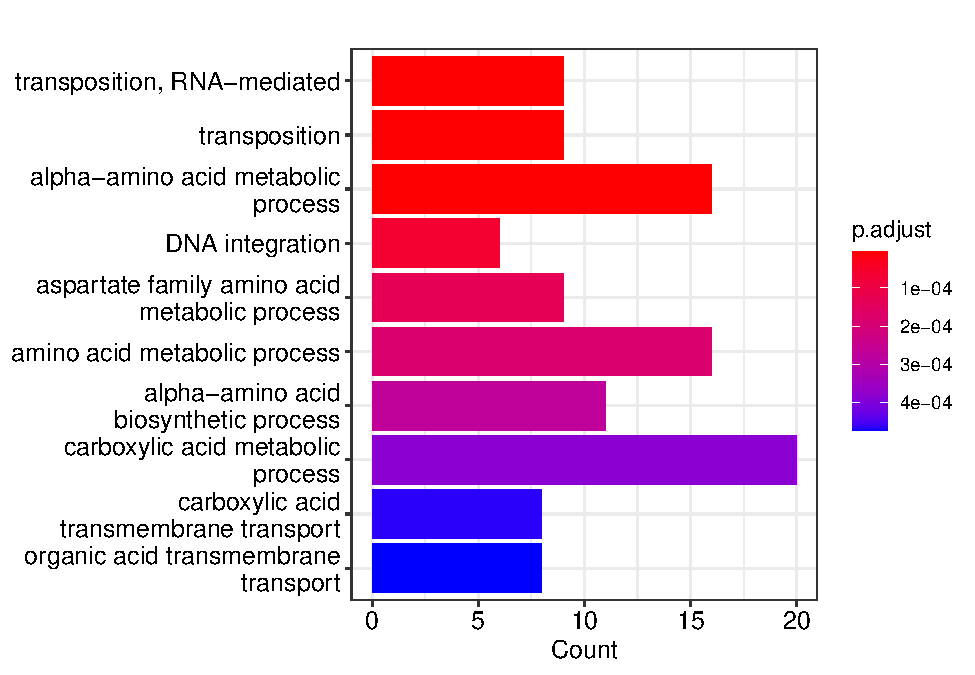
\includegraphics{_main_files/figure-latex/visualize-GOterms_upregulated_phenol-GO-1.pdf}

\begin{Shaded}
\begin{Highlighting}[]
\CommentTok{\# a more complicated visualization, with more information density}
\FunctionTok{ggplot}\NormalTok{(GO\_msn24\_EtOH\_up\_results,}
       \AttributeTok{showCategory =} \DecValTok{15}\NormalTok{,}
       \FunctionTok{aes}\NormalTok{(richFactor, }\FunctionTok{fct\_reorder}\NormalTok{(Description, richFactor))) }\SpecialCharTok{+}
  \FunctionTok{geom\_segment}\NormalTok{(}\FunctionTok{aes}\NormalTok{(}\AttributeTok{xend =} \DecValTok{0}\NormalTok{, }\AttributeTok{yend =}\NormalTok{ Description)) }\SpecialCharTok{+}
  \FunctionTok{geom\_point}\NormalTok{(}\FunctionTok{aes}\NormalTok{(}\AttributeTok{color =}\NormalTok{ p.adjust, }\AttributeTok{size =}\NormalTok{ Count)) }\SpecialCharTok{+}
  \FunctionTok{scale\_color\_gradientn}\NormalTok{(}
    \AttributeTok{colours =} \FunctionTok{c}\NormalTok{(}\StringTok{"\#f7ca64"}\NormalTok{, }\StringTok{"\#46bac2"}\NormalTok{, }\StringTok{"\#7e62a3"}\NormalTok{),}
    \AttributeTok{trans =} \StringTok{"log10"}\NormalTok{,}
    \AttributeTok{guide =} \FunctionTok{guide\_colorbar}\NormalTok{(}\AttributeTok{reverse =} \ConstantTok{TRUE}\NormalTok{, }\AttributeTok{order =} \DecValTok{1}\NormalTok{)}
\NormalTok{  ) }\SpecialCharTok{+}
  \FunctionTok{scale\_size\_continuous}\NormalTok{(}\AttributeTok{range =} \FunctionTok{c}\NormalTok{(}\DecValTok{2}\NormalTok{, }\DecValTok{10}\NormalTok{)) }\SpecialCharTok{+}
  \FunctionTok{xlab}\NormalTok{(}\StringTok{"Rich Factor"}\NormalTok{) }\SpecialCharTok{+}
  \FunctionTok{ylab}\NormalTok{(}\ConstantTok{NULL}\NormalTok{) }\SpecialCharTok{+}
  \FunctionTok{ggtitle}\NormalTok{(}\StringTok{"Biological Processes"}\NormalTok{) }\SpecialCharTok{+}
  \FunctionTok{theme\_bw}\NormalTok{()}
\end{Highlighting}
\end{Shaded}

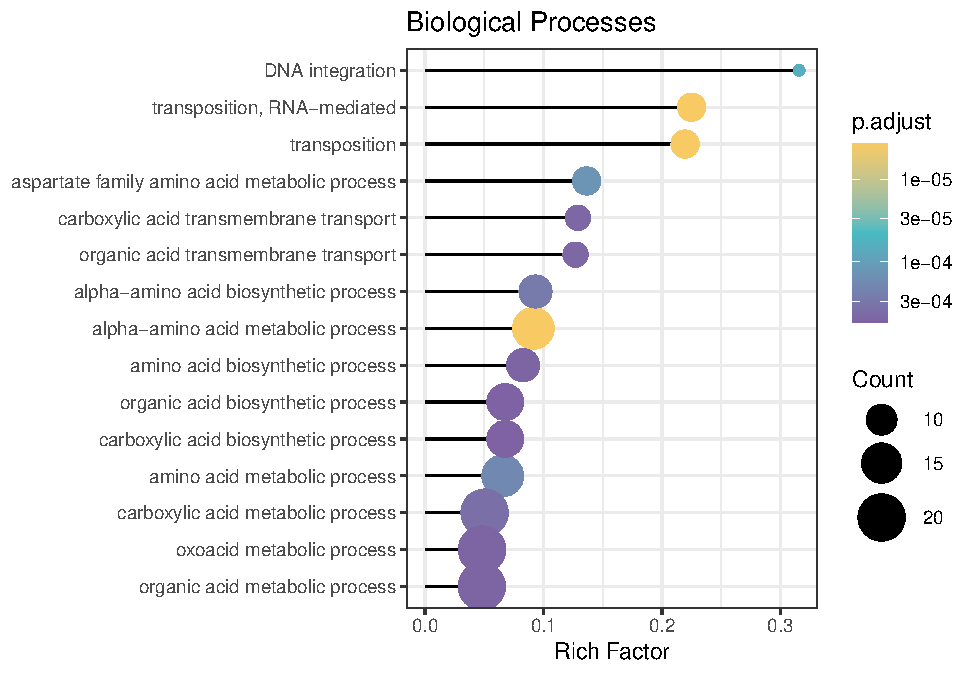
\includegraphics{_main_files/figure-latex/visualize-GOterms_upregulated_phenol-GO-2.pdf}

You can try adjusting the size of the output figures by clicking the gear icon in the top right of the code chunk and click ``use custom figure size''. Note this updates the chunk header so the change is saved.

\hypertarget{saving-ggplot-output-to-a-file}{%
\subsection{Saving ggplot output to a file}\label{saving-ggplot-output-to-a-file}}

We usually want to save our visualizations for later. When plotting with the ggplot package, there is an easy way to do this. See below:

\begin{Shaded}
\begin{Highlighting}[]
\CommentTok{\# First, let\textquotesingle{}s create a folder to save our visualizations}
\NormalTok{dir\_visualization }\OtherTok{\textless{}{-}} \FunctionTok{path.expand}\NormalTok{(}\StringTok{"\textasciitilde{}/Desktop/Genomic\_Data\_Analysis/Visualization/"}\NormalTok{)}
\ControlFlowTok{if}\NormalTok{ (}\SpecialCharTok{!}\FunctionTok{dir.exists}\NormalTok{(dir\_visualization)) \{}\FunctionTok{dir.create}\NormalTok{(dir\_visualization, }\AttributeTok{recursive =} \ConstantTok{TRUE}\NormalTok{)\}}

\CommentTok{\# type ?ggsave in the console for more information via the help page.}
\FunctionTok{ggsave}\NormalTok{(}
  \StringTok{"GO\_BP\_msn24\_EtOH\_up\_results\_lollipopPlot.pdf"}\NormalTok{, }
  \CommentTok{\# if we don\textquotesingle{}t need the image to go to a certain spot, we only need the file name above.}
  \AttributeTok{plot =} \FunctionTok{last\_plot}\NormalTok{(), }\CommentTok{\# either the last plot, or name of a ggplot object you\textquotesingle{}ve saved.}
  \AttributeTok{device =} \StringTok{"pdf"}\NormalTok{, }\CommentTok{\#Can be "png", "eps", "ps", "tex" (pictex), "pdf", "jpeg", "tiff", "png", "bmp", "svg" or "wmf" (windows only).}
  \CommentTok{\# note that pdf, eps, svg are vector/line art, so zooming doesn\textquotesingle{}t pixelate.}
  \AttributeTok{path =}\NormalTok{ dir\_visualization, }\CommentTok{\# Path of the directory to save plot to. defaults to work dir.}
  \AttributeTok{scale =} \DecValTok{2}\NormalTok{, }\CommentTok{\# multiplicative scaling factor }
  \AttributeTok{width =} \DecValTok{12}\NormalTok{,}
  \AttributeTok{height =} \DecValTok{8}\NormalTok{,}
  \AttributeTok{units =} \StringTok{"cm"}\NormalTok{, }\CommentTok{\# must be one of: "in", "cm", "mm", "px"}
  \AttributeTok{dpi =} \DecValTok{300}\NormalTok{,  }\CommentTok{\# adjusting this larger gives higher quality plot, making a larger file.}
  \AttributeTok{limitsize =} \ConstantTok{TRUE}\NormalTok{, }\CommentTok{\# prevents accidentally making it massive, defaults to TRUE}
  \AttributeTok{bg =} \ConstantTok{NULL} \CommentTok{\# Background colour. If NULL, uses the plot.background fill value from the plot theme.}
\NormalTok{)}
\end{Highlighting}
\end{Shaded}

Recall that when we knit this Rmarkdown notebook, we keep a copy of the plots/images there as well, in the same place as the code and analysis used to generate it. However, we may want a higher resolution file of just the image, or the image in a different format. In this case, saving the plot is a useful option for us. The journal Science has the following \href{https://www.science.org/do/10.5555/page.2385607/full/author_figure_prep_guide_2022-1689707679870.pdf}{recommendations}: ``We prefer prefer ai, eps, pdf, layered psd, tif, and jpeg files. \ldots minimum file resolution of 300 dpi.''

\hypertarget{the-hypergeometric-distribution-in-practice}{%
\section{The Hypergeometric Distribution in practice}\label{the-hypergeometric-distribution-in-practice}}

Notice that the DNA integration process does not have very many genes in the category, but they appear to be highly present in the the upregulated gene list. Specifically, DE genes have this GO term, where in the entire genome, there are only genes. What are the odds that we see this by random chance? let's do the math:

\begin{Shaded}
\begin{Highlighting}[]
\CommentTok{\# number of genes that have GO:0015074 (DNA integration)}
\NormalTok{integration\_genes }\OtherTok{=} \DecValTok{23}
\CommentTok{\# number of genes that are DE (msn2/4 EtOH response, logFC\textgreater{}1)}
\NormalTok{DE\_genes }\OtherTok{=} \DecValTok{91}
\CommentTok{\# number of genes that are both DE and DNA integration genes}
\NormalTok{Overlap }\OtherTok{=} \DecValTok{6}
\CommentTok{\# total number of genes in experiment}
\NormalTok{total }\OtherTok{=} \DecValTok{5538} \CommentTok{\# number of genes in genome}
\end{Highlighting}
\end{Shaded}

\textbf{Without doing the math, do you expect these to be underrepresented, overrepresented, or neither?}

\begin{Shaded}
\begin{Highlighting}[]
\CommentTok{\# test for underrepresentation (depletion)}
\FunctionTok{phyper}\NormalTok{(}\AttributeTok{q =}\NormalTok{ Overlap, }\CommentTok{\# number of integration genes that were DE}
       \AttributeTok{m =}\NormalTok{ DE\_genes, }\CommentTok{\# number of DE genes}
       \AttributeTok{n =}\NormalTok{ total}\SpecialCharTok{{-}}\NormalTok{DE\_genes, }\CommentTok{\# number of non DE genes}
       \AttributeTok{k =}\NormalTok{ integration\_genes, }\CommentTok{\# number of observed DE DNA integration genes}
       \AttributeTok{lower.tail =} \ConstantTok{TRUE}\NormalTok{) }\CommentTok{\# the probability that X \textless{}= x}
\end{Highlighting}
\end{Shaded}

\begin{verbatim}
## [1] 0.9999999
\end{verbatim}

\begin{Shaded}
\begin{Highlighting}[]
\CommentTok{\# test for overrepresentation (enrichmen t)}
\FunctionTok{phyper}\NormalTok{(}\AttributeTok{q =}\NormalTok{ Overlap}\DecValTok{{-}1}\NormalTok{, }\CommentTok{\# number of integration genes that were DE}
                      \CommentTok{\# we subtract 1 b/c of lower.tail=FALSE means greater than}
                      \CommentTok{\# without equality, so have to do one less}
       \AttributeTok{m =}\NormalTok{ DE\_genes, }\CommentTok{\# number of DE genes}
       \AttributeTok{n =}\NormalTok{ total}\SpecialCharTok{{-}}\NormalTok{DE\_genes, }\CommentTok{\# number of non DE genes}
       \AttributeTok{k =}\NormalTok{ integration\_genes, }\CommentTok{\# number of observed DE integration genes}
       \AttributeTok{lower.tail =} \ConstantTok{FALSE}\NormalTok{) }\CommentTok{\# the probability that X \textgreater{} x}
\end{Highlighting}
\end{Shaded}

\begin{verbatim}
## [1] 1.344447e-06
\end{verbatim}

As we see, there is strong evidence that the number of genes with this GO term is unlikely to be seen due to chance. In layman's terms, this GO term is enriched in upregulated genes in this contrast. The test for underrepresenation shows there is no support for a hypothesis that this gene is underrepresented in the DE gene list.

Interestingly, the hypergeometric distribution is the same thing as the Fisher's Exact test, so we can rerun the same tests above with a different command:

\begin{Shaded}
\begin{Highlighting}[]
\CommentTok{\#fisher test for underrepresentation}
\FunctionTok{fisher.test}\NormalTok{(}\FunctionTok{matrix}\NormalTok{(}\FunctionTok{c}\NormalTok{(Overlap, DE\_genes}\SpecialCharTok{{-}}\NormalTok{Overlap, integration\_genes}\SpecialCharTok{{-}}\NormalTok{Overlap, total}\SpecialCharTok{{-}}\NormalTok{DE\_genes}\SpecialCharTok{{-}}\NormalTok{integration\_genes }\SpecialCharTok{+}\NormalTok{ Overlap), }\DecValTok{2}\NormalTok{, }\DecValTok{2}\NormalTok{), }\AttributeTok{alternative=}\StringTok{\textquotesingle{}less\textquotesingle{}}\NormalTok{)}\SpecialCharTok{$}\NormalTok{p.value}
\end{Highlighting}
\end{Shaded}

\begin{verbatim}
## [1] 0.9999999
\end{verbatim}

\begin{Shaded}
\begin{Highlighting}[]
\CommentTok{\#fisher test for overrepresentation}
\FunctionTok{fisher.test}\NormalTok{(}\FunctionTok{matrix}\NormalTok{(}\FunctionTok{c}\NormalTok{(Overlap, DE\_genes}\SpecialCharTok{{-}}\NormalTok{Overlap, integration\_genes}\SpecialCharTok{{-}}\NormalTok{Overlap, total}\SpecialCharTok{{-}}\NormalTok{DE\_genes}\SpecialCharTok{{-}}\NormalTok{integration\_genes }\SpecialCharTok{+}\NormalTok{ Overlap), }\DecValTok{2}\NormalTok{, }\DecValTok{2}\NormalTok{), }\AttributeTok{alternative=}\StringTok{\textquotesingle{}greater\textquotesingle{}}\NormalTok{)}\SpecialCharTok{$}\NormalTok{p.value}
\end{Highlighting}
\end{Shaded}

\begin{verbatim}
## [1] 1.344447e-06
\end{verbatim}

How does the p-value that we get from this test compare to the results table? They should match.

\hypertarget{now-it-is-your-turn}{%
\section{Now it is your turn}\label{now-it-is-your-turn}}

Try running your own GO enrichment with a different gene list. Some options could be:

\begin{itemize}
\tightlist
\item
  Start with the WT vs \emph{msn2/4ΔΔ}: EtOH response again, and this time change to ``downregulated'' (i.e., genes with higher expression in the wild-type strain compared to the \emph{msn2/4ΔΔ} mutant). These would potentially include genes with defective induction.
\item
  See what happens when you change the FDR threshold from a liberal one (0.05) to a more conservative one (0.01).
\item
  Try different logFC cutoffs.
\item
  Look at different comparisons in the data file (there are 5 total)
\item
  Look at a different GO category (we only looked at BP, not MF or CC)
\item
  Advanced: include multiple filters (e.g., genes upregulated by EtOH stress in the WT strain that ALSO have defective induction during ethanol stress in the \emph{msn2/4ΔΔ} mutant).
\end{itemize}

The code below is a template for you to modify to complete this activity. The example code below looks at the downregulated genes in response to stress in the WT (choose something else for your gene list)

\begin{center}\rule{0.5\linewidth}{0.5pt}\end{center}

\begin{Shaded}
\begin{Highlighting}[]
\CommentTok{\# subset to just genes meeting your requirements}
\NormalTok{DE\_genes\_GIVE\_NAME }\OtherTok{\textless{}{-}}\NormalTok{ msn24\_EtOH }\SpecialCharTok{|\textgreater{}}
  \CommentTok{\# change the below line for the filters that you want}
  \FunctionTok{filter}\NormalTok{(log\_fc\_yps606\_wt\_et\_oh\_response }\SpecialCharTok{\textless{}} \DecValTok{1} \SpecialCharTok{\&}\NormalTok{ pvalue\_yps606\_wt\_et\_oh\_response}\SpecialCharTok{\textless{}}\FloatTok{0.05}\NormalTok{) }\SpecialCharTok{|\textgreater{}} 
  \FunctionTok{pull}\NormalTok{(gene\_id) }\CommentTok{\# grabbing just the gene names}
\end{Highlighting}
\end{Shaded}

\hypertarget{run-enrichment}{%
\subsection{Run Enrichment}\label{run-enrichment}}

\begin{Shaded}
\begin{Highlighting}[]
\NormalTok{GO\_GIVE\_NAME\_results }\OtherTok{\textless{}{-}} \FunctionTok{enrichGO}\NormalTok{(}
  \AttributeTok{gene =}\NormalTok{ DE\_genes\_GIVE\_NAME,}
  \AttributeTok{OrgDb =} \StringTok{"org.Sc.sgd.db"}\NormalTok{,}
  \AttributeTok{universe =}\NormalTok{ msn24\_EtOH}\SpecialCharTok{$}\NormalTok{gene\_id,}
  \AttributeTok{keyType =} \StringTok{"ORF"}\NormalTok{,}
  \AttributeTok{ont=} \StringTok{"BP"}
\NormalTok{) }\SpecialCharTok{|\textgreater{}}
  \FunctionTok{mutate}\NormalTok{(}\AttributeTok{richFactor =}\NormalTok{ Count }\SpecialCharTok{/} \FunctionTok{as.numeric}\NormalTok{(}\FunctionTok{sub}\NormalTok{(}\StringTok{"/}\SpecialCharTok{\textbackslash{}\textbackslash{}}\StringTok{d+"}\NormalTok{, }\StringTok{""}\NormalTok{, BgRatio)))}
\end{Highlighting}
\end{Shaded}

\hypertarget{see-the-data}{%
\subsection{see the data}\label{see-the-data}}

\begin{Shaded}
\begin{Highlighting}[]
\CommentTok{\# open up the results in a data frame to examine}
\NormalTok{GO\_GIVE\_NAME\_results }\SpecialCharTok{|\textgreater{}}
  \FunctionTok{as\_tibble}\NormalTok{() }\SpecialCharTok{|\textgreater{}}
  \FunctionTok{View}\NormalTok{()}

\CommentTok{\# write out your results to a text file}
\NormalTok{GO\_GIVE\_NAME\_results }\SpecialCharTok{|\textgreater{}}
  \FunctionTok{as\_tibble}\NormalTok{() }\SpecialCharTok{|\textgreater{}}
  \FunctionTok{write\_tsv}\NormalTok{(}\AttributeTok{file =} \StringTok{"\textasciitilde{}/Desktop/GO\_GIVE\_NAME\_DIRECTION\_results.tsv"}\NormalTok{)}
\end{Highlighting}
\end{Shaded}

\hypertarget{create-plots}{%
\subsection{create plots}\label{create-plots}}

\begin{Shaded}
\begin{Highlighting}[]
\CommentTok{\# a simple visualization}
\FunctionTok{plot}\NormalTok{(}\FunctionTok{barplot}\NormalTok{(GO\_GIVE\_NAME\_results, }\AttributeTok{showCategory =} \DecValTok{10}\NormalTok{))}
\end{Highlighting}
\end{Shaded}

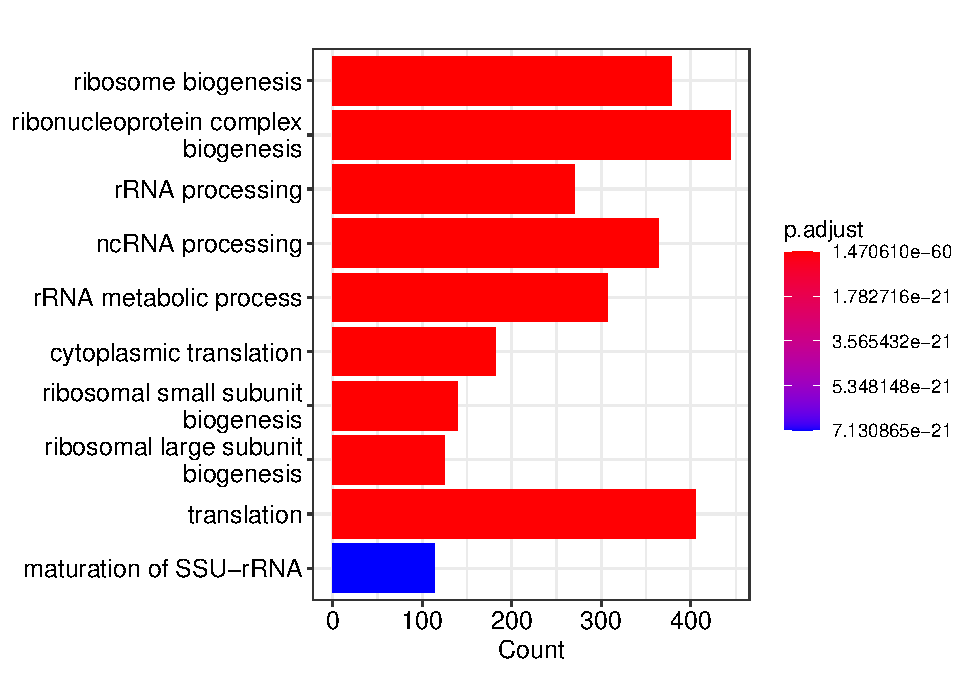
\includegraphics{_main_files/figure-latex/visualize-GOterms_(direction)(treatment)-GO-1.pdf}

\begin{Shaded}
\begin{Highlighting}[]
\CommentTok{\# built in visualization with dots instead}
\FunctionTok{dotplot}\NormalTok{(GO\_GIVE\_NAME\_results, }\AttributeTok{showCategory=}\DecValTok{10}\NormalTok{) }
\end{Highlighting}
\end{Shaded}

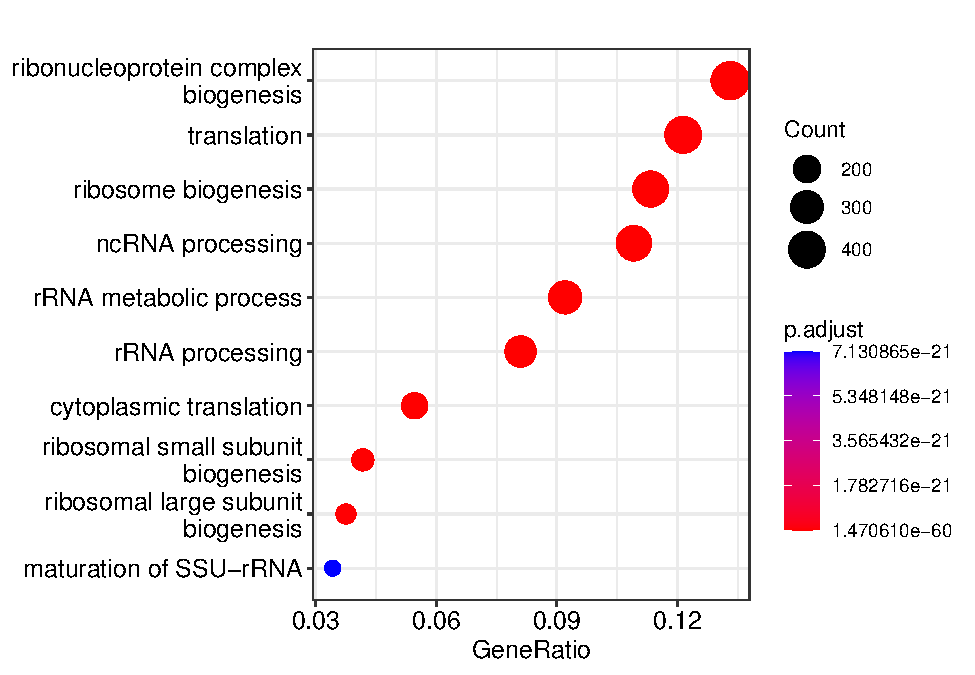
\includegraphics{_main_files/figure-latex/visualize-GOterms_(direction)(treatment)-GO-2.pdf}

\begin{Shaded}
\begin{Highlighting}[]
\CommentTok{\# a more complicated visualization, with more information density}
\FunctionTok{ggplot}\NormalTok{(GO\_GIVE\_NAME\_results,}
       \AttributeTok{showCategory =} \DecValTok{15}\NormalTok{,}
       \FunctionTok{aes}\NormalTok{(richFactor, }\FunctionTok{fct\_reorder}\NormalTok{(Description, richFactor))) }\SpecialCharTok{+}
  \FunctionTok{geom\_segment}\NormalTok{(}\FunctionTok{aes}\NormalTok{(}\AttributeTok{xend =} \DecValTok{0}\NormalTok{, }\AttributeTok{yend =}\NormalTok{ Description)) }\SpecialCharTok{+}
  \FunctionTok{geom\_point}\NormalTok{(}\FunctionTok{aes}\NormalTok{(}\AttributeTok{color =}\NormalTok{ p.adjust, }\AttributeTok{size =}\NormalTok{ Count)) }\SpecialCharTok{+}
  \FunctionTok{scale\_color\_gradientn}\NormalTok{(}
    \AttributeTok{colours =} \FunctionTok{c}\NormalTok{(}\StringTok{"\#f7ca64"}\NormalTok{, }\StringTok{"\#46bac2"}\NormalTok{, }\StringTok{"\#7e62a3"}\NormalTok{),}
    \AttributeTok{trans =} \StringTok{"log10"}\NormalTok{,}
    \AttributeTok{guide =} \FunctionTok{guide\_colorbar}\NormalTok{(}\AttributeTok{reverse =} \ConstantTok{TRUE}\NormalTok{, }\AttributeTok{order =} \DecValTok{1}\NormalTok{)}
\NormalTok{  ) }\SpecialCharTok{+}
  \FunctionTok{scale\_size\_continuous}\NormalTok{(}\AttributeTok{range =} \FunctionTok{c}\NormalTok{(}\DecValTok{2}\NormalTok{, }\DecValTok{10}\NormalTok{)) }\SpecialCharTok{+}
  \FunctionTok{scale\_y\_discrete}\NormalTok{(}\AttributeTok{label =} \ControlFlowTok{function}\NormalTok{(x) stringr}\SpecialCharTok{::}\FunctionTok{str\_trunc}\NormalTok{(x, }\DecValTok{50}\NormalTok{)) }\SpecialCharTok{+} \CommentTok{\# cut off long names}
  \FunctionTok{xlab}\NormalTok{(}\StringTok{"Rich Factor"}\NormalTok{) }\SpecialCharTok{+}
  \FunctionTok{ylab}\NormalTok{(}\ConstantTok{NULL}\NormalTok{) }\SpecialCharTok{+}
  \FunctionTok{ggtitle}\NormalTok{(}\StringTok{"Biological Processes"}\NormalTok{) }\SpecialCharTok{+}
  \FunctionTok{theme\_bw}\NormalTok{()}
\end{Highlighting}
\end{Shaded}

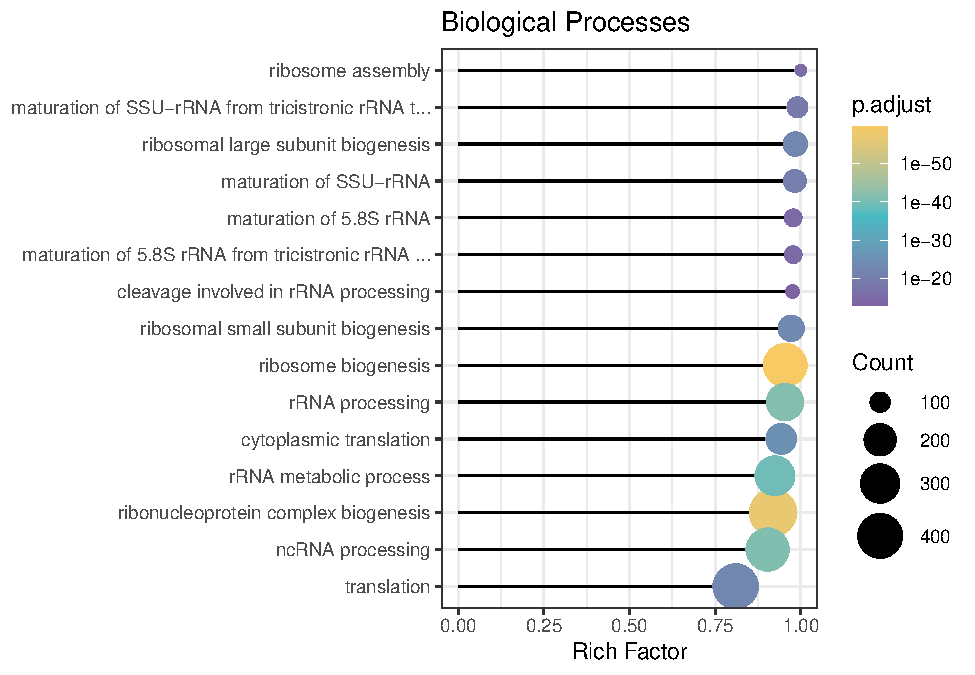
\includegraphics{_main_files/figure-latex/visualize-GOterms_(direction)(treatment)-GO-3.pdf}

\hypertarget{questions}{%
\section{Questions}\label{questions}}

Answer the following questions:

\begin{enumerate}
\def\labelenumi{\arabic{enumi}.}
\item
  Which GO term had the smallest adjusted p-value in the upregulated comparison example that we did together?
\item
  What percent of the genes would we expect to have that GO term in the DE list under the null hypothesis? What percent of the DE genes actually had that GO term?
\item
  For the upregulated comparision, what GO terms are enriched for genes with pval \textless{} 0.01 but fdr \textgreater{} 0.01 and what is their average/median log fold change?
\item
  For one of your own novel comparisons, explain what comparison you were interested in, and your rationale for the cutoffs you chose for your gene list.
\item
  For that novel gene list you chose for yourself, which GO term had the smallest adjusted p-value?
\item
  In simple terms, how would you describe what the ``Rich Factor'' tells about a given GO term in the gene list.
\item
  Challenge: create a venn diagram of the GO terms in the GO analysis you ran comparing to the upregulated comparison example.
\end{enumerate}

\begin{Shaded}
\begin{Highlighting}[]
\CommentTok{\# create a list of the data we want to compare}
\NormalTok{GO\_results\_list }\OtherTok{\textless{}{-}} \FunctionTok{list}\NormalTok{(}\FunctionTok{data.frame}\NormalTok{(GO\_msn24\_EtOH\_up\_results)}\SpecialCharTok{$}\NormalTok{ID,}
                        \FunctionTok{data.frame}\NormalTok{(GO\_GIVE\_NAME\_results)}\SpecialCharTok{$}\NormalTok{ID)}

\CommentTok{\# visualize the GO results list as a venn diagram}
\FunctionTok{ggVennDiagram}\NormalTok{(GO\_results\_list,}
              \AttributeTok{category.names =} \FunctionTok{c}\NormalTok{(}\StringTok{"msn24\_EtOH\_upregulated"}\NormalTok{, }\StringTok{"[GIVE\_NAME]"}\NormalTok{)) }\SpecialCharTok{+}
  \FunctionTok{scale\_x\_continuous}\NormalTok{(}\AttributeTok{expand =} \FunctionTok{expansion}\NormalTok{(}\AttributeTok{mult =}\NormalTok{ .}\DecValTok{2}\NormalTok{)) }\SpecialCharTok{+}
  \FunctionTok{scale\_fill\_distiller}\NormalTok{(}\AttributeTok{palette =} \StringTok{"RdBu"}
\NormalTok{  )}
\end{Highlighting}
\end{Shaded}

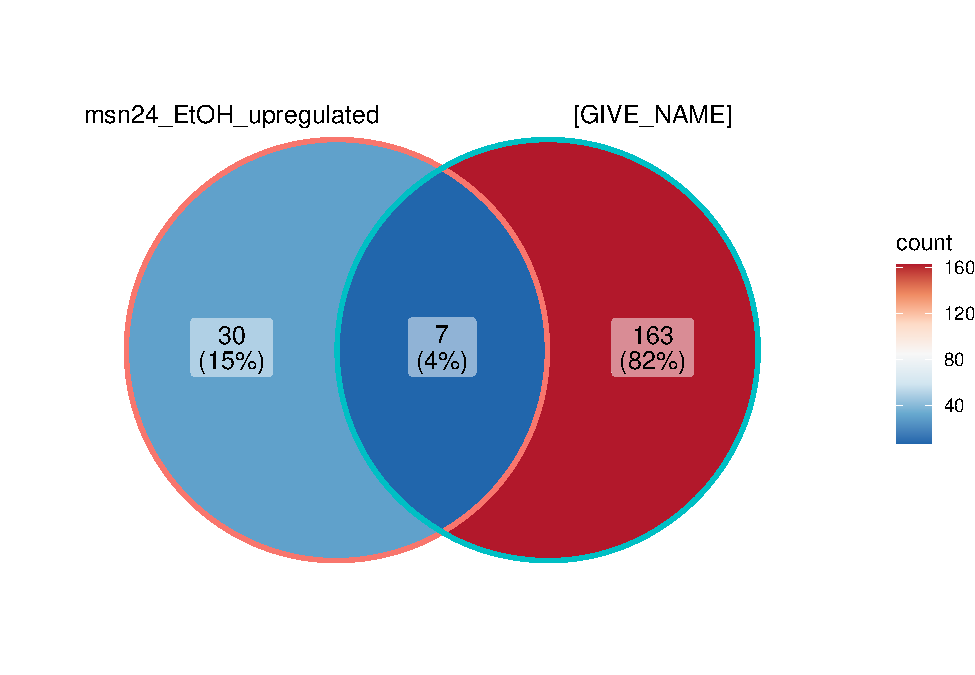
\includegraphics{_main_files/figure-latex/create-vennDiagram-1.pdf}

Be sure to knit this file into a pdf or html file once you're finished.

System information for reproducibility:

\begin{Shaded}
\begin{Highlighting}[]
\NormalTok{pander}\SpecialCharTok{::}\FunctionTok{pander}\NormalTok{(}\FunctionTok{sessionInfo}\NormalTok{())}
\end{Highlighting}
\end{Shaded}

\textbf{R version 4.3.1 (2023-06-16)}

\textbf{Platform:} aarch64-apple-darwin20 (64-bit)

\textbf{locale:}
en\_US.UTF-8\textbar\textbar en\_US.UTF-8\textbar\textbar en\_US.UTF-8\textbar\textbar C\textbar\textbar en\_US.UTF-8\textbar\textbar en\_US.UTF-8

\textbf{attached base packages:}
\emph{stats4}, \emph{stats}, \emph{graphics}, \emph{grDevices}, \emph{utils}, \emph{datasets}, \emph{methods} and \emph{base}

\textbf{other attached packages:}
\emph{org.Sc.sgd.db(v.3.17.0)}, \emph{AnnotationDbi(v.1.62.2)}, \emph{IRanges(v.2.34.1)}, \emph{S4Vectors(v.0.38.2)}, \emph{Biobase(v.2.60.0)}, \emph{BiocGenerics(v.0.46.0)}, \emph{clusterProfiler(v.4.8.2)}, \emph{ggVennDiagram(v.1.2.3)}, \emph{tidytree(v.0.4.5)}, \emph{igraph(v.1.5.1)}, \emph{janitor(v.2.2.0)}, \emph{BiocManager(v.1.30.22)}, \emph{pander(v.0.6.5)}, \emph{knitr(v.1.44)}, \emph{here(v.1.0.1)}, \emph{lubridate(v.1.9.3)}, \emph{forcats(v.1.0.0)}, \emph{stringr(v.1.5.0)}, \emph{dplyr(v.1.1.3)}, \emph{purrr(v.1.0.2)}, \emph{readr(v.2.1.4)}, \emph{tidyr(v.1.3.0)}, \emph{tibble(v.3.2.1)}, \emph{ggplot2(v.3.4.4)}, \emph{tidyverse(v.2.0.0)} and \emph{pacman(v.0.5.1)}

\textbf{loaded via a namespace (and not attached):}
\emph{RColorBrewer(v.1.1-3)}, \emph{rstudioapi(v.0.15.0)}, \emph{jsonlite(v.1.8.7)}, \emph{magrittr(v.2.0.3)}, \emph{farver(v.2.1.1)}, \emph{rmarkdown(v.2.25)}, \emph{ragg(v.1.2.6)}, \emph{fs(v.1.6.3)}, \emph{zlibbioc(v.1.46.0)}, \emph{vctrs(v.0.6.4)}, \emph{memoise(v.2.0.1)}, \emph{RCurl(v.1.98-1.12)}, \emph{ggtree(v.3.8.2)}, \emph{htmltools(v.0.5.6.1)}, \emph{curl(v.5.1.0)}, \emph{gridGraphics(v.0.5-1)}, \emph{KernSmooth(v.2.23-22)}, \emph{plyr(v.1.8.9)}, \emph{cachem(v.1.0.8)}, \emph{lifecycle(v.1.0.3)}, \emph{pkgconfig(v.2.0.3)}, \emph{Matrix(v.1.6-1.1)}, \emph{R6(v.2.5.1)}, \emph{fastmap(v.1.1.1)}, \emph{gson(v.0.1.0)}, \emph{GenomeInfoDbData(v.1.2.10)}, \emph{snakecase(v.0.11.1)}, \emph{digest(v.0.6.33)}, \emph{aplot(v.0.2.2)}, \emph{enrichplot(v.1.20.0)}, \emph{colorspace(v.2.1-0)}, \emph{patchwork(v.1.1.3)}, \emph{rprojroot(v.2.0.3)}, \emph{textshaping(v.0.3.7)}, \emph{RSQLite(v.2.3.1)}, \emph{labeling(v.0.4.3)}, \emph{fansi(v.1.0.5)}, \emph{timechange(v.0.2.0)}, \emph{httr(v.1.4.7)}, \emph{polyclip(v.1.10-6)}, \emph{compiler(v.4.3.1)}, \emph{proxy(v.0.4-27)}, \emph{bit64(v.4.0.5)}, \emph{withr(v.2.5.1)}, \emph{downloader(v.0.4)}, \emph{BiocParallel(v.1.34.2)}, \emph{viridis(v.0.6.4)}, \emph{DBI(v.1.1.3)}, \emph{ggforce(v.0.4.1)}, \emph{MASS(v.7.3-60)}, \emph{classInt(v.0.4-10)}, \emph{HDO.db(v.0.99.1)}, \emph{units(v.0.8-4)}, \emph{tools(v.4.3.1)}, \emph{ape(v.5.7-1)}, \emph{scatterpie(v.0.2.1)}, \emph{glue(v.1.6.2)}, \emph{nlme(v.3.1-163)}, \emph{GOSemSim(v.2.26.1)}, \emph{sf(v.1.0-14)}, \emph{grid(v.4.3.1)}, \emph{shadowtext(v.0.1.2)}, \emph{reshape2(v.1.4.4)}, \emph{fgsea(v.1.26.0)}, \emph{generics(v.0.1.3)}, \emph{gtable(v.0.3.4)}, \emph{tzdb(v.0.4.0)}, \emph{class(v.7.3-22)}, \emph{data.table(v.1.14.8)}, \emph{hms(v.1.1.3)}, \emph{tidygraph(v.1.2.3)}, \emph{utf8(v.1.2.3)}, \emph{XVector(v.0.40.0)}, \emph{ggrepel(v.0.9.4)}, \emph{pillar(v.1.9.0)}, \emph{yulab.utils(v.0.1.0)}, \emph{vroom(v.1.6.4)}, \emph{splines(v.4.3.1)}, \emph{tweenr(v.2.0.2)}, \emph{treeio(v.1.24.3)}, \emph{lattice(v.0.21-9)}, \emph{bit(v.4.0.5)}, \emph{tidyselect(v.1.2.0)}, \emph{GO.db(v.3.17.0)}, \emph{Biostrings(v.2.68.1)}, \emph{gridExtra(v.2.3)}, \emph{bookdown(v.0.36)}, \emph{xfun(v.0.40)}, \emph{graphlayouts(v.1.0.1)}, \emph{stringi(v.1.7.12)}, \emph{lazyeval(v.0.2.2)}, \emph{ggfun(v.0.1.3)}, \emph{yaml(v.2.3.7)}, \emph{evaluate(v.0.22)}, \emph{codetools(v.0.2-19)}, \emph{ggraph(v.2.1.0)}, \emph{qvalue(v.2.32.0)}, \emph{RVenn(v.1.1.0)}, \emph{ggplotify(v.0.1.2)}, \emph{cli(v.3.6.1)}, \emph{systemfonts(v.1.0.5)}, \emph{munsell(v.0.5.0)}, \emph{Rcpp(v.1.0.11)}, \emph{GenomeInfoDb(v.1.36.4)}, \emph{png(v.0.1-8)}, \emph{parallel(v.4.3.1)}, \emph{blob(v.1.2.4)}, \emph{DOSE(v.3.26.1)}, \emph{bitops(v.1.0-7)}, \emph{viridisLite(v.0.4.2)}, \emph{e1071(v.1.7-13)}, \emph{scales(v.1.2.1)}, \emph{crayon(v.1.5.2)}, \emph{rlang(v.1.1.1)}, \emph{cowplot(v.1.1.1)}, \emph{fastmatch(v.1.1-4)} and \emph{KEGGREST(v.1.40.1)}

\hypertarget{working-with-sequences-raw-data-quality-control}{%
\chapter{Working with Sequences: Raw Data \& Quality Control}\label{working-with-sequences-raw-data-quality-control}}

last updated: 2023-10-26

\hypertarget{package-install}{%
\section{Package Install}\label{package-install}}

As usual, make sure we have the right packages for this exercise

\begin{Shaded}
\begin{Highlighting}[]
\ControlFlowTok{if}\NormalTok{ (}\SpecialCharTok{!}\FunctionTok{require}\NormalTok{(}\StringTok{"pacman"}\NormalTok{)) }\FunctionTok{install.packages}\NormalTok{(}\StringTok{"pacman"}\NormalTok{); }\FunctionTok{library}\NormalTok{(pacman)}

\CommentTok{\# let\textquotesingle{}s load all of the files we were using and want to have again today}
\FunctionTok{p\_load}\NormalTok{(}\StringTok{"tidyverse"}\NormalTok{, }\StringTok{"knitr"}\NormalTok{, }\StringTok{"readr"}\NormalTok{,}
       \StringTok{"pander"}\NormalTok{, }\StringTok{"BiocManager"}\NormalTok{, }
       \StringTok{"dplyr"}\NormalTok{, }\StringTok{"stringr"}\NormalTok{)}

\CommentTok{\# We also need the bioconductor packages "ShortRead" and "rfastp" for today\textquotesingle{}s activity.}
\FunctionTok{p\_load}\NormalTok{(}\StringTok{"Rfastp"}\NormalTok{, }\StringTok{"ShortRead"}\NormalTok{)}
\end{Highlighting}
\end{Shaded}

\hypertarget{description-1}{%
\section{Description}\label{description-1}}

This activity is intended to familiarize you with raw bioinformatic sequence files. Specifically, we'll be working with short read sequencing data generated from an Illumina platform.

\hypertarget{learning-outcomes-2}{%
\section{Learning outcomes}\label{learning-outcomes-2}}

At the end of this exercise, you should be able to:

\begin{itemize}
\tightlist
\item
  Load and read into R a raw gzipped fastq file.
\item
  Inspect sequence quality and evaluate results.
\item
  Perform quality control on raw data and save the processed output.
\end{itemize}

Note that instead of \texttt{\{r\}}, the below chunk uses \texttt{\{bash\}}, meaning this isn't r code but bash code (the language used in the terminal). The \texttt{-nc} flag ensures the files are only downloaded if they don't already exist where you are downloading them.

This may take awhile the first time you run it. The below script is a bash command that downloads these files to your computer

\hypertarget{download-fastq}{%
\section{Download fastq}\label{download-fastq}}

\begin{Shaded}
\begin{Highlighting}[]
\CommentTok{\# Be sure to change this file path to the path you want your data to go}
\VariableTok{RAW\_DATA\_DIR}\OperatorTok{=}\StringTok{"/Users/}\VariableTok{$USER}\StringTok{/Desktop/Genomic\_Data\_Analysis/Data/Raw"}

\CommentTok{\#if you\textquotesingle{}re using Windows 10,}
\CommentTok{\# in RStudio, go to Tools\textgreater{}Global Options... \textgreater{} Terminal \textgreater{} New Terminals open with...}
\CommentTok{\# and choose WSL bash or git bash}
\CommentTok{\# next, use: (be sure to put in the correct username)}
\CommentTok{\#RAW\_DATA\_DIR="/mnt/c/Users/$USER/Desktop/Genomic\_Data\_Analysis/Data/Raw"}

\CommentTok{\# create the destination directory if it doesn\textquotesingle{}t already exist}
\FunctionTok{mkdir} \AttributeTok{{-}p} \VariableTok{$RAW\_DATA\_DIR}

\BuiltInTok{echo} \VariableTok{$RAW\_DATA\_DIR}

\CommentTok{\# change to that directory (for this code chunk only)}
\BuiltInTok{cd} \VariableTok{$RAW\_DATA\_DIR}
\BuiltInTok{pwd}
\CommentTok{\# Download the files.}
\CommentTok{\# }\AlertTok{WARNING}\CommentTok{: curl doesn\textquotesingle{}t work with relative paths}
\CommentTok{\# WT unstressed (mock)}
\ExtensionTok{curl} \AttributeTok{{-}L} \AttributeTok{{-}C} \AttributeTok{{-}} \AttributeTok{{-}O}\NormalTok{ https://github.com/clstacy/GenomicDataAnalysis\_Fa23/raw/main/data/ethanol\_stress/fastq/YPS606\_WT\_MOCK\_REP1.fastq.gz}\PreprocessorTok{?}\NormalTok{raw=TRUE}
\ExtensionTok{curl} \AttributeTok{{-}L} \AttributeTok{{-}C} \AttributeTok{{-}} \AttributeTok{{-}O}\NormalTok{ https://github.com/clstacy/GenomicDataAnalysis\_Fa23/raw/main/data/ethanol\_stress/fastq/YPS606\_WT\_MOCK\_REP2.fastq.gz}\PreprocessorTok{?}\NormalTok{raw=TRUE}
\ExtensionTok{curl} \AttributeTok{{-}L} \AttributeTok{{-}C} \AttributeTok{{-}} \AttributeTok{{-}O}\NormalTok{ https://github.com/clstacy/GenomicDataAnalysis\_Fa23/raw/main/data/ethanol\_stress/fastq/YPS606\_WT\_MOCK\_REP3.fastq.gz}\PreprocessorTok{?}\NormalTok{raw=TRUE}
\ExtensionTok{curl} \AttributeTok{{-}L} \AttributeTok{{-}C} \AttributeTok{{-}} \AttributeTok{{-}O}\NormalTok{ https://github.com/clstacy/GenomicDataAnalysis\_Fa23/raw/main/data/ethanol\_stress/fastq/YPS606\_WT\_MOCK\_REP4.fastq.gz}\PreprocessorTok{?}\NormalTok{raw=TRUE}
\CommentTok{\# WT EtOH}
\ExtensionTok{curl} \AttributeTok{{-}L} \AttributeTok{{-}C} \AttributeTok{{-}} \AttributeTok{{-}O}\NormalTok{ https://github.com/clstacy/GenomicDataAnalysis\_Fa23/raw/main/data/ethanol\_stress/fastq/YPS606\_WT\_ETOH\_REP1.fastq.gz}\PreprocessorTok{?}\NormalTok{raw=TRUE}
\ExtensionTok{curl} \AttributeTok{{-}L} \AttributeTok{{-}C} \AttributeTok{{-}} \AttributeTok{{-}O}\NormalTok{ https://github.com/clstacy/GenomicDataAnalysis\_Fa23/raw/main/data/ethanol\_stress/fastq/YPS606\_WT\_ETOH\_REP2.fastq.gz}\PreprocessorTok{?}\NormalTok{raw=TRUE}
\ExtensionTok{curl} \AttributeTok{{-}L} \AttributeTok{{-}C} \AttributeTok{{-}} \AttributeTok{{-}O}\NormalTok{ https://github.com/clstacy/GenomicDataAnalysis\_Fa23/raw/main/data/ethanol\_stress/fastq/YPS606\_WT\_ETOH\_REP3.fastq.gz}\PreprocessorTok{?}\NormalTok{raw=TRUE}
\ExtensionTok{curl} \AttributeTok{{-}L} \AttributeTok{{-}C} \AttributeTok{{-}} \AttributeTok{{-}O}\NormalTok{ https://github.com/clstacy/GenomicDataAnalysis\_Fa23/raw/main/data/ethanol\_stress/fastq/YPS606\_WT\_ETOH\_REP4.fastq.gz}\PreprocessorTok{?}\NormalTok{raw=TRUE}
\CommentTok{\# msn2/4dd unstressed (mock)}
\ExtensionTok{curl} \AttributeTok{{-}L} \AttributeTok{{-}C} \AttributeTok{{-}} \AttributeTok{{-}O}\NormalTok{ https://github.com/clstacy/GenomicDataAnalysis\_Fa23/raw/main/data/ethanol\_stress/fastq/YPS606\_MSN24\_MOCK\_REP1.fastq.gz}\PreprocessorTok{?}\NormalTok{raw=TRUE}
\ExtensionTok{curl} \AttributeTok{{-}L} \AttributeTok{{-}C} \AttributeTok{{-}} \AttributeTok{{-}O}\NormalTok{ https://github.com/clstacy/GenomicDataAnalysis\_Fa23/raw/main/data/ethanol\_stress/fastq/YPS606\_MSN24\_MOCK\_REP2.fastq.gz}\PreprocessorTok{?}\NormalTok{raw=TRUE}
\ExtensionTok{curl} \AttributeTok{{-}L} \AttributeTok{{-}C} \AttributeTok{{-}} \AttributeTok{{-}O}\NormalTok{ https://github.com/clstacy/GenomicDataAnalysis\_Fa23/raw/main/data/ethanol\_stress/fastq/YPS606\_MSN24\_MOCK\_REP3.fastq.gz}\PreprocessorTok{?}\NormalTok{raw=TRUE}
\ExtensionTok{curl} \AttributeTok{{-}L} \AttributeTok{{-}C} \AttributeTok{{-}} \AttributeTok{{-}O}\NormalTok{ https://github.com/clstacy/GenomicDataAnalysis\_Fa23/raw/main/data/ethanol\_stress/fastq/YPS606\_MSN24\_MOCK\_REP4.fastq.gz}\PreprocessorTok{?}\NormalTok{raw=TRUE}
\CommentTok{\# msn2/4dd EtOH}
\ExtensionTok{curl} \AttributeTok{{-}L} \AttributeTok{{-}C} \AttributeTok{{-}} \AttributeTok{{-}O}\NormalTok{ https://github.com/clstacy/GenomicDataAnalysis\_Fa23/raw/main/data/ethanol\_stress/fastq/YPS606\_MSN24\_ETOH\_REP1.fastq.gz}\PreprocessorTok{?}\NormalTok{raw=TRUE}
\ExtensionTok{curl} \AttributeTok{{-}L} \AttributeTok{{-}C} \AttributeTok{{-}} \AttributeTok{{-}O}\NormalTok{ https://github.com/clstacy/GenomicDataAnalysis\_Fa23/raw/main/data/ethanol\_stress/fastq/YPS606\_MSN24\_ETOH\_REP2.fastq.gz}\PreprocessorTok{?}\NormalTok{raw=TRUE}
\ExtensionTok{curl} \AttributeTok{{-}L} \AttributeTok{{-}C} \AttributeTok{{-}} \AttributeTok{{-}O}\NormalTok{ https://github.com/clstacy/GenomicDataAnalysis\_Fa23/raw/main/data/ethanol\_stress/fastq/YPS606\_MSN24\_ETOH\_REP3.fastq.gz}\PreprocessorTok{?}\NormalTok{raw=TRUE}
\ExtensionTok{curl} \AttributeTok{{-}L} \AttributeTok{{-}C} \AttributeTok{{-}} \AttributeTok{{-}O}\NormalTok{ https://github.com/clstacy/GenomicDataAnalysis\_Fa23/raw/main/data/ethanol\_stress/fastq/YPS606\_MSN24\_ETOH\_REP4.fastq.gz}\PreprocessorTok{?}\NormalTok{raw=TRUE}

\CommentTok{\# These are subsamples of raw fastq files from a current project in our lab.}

\CommentTok{\# Make sure names are as desired}
\BuiltInTok{cd} \VariableTok{$RAW\_DATA\_DIR}

\CommentTok{\# This loops through and removes the suffix file for any OS that doesn\textquotesingle{}t auto do so.}
\ControlFlowTok{for}\NormalTok{ file }\KeywordTok{in} \PreprocessorTok{*}\KeywordTok{;} \ControlFlowTok{do}
    \VariableTok{newname}\OperatorTok{=}\VariableTok{$(}\BuiltInTok{echo} \StringTok{"}\VariableTok{$file}\StringTok{"} \KeywordTok{|} \FunctionTok{sed} \StringTok{\textquotesingle{}s/\textbackslash{}?raw=TRUE//\textquotesingle{}}\VariableTok{)}
    \FunctionTok{mv} \StringTok{"}\VariableTok{$file}\StringTok{"} \StringTok{"}\VariableTok{$newname}\StringTok{"}
\ControlFlowTok{done}

\CommentTok{\# Let\textquotesingle{}s see what one of these files contains:}
\CommentTok{\# if you\textquotesingle{}re on windows or linux, delete the g from gzcat below}
\ExtensionTok{gzcat} \VariableTok{$RAW\_DATA\_DIR}\NormalTok{/YPS606\_WT\_MOCK\_REP1.fastq.gz }\KeywordTok{|} \FunctionTok{head} \AttributeTok{{-}n8}
\end{Highlighting}
\end{Shaded}

\begin{verbatim}
## /Users/clstacy/Desktop/Genomic_Data_Analysis/Data/Raw
## /Users/clstacy/Desktop/Genomic_Data_Analysis/Data/Raw
##   % Total    % Received % Xferd  Average Speed   Time    Time     Time  Current
##                                  Dload  Upload   Total   Spent    Left  Speed
##   0     0    0     0    0     0      0      0 --:--:-- --:--:-- --:--:--     0  0     0    0     0    0     0      0      0 --:--:-- --:--:-- --:--:--     0  0     0    0     0    0     0      0      0 --:--:-- --:--:-- --:--:--     0
## 100 7257k  100 7257k    0     0  7687k      0 --:--:-- --:--:-- --:--:-- 7687k
##   % Total    % Received % Xferd  Average Speed   Time    Time     Time  Current
##                                  Dload  Upload   Total   Spent    Left  Speed
##   0     0    0     0    0     0      0      0 --:--:-- --:--:-- --:--:--     0  0     0    0     0    0     0      0      0 --:--:-- --:--:-- --:--:--     0  0     0    0     0    0     0      0      0 --:--:-- --:--:-- --:--:--     0
## 100 6113k  100 6113k    0     0  6921k      0 --:--:-- --:--:-- --:--:-- 6921k
##   % Total    % Received % Xferd  Average Speed   Time    Time     Time  Current
##                                  Dload  Upload   Total   Spent    Left  Speed
##   0     0    0     0    0     0      0      0 --:--:-- --:--:-- --:--:--     0  0     0    0     0    0     0      0      0 --:--:-- --:--:-- --:--:--     0  0     0    0     0    0     0      0      0 --:--:-- --:--:-- --:--:--     0
## 100 7352k  100 7352k    0     0  9602k      0 --:--:-- --:--:-- --:--:-- 9602k
##   % Total    % Received % Xferd  Average Speed   Time    Time     Time  Current
##                                  Dload  Upload   Total   Spent    Left  Speed
##   0     0    0     0    0     0      0      0 --:--:-- --:--:-- --:--:--     0  0     0    0     0    0     0      0      0 --:--:-- --:--:-- --:--:--     0
##   0     0    0     0    0     0      0      0 --:--:-- --:--:-- --:--:--     0  9 6746k    9  638k    0     0   462k      0  0:00:14  0:00:01  0:00:13  646k 28 6746k   28 1896k    0     0   789k      0  0:00:08  0:00:02  0:00:06  943k 62 6746k   62 4232k    0     0  1253k      0  0:00:05  0:00:03  0:00:02 1417k100 6746k  100 6746k    0     0  1876k      0  0:00:03  0:00:03 --:--:-- 2105k
##   % Total    % Received % Xferd  Average Speed   Time    Time     Time  Current
##                                  Dload  Upload   Total   Spent    Left  Speed
##   0     0    0     0    0     0      0      0 --:--:-- --:--:-- --:--:--     0  0     0    0     0    0     0      0      0 --:--:-- --:--:-- --:--:--     0
## 100 5774k  100 5774k    0     0  8306k      0 --:--:-- --:--:-- --:--:-- 8306k
##   % Total    % Received % Xferd  Average Speed   Time    Time     Time  Current
##                                  Dload  Upload   Total   Spent    Left  Speed
##   0     0    0     0    0     0      0      0 --:--:-- --:--:-- --:--:--     0  0     0    0     0    0     0      0      0 --:--:-- --:--:-- --:--:--     0  0     0    0     0    0     0      0      0 --:--:-- --:--:-- --:--:--     0
## 100 6438k  100 6438k    0     0  7890k      0 --:--:-- --:--:-- --:--:-- 7890k
##   % Total    % Received % Xferd  Average Speed   Time    Time     Time  Current
##                                  Dload  Upload   Total   Spent    Left  Speed
##   0     0    0     0    0     0      0      0 --:--:-- --:--:-- --:--:--     0  0     0    0     0    0     0      0      0 --:--:-- --:--:-- --:--:--     0  0     0    0     0    0     0      0      0 --:--:-- --:--:-- --:--:--     0
## 100 6908k  100 6908k    0     0  6737k      0  0:00:01  0:00:01 --:--:-- 6737k
##   % Total    % Received % Xferd  Average Speed   Time    Time     Time  Current
##                                  Dload  Upload   Total   Spent    Left  Speed
##   0     0    0     0    0     0      0      0 --:--:-- --:--:-- --:--:--     0  0     0    0     0    0     0      0      0 --:--:-- --:--:-- --:--:--     0  0     0    0     0    0     0      0      0 --:--:-- --:--:-- --:--:--     0
## 100 6020k  100 6020k    0     0  8490k      0 --:--:-- --:--:-- --:--:-- 8490k
##   % Total    % Received % Xferd  Average Speed   Time    Time     Time  Current
##                                  Dload  Upload   Total   Spent    Left  Speed
##   0     0    0     0    0     0      0      0 --:--:-- --:--:-- --:--:--     0  0     0    0     0    0     0      0      0 --:--:-- --:--:-- --:--:--     0
##   0     0    0     0    0     0      0      0 --:--:-- --:--:-- --:--:--     0100 5429k  100 5429k    0     0  5867k      0 --:--:-- --:--:-- --:--:-- 11.1M
##   % Total    % Received % Xferd  Average Speed   Time    Time     Time  Current
##                                  Dload  Upload   Total   Spent    Left  Speed
##   0     0    0     0    0     0      0      0 --:--:-- --:--:-- --:--:--     0  0     0    0     0    0     0      0      0 --:--:-- --:--:-- --:--:--     0
##   0     0    0     0    0     0      0      0 --:--:-- --:--:-- --:--:--     0100 5525k  100 5525k    0     0  6382k      0 --:--:-- --:--:-- --:--:-- 13.3M
##   % Total    % Received % Xferd  Average Speed   Time    Time     Time  Current
##                                  Dload  Upload   Total   Spent    Left  Speed
##   0     0    0     0    0     0      0      0 --:--:-- --:--:-- --:--:--     0  0     0    0     0    0     0      0      0 --:--:-- --:--:-- --:--:--     0
##   0     0    0     0    0     0      0      0 --:--:-- --:--:-- --:--:--     0100 6866k  100 6866k    0     0  8096k      0 --:--:-- --:--:-- --:--:-- 23.8M
##   % Total    % Received % Xferd  Average Speed   Time    Time     Time  Current
##                                  Dload  Upload   Total   Spent    Left  Speed
##   0     0    0     0    0     0      0      0 --:--:-- --:--:-- --:--:--     0  0     0    0     0    0     0      0      0 --:--:-- --:--:-- --:--:--     0
##   0 6797k    0  5503    0     0   8754      0  0:13:15 --:--:--  0:13:15  8754100 6797k  100 6797k    0     0  7190k      0 --:--:-- --:--:-- --:--:-- 20.9M
##   % Total    % Received % Xferd  Average Speed   Time    Time     Time  Current
##                                  Dload  Upload   Total   Spent    Left  Speed
##   0     0    0     0    0     0      0      0 --:--:-- --:--:-- --:--:--     0  0     0    0     0    0     0      0      0 --:--:-- --:--:-- --:--:--     0
##  24 7521k   24 1879k    0     0  2992k      0  0:00:02 --:--:--  0:00:02 2992k100 7521k  100 7521k    0     0  7867k      0 --:--:-- --:--:-- --:--:-- 16.8M
##   % Total    % Received % Xferd  Average Speed   Time    Time     Time  Current
##                                  Dload  Upload   Total   Spent    Left  Speed
##   0     0    0     0    0     0      0      0 --:--:-- --:--:-- --:--:--     0  0     0    0     0    0     0      0      0 --:--:-- --:--:-- --:--:--     0
##  39 6936k   39 2728k    0     0  4322k      0  0:00:01 --:--:--  0:00:01 4322k100 6936k  100 6936k    0     0  8977k      0 --:--:-- --:--:-- --:--:-- 29.1M
##   % Total    % Received % Xferd  Average Speed   Time    Time     Time  Current
##                                  Dload  Upload   Total   Spent    Left  Speed
##   0     0    0     0    0     0      0      0 --:--:-- --:--:-- --:--:--     0  0     0    0     0    0     0      0      0 --:--:-- --:--:-- --:--:--     0
## 100 6426k  100 6426k    0     0  9063k      0 --:--:-- --:--:-- --:--:-- 9063k
##   % Total    % Received % Xferd  Average Speed   Time    Time     Time  Current
##                                  Dload  Upload   Total   Spent    Left  Speed
##   0     0    0     0    0     0      0      0 --:--:-- --:--:-- --:--:--     0  0     0    0     0    0     0      0      0 --:--:-- --:--:-- --:--:--     0  0     0    0     0    0     0      0      0 --:--:-- --:--:-- --:--:--     0
##  99 6601k   99 6587k    0     0  6133k      0  0:00:01  0:00:01 --:--:-- 6133k100 6601k  100 6601k    0     0  6140k      0  0:00:01  0:00:01 --:--:-- 13.7M
## @K00242:669:HFYYJBBXY:2:1209:22455:7908 1:N:0:GTCCGCAC
## GCAATGGTTTACACCCCACCGTGAGATTAGTATGCAATTTAGATCCATTA
## +
## AAFFFJJJJJJJJJJJJJJJJJJJJJJJJJJJJJJJJJJJJJJJJJJJJJ
## @K00242:669:HFYYJBBXY:2:1219:16254:46926 1:N:0:GTCCGCAC
## GTCTGATTTGTCTAGATTCTTCGCAAATTTCCAGCCTTCAGAGGCTTCGC
## +
## AAFFFJJJJJJJJJJJJJJJJJJJJJJJJJJJJJJJJJJJJJJJJJJJJJ
\end{verbatim}

We have the data downloaded onto our system now, so let's first take a look at some of these files ourselves

The R package ShortRead allows us to look at and process raw fastq files. It has many more features than we will use today.

\hypertarget{examining-fastq}{%
\section{Examining fastq}\label{examining-fastq}}

Let's take a look at a fastq file

\begin{Shaded}
\begin{Highlighting}[]
\CommentTok{\# If you\textquotesingle{}re using windows, put your username below and uncomment this code before continuing}
\ControlFlowTok{if}\NormalTok{(.Platform}\SpecialCharTok{$}\NormalTok{OS.type }\SpecialCharTok{==} \StringTok{"windows"}\NormalTok{) \{}
  \FunctionTok{Sys.setenv}\NormalTok{(}\AttributeTok{R\_USER =} \StringTok{"C:/Users/$USERNAME"}\NormalTok{)}
\NormalTok{\}}

\CommentTok{\# change this directory here to where you have the file saved}
\NormalTok{path\_fastq\_WT\_MOCK\_REP1 }\OtherTok{\textless{}{-}} \FunctionTok{path.expand}\NormalTok{(}\StringTok{"\textasciitilde{}/Desktop/Genomic\_Data\_Analysis/Data/Raw/YPS606\_WT\_MOCK\_REP1.fastq.gz"}\NormalTok{)}



\NormalTok{fastq\_WT\_MOCK\_REP1 }\OtherTok{\textless{}{-}} \FunctionTok{readFastq}\NormalTok{(path\_fastq\_WT\_MOCK\_REP1)}

\CommentTok{\# file too big? swap readFastq() for:}
\NormalTok{subsampled\_fastq\_WT\_MOCK\_REP1 }\OtherTok{\textless{}{-}} \FunctionTok{yield}\NormalTok{(}\FunctionTok{FastqSampler}\NormalTok{(path\_fastq\_WT\_MOCK\_REP1, }\AttributeTok{n=}\DecValTok{10000}\NormalTok{)) }\CommentTok{\# where n is the number of reads you want to sample}
\CommentTok{\# the fastq files we downloaded are smaller than a normal fastq file, }
\CommentTok{\# because they have been subsampled down from their full size for demonstration.}
\end{Highlighting}
\end{Shaded}

A few quick ways to examine the fastq data object

\begin{Shaded}
\begin{Highlighting}[]
\CommentTok{\# Typing the name of the object gives us a simple summary}
\NormalTok{fastq\_WT\_MOCK\_REP1}
\end{Highlighting}
\end{Shaded}

\begin{verbatim}
## class: ShortReadQ
## length: 223565 reads; width: 50 cycles
\end{verbatim}

\begin{Shaded}
\begin{Highlighting}[]
\CommentTok{\# the length() function gives us the total number of reads}
\FunctionTok{length}\NormalTok{(fastq\_WT\_MOCK\_REP1)}
\end{Highlighting}
\end{Shaded}

\begin{verbatim}
## [1] 223565
\end{verbatim}

\begin{Shaded}
\begin{Highlighting}[]
\CommentTok{\# We can use the width() function to find the size of each read/sequence in fastq}
\FunctionTok{width}\NormalTok{(fastq\_WT\_MOCK\_REP1) }\SpecialCharTok{|\textgreater{}} \FunctionTok{head}\NormalTok{() }\CommentTok{\# add head() pipe to only print first 10}
\end{Highlighting}
\end{Shaded}

\begin{verbatim}
## [1] 50 50 50 50 50 50
\end{verbatim}

\begin{Shaded}
\begin{Highlighting}[]
\CommentTok{\#sread() {-} Retrieve sequence of reads.}
\FunctionTok{sread}\NormalTok{(fastq\_WT\_MOCK\_REP1)}
\end{Highlighting}
\end{Shaded}

\begin{verbatim}
## DNAStringSet object of length 223565:
##          width seq
##      [1]    50 GCAATGGTTTACACCCCACCGTGAGATTAGTATGCAATTTAGATCCATTA
##      [2]    50 GTCTGATTTGTCTAGATTCTTCGCAAATTTCCAGCCTTCAGAGGCTTCGC
##      [3]    50 CTTGAAGTAAGCTTCATCAGCTTCCAACATACCATCGAACCATGGCAACA
##      [4]    50 GCACCGGCAATCTTGTTACCCATAGCATCGAATTTATCTTCTTCGTCTTC
##      [5]    50 CTGTTACCAACTTGTTGTGACATCTTTCTAGTATAATTTTTAAAGTTCTA
##      ...   ... ...
## [223561]    50 GGTGATCAACTGGATTCATGGCAACACCACGGGTCTTTGGCCAAGAGTTT
## [223562]    50 CTTCCAAGTCGATGTATCTCTTGTGGATTCTCATTTCGTAGGTTTCCCAA
## [223563]    50 CGTTAGCATCAACTTCGAAGATAGCTTCCAAGACTGGTTCACCAGCTGGC
## [223564]    50 GCTTCTTTTCTTGGACCTTTTTCAATCTATAAAATTCTTCTCTGTCCAAC
## [223565]    50 ACCGAATGGAAGATTGGTCACCCTCGGAACCCATGATATCTTCGAATGGG
\end{verbatim}

\begin{Shaded}
\begin{Highlighting}[]
\CommentTok{\#quality() {-} Retrieve quality of reads as ASCII scores.}
\FunctionTok{quality}\NormalTok{(fastq\_WT\_MOCK\_REP1)}
\end{Highlighting}
\end{Shaded}

\begin{verbatim}
## class: FastqQuality
## quality:
## BStringSet object of length 223565:
##          width seq
##      [1]    50 AAFFFJJJJJJJJJJJJJJJJJJJJJJJJJJJJJJJJJJJJJJJJJJJJJ
##      [2]    50 AAFFFJJJJJJJJJJJJJJJJJJJJJJJJJJJJJJJJJJJJJJJJJJJJJ
##      [3]    50 AAFFFJJJJJJJJJJJJJJJJJJJJJJJJJJJJJJJJJJJJJJJJJJJJJ
##      [4]    50 AAFFFJJJJJJJJJJJJJJFJJFJJJJFJJJJJJJJJJJFJFJJJJJJJJ
##      [5]    50 AAFFFJJJJJJJJJJJJJJJJJJJJJJJJJJJJJJJJJJJJJJJJFJJJJ
##      ...   ... ...
## [223561]    50 AAFFFJJJJJJJJJJJJJJJJJJJJJJJJJJJJJJJJJJJJJJJJJJFJJ
## [223562]    50 AAFFFJJJJJJJJJJJJJJJJJJJJJJJJJJJJJJJJJJJJJJJJJJJJJ
## [223563]    50 AAFFFJJJJJJJJJJJJJJJJJJJJJJJJJJJJJJJJJJJJJJJJJJJJJ
## [223564]    50 A<FFFJJJJJJJJJJJJJJJJJJJJJJJJJJJJJJJJJJJJJJJJJJJJJ
## [223565]    50 AAFFFJJJJJJJJJJJJJJJJJJJJ-7FJJJJJJJJJJJJJJJJJJJJJJ
\end{verbatim}

\begin{Shaded}
\begin{Highlighting}[]
\CommentTok{\#id() {-} Retrieve IDs of reads}
\FunctionTok{id}\NormalTok{(fastq\_WT\_MOCK\_REP1)}
\end{Highlighting}
\end{Shaded}

\begin{verbatim}
## BStringSet object of length 223565:
##          width seq
##      [1]    53 K00242:669:HFYYJBBXY:2:1209:22455:7908 1:N:0:GTCCGCAC
##      [2]    54 K00242:669:HFYYJBBXY:2:1219:16254:46926 1:N:0:GTCCGCAC
##      [3]    53 K00242:669:HFYYJBBXY:2:2223:29985:7029 1:N:0:GTCCGCAC
##      [4]    52 K00242:669:HFYYJBBXY:2:2213:7770:7750 1:N:0:GTCCGCAC
##      [5]    54 K00242:669:HFYYJBBXY:2:1223:27813:29606 1:N:0:GTCCGCAC
##      ...   ... ...
## [223561]    54 K00242:669:HFYYJBBXY:2:1120:22820:46205 1:N:0:GTCCGCAC
## [223562]    54 K00242:669:HFYYJBBXY:2:2209:17239:49054 1:N:0:GTCCGCAC
## [223563]    53 K00242:669:HFYYJBBXY:2:2206:3244:20656 1:N:0:GTCCGCAC
## [223564]    54 K00242:669:HFYYJBBXY:2:2102:28229:16506 1:N:0:GTCCGCAC
## [223565]    53 K00242:669:HFYYJBBXY:2:2204:17381:6712 1:N:0:GTCCGCAC
\end{verbatim}

The output of \texttt{sread()} is a DNAStringSet object, so we can use all of the commands from the Biostrings library on the output object.

\begin{Shaded}
\begin{Highlighting}[]
\CommentTok{\# first, let\textquotesingle{}s save the output of sread as an object}
\NormalTok{sequence\_of\_reads }\OtherTok{\textless{}{-}} \FunctionTok{sread}\NormalTok{(fastq\_WT\_MOCK\_REP1)}

\CommentTok{\# Now, let\textquotesingle{}s use the biostrings function alphabetFrequency to see}
\CommentTok{\# the occurrence of nucleotide bases in reads.}
\NormalTok{alph\_freq }\OtherTok{\textless{}{-}} \FunctionTok{alphabetFrequency}\NormalTok{(sequence\_of\_reads)}

\CommentTok{\# subset just the first two reads}
\NormalTok{alph\_freq[}\DecValTok{1}\SpecialCharTok{:}\DecValTok{2}\NormalTok{,]}
\end{Highlighting}
\end{Shaded}

\begin{verbatim}
##       A  C  G  T M R W S Y K V H D B N - + .
## [1,] 15 11  9 15 0 0 0 0 0 0 0 0 0 0 0 0 0 0
## [2,]  9 13 10 18 0 0 0 0 0 0 0 0 0 0 0 0 0 0
\end{verbatim}

We see most of the nucleotides are assigned to A, C, G, or T, with one base in each read an N.

A fundamental difference between fasta and fastq files is the Quality scores containined in fastQ.

Quality scores are stored as ASCII characters representing -log10 probability of base being wrong (Larger scores would be associated to more confident base calls).

A comprehensive description of phred quality can be found on the wiki page for FastQ.

To see the fastq encodings, we can run:

\begin{Shaded}
\begin{Highlighting}[]
\FunctionTok{encoding}\NormalTok{(}\FunctionTok{quality}\NormalTok{(fastq\_WT\_MOCK\_REP1))}
\end{Highlighting}
\end{Shaded}

\begin{verbatim}
##  !  "  #  $  %  &  '  (  )  *  +  ,  -  .  /  0  1  2  3  4  5  6  7  8  9  : 
##  0  1  2  3  4  5  6  7  8  9 10 11 12 13 14 15 16 17 18 19 20 21 22 23 24 25 
##  ;  <  =  >  ?  @  A  B  C  D  E  F  G  H  I  J  K  L  M  N  O  P  Q  R  S  T 
## 26 27 28 29 30 31 32 33 34 35 36 37 38 39 40 41 42 43 44 45 46 47 48 49 50 51 
##  U  V  W  X  Y  Z  [ \\  ]  ^  _  `  a  b  c  d  e  f  g  h  i  j  k  l  m  n 
## 52 53 54 55 56 57 58 59 60 61 62 63 64 65 66 67 68 69 70 71 72 73 74 75 76 77 
##  o  p  q  r  s  t  u  v  w  x  y  z  {  |  }  ~ 
## 78 79 80 81 82 83 84 85 86 87 88 89 90 91 92 93
\end{verbatim}

The ShortRead package has many functions available to allow us to collect useful metrics from our ShortRead object.

One very useful function is the \texttt{alphabetByCycle()} function which provides a quick method to summarise base occurrence of cycles.

Here we apply \texttt{alphabetByCycle()} function to the sequence information and show the occurrence of main 4 bases over first 15 cycles.

\begin{Shaded}
\begin{Highlighting}[]
\NormalTok{alph\_by\_cycle }\OtherTok{\textless{}{-}} \FunctionTok{alphabetByCycle}\NormalTok{(sequence\_of\_reads)}
\NormalTok{alph\_by\_cycle[}\DecValTok{1}\SpecialCharTok{:}\DecValTok{4}\NormalTok{,}\DecValTok{1}\SpecialCharTok{:}\DecValTok{15}\NormalTok{]}
\end{Highlighting}
\end{Shaded}

\begin{verbatim}
##         cycle
## alphabet  [,1]  [,2]  [,3]  [,4]  [,5]  [,6]   [,7]  [,8]  [,9] [,10] [,11]
##        A 21976 31733 40716 54511 67035 76250  52744 50858 52179 82996 65197
##        C 80979 59940 67520 56801 42469 38578  34934 49605 44865 33367 47832
##        G 91512 46565 44726 59238 53934 41211  34113 40354 43781 41308 50801
##        T 28656 85309 70603 52948 60117 67525 101774 82748 82740 65894 59735
##         cycle
## alphabet [,12] [,13] [,14] [,15]
##        A 56240 62322 63066 62605
##        C 50963 43951 43562 46231
##        G 45250 44735 43818 43027
##        T 71112 72557 73119 71702
\end{verbatim}

We can use the table function to identify the number of times a sequence appears in our FastQ file's sequence reads.

\begin{Shaded}
\begin{Highlighting}[]
\NormalTok{readOccurence }\OtherTok{\textless{}{-}} \FunctionTok{table}\NormalTok{(sequence\_of\_reads)}

\CommentTok{\# see the top 3 sequences that appear the highest number of times}
\FunctionTok{sort}\NormalTok{(readOccurence,}\AttributeTok{decreasing =} \ConstantTok{TRUE}\NormalTok{)[}\DecValTok{1}\SpecialCharTok{:}\DecValTok{3}\NormalTok{]}
\end{Highlighting}
\end{Shaded}

\begin{verbatim}
## sequence_of_reads
## CTTTTTTTTTTTTTTTTTTTTTTTTTTTTTTTTTTTTTTTTTTTTTTTTT 
##                                                600 
## CCCCCCCCCTTTTTTTTTTTTTTTTTTTTTTTTTTTTTTTTTTTTTTTTT 
##                                                496 
## CCCCCCCCTTTTTTTTTTTTTTTTTTTTTTTTTTTTTTTTTTTTTTTTTT 
##                                                392
\end{verbatim}

We can identify duplicated reads (potentially arising from PCR over amplification) by using the \texttt{srduplicated()} function and the ShortReadQ object.

This returns a logical vector identifying which reads' sequences are duplicates (occur more than once in file). Note that the first time a sequence appears in file is not a duplicate but the second, third, fourth times etc are.

\begin{Shaded}
\begin{Highlighting}[]
\NormalTok{duplicates }\OtherTok{\textless{}{-}} \FunctionTok{srduplicated}\NormalTok{(fastq\_WT\_MOCK\_REP1)}
\NormalTok{duplicates[}\DecValTok{1}\SpecialCharTok{:}\DecValTok{3}\NormalTok{]}
\end{Highlighting}
\end{Shaded}

\begin{verbatim}
## [1] FALSE FALSE FALSE
\end{verbatim}

\begin{Shaded}
\begin{Highlighting}[]
\CommentTok{\# we can use table() to get a quick summary of the seq duplication rate}
\FunctionTok{table}\NormalTok{(duplicates)}
\end{Highlighting}
\end{Shaded}

\begin{verbatim}
## duplicates
##  FALSE   TRUE 
## 140931  82634
\end{verbatim}

The ShortRead package also contains a function to generate a simple quality control report.

The \texttt{qa()} function accepts a FastQ file and returns a FastqQA object.

\begin{Shaded}
\begin{Highlighting}[]
\NormalTok{qa\_WT\_MOCK\_REP1 }\OtherTok{\textless{}{-}} \FunctionTok{qa}\NormalTok{(path\_fastq\_WT\_MOCK\_REP1)}
\NormalTok{qa\_WT\_MOCK\_REP1}
\end{Highlighting}
\end{Shaded}

\begin{verbatim}
## class: FastqQA(10)
## QA elements (access with qa[["elt"]]):
##   readCounts: data.frame(1 3)
##   baseCalls: data.frame(1 5)
##   readQualityScore: data.frame(512 4)
##   baseQuality: data.frame(95 3)
##   alignQuality: data.frame(1 3)
##   frequentSequences: data.frame(50 4)
##   sequenceDistribution: data.frame(76 4)
##   perCycle: list(2)
##     baseCall: data.frame(231 4)
##     quality: data.frame(322 5)
##   perTile: list(2)
##     readCounts: data.frame(0 4)
##     medianReadQualityScore: data.frame(0 4)
##   adapterContamination: data.frame(1 1)
\end{verbatim}

We can then use the report() function to generate a simple report.

\begin{Shaded}
\begin{Highlighting}[]
\NormalTok{myReport\_WT\_MOCK\_REP1 }\OtherTok{\textless{}{-}} \FunctionTok{report}\NormalTok{(qa\_WT\_MOCK\_REP1)}
\NormalTok{myReport\_WT\_MOCK\_REP1}
\end{Highlighting}
\end{Shaded}

\begin{verbatim}
## [1] "/var/folders/y1/f7wyg4vj50dgrg8drv0bn4nc0000gn/T//RtmpECN8o0/file245314480129/index.html"
\end{verbatim}

Finally we can review the report in a browser or use the browseURL function to open it in a browser from R.

\begin{Shaded}
\begin{Highlighting}[]
\FunctionTok{browseURL}\NormalTok{(myReport\_WT\_MOCK\_REP1)}
\end{Highlighting}
\end{Shaded}

\hypertarget{trimming}{%
\section{Trimming}\label{trimming}}

When we observe low quality at the end of reads we may wish to remove the low quality bases for later alignment to the genome. The \texttt{trimTails()} function trims reads from the 3', removing bases which fall below a desired quality. The \texttt{trimTails()} function accepts arguments specifying the ShortReadQ object, the minimum number of successive bases required to be below quality cut-off for trimming and the actual cut-off score.

\begin{Shaded}
\begin{Highlighting}[]
\NormalTok{trimmed\_fastq\_WT\_MOCK\_REP1 }\OtherTok{\textless{}{-}} \FunctionTok{trimTails}\NormalTok{(fastq\_WT\_MOCK\_REP1, }\CommentTok{\# ShortReadQ object to trim}
                          \AttributeTok{k=}\DecValTok{10}\NormalTok{, }\CommentTok{\# integer number of failing letters to trigger trim}
                          \AttributeTok{a=}\StringTok{"5"}\NormalTok{) }\CommentTok{\# character giving letter at or below to "fail"}
\NormalTok{trimmed\_fastq\_WT\_MOCK\_REP1}
\end{Highlighting}
\end{Shaded}

\begin{verbatim}
## class: ShortReadQ
## length: 223565 reads; width: 16..50 cycles
\end{verbatim}

Now we have trimmed our FastQ reads, we can export these reads for further analysis using the writeFastq() function

\begin{Shaded}
\begin{Highlighting}[]
\FunctionTok{writeFastq}\NormalTok{(trimmed\_fastq\_WT\_MOCK\_REP1,}
           \StringTok{"\textasciitilde{}/Desktop/Genomic\_Data\_Analysis/WT\_MOCK\_REP1\_shortread\_trimmed.fastq.gz"}\NormalTok{) }\CommentTok{\#path to save file}
\end{Highlighting}
\end{Shaded}

\hypertarget{automate-for-list-of-files}{%
\subsection{Automate for list of files}\label{automate-for-list-of-files}}

There are several utility programs that will provide you with QC and trim your data for you, with less input from you. We like fastp as it does some basic QC and trims your fastq files, and it does it very quickly. To make this available in R, it has been made available in the Bioconductor package Rfastp.

By default, fastp will make a html report to summarize your result. But the Rfastp wrapper allows you to look at some of them in R.

\begin{Shaded}
\begin{Highlighting}[]
\CommentTok{\# create a directory for the output to go into if not already present}
\NormalTok{output\_dir }\OtherTok{\textless{}{-}} \FunctionTok{paste0}\NormalTok{(}\FunctionTok{dirname}\NormalTok{(}\FunctionTok{dirname}\NormalTok{(path\_fastq\_WT\_MOCK\_REP1)), }\StringTok{"/Trimmed\_rfastp"}\NormalTok{) }
\ControlFlowTok{if}\NormalTok{ (}\SpecialCharTok{!}\FunctionTok{dir.exists}\NormalTok{(output\_dir)) \{}\FunctionTok{dir.create}\NormalTok{(output\_dir, }\AttributeTok{recursive =} \ConstantTok{TRUE}\NormalTok{)\}}

\CommentTok{\# if we wanted to just run a single file, we would do so like this:}
\NormalTok{rfastp\_report }\OtherTok{\textless{}{-}} \FunctionTok{rfastp}\NormalTok{(}\AttributeTok{read1 =}\NormalTok{ path\_fastq\_WT\_MOCK\_REP1,}
                        \AttributeTok{outputFastq =} \FunctionTok{paste0}\NormalTok{(output\_dir, }\StringTok{"/YPS606\_WT\_MOCK\_REP1"}\NormalTok{))}

\CommentTok{\# print out the qc summary for this sample}
\NormalTok{df\_summary }\OtherTok{\textless{}{-}} \FunctionTok{qcSummary}\NormalTok{(rfastp\_report)}
\NormalTok{df\_summary }\SpecialCharTok{|\textgreater{}} \FunctionTok{print.data.frame}\NormalTok{()}
\end{Highlighting}
\end{Shaded}

\begin{verbatim}
##                      Before_QC     After_QC
## total_reads       2.235650e+05 2.235390e+05
## total_bases       1.117825e+07 1.117695e+07
## q20_bases         1.110373e+07 1.110280e+07
## q30_bases         1.096271e+07 1.096189e+07
## q20_rate          9.933340e-01 9.933660e-01
## q30_rate          9.807180e-01 9.807590e-01
## read1_mean_length 5.000000e+01 5.000000e+01
## gc_content        4.165340e-01 4.165420e-01
\end{verbatim}

\hypertarget{batch-file-processing}{%
\section{Batch file processing}\label{batch-file-processing}}

That's nice, but we rarely just have a single fastq file, and we'd like to look at them all at once. Luckily, we can do that with rfastp.

First, we need to get the locations of all of the files we downloaded earlier

\begin{Shaded}
\begin{Highlighting}[]
\CommentTok{\# adjust to the path where you assigned in RAW\_DATA\_DIR if using different than default}
\NormalTok{fq\_file\_dir }\OtherTok{\textless{}{-}} \FunctionTok{dirname}\NormalTok{(path\_fastq\_WT\_MOCK\_REP1) }\CommentTok{\# this just gets the path file is in.}
\CommentTok{\# crate a list of all of the files}
\NormalTok{fastq.files }\OtherTok{\textless{}{-}} \FunctionTok{list.files}\NormalTok{(}\AttributeTok{path =}\NormalTok{ fq\_file\_dir, }\CommentTok{\# where to look}
                          \AttributeTok{pattern =} \StringTok{"REP[0{-}9].fastq.gz$"}\NormalTok{, }\CommentTok{\# the pattern of file name to find}
                                  \CommentTok{\# Note, if you have other fastq files in the folder, they will also be included.}
                          \AttributeTok{full.names =} \ConstantTok{TRUE}\NormalTok{) }\CommentTok{\# save the full path to the file}

\FunctionTok{print}\NormalTok{(fastq.files)}
\end{Highlighting}
\end{Shaded}

\begin{verbatim}
##  [1] "/Users/clstacy/Desktop/Genomic_Data_Analysis/Data/Raw/YPS606_MSN24_ETOH_REP1.fastq.gz"
##  [2] "/Users/clstacy/Desktop/Genomic_Data_Analysis/Data/Raw/YPS606_MSN24_ETOH_REP2.fastq.gz"
##  [3] "/Users/clstacy/Desktop/Genomic_Data_Analysis/Data/Raw/YPS606_MSN24_ETOH_REP3.fastq.gz"
##  [4] "/Users/clstacy/Desktop/Genomic_Data_Analysis/Data/Raw/YPS606_MSN24_ETOH_REP4.fastq.gz"
##  [5] "/Users/clstacy/Desktop/Genomic_Data_Analysis/Data/Raw/YPS606_MSN24_MOCK_REP1.fastq.gz"
##  [6] "/Users/clstacy/Desktop/Genomic_Data_Analysis/Data/Raw/YPS606_MSN24_MOCK_REP2.fastq.gz"
##  [7] "/Users/clstacy/Desktop/Genomic_Data_Analysis/Data/Raw/YPS606_MSN24_MOCK_REP3.fastq.gz"
##  [8] "/Users/clstacy/Desktop/Genomic_Data_Analysis/Data/Raw/YPS606_MSN24_MOCK_REP4.fastq.gz"
##  [9] "/Users/clstacy/Desktop/Genomic_Data_Analysis/Data/Raw/YPS606_WT_ETOH_REP1.fastq.gz"   
## [10] "/Users/clstacy/Desktop/Genomic_Data_Analysis/Data/Raw/YPS606_WT_ETOH_REP2.fastq.gz"   
## [11] "/Users/clstacy/Desktop/Genomic_Data_Analysis/Data/Raw/YPS606_WT_ETOH_REP3.fastq.gz"   
## [12] "/Users/clstacy/Desktop/Genomic_Data_Analysis/Data/Raw/YPS606_WT_ETOH_REP4.fastq.gz"   
## [13] "/Users/clstacy/Desktop/Genomic_Data_Analysis/Data/Raw/YPS606_WT_MOCK_REP1.fastq.gz"   
## [14] "/Users/clstacy/Desktop/Genomic_Data_Analysis/Data/Raw/YPS606_WT_MOCK_REP2.fastq.gz"   
## [15] "/Users/clstacy/Desktop/Genomic_Data_Analysis/Data/Raw/YPS606_WT_MOCK_REP3.fastq.gz"   
## [16] "/Users/clstacy/Desktop/Genomic_Data_Analysis/Data/Raw/YPS606_WT_MOCK_REP4.fastq.gz"
\end{verbatim}

Now we have all of the file paths

We can loop through all of the files to perform filtering and trimming. Note there are many arguments that can be modified. Use ?rfastp to learn more.

\begin{Shaded}
\begin{Highlighting}[]
\CommentTok{\# run rfastp on all fastq files}
\ControlFlowTok{for}\NormalTok{ (i }\ControlFlowTok{in} \DecValTok{1}\SpecialCharTok{:}\FunctionTok{length}\NormalTok{(fastq.files)) \{}
  \CommentTok{\# file path to single end read}
\NormalTok{  read1 }\OtherTok{\textless{}{-}}\NormalTok{ fastq.files[i]}
  \CommentTok{\# assign output file (putting it inside of Data/Trimmed folder)}
\NormalTok{  output\_name }\OtherTok{\textless{}{-}} \FunctionTok{paste0}\NormalTok{(output\_dir,}
                        \StringTok{"/"}\NormalTok{,}
                        \FunctionTok{basename}\NormalTok{(fastq.files[i]))}
\NormalTok{  json\_report }\OtherTok{\textless{}{-}} \FunctionTok{rfastp}\NormalTok{(}
    \AttributeTok{read1 =}\NormalTok{ read1,}
    \AttributeTok{outputFastq =} \FunctionTok{str\_split}\NormalTok{(output\_name, }\FunctionTok{fixed}\NormalTok{(}\StringTok{"."}\NormalTok{))[[}\DecValTok{1}\NormalTok{]][}\DecValTok{1}\NormalTok{],}
    \AttributeTok{disableTrimPolyG =} \ConstantTok{FALSE}\NormalTok{,}
    \CommentTok{\# cutLowQualFront = TRUE,}
    \CommentTok{\# cutFrontWindowSize = 3,}
    \CommentTok{\# cutFrontMeanQual = 10,}
    \CommentTok{\# cutLowQualTail = TRUE,}
    \AttributeTok{cutTailWindowSize =} \DecValTok{1}\NormalTok{,}
    \CommentTok{\# cutTailMeanQual = 5,}
    \AttributeTok{minReadLength =} \DecValTok{15}\NormalTok{,}
    \CommentTok{\# trimFrontRead1 = 10,}
    \CommentTok{\# adapterSequenceRead1 = \textquotesingle{}GTGTCAGTCACTTCCAGCGG\textquotesingle{}}
\NormalTok{  )}
  
  \CommentTok{\# Print the output file link in the R Markdown document}
  \FunctionTok{cat}\NormalTok{(}\FunctionTok{paste0}\NormalTok{(}
    \StringTok{"[Processing Complete {-} "}\NormalTok{,}
    \FunctionTok{basename}\NormalTok{(output\_name),}
    \StringTok{"]("}\NormalTok{,}
\NormalTok{    output\_name,}
    \StringTok{")}\SpecialCharTok{\textbackslash{}n\textbackslash{}n}\StringTok{"}
\NormalTok{  ))}
\NormalTok{\}}
\end{Highlighting}
\end{Shaded}

\begin{verbatim}
## [Processing Complete - YPS606_MSN24_ETOH_REP1.fastq.gz](/Users/clstacy/Desktop/Genomic_Data_Analysis/Data/Trimmed_rfastp/YPS606_MSN24_ETOH_REP1.fastq.gz)
## 
## [Processing Complete - YPS606_MSN24_ETOH_REP2.fastq.gz](/Users/clstacy/Desktop/Genomic_Data_Analysis/Data/Trimmed_rfastp/YPS606_MSN24_ETOH_REP2.fastq.gz)
## 
## [Processing Complete - YPS606_MSN24_ETOH_REP3.fastq.gz](/Users/clstacy/Desktop/Genomic_Data_Analysis/Data/Trimmed_rfastp/YPS606_MSN24_ETOH_REP3.fastq.gz)
## 
## [Processing Complete - YPS606_MSN24_ETOH_REP4.fastq.gz](/Users/clstacy/Desktop/Genomic_Data_Analysis/Data/Trimmed_rfastp/YPS606_MSN24_ETOH_REP4.fastq.gz)
## 
## [Processing Complete - YPS606_MSN24_MOCK_REP1.fastq.gz](/Users/clstacy/Desktop/Genomic_Data_Analysis/Data/Trimmed_rfastp/YPS606_MSN24_MOCK_REP1.fastq.gz)
## 
## [Processing Complete - YPS606_MSN24_MOCK_REP2.fastq.gz](/Users/clstacy/Desktop/Genomic_Data_Analysis/Data/Trimmed_rfastp/YPS606_MSN24_MOCK_REP2.fastq.gz)
## 
## [Processing Complete - YPS606_MSN24_MOCK_REP3.fastq.gz](/Users/clstacy/Desktop/Genomic_Data_Analysis/Data/Trimmed_rfastp/YPS606_MSN24_MOCK_REP3.fastq.gz)
## 
## [Processing Complete - YPS606_MSN24_MOCK_REP4.fastq.gz](/Users/clstacy/Desktop/Genomic_Data_Analysis/Data/Trimmed_rfastp/YPS606_MSN24_MOCK_REP4.fastq.gz)
## 
## [Processing Complete - YPS606_WT_ETOH_REP1.fastq.gz](/Users/clstacy/Desktop/Genomic_Data_Analysis/Data/Trimmed_rfastp/YPS606_WT_ETOH_REP1.fastq.gz)
## 
## [Processing Complete - YPS606_WT_ETOH_REP2.fastq.gz](/Users/clstacy/Desktop/Genomic_Data_Analysis/Data/Trimmed_rfastp/YPS606_WT_ETOH_REP2.fastq.gz)
## 
## [Processing Complete - YPS606_WT_ETOH_REP3.fastq.gz](/Users/clstacy/Desktop/Genomic_Data_Analysis/Data/Trimmed_rfastp/YPS606_WT_ETOH_REP3.fastq.gz)
## 
## [Processing Complete - YPS606_WT_ETOH_REP4.fastq.gz](/Users/clstacy/Desktop/Genomic_Data_Analysis/Data/Trimmed_rfastp/YPS606_WT_ETOH_REP4.fastq.gz)
## 
## [Processing Complete - YPS606_WT_MOCK_REP1.fastq.gz](/Users/clstacy/Desktop/Genomic_Data_Analysis/Data/Trimmed_rfastp/YPS606_WT_MOCK_REP1.fastq.gz)
## 
## [Processing Complete - YPS606_WT_MOCK_REP2.fastq.gz](/Users/clstacy/Desktop/Genomic_Data_Analysis/Data/Trimmed_rfastp/YPS606_WT_MOCK_REP2.fastq.gz)
## 
## [Processing Complete - YPS606_WT_MOCK_REP3.fastq.gz](/Users/clstacy/Desktop/Genomic_Data_Analysis/Data/Trimmed_rfastp/YPS606_WT_MOCK_REP3.fastq.gz)
## 
## [Processing Complete - YPS606_WT_MOCK_REP4.fastq.gz](/Users/clstacy/Desktop/Genomic_Data_Analysis/Data/Trimmed_rfastp/YPS606_WT_MOCK_REP4.fastq.gz)
\end{verbatim}

\hypertarget{running-rfastp-creates-several-files}{%
\subsection{Running RfastP creates several files:}\label{running-rfastp-creates-several-files}}

\begin{enumerate}
\def\labelenumi{\arabic{enumi}.}
\item
  XXX\_R1.fastq.gz - FASTQ with poor quality reads filtered out
\item
  XXX.html - HTML file contains a QC report
\item
  XXX.json - JSON file with all the summary statistics
\end{enumerate}

\hypertarget{qc-and-adapters}{%
\section{QC and adapters}\label{qc-and-adapters}}

Another common tool for quality control is called FastQC, useable via command line or GUI, available at \url{https://www.bioinformatics.babraham.ac.uk/projects/fastqc/} or via pip or conda install in the command line.

To use this tool, let's get conda running on your computer. NOTE: Anaconda is already installed on computers in the computer lab. If you are using your own computer, you'll need to have conda installed (\href{https://docs.conda.io/en/main/miniconda.html}{link to learn more})

First, we need to open a terminal window. We will copy code from the below code chunk into the terminal window.

\begin{Shaded}
\begin{Highlighting}[]
\BuiltInTok{.}\NormalTok{ /opt/anaconda3/bin/activate }\KeywordTok{\&\&} \ExtensionTok{conda}\NormalTok{ init}
\CommentTok{\#. /opt/anaconda3/bin/activate \&\& conda activate /opt/anaconda3;}

\CommentTok{\# run this command in terminal to make sure conda is activated}
\FunctionTok{which}\NormalTok{ conda}

\CommentTok{\# copy these 4 lines into terminal and run them}
\ExtensionTok{conda}\NormalTok{ config }\AttributeTok{{-}{-}add}\NormalTok{ channels defaults}
\ExtensionTok{conda}\NormalTok{ config }\AttributeTok{{-}{-}append}\NormalTok{ channels bioconda}
\ExtensionTok{conda}\NormalTok{ config }\AttributeTok{{-}{-}append}\NormalTok{ channels conda{-}forge}
\ExtensionTok{conda}\NormalTok{ config }\AttributeTok{{-}{-}set}\NormalTok{ channel\_priority strict}

\CommentTok{\# check channel order}
\ExtensionTok{conda}\NormalTok{ config }\AttributeTok{{-}{-}show}\NormalTok{ channels}
\end{Highlighting}
\end{Shaded}

Now, we need to create a conda environment with our packages. You can do so with the code below. This may take a couple of minutes the first time we run it.

\begin{Shaded}
\begin{Highlighting}[]
\CommentTok{\# create an enviornment for our QC packages}
\ControlFlowTok{if} \ExtensionTok{conda}\NormalTok{ info }\AttributeTok{{-}{-}envs} \KeywordTok{|} \FunctionTok{grep} \AttributeTok{{-}q}\NormalTok{ QC}\KeywordTok{;} \ControlFlowTok{then} \BuiltInTok{echo} \StringTok{"environment \textquotesingle{}QC\textquotesingle{} already exists"}\KeywordTok{;} \ControlFlowTok{else} \ExtensionTok{conda}\NormalTok{ create }\AttributeTok{{-}y} \AttributeTok{{-}n}\NormalTok{ QC fastqc multiqc}\KeywordTok{;} \ControlFlowTok{fi}

\CommentTok{\# see available conda environments}
\ExtensionTok{conda}\NormalTok{ env list}

\CommentTok{\# activate our QC environment}
\ExtensionTok{conda}\NormalTok{ activate QC}

\CommentTok{\# make sure desired packages are working}
\FunctionTok{which}\NormalTok{ fastqc}
\FunctionTok{which}\NormalTok{ multiqc}

\CommentTok{\# get the versions of each software}
\ExtensionTok{fastqc} \AttributeTok{{-}v}
\ExtensionTok{multiqc} \AttributeTok{{-}{-}version}

\CommentTok{\# it\textquotesingle{}s always good coding practice to deactivate a conda environment at the end of a chunk}
\ExtensionTok{conda}\NormalTok{ deactivate}
\end{Highlighting}
\end{Shaded}

\begin{verbatim}
## environment 'QC' already exists
## # conda environments:
## #
##                          /Users/clstacy/Library/r-miniconda
##                          /Users/clstacy/Library/r-miniconda-arm64
##                          /Users/clstacy/Library/r-miniconda-arm64/envs/r-reticulate
##                          /Users/clstacy/Library/r-miniconda/envs/r-reticulate
## base                  *  /Users/clstacy/anaconda3
## QC                       /Users/clstacy/anaconda3/envs/QC
## mageck                   /Users/clstacy/anaconda3/envs/mageck
## salmon                   /Users/clstacy/anaconda3/envs/salmon
##                          /Users/clstacy/opt/anaconda3
##                          /Users/clstacy/opt/anaconda3/envs/colony_count_nn
##                          /Users/clstacy/opt/anaconda3/envs/tlcc
## 
## /Users/clstacy/anaconda3/envs/QC/bin/fastqc
## /Users/clstacy/anaconda3/envs/QC/bin/multiqc
## FastQC v0.12.1
## multiqc, version 1.15
\end{verbatim}

\hypertarget{running-fastqc}{%
\section{Running fastqc}\label{running-fastqc}}

\begin{Shaded}
\begin{Highlighting}[]
\CommentTok{\#WARNING: variables in bash you\textquotesingle{}ve saved in previous chunks won\textquotesingle{}t be retained in later chunks}
\CommentTok{\# We need to set a variable for the folder above raw and trimmed files.}
\VariableTok{DATA\_DIR}\OperatorTok{=}\StringTok{"/Users/}\VariableTok{$USER}\StringTok{/Desktop/Genomic\_Data\_Analysis/Data"}
\VariableTok{QC\_DIR}\OperatorTok{=}\StringTok{"/Users/}\VariableTok{$USER}\StringTok{/Desktop/Genomic\_Data\_Analysis/QC"}
\CommentTok{\# Activate conda QC environment}
\ExtensionTok{conda}\NormalTok{ activate QC}

\CommentTok{\# show which version of fastqc is active}
\ExtensionTok{fastqc} \AttributeTok{{-}v}

\CommentTok{\# Function to check if a command is installed, we use this next.}
\FunctionTok{command\_exists()} \KeywordTok{\{}
  \BuiltInTok{command} \AttributeTok{{-}v} \StringTok{"}\VariableTok{$1}\StringTok{"} \OperatorTok{\textgreater{}}\NormalTok{/dev/null }\DecValTok{2}\OperatorTok{\textgreater{}\&}\DecValTok{1}
\KeywordTok{\}}

\ControlFlowTok{if} \ExtensionTok{command\_exists}\NormalTok{ fastqc}\KeywordTok{;} \ControlFlowTok{then}
  \CommentTok{\# Continue if fastqc is installed}
  \CommentTok{\# first, make sure we have the folders to store the fastqc outputs}
  \FunctionTok{mkdir} \AttributeTok{{-}p} \VariableTok{$QC\_DIR}\NormalTok{/fastqc/Raw}
  \FunctionTok{mkdir} \AttributeTok{{-}p} \VariableTok{$QC\_DIR}\NormalTok{/fastqc/Trimmed}
  \CommentTok{\# run fastqc on the raw data files}
  \ExtensionTok{fastqc} \VariableTok{$DATA\_DIR}\NormalTok{/Raw/}\PreprocessorTok{*}\NormalTok{.fastq.gz }\AttributeTok{{-}o} \VariableTok{$QC\_DIR}\NormalTok{/fastqc/Raw}
  \CommentTok{\# run fastqc on the trimmed data files}
  \ExtensionTok{fastqc} \VariableTok{$DATA\_DIR}\NormalTok{/Trimmed\_rfastp/}\PreprocessorTok{*}\NormalTok{.fastq.gz }\AttributeTok{{-}o} \VariableTok{$QC\_DIR}\NormalTok{/fastqc/Trimmed}
  \ControlFlowTok{if} \BuiltInTok{[} \VariableTok{$?} \OtherTok{{-}ne}\NormalTok{ 0 }\BuiltInTok{]}\KeywordTok{;} \ControlFlowTok{then}
    \BuiltInTok{echo} \StringTok{"FastQC execution failed. It didn\textquotesingle{}t work."}
  \ControlFlowTok{fi}
\ControlFlowTok{else}
  \BuiltInTok{echo} \StringTok{"FastQC is not installed."}
\ControlFlowTok{fi}

\CommentTok{\# deactivate QC conda environment}
\ExtensionTok{conda}\NormalTok{ deactivate}
\end{Highlighting}
\end{Shaded}

\begin{verbatim}
## FastQC v0.12.1
## application/octet-stream
## application/octet-stream
## application/octet-stream
## application/octet-stream
## application/octet-stream
## application/octet-stream
## application/octet-stream
## application/octet-stream
## application/octet-stream
## application/octet-stream
## application/octet-stream
## application/octet-stream
## application/octet-stream
## application/octet-stream
## application/octet-stream
## application/octet-stream
## Started analysis of YPS606_MSN24_ETOH_REP1.fastq.gz
## Approx 5% complete for YPS606_MSN24_ETOH_REP1.fastq.gz
## Approx 10% complete for YPS606_MSN24_ETOH_REP1.fastq.gz
## Approx 15% complete for YPS606_MSN24_ETOH_REP1.fastq.gz
## Approx 20% complete for YPS606_MSN24_ETOH_REP1.fastq.gz
## Approx 25% complete for YPS606_MSN24_ETOH_REP1.fastq.gz
## Approx 30% complete for YPS606_MSN24_ETOH_REP1.fastq.gz
## Approx 35% complete for YPS606_MSN24_ETOH_REP1.fastq.gz
## Approx 40% complete for YPS606_MSN24_ETOH_REP1.fastq.gz
## Approx 45% complete for YPS606_MSN24_ETOH_REP1.fastq.gz
## Approx 50% complete for YPS606_MSN24_ETOH_REP1.fastq.gz
## Approx 55% complete for YPS606_MSN24_ETOH_REP1.fastq.gz
## Approx 60% complete for YPS606_MSN24_ETOH_REP1.fastq.gz
## Approx 65% complete for YPS606_MSN24_ETOH_REP1.fastq.gz
## Approx 70% complete for YPS606_MSN24_ETOH_REP1.fastq.gz
## Approx 75% complete for YPS606_MSN24_ETOH_REP1.fastq.gz
## Approx 80% complete for YPS606_MSN24_ETOH_REP1.fastq.gz
## Approx 85% complete for YPS606_MSN24_ETOH_REP1.fastq.gz
## Approx 90% complete for YPS606_MSN24_ETOH_REP1.fastq.gz
## Approx 95% complete for YPS606_MSN24_ETOH_REP1.fastq.gz
## Analysis complete for YPS606_MSN24_ETOH_REP1.fastq.gz
## Warning: the fonts "Times" and "Times" are not available for the Java logical font "Serif", which may have unexpected appearance or behavior. Re-enable the "Times" font to remove this warning.
## Started analysis of YPS606_MSN24_ETOH_REP2.fastq.gz
## Approx 5% complete for YPS606_MSN24_ETOH_REP2.fastq.gz
## Approx 10% complete for YPS606_MSN24_ETOH_REP2.fastq.gz
## Approx 15% complete for YPS606_MSN24_ETOH_REP2.fastq.gz
## Approx 20% complete for YPS606_MSN24_ETOH_REP2.fastq.gz
## Approx 25% complete for YPS606_MSN24_ETOH_REP2.fastq.gz
## Approx 30% complete for YPS606_MSN24_ETOH_REP2.fastq.gz
## Approx 35% complete for YPS606_MSN24_ETOH_REP2.fastq.gz
## Approx 40% complete for YPS606_MSN24_ETOH_REP2.fastq.gz
## Approx 45% complete for YPS606_MSN24_ETOH_REP2.fastq.gz
## Approx 50% complete for YPS606_MSN24_ETOH_REP2.fastq.gz
## Approx 55% complete for YPS606_MSN24_ETOH_REP2.fastq.gz
## Approx 60% complete for YPS606_MSN24_ETOH_REP2.fastq.gz
## Approx 65% complete for YPS606_MSN24_ETOH_REP2.fastq.gz
## Approx 70% complete for YPS606_MSN24_ETOH_REP2.fastq.gz
## Approx 75% complete for YPS606_MSN24_ETOH_REP2.fastq.gz
## Approx 80% complete for YPS606_MSN24_ETOH_REP2.fastq.gz
## Approx 85% complete for YPS606_MSN24_ETOH_REP2.fastq.gz
## Approx 90% complete for YPS606_MSN24_ETOH_REP2.fastq.gz
## Approx 95% complete for YPS606_MSN24_ETOH_REP2.fastq.gz
## Analysis complete for YPS606_MSN24_ETOH_REP2.fastq.gz
## Started analysis of YPS606_MSN24_ETOH_REP3.fastq.gz
## Approx 5% complete for YPS606_MSN24_ETOH_REP3.fastq.gz
## Approx 10% complete for YPS606_MSN24_ETOH_REP3.fastq.gz
## Approx 15% complete for YPS606_MSN24_ETOH_REP3.fastq.gz
## Approx 20% complete for YPS606_MSN24_ETOH_REP3.fastq.gz
## Approx 25% complete for YPS606_MSN24_ETOH_REP3.fastq.gz
## Approx 30% complete for YPS606_MSN24_ETOH_REP3.fastq.gz
## Approx 35% complete for YPS606_MSN24_ETOH_REP3.fastq.gz
## Approx 40% complete for YPS606_MSN24_ETOH_REP3.fastq.gz
## Approx 45% complete for YPS606_MSN24_ETOH_REP3.fastq.gz
## Approx 50% complete for YPS606_MSN24_ETOH_REP3.fastq.gz
## Approx 55% complete for YPS606_MSN24_ETOH_REP3.fastq.gz
## Approx 60% complete for YPS606_MSN24_ETOH_REP3.fastq.gz
## Approx 65% complete for YPS606_MSN24_ETOH_REP3.fastq.gz
## Approx 70% complete for YPS606_MSN24_ETOH_REP3.fastq.gz
## Approx 75% complete for YPS606_MSN24_ETOH_REP3.fastq.gz
## Approx 80% complete for YPS606_MSN24_ETOH_REP3.fastq.gz
## Approx 85% complete for YPS606_MSN24_ETOH_REP3.fastq.gz
## Approx 90% complete for YPS606_MSN24_ETOH_REP3.fastq.gz
## Approx 95% complete for YPS606_MSN24_ETOH_REP3.fastq.gz
## Analysis complete for YPS606_MSN24_ETOH_REP3.fastq.gz
## Started analysis of YPS606_MSN24_ETOH_REP4.fastq.gz
## Approx 5% complete for YPS606_MSN24_ETOH_REP4.fastq.gz
## Approx 10% complete for YPS606_MSN24_ETOH_REP4.fastq.gz
## Approx 15% complete for YPS606_MSN24_ETOH_REP4.fastq.gz
## Approx 20% complete for YPS606_MSN24_ETOH_REP4.fastq.gz
## Approx 25% complete for YPS606_MSN24_ETOH_REP4.fastq.gz
## Approx 30% complete for YPS606_MSN24_ETOH_REP4.fastq.gz
## Approx 35% complete for YPS606_MSN24_ETOH_REP4.fastq.gz
## Approx 40% complete for YPS606_MSN24_ETOH_REP4.fastq.gz
## Approx 45% complete for YPS606_MSN24_ETOH_REP4.fastq.gz
## Approx 50% complete for YPS606_MSN24_ETOH_REP4.fastq.gz
## Approx 55% complete for YPS606_MSN24_ETOH_REP4.fastq.gz
## Approx 60% complete for YPS606_MSN24_ETOH_REP4.fastq.gz
## Approx 65% complete for YPS606_MSN24_ETOH_REP4.fastq.gz
## Approx 70% complete for YPS606_MSN24_ETOH_REP4.fastq.gz
## Approx 75% complete for YPS606_MSN24_ETOH_REP4.fastq.gz
## Approx 80% complete for YPS606_MSN24_ETOH_REP4.fastq.gz
## Approx 85% complete for YPS606_MSN24_ETOH_REP4.fastq.gz
## Approx 90% complete for YPS606_MSN24_ETOH_REP4.fastq.gz
## Approx 95% complete for YPS606_MSN24_ETOH_REP4.fastq.gz
## Analysis complete for YPS606_MSN24_ETOH_REP4.fastq.gz
## Started analysis of YPS606_MSN24_MOCK_REP1.fastq.gz
## Approx 5% complete for YPS606_MSN24_MOCK_REP1.fastq.gz
## Approx 10% complete for YPS606_MSN24_MOCK_REP1.fastq.gz
## Approx 15% complete for YPS606_MSN24_MOCK_REP1.fastq.gz
## Approx 20% complete for YPS606_MSN24_MOCK_REP1.fastq.gz
## Approx 25% complete for YPS606_MSN24_MOCK_REP1.fastq.gz
## Approx 30% complete for YPS606_MSN24_MOCK_REP1.fastq.gz
## Approx 35% complete for YPS606_MSN24_MOCK_REP1.fastq.gz
## Approx 40% complete for YPS606_MSN24_MOCK_REP1.fastq.gz
## Approx 45% complete for YPS606_MSN24_MOCK_REP1.fastq.gz
## Approx 50% complete for YPS606_MSN24_MOCK_REP1.fastq.gz
## Approx 55% complete for YPS606_MSN24_MOCK_REP1.fastq.gz
## Approx 60% complete for YPS606_MSN24_MOCK_REP1.fastq.gz
## Approx 65% complete for YPS606_MSN24_MOCK_REP1.fastq.gz
## Approx 70% complete for YPS606_MSN24_MOCK_REP1.fastq.gz
## Approx 75% complete for YPS606_MSN24_MOCK_REP1.fastq.gz
## Approx 80% complete for YPS606_MSN24_MOCK_REP1.fastq.gz
## Approx 85% complete for YPS606_MSN24_MOCK_REP1.fastq.gz
## Approx 90% complete for YPS606_MSN24_MOCK_REP1.fastq.gz
## Approx 95% complete for YPS606_MSN24_MOCK_REP1.fastq.gz
## Analysis complete for YPS606_MSN24_MOCK_REP1.fastq.gz
## Started analysis of YPS606_MSN24_MOCK_REP2.fastq.gz
## Approx 5% complete for YPS606_MSN24_MOCK_REP2.fastq.gz
## Approx 10% complete for YPS606_MSN24_MOCK_REP2.fastq.gz
## Approx 15% complete for YPS606_MSN24_MOCK_REP2.fastq.gz
## Approx 20% complete for YPS606_MSN24_MOCK_REP2.fastq.gz
## Approx 25% complete for YPS606_MSN24_MOCK_REP2.fastq.gz
## Approx 30% complete for YPS606_MSN24_MOCK_REP2.fastq.gz
## Approx 35% complete for YPS606_MSN24_MOCK_REP2.fastq.gz
## Approx 40% complete for YPS606_MSN24_MOCK_REP2.fastq.gz
## Approx 45% complete for YPS606_MSN24_MOCK_REP2.fastq.gz
## Approx 50% complete for YPS606_MSN24_MOCK_REP2.fastq.gz
## Approx 55% complete for YPS606_MSN24_MOCK_REP2.fastq.gz
## Approx 60% complete for YPS606_MSN24_MOCK_REP2.fastq.gz
## Approx 65% complete for YPS606_MSN24_MOCK_REP2.fastq.gz
## Approx 70% complete for YPS606_MSN24_MOCK_REP2.fastq.gz
## Approx 75% complete for YPS606_MSN24_MOCK_REP2.fastq.gz
## Approx 80% complete for YPS606_MSN24_MOCK_REP2.fastq.gz
## Approx 85% complete for YPS606_MSN24_MOCK_REP2.fastq.gz
## Approx 90% complete for YPS606_MSN24_MOCK_REP2.fastq.gz
## Approx 95% complete for YPS606_MSN24_MOCK_REP2.fastq.gz
## Analysis complete for YPS606_MSN24_MOCK_REP2.fastq.gz
## Started analysis of YPS606_MSN24_MOCK_REP3.fastq.gz
## Approx 5% complete for YPS606_MSN24_MOCK_REP3.fastq.gz
## Approx 10% complete for YPS606_MSN24_MOCK_REP3.fastq.gz
## Approx 15% complete for YPS606_MSN24_MOCK_REP3.fastq.gz
## Approx 20% complete for YPS606_MSN24_MOCK_REP3.fastq.gz
## Approx 25% complete for YPS606_MSN24_MOCK_REP3.fastq.gz
## Approx 30% complete for YPS606_MSN24_MOCK_REP3.fastq.gz
## Approx 35% complete for YPS606_MSN24_MOCK_REP3.fastq.gz
## Approx 40% complete for YPS606_MSN24_MOCK_REP3.fastq.gz
## Approx 45% complete for YPS606_MSN24_MOCK_REP3.fastq.gz
## Approx 50% complete for YPS606_MSN24_MOCK_REP3.fastq.gz
## Approx 55% complete for YPS606_MSN24_MOCK_REP3.fastq.gz
## Approx 60% complete for YPS606_MSN24_MOCK_REP3.fastq.gz
## Approx 65% complete for YPS606_MSN24_MOCK_REP3.fastq.gz
## Approx 70% complete for YPS606_MSN24_MOCK_REP3.fastq.gz
## Approx 75% complete for YPS606_MSN24_MOCK_REP3.fastq.gz
## Approx 80% complete for YPS606_MSN24_MOCK_REP3.fastq.gz
## Approx 85% complete for YPS606_MSN24_MOCK_REP3.fastq.gz
## Approx 90% complete for YPS606_MSN24_MOCK_REP3.fastq.gz
## Approx 95% complete for YPS606_MSN24_MOCK_REP3.fastq.gz
## Approx 100% complete for YPS606_MSN24_MOCK_REP3.fastq.gz
## Analysis complete for YPS606_MSN24_MOCK_REP3.fastq.gz
## Started analysis of YPS606_MSN24_MOCK_REP4.fastq.gz
## Approx 5% complete for YPS606_MSN24_MOCK_REP4.fastq.gz
## Approx 10% complete for YPS606_MSN24_MOCK_REP4.fastq.gz
## Approx 15% complete for YPS606_MSN24_MOCK_REP4.fastq.gz
## Approx 20% complete for YPS606_MSN24_MOCK_REP4.fastq.gz
## Approx 25% complete for YPS606_MSN24_MOCK_REP4.fastq.gz
## Approx 30% complete for YPS606_MSN24_MOCK_REP4.fastq.gz
## Approx 35% complete for YPS606_MSN24_MOCK_REP4.fastq.gz
## Approx 40% complete for YPS606_MSN24_MOCK_REP4.fastq.gz
## Approx 45% complete for YPS606_MSN24_MOCK_REP4.fastq.gz
## Approx 50% complete for YPS606_MSN24_MOCK_REP4.fastq.gz
## Approx 55% complete for YPS606_MSN24_MOCK_REP4.fastq.gz
## Approx 60% complete for YPS606_MSN24_MOCK_REP4.fastq.gz
## Approx 65% complete for YPS606_MSN24_MOCK_REP4.fastq.gz
## Approx 70% complete for YPS606_MSN24_MOCK_REP4.fastq.gz
## Approx 75% complete for YPS606_MSN24_MOCK_REP4.fastq.gz
## Approx 80% complete for YPS606_MSN24_MOCK_REP4.fastq.gz
## Approx 85% complete for YPS606_MSN24_MOCK_REP4.fastq.gz
## Approx 90% complete for YPS606_MSN24_MOCK_REP4.fastq.gz
## Approx 95% complete for YPS606_MSN24_MOCK_REP4.fastq.gz
## Analysis complete for YPS606_MSN24_MOCK_REP4.fastq.gz
## Started analysis of YPS606_WT_ETOH_REP1.fastq.gz
## Approx 5% complete for YPS606_WT_ETOH_REP1.fastq.gz
## Approx 10% complete for YPS606_WT_ETOH_REP1.fastq.gz
## Approx 15% complete for YPS606_WT_ETOH_REP1.fastq.gz
## Approx 20% complete for YPS606_WT_ETOH_REP1.fastq.gz
## Approx 25% complete for YPS606_WT_ETOH_REP1.fastq.gz
## Approx 30% complete for YPS606_WT_ETOH_REP1.fastq.gz
## Approx 35% complete for YPS606_WT_ETOH_REP1.fastq.gz
## Approx 40% complete for YPS606_WT_ETOH_REP1.fastq.gz
## Approx 45% complete for YPS606_WT_ETOH_REP1.fastq.gz
## Approx 50% complete for YPS606_WT_ETOH_REP1.fastq.gz
## Approx 55% complete for YPS606_WT_ETOH_REP1.fastq.gz
## Approx 60% complete for YPS606_WT_ETOH_REP1.fastq.gz
## Approx 65% complete for YPS606_WT_ETOH_REP1.fastq.gz
## Approx 70% complete for YPS606_WT_ETOH_REP1.fastq.gz
## Approx 75% complete for YPS606_WT_ETOH_REP1.fastq.gz
## Approx 80% complete for YPS606_WT_ETOH_REP1.fastq.gz
## Approx 85% complete for YPS606_WT_ETOH_REP1.fastq.gz
## Approx 90% complete for YPS606_WT_ETOH_REP1.fastq.gz
## Approx 95% complete for YPS606_WT_ETOH_REP1.fastq.gz
## Analysis complete for YPS606_WT_ETOH_REP1.fastq.gz
## Started analysis of YPS606_WT_ETOH_REP2.fastq.gz
## Approx 5% complete for YPS606_WT_ETOH_REP2.fastq.gz
## Approx 10% complete for YPS606_WT_ETOH_REP2.fastq.gz
## Approx 15% complete for YPS606_WT_ETOH_REP2.fastq.gz
## Approx 20% complete for YPS606_WT_ETOH_REP2.fastq.gz
## Approx 25% complete for YPS606_WT_ETOH_REP2.fastq.gz
## Approx 30% complete for YPS606_WT_ETOH_REP2.fastq.gz
## Approx 35% complete for YPS606_WT_ETOH_REP2.fastq.gz
## Approx 40% complete for YPS606_WT_ETOH_REP2.fastq.gz
## Approx 45% complete for YPS606_WT_ETOH_REP2.fastq.gz
## Approx 50% complete for YPS606_WT_ETOH_REP2.fastq.gz
## Approx 55% complete for YPS606_WT_ETOH_REP2.fastq.gz
## Approx 60% complete for YPS606_WT_ETOH_REP2.fastq.gz
## Approx 65% complete for YPS606_WT_ETOH_REP2.fastq.gz
## Approx 70% complete for YPS606_WT_ETOH_REP2.fastq.gz
## Approx 75% complete for YPS606_WT_ETOH_REP2.fastq.gz
## Approx 80% complete for YPS606_WT_ETOH_REP2.fastq.gz
## Approx 85% complete for YPS606_WT_ETOH_REP2.fastq.gz
## Approx 90% complete for YPS606_WT_ETOH_REP2.fastq.gz
## Approx 95% complete for YPS606_WT_ETOH_REP2.fastq.gz
## Analysis complete for YPS606_WT_ETOH_REP2.fastq.gz
## Started analysis of YPS606_WT_ETOH_REP3.fastq.gz
## Approx 5% complete for YPS606_WT_ETOH_REP3.fastq.gz
## Approx 10% complete for YPS606_WT_ETOH_REP3.fastq.gz
## Approx 15% complete for YPS606_WT_ETOH_REP3.fastq.gz
## Approx 20% complete for YPS606_WT_ETOH_REP3.fastq.gz
## Approx 25% complete for YPS606_WT_ETOH_REP3.fastq.gz
## Approx 30% complete for YPS606_WT_ETOH_REP3.fastq.gz
## Approx 35% complete for YPS606_WT_ETOH_REP3.fastq.gz
## Approx 40% complete for YPS606_WT_ETOH_REP3.fastq.gz
## Approx 45% complete for YPS606_WT_ETOH_REP3.fastq.gz
## Approx 50% complete for YPS606_WT_ETOH_REP3.fastq.gz
## Approx 55% complete for YPS606_WT_ETOH_REP3.fastq.gz
## Approx 60% complete for YPS606_WT_ETOH_REP3.fastq.gz
## Approx 65% complete for YPS606_WT_ETOH_REP3.fastq.gz
## Approx 70% complete for YPS606_WT_ETOH_REP3.fastq.gz
## Approx 75% complete for YPS606_WT_ETOH_REP3.fastq.gz
## Approx 80% complete for YPS606_WT_ETOH_REP3.fastq.gz
## Approx 85% complete for YPS606_WT_ETOH_REP3.fastq.gz
## Approx 90% complete for YPS606_WT_ETOH_REP3.fastq.gz
## Approx 95% complete for YPS606_WT_ETOH_REP3.fastq.gz
## Analysis complete for YPS606_WT_ETOH_REP3.fastq.gz
## Started analysis of YPS606_WT_ETOH_REP4.fastq.gz
## Approx 5% complete for YPS606_WT_ETOH_REP4.fastq.gz
## Approx 10% complete for YPS606_WT_ETOH_REP4.fastq.gz
## Approx 15% complete for YPS606_WT_ETOH_REP4.fastq.gz
## Approx 20% complete for YPS606_WT_ETOH_REP4.fastq.gz
## Approx 25% complete for YPS606_WT_ETOH_REP4.fastq.gz
## Approx 30% complete for YPS606_WT_ETOH_REP4.fastq.gz
## Approx 35% complete for YPS606_WT_ETOH_REP4.fastq.gz
## Approx 40% complete for YPS606_WT_ETOH_REP4.fastq.gz
## Approx 45% complete for YPS606_WT_ETOH_REP4.fastq.gz
## Approx 50% complete for YPS606_WT_ETOH_REP4.fastq.gz
## Approx 55% complete for YPS606_WT_ETOH_REP4.fastq.gz
## Approx 60% complete for YPS606_WT_ETOH_REP4.fastq.gz
## Approx 65% complete for YPS606_WT_ETOH_REP4.fastq.gz
## Approx 70% complete for YPS606_WT_ETOH_REP4.fastq.gz
## Approx 75% complete for YPS606_WT_ETOH_REP4.fastq.gz
## Approx 80% complete for YPS606_WT_ETOH_REP4.fastq.gz
## Approx 85% complete for YPS606_WT_ETOH_REP4.fastq.gz
## Approx 90% complete for YPS606_WT_ETOH_REP4.fastq.gz
## Approx 95% complete for YPS606_WT_ETOH_REP4.fastq.gz
## Analysis complete for YPS606_WT_ETOH_REP4.fastq.gz
## Started analysis of YPS606_WT_MOCK_REP1.fastq.gz
## Approx 5% complete for YPS606_WT_MOCK_REP1.fastq.gz
## Approx 10% complete for YPS606_WT_MOCK_REP1.fastq.gz
## Approx 15% complete for YPS606_WT_MOCK_REP1.fastq.gz
## Approx 20% complete for YPS606_WT_MOCK_REP1.fastq.gz
## Approx 25% complete for YPS606_WT_MOCK_REP1.fastq.gz
## Approx 30% complete for YPS606_WT_MOCK_REP1.fastq.gz
## Approx 35% complete for YPS606_WT_MOCK_REP1.fastq.gz
## Approx 40% complete for YPS606_WT_MOCK_REP1.fastq.gz
## Approx 45% complete for YPS606_WT_MOCK_REP1.fastq.gz
## Approx 50% complete for YPS606_WT_MOCK_REP1.fastq.gz
## Approx 55% complete for YPS606_WT_MOCK_REP1.fastq.gz
## Approx 60% complete for YPS606_WT_MOCK_REP1.fastq.gz
## Approx 65% complete for YPS606_WT_MOCK_REP1.fastq.gz
## Approx 70% complete for YPS606_WT_MOCK_REP1.fastq.gz
## Approx 75% complete for YPS606_WT_MOCK_REP1.fastq.gz
## Approx 80% complete for YPS606_WT_MOCK_REP1.fastq.gz
## Approx 85% complete for YPS606_WT_MOCK_REP1.fastq.gz
## Approx 90% complete for YPS606_WT_MOCK_REP1.fastq.gz
## Approx 95% complete for YPS606_WT_MOCK_REP1.fastq.gz
## Analysis complete for YPS606_WT_MOCK_REP1.fastq.gz
## Started analysis of YPS606_WT_MOCK_REP2.fastq.gz
## Approx 5% complete for YPS606_WT_MOCK_REP2.fastq.gz
## Approx 10% complete for YPS606_WT_MOCK_REP2.fastq.gz
## Approx 15% complete for YPS606_WT_MOCK_REP2.fastq.gz
## Approx 20% complete for YPS606_WT_MOCK_REP2.fastq.gz
## Approx 25% complete for YPS606_WT_MOCK_REP2.fastq.gz
## Approx 30% complete for YPS606_WT_MOCK_REP2.fastq.gz
## Approx 35% complete for YPS606_WT_MOCK_REP2.fastq.gz
## Approx 40% complete for YPS606_WT_MOCK_REP2.fastq.gz
## Approx 45% complete for YPS606_WT_MOCK_REP2.fastq.gz
## Approx 50% complete for YPS606_WT_MOCK_REP2.fastq.gz
## Approx 55% complete for YPS606_WT_MOCK_REP2.fastq.gz
## Approx 60% complete for YPS606_WT_MOCK_REP2.fastq.gz
## Approx 65% complete for YPS606_WT_MOCK_REP2.fastq.gz
## Approx 70% complete for YPS606_WT_MOCK_REP2.fastq.gz
## Approx 75% complete for YPS606_WT_MOCK_REP2.fastq.gz
## Approx 80% complete for YPS606_WT_MOCK_REP2.fastq.gz
## Approx 85% complete for YPS606_WT_MOCK_REP2.fastq.gz
## Approx 90% complete for YPS606_WT_MOCK_REP2.fastq.gz
## Approx 95% complete for YPS606_WT_MOCK_REP2.fastq.gz
## Analysis complete for YPS606_WT_MOCK_REP2.fastq.gz
## Started analysis of YPS606_WT_MOCK_REP3.fastq.gz
## Approx 5% complete for YPS606_WT_MOCK_REP3.fastq.gz
## Approx 10% complete for YPS606_WT_MOCK_REP3.fastq.gz
## Approx 15% complete for YPS606_WT_MOCK_REP3.fastq.gz
## Approx 20% complete for YPS606_WT_MOCK_REP3.fastq.gz
## Approx 25% complete for YPS606_WT_MOCK_REP3.fastq.gz
## Approx 30% complete for YPS606_WT_MOCK_REP3.fastq.gz
## Approx 35% complete for YPS606_WT_MOCK_REP3.fastq.gz
## Approx 40% complete for YPS606_WT_MOCK_REP3.fastq.gz
## Approx 45% complete for YPS606_WT_MOCK_REP3.fastq.gz
## Approx 50% complete for YPS606_WT_MOCK_REP3.fastq.gz
## Approx 55% complete for YPS606_WT_MOCK_REP3.fastq.gz
## Approx 60% complete for YPS606_WT_MOCK_REP3.fastq.gz
## Approx 65% complete for YPS606_WT_MOCK_REP3.fastq.gz
## Approx 70% complete for YPS606_WT_MOCK_REP3.fastq.gz
## Approx 75% complete for YPS606_WT_MOCK_REP3.fastq.gz
## Approx 80% complete for YPS606_WT_MOCK_REP3.fastq.gz
## Approx 85% complete for YPS606_WT_MOCK_REP3.fastq.gz
## Approx 90% complete for YPS606_WT_MOCK_REP3.fastq.gz
## Approx 95% complete for YPS606_WT_MOCK_REP3.fastq.gz
## Analysis complete for YPS606_WT_MOCK_REP3.fastq.gz
## Started analysis of YPS606_WT_MOCK_REP4.fastq.gz
## Approx 5% complete for YPS606_WT_MOCK_REP4.fastq.gz
## Approx 10% complete for YPS606_WT_MOCK_REP4.fastq.gz
## Approx 15% complete for YPS606_WT_MOCK_REP4.fastq.gz
## Approx 20% complete for YPS606_WT_MOCK_REP4.fastq.gz
## Approx 25% complete for YPS606_WT_MOCK_REP4.fastq.gz
## Approx 30% complete for YPS606_WT_MOCK_REP4.fastq.gz
## Approx 35% complete for YPS606_WT_MOCK_REP4.fastq.gz
## Approx 40% complete for YPS606_WT_MOCK_REP4.fastq.gz
## Approx 45% complete for YPS606_WT_MOCK_REP4.fastq.gz
## Approx 50% complete for YPS606_WT_MOCK_REP4.fastq.gz
## Approx 55% complete for YPS606_WT_MOCK_REP4.fastq.gz
## Approx 60% complete for YPS606_WT_MOCK_REP4.fastq.gz
## Approx 65% complete for YPS606_WT_MOCK_REP4.fastq.gz
## Approx 70% complete for YPS606_WT_MOCK_REP4.fastq.gz
## Approx 75% complete for YPS606_WT_MOCK_REP4.fastq.gz
## Approx 80% complete for YPS606_WT_MOCK_REP4.fastq.gz
## Approx 85% complete for YPS606_WT_MOCK_REP4.fastq.gz
## Approx 90% complete for YPS606_WT_MOCK_REP4.fastq.gz
## Approx 95% complete for YPS606_WT_MOCK_REP4.fastq.gz
## Analysis complete for YPS606_WT_MOCK_REP4.fastq.gz
## application/octet-stream
## application/octet-stream
## Started analysis of YPS606_MSN24_ETOH_REP1_R1.fastq.gz
## application/octet-stream
## application/octet-stream
## application/octet-stream
## application/octet-stream
## application/octet-stream
## application/octet-stream
## application/octet-stream
## application/octet-stream
## application/octet-stream
## application/octet-stream
## application/octet-stream
## application/octet-stream
## application/octet-stream
## application/octet-stream
## Approx 5% complete for YPS606_MSN24_ETOH_REP1_R1.fastq.gz
## Approx 10% complete for YPS606_MSN24_ETOH_REP1_R1.fastq.gz
## Approx 15% complete for YPS606_MSN24_ETOH_REP1_R1.fastq.gz
## Approx 20% complete for YPS606_MSN24_ETOH_REP1_R1.fastq.gz
## Approx 25% complete for YPS606_MSN24_ETOH_REP1_R1.fastq.gz
## Approx 30% complete for YPS606_MSN24_ETOH_REP1_R1.fastq.gz
## Approx 35% complete for YPS606_MSN24_ETOH_REP1_R1.fastq.gz
## Approx 40% complete for YPS606_MSN24_ETOH_REP1_R1.fastq.gz
## Approx 45% complete for YPS606_MSN24_ETOH_REP1_R1.fastq.gz
## Approx 50% complete for YPS606_MSN24_ETOH_REP1_R1.fastq.gz
## Approx 55% complete for YPS606_MSN24_ETOH_REP1_R1.fastq.gz
## Approx 60% complete for YPS606_MSN24_ETOH_REP1_R1.fastq.gz
## Approx 65% complete for YPS606_MSN24_ETOH_REP1_R1.fastq.gz
## Approx 70% complete for YPS606_MSN24_ETOH_REP1_R1.fastq.gz
## Approx 75% complete for YPS606_MSN24_ETOH_REP1_R1.fastq.gz
## Approx 80% complete for YPS606_MSN24_ETOH_REP1_R1.fastq.gz
## Approx 85% complete for YPS606_MSN24_ETOH_REP1_R1.fastq.gz
## Approx 90% complete for YPS606_MSN24_ETOH_REP1_R1.fastq.gz
## Approx 95% complete for YPS606_MSN24_ETOH_REP1_R1.fastq.gz
## Analysis complete for YPS606_MSN24_ETOH_REP1_R1.fastq.gz
## Warning: the fonts "Times" and "Times" are not available for the Java logical font "Serif", which may have unexpected appearance or behavior. Re-enable the "Times" font to remove this warning.
## Started analysis of YPS606_MSN24_ETOH_REP2_R1.fastq.gz
## Approx 5% complete for YPS606_MSN24_ETOH_REP2_R1.fastq.gz
## Approx 10% complete for YPS606_MSN24_ETOH_REP2_R1.fastq.gz
## Approx 15% complete for YPS606_MSN24_ETOH_REP2_R1.fastq.gz
## Approx 20% complete for YPS606_MSN24_ETOH_REP2_R1.fastq.gz
## Approx 25% complete for YPS606_MSN24_ETOH_REP2_R1.fastq.gz
## Approx 30% complete for YPS606_MSN24_ETOH_REP2_R1.fastq.gz
## Approx 35% complete for YPS606_MSN24_ETOH_REP2_R1.fastq.gz
## Approx 40% complete for YPS606_MSN24_ETOH_REP2_R1.fastq.gz
## Approx 45% complete for YPS606_MSN24_ETOH_REP2_R1.fastq.gz
## Approx 50% complete for YPS606_MSN24_ETOH_REP2_R1.fastq.gz
## Approx 55% complete for YPS606_MSN24_ETOH_REP2_R1.fastq.gz
## Approx 60% complete for YPS606_MSN24_ETOH_REP2_R1.fastq.gz
## Approx 65% complete for YPS606_MSN24_ETOH_REP2_R1.fastq.gz
## Approx 70% complete for YPS606_MSN24_ETOH_REP2_R1.fastq.gz
## Approx 75% complete for YPS606_MSN24_ETOH_REP2_R1.fastq.gz
## Approx 80% complete for YPS606_MSN24_ETOH_REP2_R1.fastq.gz
## Approx 85% complete for YPS606_MSN24_ETOH_REP2_R1.fastq.gz
## Approx 90% complete for YPS606_MSN24_ETOH_REP2_R1.fastq.gz
## Approx 95% complete for YPS606_MSN24_ETOH_REP2_R1.fastq.gz
## Analysis complete for YPS606_MSN24_ETOH_REP2_R1.fastq.gz
## Started analysis of YPS606_MSN24_ETOH_REP3_R1.fastq.gz
## Approx 5% complete for YPS606_MSN24_ETOH_REP3_R1.fastq.gz
## Approx 10% complete for YPS606_MSN24_ETOH_REP3_R1.fastq.gz
## Approx 15% complete for YPS606_MSN24_ETOH_REP3_R1.fastq.gz
## Approx 20% complete for YPS606_MSN24_ETOH_REP3_R1.fastq.gz
## Approx 25% complete for YPS606_MSN24_ETOH_REP3_R1.fastq.gz
## Approx 30% complete for YPS606_MSN24_ETOH_REP3_R1.fastq.gz
## Approx 35% complete for YPS606_MSN24_ETOH_REP3_R1.fastq.gz
## Approx 40% complete for YPS606_MSN24_ETOH_REP3_R1.fastq.gz
## Approx 45% complete for YPS606_MSN24_ETOH_REP3_R1.fastq.gz
## Approx 50% complete for YPS606_MSN24_ETOH_REP3_R1.fastq.gz
## Approx 55% complete for YPS606_MSN24_ETOH_REP3_R1.fastq.gz
## Approx 60% complete for YPS606_MSN24_ETOH_REP3_R1.fastq.gz
## Approx 65% complete for YPS606_MSN24_ETOH_REP3_R1.fastq.gz
## Approx 70% complete for YPS606_MSN24_ETOH_REP3_R1.fastq.gz
## Approx 75% complete for YPS606_MSN24_ETOH_REP3_R1.fastq.gz
## Approx 80% complete for YPS606_MSN24_ETOH_REP3_R1.fastq.gz
## Approx 85% complete for YPS606_MSN24_ETOH_REP3_R1.fastq.gz
## Approx 90% complete for YPS606_MSN24_ETOH_REP3_R1.fastq.gz
## Approx 95% complete for YPS606_MSN24_ETOH_REP3_R1.fastq.gz
## Analysis complete for YPS606_MSN24_ETOH_REP3_R1.fastq.gz
## Started analysis of YPS606_MSN24_ETOH_REP4_R1.fastq.gz
## Approx 5% complete for YPS606_MSN24_ETOH_REP4_R1.fastq.gz
## Approx 10% complete for YPS606_MSN24_ETOH_REP4_R1.fastq.gz
## Approx 15% complete for YPS606_MSN24_ETOH_REP4_R1.fastq.gz
## Approx 20% complete for YPS606_MSN24_ETOH_REP4_R1.fastq.gz
## Approx 25% complete for YPS606_MSN24_ETOH_REP4_R1.fastq.gz
## Approx 30% complete for YPS606_MSN24_ETOH_REP4_R1.fastq.gz
## Approx 35% complete for YPS606_MSN24_ETOH_REP4_R1.fastq.gz
## Approx 40% complete for YPS606_MSN24_ETOH_REP4_R1.fastq.gz
## Approx 45% complete for YPS606_MSN24_ETOH_REP4_R1.fastq.gz
## Approx 50% complete for YPS606_MSN24_ETOH_REP4_R1.fastq.gz
## Approx 55% complete for YPS606_MSN24_ETOH_REP4_R1.fastq.gz
## Approx 60% complete for YPS606_MSN24_ETOH_REP4_R1.fastq.gz
## Approx 65% complete for YPS606_MSN24_ETOH_REP4_R1.fastq.gz
## Approx 70% complete for YPS606_MSN24_ETOH_REP4_R1.fastq.gz
## Approx 75% complete for YPS606_MSN24_ETOH_REP4_R1.fastq.gz
## Approx 80% complete for YPS606_MSN24_ETOH_REP4_R1.fastq.gz
## Approx 85% complete for YPS606_MSN24_ETOH_REP4_R1.fastq.gz
## Approx 90% complete for YPS606_MSN24_ETOH_REP4_R1.fastq.gz
## Approx 95% complete for YPS606_MSN24_ETOH_REP4_R1.fastq.gz
## Analysis complete for YPS606_MSN24_ETOH_REP4_R1.fastq.gz
## Started analysis of YPS606_MSN24_MOCK_REP1_R1.fastq.gz
## Approx 5% complete for YPS606_MSN24_MOCK_REP1_R1.fastq.gz
## Approx 10% complete for YPS606_MSN24_MOCK_REP1_R1.fastq.gz
## Approx 15% complete for YPS606_MSN24_MOCK_REP1_R1.fastq.gz
## Approx 20% complete for YPS606_MSN24_MOCK_REP1_R1.fastq.gz
## Approx 25% complete for YPS606_MSN24_MOCK_REP1_R1.fastq.gz
## Approx 30% complete for YPS606_MSN24_MOCK_REP1_R1.fastq.gz
## Approx 35% complete for YPS606_MSN24_MOCK_REP1_R1.fastq.gz
## Approx 40% complete for YPS606_MSN24_MOCK_REP1_R1.fastq.gz
## Approx 45% complete for YPS606_MSN24_MOCK_REP1_R1.fastq.gz
## Approx 50% complete for YPS606_MSN24_MOCK_REP1_R1.fastq.gz
## Approx 55% complete for YPS606_MSN24_MOCK_REP1_R1.fastq.gz
## Approx 60% complete for YPS606_MSN24_MOCK_REP1_R1.fastq.gz
## Approx 65% complete for YPS606_MSN24_MOCK_REP1_R1.fastq.gz
## Approx 70% complete for YPS606_MSN24_MOCK_REP1_R1.fastq.gz
## Approx 75% complete for YPS606_MSN24_MOCK_REP1_R1.fastq.gz
## Approx 80% complete for YPS606_MSN24_MOCK_REP1_R1.fastq.gz
## Approx 85% complete for YPS606_MSN24_MOCK_REP1_R1.fastq.gz
## Approx 90% complete for YPS606_MSN24_MOCK_REP1_R1.fastq.gz
## Approx 95% complete for YPS606_MSN24_MOCK_REP1_R1.fastq.gz
## Analysis complete for YPS606_MSN24_MOCK_REP1_R1.fastq.gz
## Started analysis of YPS606_MSN24_MOCK_REP2_R1.fastq.gz
## Approx 5% complete for YPS606_MSN24_MOCK_REP2_R1.fastq.gz
## Approx 10% complete for YPS606_MSN24_MOCK_REP2_R1.fastq.gz
## Approx 15% complete for YPS606_MSN24_MOCK_REP2_R1.fastq.gz
## Approx 20% complete for YPS606_MSN24_MOCK_REP2_R1.fastq.gz
## Approx 25% complete for YPS606_MSN24_MOCK_REP2_R1.fastq.gz
## Approx 30% complete for YPS606_MSN24_MOCK_REP2_R1.fastq.gz
## Approx 35% complete for YPS606_MSN24_MOCK_REP2_R1.fastq.gz
## Approx 40% complete for YPS606_MSN24_MOCK_REP2_R1.fastq.gz
## Approx 45% complete for YPS606_MSN24_MOCK_REP2_R1.fastq.gz
## Approx 50% complete for YPS606_MSN24_MOCK_REP2_R1.fastq.gz
## Approx 55% complete for YPS606_MSN24_MOCK_REP2_R1.fastq.gz
## Approx 60% complete for YPS606_MSN24_MOCK_REP2_R1.fastq.gz
## Approx 65% complete for YPS606_MSN24_MOCK_REP2_R1.fastq.gz
## Approx 70% complete for YPS606_MSN24_MOCK_REP2_R1.fastq.gz
## Approx 75% complete for YPS606_MSN24_MOCK_REP2_R1.fastq.gz
## Approx 80% complete for YPS606_MSN24_MOCK_REP2_R1.fastq.gz
## Approx 85% complete for YPS606_MSN24_MOCK_REP2_R1.fastq.gz
## Approx 90% complete for YPS606_MSN24_MOCK_REP2_R1.fastq.gz
## Approx 95% complete for YPS606_MSN24_MOCK_REP2_R1.fastq.gz
## Analysis complete for YPS606_MSN24_MOCK_REP2_R1.fastq.gz
## Started analysis of YPS606_MSN24_MOCK_REP3_R1.fastq.gz
## Approx 5% complete for YPS606_MSN24_MOCK_REP3_R1.fastq.gz
## Approx 10% complete for YPS606_MSN24_MOCK_REP3_R1.fastq.gz
## Approx 15% complete for YPS606_MSN24_MOCK_REP3_R1.fastq.gz
## Approx 20% complete for YPS606_MSN24_MOCK_REP3_R1.fastq.gz
## Approx 25% complete for YPS606_MSN24_MOCK_REP3_R1.fastq.gz
## Approx 30% complete for YPS606_MSN24_MOCK_REP3_R1.fastq.gz
## Approx 35% complete for YPS606_MSN24_MOCK_REP3_R1.fastq.gz
## Approx 40% complete for YPS606_MSN24_MOCK_REP3_R1.fastq.gz
## Approx 45% complete for YPS606_MSN24_MOCK_REP3_R1.fastq.gz
## Approx 50% complete for YPS606_MSN24_MOCK_REP3_R1.fastq.gz
## Approx 55% complete for YPS606_MSN24_MOCK_REP3_R1.fastq.gz
## Approx 60% complete for YPS606_MSN24_MOCK_REP3_R1.fastq.gz
## Approx 65% complete for YPS606_MSN24_MOCK_REP3_R1.fastq.gz
## Approx 70% complete for YPS606_MSN24_MOCK_REP3_R1.fastq.gz
## Approx 75% complete for YPS606_MSN24_MOCK_REP3_R1.fastq.gz
## Approx 80% complete for YPS606_MSN24_MOCK_REP3_R1.fastq.gz
## Approx 85% complete for YPS606_MSN24_MOCK_REP3_R1.fastq.gz
## Approx 90% complete for YPS606_MSN24_MOCK_REP3_R1.fastq.gz
## Approx 95% complete for YPS606_MSN24_MOCK_REP3_R1.fastq.gz
## Approx 100% complete for YPS606_MSN24_MOCK_REP3_R1.fastq.gz
## Analysis complete for YPS606_MSN24_MOCK_REP3_R1.fastq.gz
## Started analysis of YPS606_MSN24_MOCK_REP4_R1.fastq.gz
## Approx 5% complete for YPS606_MSN24_MOCK_REP4_R1.fastq.gz
## Approx 10% complete for YPS606_MSN24_MOCK_REP4_R1.fastq.gz
## Approx 15% complete for YPS606_MSN24_MOCK_REP4_R1.fastq.gz
## Approx 20% complete for YPS606_MSN24_MOCK_REP4_R1.fastq.gz
## Approx 25% complete for YPS606_MSN24_MOCK_REP4_R1.fastq.gz
## Approx 30% complete for YPS606_MSN24_MOCK_REP4_R1.fastq.gz
## Approx 35% complete for YPS606_MSN24_MOCK_REP4_R1.fastq.gz
## Approx 40% complete for YPS606_MSN24_MOCK_REP4_R1.fastq.gz
## Approx 45% complete for YPS606_MSN24_MOCK_REP4_R1.fastq.gz
## Approx 50% complete for YPS606_MSN24_MOCK_REP4_R1.fastq.gz
## Approx 55% complete for YPS606_MSN24_MOCK_REP4_R1.fastq.gz
## Approx 60% complete for YPS606_MSN24_MOCK_REP4_R1.fastq.gz
## Approx 65% complete for YPS606_MSN24_MOCK_REP4_R1.fastq.gz
## Approx 70% complete for YPS606_MSN24_MOCK_REP4_R1.fastq.gz
## Approx 75% complete for YPS606_MSN24_MOCK_REP4_R1.fastq.gz
## Approx 80% complete for YPS606_MSN24_MOCK_REP4_R1.fastq.gz
## Approx 85% complete for YPS606_MSN24_MOCK_REP4_R1.fastq.gz
## Approx 90% complete for YPS606_MSN24_MOCK_REP4_R1.fastq.gz
## Approx 95% complete for YPS606_MSN24_MOCK_REP4_R1.fastq.gz
## Analysis complete for YPS606_MSN24_MOCK_REP4_R1.fastq.gz
## Started analysis of YPS606_WT_ETOH_REP1_R1.fastq.gz
## Approx 5% complete for YPS606_WT_ETOH_REP1_R1.fastq.gz
## Approx 10% complete for YPS606_WT_ETOH_REP1_R1.fastq.gz
## Approx 15% complete for YPS606_WT_ETOH_REP1_R1.fastq.gz
## Approx 20% complete for YPS606_WT_ETOH_REP1_R1.fastq.gz
## Approx 25% complete for YPS606_WT_ETOH_REP1_R1.fastq.gz
## Approx 30% complete for YPS606_WT_ETOH_REP1_R1.fastq.gz
## Approx 35% complete for YPS606_WT_ETOH_REP1_R1.fastq.gz
## Approx 40% complete for YPS606_WT_ETOH_REP1_R1.fastq.gz
## Approx 45% complete for YPS606_WT_ETOH_REP1_R1.fastq.gz
## Approx 50% complete for YPS606_WT_ETOH_REP1_R1.fastq.gz
## Approx 55% complete for YPS606_WT_ETOH_REP1_R1.fastq.gz
## Approx 60% complete for YPS606_WT_ETOH_REP1_R1.fastq.gz
## Approx 65% complete for YPS606_WT_ETOH_REP1_R1.fastq.gz
## Approx 70% complete for YPS606_WT_ETOH_REP1_R1.fastq.gz
## Approx 75% complete for YPS606_WT_ETOH_REP1_R1.fastq.gz
## Approx 80% complete for YPS606_WT_ETOH_REP1_R1.fastq.gz
## Approx 85% complete for YPS606_WT_ETOH_REP1_R1.fastq.gz
## Approx 90% complete for YPS606_WT_ETOH_REP1_R1.fastq.gz
## Approx 95% complete for YPS606_WT_ETOH_REP1_R1.fastq.gz
## Analysis complete for YPS606_WT_ETOH_REP1_R1.fastq.gz
## Started analysis of YPS606_WT_ETOH_REP2_R1.fastq.gz
## Approx 5% complete for YPS606_WT_ETOH_REP2_R1.fastq.gz
## Approx 10% complete for YPS606_WT_ETOH_REP2_R1.fastq.gz
## Approx 15% complete for YPS606_WT_ETOH_REP2_R1.fastq.gz
## Approx 20% complete for YPS606_WT_ETOH_REP2_R1.fastq.gz
## Approx 25% complete for YPS606_WT_ETOH_REP2_R1.fastq.gz
## Approx 30% complete for YPS606_WT_ETOH_REP2_R1.fastq.gz
## Approx 35% complete for YPS606_WT_ETOH_REP2_R1.fastq.gz
## Approx 40% complete for YPS606_WT_ETOH_REP2_R1.fastq.gz
## Approx 45% complete for YPS606_WT_ETOH_REP2_R1.fastq.gz
## Approx 50% complete for YPS606_WT_ETOH_REP2_R1.fastq.gz
## Approx 55% complete for YPS606_WT_ETOH_REP2_R1.fastq.gz
## Approx 60% complete for YPS606_WT_ETOH_REP2_R1.fastq.gz
## Approx 65% complete for YPS606_WT_ETOH_REP2_R1.fastq.gz
## Approx 70% complete for YPS606_WT_ETOH_REP2_R1.fastq.gz
## Approx 75% complete for YPS606_WT_ETOH_REP2_R1.fastq.gz
## Approx 80% complete for YPS606_WT_ETOH_REP2_R1.fastq.gz
## Approx 85% complete for YPS606_WT_ETOH_REP2_R1.fastq.gz
## Approx 90% complete for YPS606_WT_ETOH_REP2_R1.fastq.gz
## Approx 95% complete for YPS606_WT_ETOH_REP2_R1.fastq.gz
## Analysis complete for YPS606_WT_ETOH_REP2_R1.fastq.gz
## Started analysis of YPS606_WT_ETOH_REP3_R1.fastq.gz
## Approx 5% complete for YPS606_WT_ETOH_REP3_R1.fastq.gz
## Approx 10% complete for YPS606_WT_ETOH_REP3_R1.fastq.gz
## Approx 15% complete for YPS606_WT_ETOH_REP3_R1.fastq.gz
## Approx 20% complete for YPS606_WT_ETOH_REP3_R1.fastq.gz
## Approx 25% complete for YPS606_WT_ETOH_REP3_R1.fastq.gz
## Approx 30% complete for YPS606_WT_ETOH_REP3_R1.fastq.gz
## Approx 35% complete for YPS606_WT_ETOH_REP3_R1.fastq.gz
## Approx 40% complete for YPS606_WT_ETOH_REP3_R1.fastq.gz
## Approx 45% complete for YPS606_WT_ETOH_REP3_R1.fastq.gz
## Approx 50% complete for YPS606_WT_ETOH_REP3_R1.fastq.gz
## Approx 55% complete for YPS606_WT_ETOH_REP3_R1.fastq.gz
## Approx 60% complete for YPS606_WT_ETOH_REP3_R1.fastq.gz
## Approx 65% complete for YPS606_WT_ETOH_REP3_R1.fastq.gz
## Approx 70% complete for YPS606_WT_ETOH_REP3_R1.fastq.gz
## Approx 75% complete for YPS606_WT_ETOH_REP3_R1.fastq.gz
## Approx 80% complete for YPS606_WT_ETOH_REP3_R1.fastq.gz
## Approx 85% complete for YPS606_WT_ETOH_REP3_R1.fastq.gz
## Approx 90% complete for YPS606_WT_ETOH_REP3_R1.fastq.gz
## Approx 95% complete for YPS606_WT_ETOH_REP3_R1.fastq.gz
## Analysis complete for YPS606_WT_ETOH_REP3_R1.fastq.gz
## Started analysis of YPS606_WT_ETOH_REP4_R1.fastq.gz
## Approx 5% complete for YPS606_WT_ETOH_REP4_R1.fastq.gz
## Approx 10% complete for YPS606_WT_ETOH_REP4_R1.fastq.gz
## Approx 15% complete for YPS606_WT_ETOH_REP4_R1.fastq.gz
## Approx 20% complete for YPS606_WT_ETOH_REP4_R1.fastq.gz
## Approx 25% complete for YPS606_WT_ETOH_REP4_R1.fastq.gz
## Approx 30% complete for YPS606_WT_ETOH_REP4_R1.fastq.gz
## Approx 35% complete for YPS606_WT_ETOH_REP4_R1.fastq.gz
## Approx 40% complete for YPS606_WT_ETOH_REP4_R1.fastq.gz
## Approx 45% complete for YPS606_WT_ETOH_REP4_R1.fastq.gz
## Approx 50% complete for YPS606_WT_ETOH_REP4_R1.fastq.gz
## Approx 55% complete for YPS606_WT_ETOH_REP4_R1.fastq.gz
## Approx 60% complete for YPS606_WT_ETOH_REP4_R1.fastq.gz
## Approx 65% complete for YPS606_WT_ETOH_REP4_R1.fastq.gz
## Approx 70% complete for YPS606_WT_ETOH_REP4_R1.fastq.gz
## Approx 75% complete for YPS606_WT_ETOH_REP4_R1.fastq.gz
## Approx 80% complete for YPS606_WT_ETOH_REP4_R1.fastq.gz
## Approx 85% complete for YPS606_WT_ETOH_REP4_R1.fastq.gz
## Approx 90% complete for YPS606_WT_ETOH_REP4_R1.fastq.gz
## Approx 95% complete for YPS606_WT_ETOH_REP4_R1.fastq.gz
## Analysis complete for YPS606_WT_ETOH_REP4_R1.fastq.gz
## Started analysis of YPS606_WT_MOCK_REP1_R1.fastq.gz
## Approx 5% complete for YPS606_WT_MOCK_REP1_R1.fastq.gz
## Approx 10% complete for YPS606_WT_MOCK_REP1_R1.fastq.gz
## Approx 15% complete for YPS606_WT_MOCK_REP1_R1.fastq.gz
## Approx 20% complete for YPS606_WT_MOCK_REP1_R1.fastq.gz
## Approx 25% complete for YPS606_WT_MOCK_REP1_R1.fastq.gz
## Approx 30% complete for YPS606_WT_MOCK_REP1_R1.fastq.gz
## Approx 35% complete for YPS606_WT_MOCK_REP1_R1.fastq.gz
## Approx 40% complete for YPS606_WT_MOCK_REP1_R1.fastq.gz
## Approx 45% complete for YPS606_WT_MOCK_REP1_R1.fastq.gz
## Approx 50% complete for YPS606_WT_MOCK_REP1_R1.fastq.gz
## Approx 55% complete for YPS606_WT_MOCK_REP1_R1.fastq.gz
## Approx 60% complete for YPS606_WT_MOCK_REP1_R1.fastq.gz
## Approx 65% complete for YPS606_WT_MOCK_REP1_R1.fastq.gz
## Approx 70% complete for YPS606_WT_MOCK_REP1_R1.fastq.gz
## Approx 75% complete for YPS606_WT_MOCK_REP1_R1.fastq.gz
## Approx 80% complete for YPS606_WT_MOCK_REP1_R1.fastq.gz
## Approx 85% complete for YPS606_WT_MOCK_REP1_R1.fastq.gz
## Approx 90% complete for YPS606_WT_MOCK_REP1_R1.fastq.gz
## Approx 95% complete for YPS606_WT_MOCK_REP1_R1.fastq.gz
## Analysis complete for YPS606_WT_MOCK_REP1_R1.fastq.gz
## Started analysis of YPS606_WT_MOCK_REP2_R1.fastq.gz
## Approx 5% complete for YPS606_WT_MOCK_REP2_R1.fastq.gz
## Approx 10% complete for YPS606_WT_MOCK_REP2_R1.fastq.gz
## Approx 15% complete for YPS606_WT_MOCK_REP2_R1.fastq.gz
## Approx 20% complete for YPS606_WT_MOCK_REP2_R1.fastq.gz
## Approx 25% complete for YPS606_WT_MOCK_REP2_R1.fastq.gz
## Approx 30% complete for YPS606_WT_MOCK_REP2_R1.fastq.gz
## Approx 35% complete for YPS606_WT_MOCK_REP2_R1.fastq.gz
## Approx 40% complete for YPS606_WT_MOCK_REP2_R1.fastq.gz
## Approx 45% complete for YPS606_WT_MOCK_REP2_R1.fastq.gz
## Approx 50% complete for YPS606_WT_MOCK_REP2_R1.fastq.gz
## Approx 55% complete for YPS606_WT_MOCK_REP2_R1.fastq.gz
## Approx 60% complete for YPS606_WT_MOCK_REP2_R1.fastq.gz
## Approx 65% complete for YPS606_WT_MOCK_REP2_R1.fastq.gz
## Approx 70% complete for YPS606_WT_MOCK_REP2_R1.fastq.gz
## Approx 75% complete for YPS606_WT_MOCK_REP2_R1.fastq.gz
## Approx 80% complete for YPS606_WT_MOCK_REP2_R1.fastq.gz
## Approx 85% complete for YPS606_WT_MOCK_REP2_R1.fastq.gz
## Approx 90% complete for YPS606_WT_MOCK_REP2_R1.fastq.gz
## Approx 95% complete for YPS606_WT_MOCK_REP2_R1.fastq.gz
## Analysis complete for YPS606_WT_MOCK_REP2_R1.fastq.gz
## Started analysis of YPS606_WT_MOCK_REP3_R1.fastq.gz
## Approx 5% complete for YPS606_WT_MOCK_REP3_R1.fastq.gz
## Approx 10% complete for YPS606_WT_MOCK_REP3_R1.fastq.gz
## Approx 15% complete for YPS606_WT_MOCK_REP3_R1.fastq.gz
## Approx 20% complete for YPS606_WT_MOCK_REP3_R1.fastq.gz
## Approx 25% complete for YPS606_WT_MOCK_REP3_R1.fastq.gz
## Approx 30% complete for YPS606_WT_MOCK_REP3_R1.fastq.gz
## Approx 35% complete for YPS606_WT_MOCK_REP3_R1.fastq.gz
## Approx 40% complete for YPS606_WT_MOCK_REP3_R1.fastq.gz
## Approx 45% complete for YPS606_WT_MOCK_REP3_R1.fastq.gz
## Approx 50% complete for YPS606_WT_MOCK_REP3_R1.fastq.gz
## Approx 55% complete for YPS606_WT_MOCK_REP3_R1.fastq.gz
## Approx 60% complete for YPS606_WT_MOCK_REP3_R1.fastq.gz
## Approx 65% complete for YPS606_WT_MOCK_REP3_R1.fastq.gz
## Approx 70% complete for YPS606_WT_MOCK_REP3_R1.fastq.gz
## Approx 75% complete for YPS606_WT_MOCK_REP3_R1.fastq.gz
## Approx 80% complete for YPS606_WT_MOCK_REP3_R1.fastq.gz
## Approx 85% complete for YPS606_WT_MOCK_REP3_R1.fastq.gz
## Approx 90% complete for YPS606_WT_MOCK_REP3_R1.fastq.gz
## Approx 95% complete for YPS606_WT_MOCK_REP3_R1.fastq.gz
## Analysis complete for YPS606_WT_MOCK_REP3_R1.fastq.gz
## Started analysis of YPS606_WT_MOCK_REP4_R1.fastq.gz
## Approx 5% complete for YPS606_WT_MOCK_REP4_R1.fastq.gz
## Approx 10% complete for YPS606_WT_MOCK_REP4_R1.fastq.gz
## Approx 15% complete for YPS606_WT_MOCK_REP4_R1.fastq.gz
## Approx 20% complete for YPS606_WT_MOCK_REP4_R1.fastq.gz
## Approx 25% complete for YPS606_WT_MOCK_REP4_R1.fastq.gz
## Approx 30% complete for YPS606_WT_MOCK_REP4_R1.fastq.gz
## Approx 35% complete for YPS606_WT_MOCK_REP4_R1.fastq.gz
## Approx 40% complete for YPS606_WT_MOCK_REP4_R1.fastq.gz
## Approx 45% complete for YPS606_WT_MOCK_REP4_R1.fastq.gz
## Approx 50% complete for YPS606_WT_MOCK_REP4_R1.fastq.gz
## Approx 55% complete for YPS606_WT_MOCK_REP4_R1.fastq.gz
## Approx 60% complete for YPS606_WT_MOCK_REP4_R1.fastq.gz
## Approx 65% complete for YPS606_WT_MOCK_REP4_R1.fastq.gz
## Approx 70% complete for YPS606_WT_MOCK_REP4_R1.fastq.gz
## Approx 75% complete for YPS606_WT_MOCK_REP4_R1.fastq.gz
## Approx 80% complete for YPS606_WT_MOCK_REP4_R1.fastq.gz
## Approx 85% complete for YPS606_WT_MOCK_REP4_R1.fastq.gz
## Approx 90% complete for YPS606_WT_MOCK_REP4_R1.fastq.gz
## Approx 95% complete for YPS606_WT_MOCK_REP4_R1.fastq.gz
## Analysis complete for YPS606_WT_MOCK_REP4_R1.fastq.gz
\end{verbatim}

This link shows the fastqc output for the trimmed WT\_MOCK\_REP1.fastq.gz

\begin{Shaded}
\begin{Highlighting}[]
\FunctionTok{browseURL}\NormalTok{(}\StringTok{"\textasciitilde{}/Desktop/Genomic\_Data\_Analysis/QC/fastqc/Trimmed/YPS606\_WT\_MOCK\_REP1\_R1\_fastqc.html"}\NormalTok{)}
\end{Highlighting}
\end{Shaded}

We could do this for each of the html fastq files to see how they all look but with a large sample size that takes a long time and can lead to missing important information.

\hypertarget{multiqc-for-qc-on-mutliple-samples}{%
\section{Multiqc for QC on mutliple samples}\label{multiqc-for-qc-on-mutliple-samples}}

One of our favorite ways to analyze multiple samples simultaneously is \href{https://multiqc.info/}{MultiQC} a software that combines fastQC (and other) reports

Here is the code to run it:

\begin{Shaded}
\begin{Highlighting}[]
\CommentTok{\# Be sure to change this file path to the path you want to run multiqc}
\VariableTok{QC\_DIR}\OperatorTok{=}\StringTok{"/Users/}\VariableTok{$USER}\StringTok{/Desktop/Genomic\_Data\_Analysis/QC"}

\CommentTok{\# activate QC environment}
\ExtensionTok{conda}\NormalTok{ activate QC}

\CommentTok{\# run multiqc on all of the fastqc outputs}
\ExtensionTok{multiqc} \VariableTok{$QC\_DIR}\NormalTok{/fastqc }\AttributeTok{{-}o} \VariableTok{$QC\_DIR} \AttributeTok{{-}m}\NormalTok{ fastqc }\AttributeTok{{-}f}
\end{Highlighting}
\end{Shaded}

\begin{verbatim}
## 
##   /// MultiQC 🔍 | v1.15
## 
## |           multiqc | MultiQC Version v1.16 now available!
## |           multiqc | Only using modules: fastqc
## |           multiqc | Search path : /Users/clstacy/Desktop/Genomic_Data_Analysis/QC/fastqc
## |         searching | ━━━━━━━━━━━━━━━━━━━━━━━━━━━━━━━━━━━━━━━━ 100% 66/66  
## |            fastqc | Found 32 reports
## |           multiqc | Report      : ../../../Desktop/Genomic_Data_Analysis/QC/multiqc_report.html   (overwritten)
## |           multiqc | Data        : ../../../Desktop/Genomic_Data_Analysis/QC/multiqc_data   (overwritten)
## |           multiqc | MultiQC complete
\end{verbatim}

\begin{Shaded}
\begin{Highlighting}[]
\NormalTok{path\_multiqc }\OtherTok{\textless{}{-}} \StringTok{"\textasciitilde{}/Desktop/Genomic\_Data\_Analysis/QC/multiqc\_report.html"}
\FunctionTok{browseURL}\NormalTok{(path\_multiqc)}
\end{Highlighting}
\end{Shaded}

Be sure to knit this file into a pdf or html file once you're finished.

System information for reproducibility:

\begin{Shaded}
\begin{Highlighting}[]
\NormalTok{pander}\SpecialCharTok{::}\FunctionTok{pander}\NormalTok{(}\FunctionTok{sessionInfo}\NormalTok{())}
\end{Highlighting}
\end{Shaded}

\textbf{R version 4.3.1 (2023-06-16)}

\textbf{Platform:} aarch64-apple-darwin20 (64-bit)

\textbf{locale:}
en\_US.UTF-8\textbar\textbar en\_US.UTF-8\textbar\textbar en\_US.UTF-8\textbar\textbar C\textbar\textbar en\_US.UTF-8\textbar\textbar en\_US.UTF-8

\textbf{attached base packages:}
\emph{stats4}, \emph{stats}, \emph{graphics}, \emph{grDevices}, \emph{utils}, \emph{datasets}, \emph{methods} and \emph{base}

\textbf{other attached packages:}
\emph{ShortRead(v.1.58.0)}, \emph{GenomicAlignments(v.1.36.0)}, \emph{SummarizedExperiment(v.1.30.2)}, \emph{MatrixGenerics(v.1.12.3)}, \emph{matrixStats(v.1.0.0)}, \emph{Rsamtools(v.2.16.0)}, \emph{GenomicRanges(v.1.52.1)}, \emph{Biostrings(v.2.68.1)}, \emph{GenomeInfoDb(v.1.36.4)}, \emph{XVector(v.0.40.0)}, \emph{BiocParallel(v.1.34.2)}, \emph{Rfastp(v.1.10.0)}, \emph{org.Sc.sgd.db(v.3.17.0)}, \emph{AnnotationDbi(v.1.62.2)}, \emph{IRanges(v.2.34.1)}, \emph{S4Vectors(v.0.38.2)}, \emph{Biobase(v.2.60.0)}, \emph{BiocGenerics(v.0.46.0)}, \emph{clusterProfiler(v.4.8.2)}, \emph{ggVennDiagram(v.1.2.3)}, \emph{tidytree(v.0.4.5)}, \emph{igraph(v.1.5.1)}, \emph{janitor(v.2.2.0)}, \emph{BiocManager(v.1.30.22)}, \emph{pander(v.0.6.5)}, \emph{knitr(v.1.44)}, \emph{here(v.1.0.1)}, \emph{lubridate(v.1.9.3)}, \emph{forcats(v.1.0.0)}, \emph{stringr(v.1.5.0)}, \emph{dplyr(v.1.1.3)}, \emph{purrr(v.1.0.2)}, \emph{readr(v.2.1.4)}, \emph{tidyr(v.1.3.0)}, \emph{tibble(v.3.2.1)}, \emph{ggplot2(v.3.4.4)}, \emph{tidyverse(v.2.0.0)} and \emph{pacman(v.0.5.1)}

\textbf{loaded via a namespace (and not attached):}
\emph{RColorBrewer(v.1.1-3)}, \emph{rstudioapi(v.0.15.0)}, \emph{jsonlite(v.1.8.7)}, \emph{magrittr(v.2.0.3)}, \emph{farver(v.2.1.1)}, \emph{rmarkdown(v.2.25)}, \emph{ragg(v.1.2.6)}, \emph{fs(v.1.6.3)}, \emph{zlibbioc(v.1.46.0)}, \emph{vctrs(v.0.6.4)}, \emph{memoise(v.2.0.1)}, \emph{RCurl(v.1.98-1.12)}, \emph{ggtree(v.3.8.2)}, \emph{S4Arrays(v.1.0.6)}, \emph{htmltools(v.0.5.6.1)}, \emph{curl(v.5.1.0)}, \emph{gridGraphics(v.0.5-1)}, \emph{KernSmooth(v.2.23-22)}, \emph{plyr(v.1.8.9)}, \emph{cachem(v.1.0.8)}, \emph{lifecycle(v.1.0.3)}, \emph{pkgconfig(v.2.0.3)}, \emph{Matrix(v.1.6-1.1)}, \emph{R6(v.2.5.1)}, \emph{fastmap(v.1.1.1)}, \emph{gson(v.0.1.0)}, \emph{GenomeInfoDbData(v.1.2.10)}, \emph{snakecase(v.0.11.1)}, \emph{digest(v.0.6.33)}, \emph{aplot(v.0.2.2)}, \emph{enrichplot(v.1.20.0)}, \emph{colorspace(v.2.1-0)}, \emph{patchwork(v.1.1.3)}, \emph{rprojroot(v.2.0.3)}, \emph{textshaping(v.0.3.7)}, \emph{RSQLite(v.2.3.1)}, \emph{hwriter(v.1.3.2.1)}, \emph{labeling(v.0.4.3)}, \emph{fansi(v.1.0.5)}, \emph{timechange(v.0.2.0)}, \emph{abind(v.1.4-5)}, \emph{httr(v.1.4.7)}, \emph{polyclip(v.1.10-6)}, \emph{compiler(v.4.3.1)}, \emph{proxy(v.0.4-27)}, \emph{bit64(v.4.0.5)}, \emph{withr(v.2.5.1)}, \emph{downloader(v.0.4)}, \emph{viridis(v.0.6.4)}, \emph{DBI(v.1.1.3)}, \emph{ggforce(v.0.4.1)}, \emph{MASS(v.7.3-60)}, \emph{DelayedArray(v.0.26.7)}, \emph{rjson(v.0.2.21)}, \emph{classInt(v.0.4-10)}, \emph{HDO.db(v.0.99.1)}, \emph{units(v.0.8-4)}, \emph{tools(v.4.3.1)}, \emph{ape(v.5.7-1)}, \emph{scatterpie(v.0.2.1)}, \emph{glue(v.1.6.2)}, \emph{nlme(v.3.1-163)}, \emph{GOSemSim(v.2.26.1)}, \emph{sf(v.1.0-14)}, \emph{grid(v.4.3.1)}, \emph{shadowtext(v.0.1.2)}, \emph{reshape2(v.1.4.4)}, \emph{fgsea(v.1.26.0)}, \emph{generics(v.0.1.3)}, \emph{gtable(v.0.3.4)}, \emph{tzdb(v.0.4.0)}, \emph{class(v.7.3-22)}, \emph{data.table(v.1.14.8)}, \emph{hms(v.1.1.3)}, \emph{tidygraph(v.1.2.3)}, \emph{utf8(v.1.2.3)}, \emph{ggrepel(v.0.9.4)}, \emph{pillar(v.1.9.0)}, \emph{yulab.utils(v.0.1.0)}, \emph{vroom(v.1.6.4)}, \emph{splines(v.4.3.1)}, \emph{tweenr(v.2.0.2)}, \emph{treeio(v.1.24.3)}, \emph{lattice(v.0.21-9)}, \emph{deldir(v.1.0-9)}, \emph{bit(v.4.0.5)}, \emph{tidyselect(v.1.2.0)}, \emph{GO.db(v.3.17.0)}, \emph{gridExtra(v.2.3)}, \emph{bookdown(v.0.36)}, \emph{xfun(v.0.40)}, \emph{graphlayouts(v.1.0.1)}, \emph{stringi(v.1.7.12)}, \emph{lazyeval(v.0.2.2)}, \emph{ggfun(v.0.1.3)}, \emph{yaml(v.2.3.7)}, \emph{evaluate(v.0.22)}, \emph{codetools(v.0.2-19)}, \emph{interp(v.1.1-4)}, \emph{ggraph(v.2.1.0)}, \emph{qvalue(v.2.32.0)}, \emph{RVenn(v.1.1.0)}, \emph{ggplotify(v.0.1.2)}, \emph{cli(v.3.6.1)}, \emph{systemfonts(v.1.0.5)}, \emph{munsell(v.0.5.0)}, \emph{Rcpp(v.1.0.11)}, \emph{png(v.0.1-8)}, \emph{parallel(v.4.3.1)}, \emph{blob(v.1.2.4)}, \emph{jpeg(v.0.1-10)}, \emph{latticeExtra(v.0.6-30)}, \emph{DOSE(v.3.26.1)}, \emph{bitops(v.1.0-7)}, \emph{viridisLite(v.0.4.2)}, \emph{e1071(v.1.7-13)}, \emph{scales(v.1.2.1)}, \emph{crayon(v.1.5.2)}, \emph{rlang(v.1.1.1)}, \emph{cowplot(v.1.1.1)}, \emph{fastmatch(v.1.1-4)} and \emph{KEGGREST(v.1.40.1)}

\hypertarget{read-mapping}{%
\chapter{Read Mapping}\label{read-mapping}}

last updated: 2023-10-26

As usual, make sure we have the right packages for this exercise

\begin{Shaded}
\begin{Highlighting}[]
\ControlFlowTok{if}\NormalTok{ (}\SpecialCharTok{!}\FunctionTok{require}\NormalTok{(}\StringTok{"pacman"}\NormalTok{)) }\FunctionTok{install.packages}\NormalTok{(}\StringTok{"pacman"}\NormalTok{); }\FunctionTok{library}\NormalTok{(pacman)}

\CommentTok{\# let\textquotesingle{}s load all of the files we were using and want to have again today}
\FunctionTok{p\_load}\NormalTok{(}\StringTok{"tidyverse"}\NormalTok{, }\StringTok{"knitr"}\NormalTok{, }\StringTok{"readr"}\NormalTok{,}
       \StringTok{"pander"}\NormalTok{, }\StringTok{"BiocManager"}\NormalTok{, }
       \StringTok{"dplyr"}\NormalTok{, }\StringTok{"stringr"}\NormalTok{)}

\CommentTok{\# We also need the Bioconductor packages "Rsubread" for today\textquotesingle{}s activity.}
\FunctionTok{p\_load}\NormalTok{(}\StringTok{"Rsubread"}\NormalTok{)}
\end{Highlighting}
\end{Shaded}

Previously, we filtered and trimmed our raw fastq files. They should be in the folder below, unless you chose a different place to store them.

\begin{Shaded}
\begin{Highlighting}[]
\NormalTok{dir\_trimmed.fq\_files }\OtherTok{\textless{}{-}} \StringTok{"\textasciitilde{}/Desktop/Genomic\_Data\_Analysis/Data/Trimmed\_rfastp"}

\NormalTok{trimmed\_fastq\_files }\OtherTok{\textless{}{-}} \FunctionTok{list.files}\NormalTok{(}\AttributeTok{path =}\NormalTok{ dir\_trimmed.fq\_files, }
                                  \AttributeTok{pattern =} \StringTok{".fastq.gz$"}\NormalTok{, }
                                  \AttributeTok{full.names =} \ConstantTok{TRUE}\NormalTok{)}
\NormalTok{trimmed\_fastq\_files}
\end{Highlighting}
\end{Shaded}

\begin{verbatim}
##  [1] "/Users/clstacy/Desktop/Genomic_Data_Analysis/Data/Trimmed_rfastp/YPS606_MSN24_ETOH_REP1_R1.fastq.gz"
##  [2] "/Users/clstacy/Desktop/Genomic_Data_Analysis/Data/Trimmed_rfastp/YPS606_MSN24_ETOH_REP2_R1.fastq.gz"
##  [3] "/Users/clstacy/Desktop/Genomic_Data_Analysis/Data/Trimmed_rfastp/YPS606_MSN24_ETOH_REP3_R1.fastq.gz"
##  [4] "/Users/clstacy/Desktop/Genomic_Data_Analysis/Data/Trimmed_rfastp/YPS606_MSN24_ETOH_REP4_R1.fastq.gz"
##  [5] "/Users/clstacy/Desktop/Genomic_Data_Analysis/Data/Trimmed_rfastp/YPS606_MSN24_MOCK_REP1_R1.fastq.gz"
##  [6] "/Users/clstacy/Desktop/Genomic_Data_Analysis/Data/Trimmed_rfastp/YPS606_MSN24_MOCK_REP2_R1.fastq.gz"
##  [7] "/Users/clstacy/Desktop/Genomic_Data_Analysis/Data/Trimmed_rfastp/YPS606_MSN24_MOCK_REP3_R1.fastq.gz"
##  [8] "/Users/clstacy/Desktop/Genomic_Data_Analysis/Data/Trimmed_rfastp/YPS606_MSN24_MOCK_REP4_R1.fastq.gz"
##  [9] "/Users/clstacy/Desktop/Genomic_Data_Analysis/Data/Trimmed_rfastp/YPS606_WT_ETOH_REP1_R1.fastq.gz"   
## [10] "/Users/clstacy/Desktop/Genomic_Data_Analysis/Data/Trimmed_rfastp/YPS606_WT_ETOH_REP2_R1.fastq.gz"   
## [11] "/Users/clstacy/Desktop/Genomic_Data_Analysis/Data/Trimmed_rfastp/YPS606_WT_ETOH_REP3_R1.fastq.gz"   
## [12] "/Users/clstacy/Desktop/Genomic_Data_Analysis/Data/Trimmed_rfastp/YPS606_WT_ETOH_REP4_R1.fastq.gz"   
## [13] "/Users/clstacy/Desktop/Genomic_Data_Analysis/Data/Trimmed_rfastp/YPS606_WT_MOCK_REP1_R1.fastq.gz"   
## [14] "/Users/clstacy/Desktop/Genomic_Data_Analysis/Data/Trimmed_rfastp/YPS606_WT_MOCK_REP2_R1.fastq.gz"   
## [15] "/Users/clstacy/Desktop/Genomic_Data_Analysis/Data/Trimmed_rfastp/YPS606_WT_MOCK_REP3_R1.fastq.gz"   
## [16] "/Users/clstacy/Desktop/Genomic_Data_Analysis/Data/Trimmed_rfastp/YPS606_WT_MOCK_REP4_R1.fastq.gz"
\end{verbatim}

You should see the full paths to all 16 trimmed fastq files that we will be mapping to the reference genome today.

\hypertarget{alignment}{%
\section{Alignment}\label{alignment}}

Read sequences are stored in compressed (gzipped) FASTQ files. Before the differential expression analysis can proceed, these reads must be aligned to the yeast genome and counted into annotated genes. This can be achieved with functions in the Rsubread package.

\hypertarget{retrieve-the-genome}{%
\section{Retrieve the genome}\label{retrieve-the-genome}}

We will use a bash code chunk to download the latest genome

\begin{Shaded}
\begin{Highlighting}[]
\CommentTok{\# Define the destination file path}
\CommentTok{\# You can change this file path to the path you want your data to go, or leave it.}
\VariableTok{REF\_DIR}\OperatorTok{=}\StringTok{"/Users/}\VariableTok{$USER}\StringTok{/Desktop/Genomic\_Data\_Analysis/Reference"}

\CommentTok{\# make that directory if it doesn\textquotesingle{}t already}
\FunctionTok{mkdir} \AttributeTok{{-}p} \VariableTok{$REF\_DIR}

\CommentTok{\# Define the URL of reference genome}
\CommentTok{\# (latest from ensembl)}
\VariableTok{url}\OperatorTok{=}\StringTok{"ftp://ftp.ensembl.org/pub/release{-}110/fasta/saccharomyces\_cerevisiae/dna/Saccharomyces\_cerevisiae.R64{-}1{-}1.dna.toplevel.fa.gz"}


\CommentTok{\# Check if the file already exists at the destination location}
\ControlFlowTok{if} \BuiltInTok{[} \OtherTok{!} \OtherTok{{-}f} \StringTok{"}\VariableTok{$REF\_DIR}\StringTok{/Saccharomyces\_cerevisiae.R64{-}1{-}1.dna.toplevel.fa.gz"} \BuiltInTok{]}\KeywordTok{;} \ControlFlowTok{then}
    \BuiltInTok{echo} \StringTok{"Reference genome not found, downloading..."}
    \CommentTok{\# If the file does not exist, download it using curl}
    \ExtensionTok{curl} \AttributeTok{{-}o} \StringTok{"}\VariableTok{$REF\_DIR}\StringTok{/Saccharomyces\_cerevisiae.R64{-}1{-}1.dna.toplevel.fa.gz"} \StringTok{"}\VariableTok{$url}\StringTok{"}
    \BuiltInTok{echo} \StringTok{"Downloading finished"}
\ControlFlowTok{else}
    \BuiltInTok{echo} \StringTok{"File already exists at }\VariableTok{$REF\_DIR}\StringTok{ Skipping download."}
\ControlFlowTok{fi}
\end{Highlighting}
\end{Shaded}

\begin{verbatim}
## File already exists at /Users/clstacy/Desktop/Genomic_Data_Analysis/Reference Skipping download.
\end{verbatim}

\hypertarget{build-rsubread-index}{%
\section{Build Rsubread Index}\label{build-rsubread-index}}

The first step in performing the alignment is to build an index. In order to build an index you need to have the fasta file (.fa), which can be downloaded from the UCSC genome browser. This may take several minutes to run. Building the full index using the whole genome usually takes about 30 minutes to an hr on a server for larger Eukaryotic genomes. Because yeast has a relatively small genome size, we are able to build the full index in class.

\begin{Shaded}
\begin{Highlighting}[]
\FunctionTok{library}\NormalTok{(Rsubread)}

\CommentTok{\# Set path of the reference fasta file}
\NormalTok{reference\_genome }\OtherTok{=} \FunctionTok{path.expand}\NormalTok{(}\StringTok{"\textasciitilde{}/Desktop/Genomic\_Data\_Analysis/Reference/Saccharomyces\_cerevisiae.R64{-}1{-}1.dna.toplevel.fa.gz"}\NormalTok{)}

\NormalTok{index\_reference\_genome }\OtherTok{=} \FunctionTok{path.expand}\NormalTok{(}\StringTok{"\textasciitilde{}/Desktop/Genomic\_Data\_Analysis/Reference/index\_rsubread\_Saccharomyces\_cerevisiae.R64{-}1{-}1"}\NormalTok{)}

\CommentTok{\# build the index}
\FunctionTok{buildindex}\NormalTok{(}\AttributeTok{basename=}\NormalTok{index\_reference\_genome, }\AttributeTok{reference=}\NormalTok{reference\_genome)}
\end{Highlighting}
\end{Shaded}

\begin{verbatim}
## 
##         ==========     _____ _    _ ____  _____  ______          _____  
##         =====         / ____| |  | |  _ \|  __ \|  ____|   /\   |  __ \ 
##           =====      | (___ | |  | | |_) | |__) | |__     /  \  | |  | |
##             ====      \___ \| |  | |  _ <|  _  /|  __|   / /\ \ | |  | |
##               ====    ____) | |__| | |_) | | \ \| |____ / ____ \| |__| |
##         ==========   |_____/ \____/|____/|_|  \_\______/_/    \_\_____/
##        Rsubread 2.14.2
## 
## //================================= setting ==================================\\
## ||                                                                            ||
## ||                Index name : index_rsubread_Saccharomyces_cerevisiae.R6 ... ||
## ||               Index space : base space                                     ||
## ||               Index split : no-split                                       ||
## ||          Repeat threshold : 100 repeats                                    ||
## ||              Gapped index : no                                             ||
## ||                                                                            ||
## ||       Free / total memory : 1.4GB / 8.0GB                                  ||
## ||                                                                            ||
## ||               Input files : 1 file in total                                ||
## ||                             o Saccharomyces_cerevisiae.R64-1-1.dna.toplevel.fa.gz ||
## ||                                                                            ||
## ||                                                                            ||
## ||   WARNING: the free memory is lower than 3.0GB.                            ||
## ||            the program may run very slow or crash.                         ||
## ||                                                                            ||
## \\============================================================================//
## 
## //================================= Running ==================================\\
## ||                                                                            ||
## || Check the integrity of provided reference sequences ...                    ||
## || No format issues were found                                                ||
## || Scan uninformative subreads in reference sequences ...                     ||
## || 11 uninformative subreads were found.                                      ||
## || These subreads were excluded from index building.                          ||
## || Estimate the index size...                                                 ||
## ||    8%,   0 mins elapsed, rate=8894.2k bps/s                                ||
## ||   16%,   0 mins elapsed, rate=10182.5k bps/s                               ||
## ||   24%,   0 mins elapsed, rate=10698.6k bps/s                               ||
## ||   33%,   0 mins elapsed, rate=10958.8k bps/s                               ||
## ||   41%,   0 mins elapsed, rate=11119.5k bps/s                               ||
## ||   49%,   0 mins elapsed, rate=11242.2k bps/s                               ||
## ||   58%,   0 mins elapsed, rate=11327.4k bps/s                               ||
## ||   66%,   0 mins elapsed, rate=11410.7k bps/s                               ||
## ||   74%,   0 mins elapsed, rate=11472.0k bps/s                               ||
## ||   83%,   0 mins elapsed, rate=11506.6k bps/s                               ||
## ||   91%,   0 mins elapsed, rate=11531.9k bps/s                               ||
## ||                                                                            ||
## ||              WARNING: available memory is lower than 3.0 GB.               ||
## ||                           The program may run very slow.                   ||
## || Build a gapped index and/or split index into blocks to reduce memory use.  ||
## ||                                                                            ||
## || Build the index...                                                         ||
## ||    8%,   0 mins elapsed, rate=189.7k bps/s                                 ||
## ||   16%,   0 mins elapsed, rate=216.9k bps/s                                 ||
## ||   24%,   0 mins elapsed, rate=204.5k bps/s                                 ||
## ||   33%,   0 mins elapsed, rate=199.3k bps/s                                 ||
## ||   41%,   0 mins elapsed, rate=204.1k bps/s                                 ||
## ||   49%,   0 mins elapsed, rate=204.2k bps/s                                 ||
## ||   58%,   0 mins elapsed, rate=203.3k bps/s                                 ||
## ||   66%,   0 mins elapsed, rate=205.8k bps/s                                 ||
## ||   74%,   0 mins elapsed, rate=205.3k bps/s                                 ||
## ||   83%,   0 mins elapsed, rate=205.8k bps/s                                 ||
## ||   91%,   0 mins elapsed, rate=205.9k bps/s                                 ||
## || Save current index block...                                                ||
## ||  [ 0.0% finished ]                                                         ||
## ||  [ 10.0% finished ]                                                        ||
## ||  [ 20.0% finished ]                                                        ||
## ||  [ 30.0% finished ]                                                        ||
## ||  [ 40.0% finished ]                                                        ||
## ||  [ 50.0% finished ]                                                        ||
## ||  [ 60.0% finished ]                                                        ||
## ||  [ 70.0% finished ]                                                        ||
## ||  [ 80.0% finished ]                                                        ||
## ||  [ 90.0% finished ]                                                        ||
## ||  [ 100.0% finished ]                                                       ||
## ||                                                                            ||
## ||                      Total running time: 1.6 minutes.                      ||
## ||Index /Users/clstacy/Desktop/Genomic_Data_Analysis/Reference/index_rsu ... ||
## ||                                                                            ||
## \\============================================================================//
\end{verbatim}

We can see the arguments available with the align function from the Rsubread package

\begin{Shaded}
\begin{Highlighting}[]
\FunctionTok{args}\NormalTok{(align)}
\end{Highlighting}
\end{Shaded}

\begin{verbatim}
## function (index, readfile1, readfile2 = NULL, type = "rna", input_format = "gzFASTQ", 
##     output_format = "BAM", output_file = paste(readfile1, "subread", 
##         output_format, sep = "."), phredOffset = 33, nsubreads = 10, 
##     TH1 = 3, TH2 = 1, maxMismatches = 3, unique = FALSE, nBestLocations = 1, 
##     indels = 5, complexIndels = FALSE, nTrim5 = 0, nTrim3 = 0, 
##     minFragLength = 50, maxFragLength = 600, PE_orientation = "fr", 
##     nthreads = 1, readGroupID = NULL, readGroup = NULL, keepReadOrder = FALSE, 
##     sortReadsByCoordinates = FALSE, color2base = FALSE, DP_GapOpenPenalty = -1, 
##     DP_GapExtPenalty = 0, DP_MismatchPenalty = 0, DP_MatchScore = 2, 
##     detectSV = FALSE, useAnnotation = FALSE, annot.inbuilt = "mm39", 
##     annot.ext = NULL, isGTF = FALSE, GTF.featureType = "exon", 
##     GTF.attrType = "gene_id", chrAliases = NULL) 
## NULL
\end{verbatim}

This process takes some time to finish.

\begin{Shaded}
\begin{Highlighting}[]
\CommentTok{\# run the alignment on all of the trimmed\_fastq\_files}
\FunctionTok{align}\NormalTok{(}\AttributeTok{index=}\NormalTok{index\_reference\_genome, }
      \AttributeTok{readfile1=}\NormalTok{trimmed\_fastq\_files,}
      \AttributeTok{type =} \StringTok{"rna"}\NormalTok{,}
      \AttributeTok{input\_format =} \StringTok{"gzFASTQ"}\NormalTok{,}
      \AttributeTok{output\_format =} \StringTok{"BAM"}\NormalTok{,}
      \AttributeTok{unique =} \ConstantTok{TRUE}\NormalTok{,}
      \AttributeTok{nBestLocations =} \DecValTok{1}\NormalTok{,}
      \AttributeTok{sortReadsByCoordinates =} \ConstantTok{TRUE}\NormalTok{,}
      \AttributeTok{nthreads=}\DecValTok{6}
\NormalTok{      )}
\end{Highlighting}
\end{Shaded}

The output of the alignment are bam corresponding to each fastq file.

We can get a summary of the proportion of reads that mapped to the reference genome using the propmapped function.

\begin{Shaded}
\begin{Highlighting}[]
\CommentTok{\# create an object in R listing}
\NormalTok{bam\_files }\OtherTok{\textless{}{-}} \FunctionTok{list.files}\NormalTok{(}\AttributeTok{path =}\NormalTok{ dir\_trimmed.fq\_files, }\AttributeTok{pattern =} \StringTok{".BAM$"}\NormalTok{, }\AttributeTok{full.names =} \ConstantTok{TRUE}\NormalTok{)}
\NormalTok{bam\_files}
\end{Highlighting}
\end{Shaded}

\begin{verbatim}
##  [1] "/Users/clstacy/Desktop/Genomic_Data_Analysis/Data/Trimmed_rfastp/YPS606_MSN24_ETOH_REP1_R1.fastq.gz.subread.BAM"
##  [2] "/Users/clstacy/Desktop/Genomic_Data_Analysis/Data/Trimmed_rfastp/YPS606_MSN24_ETOH_REP2_R1.fastq.gz.subread.BAM"
##  [3] "/Users/clstacy/Desktop/Genomic_Data_Analysis/Data/Trimmed_rfastp/YPS606_MSN24_ETOH_REP3_R1.fastq.gz.subread.BAM"
##  [4] "/Users/clstacy/Desktop/Genomic_Data_Analysis/Data/Trimmed_rfastp/YPS606_MSN24_ETOH_REP4_R1.fastq.gz.subread.BAM"
##  [5] "/Users/clstacy/Desktop/Genomic_Data_Analysis/Data/Trimmed_rfastp/YPS606_MSN24_MOCK_REP1_R1.fastq.gz.subread.BAM"
##  [6] "/Users/clstacy/Desktop/Genomic_Data_Analysis/Data/Trimmed_rfastp/YPS606_MSN24_MOCK_REP2_R1.fastq.gz.subread.BAM"
##  [7] "/Users/clstacy/Desktop/Genomic_Data_Analysis/Data/Trimmed_rfastp/YPS606_MSN24_MOCK_REP3_R1.fastq.gz.subread.BAM"
##  [8] "/Users/clstacy/Desktop/Genomic_Data_Analysis/Data/Trimmed_rfastp/YPS606_MSN24_MOCK_REP4_R1.fastq.gz.subread.BAM"
##  [9] "/Users/clstacy/Desktop/Genomic_Data_Analysis/Data/Trimmed_rfastp/YPS606_WT_ETOH_REP1_R1.fastq.gz.subread.BAM"   
## [10] "/Users/clstacy/Desktop/Genomic_Data_Analysis/Data/Trimmed_rfastp/YPS606_WT_ETOH_REP2_R1.fastq.gz.subread.BAM"   
## [11] "/Users/clstacy/Desktop/Genomic_Data_Analysis/Data/Trimmed_rfastp/YPS606_WT_ETOH_REP3_R1.fastq.gz.subread.BAM"   
## [12] "/Users/clstacy/Desktop/Genomic_Data_Analysis/Data/Trimmed_rfastp/YPS606_WT_ETOH_REP4_R1.fastq.gz.subread.BAM"   
## [13] "/Users/clstacy/Desktop/Genomic_Data_Analysis/Data/Trimmed_rfastp/YPS606_WT_MOCK_REP1_R1.fastq.gz.subread.BAM"   
## [14] "/Users/clstacy/Desktop/Genomic_Data_Analysis/Data/Trimmed_rfastp/YPS606_WT_MOCK_REP2_R1.fastq.gz.subread.BAM"   
## [15] "/Users/clstacy/Desktop/Genomic_Data_Analysis/Data/Trimmed_rfastp/YPS606_WT_MOCK_REP3_R1.fastq.gz.subread.BAM"   
## [16] "/Users/clstacy/Desktop/Genomic_Data_Analysis/Data/Trimmed_rfastp/YPS606_WT_MOCK_REP4_R1.fastq.gz.subread.BAM"
\end{verbatim}

\begin{Shaded}
\begin{Highlighting}[]
\CommentTok{\# find the proportion of reads that mapped for each sample}
\NormalTok{props }\OtherTok{\textless{}{-}} \FunctionTok{propmapped}\NormalTok{(}\AttributeTok{files=}\NormalTok{bam\_files)}

\NormalTok{props }\SpecialCharTok{|\textgreater{}} \FunctionTok{print}\NormalTok{()}
\end{Highlighting}
\end{Shaded}

\begin{verbatim}
##                                                NumTotal NumMapped PropMapped
## YPS606_MSN24_ETOH_REP1_R1.fastq.gz.subread.BAM   233278     14427   0.061845
## YPS606_MSN24_ETOH_REP2_R1.fastq.gz.subread.BAM        0         0        NaN
## YPS606_MSN24_ETOH_REP3_R1.fastq.gz.subread.BAM        0         0        NaN
## YPS606_MSN24_ETOH_REP4_R1.fastq.gz.subread.BAM   205792    178785   0.868766
## YPS606_MSN24_MOCK_REP1_R1.fastq.gz.subread.BAM   167075    143114   0.856585
## YPS606_MSN24_MOCK_REP2_R1.fastq.gz.subread.BAM   169754    146302   0.861847
## YPS606_MSN24_MOCK_REP3_R1.fastq.gz.subread.BAM   210001    178664   0.850777
## YPS606_MSN24_MOCK_REP4_R1.fastq.gz.subread.BAM   208329    177749   0.853213
## YPS606_WT_ETOH_REP1_R1.fastq.gz.subread.BAM      181587    159200   0.876715
## YPS606_WT_ETOH_REP2_R1.fastq.gz.subread.BAM      201551    176904   0.877713
## YPS606_WT_ETOH_REP3_R1.fastq.gz.subread.BAM      214745    188499   0.877781
## YPS606_WT_ETOH_REP4_R1.fastq.gz.subread.BAM      187319    164152   0.876323
## YPS606_WT_MOCK_REP1_R1.fastq.gz.subread.BAM      223539    193407   0.865205
## YPS606_WT_MOCK_REP2_R1.fastq.gz.subread.BAM      187469    161251   0.860148
## YPS606_WT_MOCK_REP3_R1.fastq.gz.subread.BAM      224767    192104   0.854681
## YPS606_WT_MOCK_REP4_R1.fastq.gz.subread.BAM           0         0        NaN
\end{verbatim}

\hypertarget{pseudomapping-with-salmon}{%
\section{Pseudomapping with Salmon}\label{pseudomapping-with-salmon}}

Salmon is a widely used pseudomapper. It is not available to use in R, but we can use bash code chunks to run it in the same markdown document.

\hypertarget{create-conda-env}{%
\subsection{Create Conda Env}\label{create-conda-env}}

First, we need to create a new conda environment for salmon.

\textbf{Depending on your computer, we might need to run this code in terminal.}

\begin{Shaded}
\begin{Highlighting}[]
\CommentTok{\#\# Warning, if you did not complete Working\_with\_Sequences.Rmd activity, }
\CommentTok{\#    your conda might not be set up correctly for this code.}

\CommentTok{\# create an environment for our pseudomapping with Salmon}
\CommentTok{\# this code is "extra" because it only creates env if not already existing.}
\ControlFlowTok{if} \ExtensionTok{conda}\NormalTok{ info }\AttributeTok{{-}{-}envs} \KeywordTok{|} \FunctionTok{grep} \AttributeTok{{-}q}\NormalTok{ salmon}\KeywordTok{;} \ControlFlowTok{then} \BuiltInTok{echo} \StringTok{"environment \textquotesingle{}salmon\textquotesingle{} already exists"}\KeywordTok{;} \ControlFlowTok{else} \VariableTok{CONDA\_SUBDIR}\OperatorTok{=}\NormalTok{osx{-}64 }\ExtensionTok{conda}\NormalTok{ create }\AttributeTok{{-}y} \AttributeTok{{-}n}\NormalTok{ salmon }\AttributeTok{{-}c}\NormalTok{ conda{-}forge }\AttributeTok{{-}c}\NormalTok{ bioconda salmon=1.10.0}\KeywordTok{;} \ControlFlowTok{fi}
\CommentTok{\# the channel priority order above is needed to get a recent version via conda.}

\CommentTok{\# see available conda environments}
\ExtensionTok{conda}\NormalTok{ env list}

\CommentTok{\# activate our QC environment}
\ExtensionTok{conda}\NormalTok{ activate salmon}

\CommentTok{\# make sure desired packages are working}
\FunctionTok{which}\NormalTok{ salmon}

\CommentTok{\# help page for using salmon}
\ExtensionTok{salmon} \AttributeTok{{-}h}

\CommentTok{\# it\textquotesingle{}s always good coding practice to deactivate }
\CommentTok{\# a conda environment at the end of a chunk}
\ExtensionTok{conda}\NormalTok{ deactivate}
\end{Highlighting}
\end{Shaded}

\hypertarget{download-transcriptome}{%
\subsection{Download transcriptome}\label{download-transcriptome}}

To make an index for Salmon, we need transcript sequences in the FASTA format.

\begin{Shaded}
\begin{Highlighting}[]
\CommentTok{\# Define the destination file path}
\CommentTok{\# Be sure to change this file path to the path you want your data to go}
\VariableTok{REF\_DIR}\OperatorTok{=}\StringTok{"/Users/}\VariableTok{$USER}\StringTok{/Desktop/Genomic\_Data\_Analysis/Reference"}

\CommentTok{\# make that directory if it doesn\textquotesingle{}t already}
\FunctionTok{mkdir} \AttributeTok{{-}p} \VariableTok{$REF\_DIR}

\CommentTok{\# Define the URL of reference transcriptome}
\CommentTok{\# (latest from ensembl)}
\VariableTok{url}\OperatorTok{=}\StringTok{"ftp://ftp.ensembl.org/pub/release{-}110/fasta/saccharomyces\_cerevisiae/cdna/Saccharomyces\_cerevisiae.R64{-}1{-}1.cdna.all.fa.gz"}


\CommentTok{\# Check if the file already exists at the destination location}
\ControlFlowTok{if} \BuiltInTok{[} \OtherTok{!} \OtherTok{{-}f} \StringTok{"}\VariableTok{$REF\_DIR}\StringTok{/Saccharomyces\_cerevisiae.R64{-}1{-}1.cdna.all.fa.gz"} \BuiltInTok{]}\KeywordTok{;} \ControlFlowTok{then}
    \BuiltInTok{echo} \StringTok{"Reference transcriptome not found, downloading..."}
    \CommentTok{\# If the file does not exist, download it using curl}
    \ExtensionTok{curl} \AttributeTok{{-}o} \StringTok{"}\VariableTok{$REF\_DIR}\StringTok{/Saccharomyces\_cerevisiae.R64{-}1{-}1.cdna.all.fa.gz"} \StringTok{"}\VariableTok{$url}\StringTok{"}
    \BuiltInTok{echo} \StringTok{"Downloading finished"}
\ControlFlowTok{else}
    \BuiltInTok{echo} \StringTok{"File already exists at }\VariableTok{$REF\_DIR}\StringTok{ Skipping download."}
\ControlFlowTok{fi}
\end{Highlighting}
\end{Shaded}

\begin{verbatim}
## File already exists at /Users/clstacy/Desktop/Genomic_Data_Analysis/Reference Skipping download.
\end{verbatim}

\hypertarget{building-the-salmon-index}{%
\subsection{Building the Salmon index}\label{building-the-salmon-index}}

Salmon can index by using the command \texttt{salmon\ index}. A recent feature update to Salmon includes an option to map to decoys, we will use the entire genome as the decoy for our index, because the \emph{S. cerevesiae} genome is small. You can read more at: \url{https://salmon.readthedocs.io/en/latest/salmon.html\#preparing-transcriptome-indices-mapping-based-mode}.

\begin{Shaded}
\begin{Highlighting}[]
\CommentTok{\# We need to set a variable for where the transcriptome file is}
\VariableTok{REF\_DIR}\OperatorTok{=}\StringTok{"/Users/}\VariableTok{$USER}\StringTok{/Desktop/Genomic\_Data\_Analysis/Reference"}
\VariableTok{TRANSCRIPTOME}\OperatorTok{=}\StringTok{"/Users/}\VariableTok{$USER}\StringTok{/Desktop/Genomic\_Data\_Analysis/Reference/Saccharomyces\_cerevisiae.R64{-}1{-}1.cdna.all.fa.gz"}
\VariableTok{GENOME}\OperatorTok{=}\StringTok{"/Users/}\VariableTok{$USER}\StringTok{/Desktop/Genomic\_Data\_Analysis/Reference/Saccharomyces\_cerevisiae.R64{-}1{-}1.dna.toplevel.fa.gz"}

\CommentTok{\# Activate conda salmon environment}
\ExtensionTok{conda}\NormalTok{ activate salmon}

\CommentTok{\# Run a script that generates a decoy.txt file from the genome we downloaded}
\FunctionTok{grep} \StringTok{"\^{}\textgreater{}"} \OperatorTok{\textless{}(}\FunctionTok{gunzip} \AttributeTok{{-}c} \VariableTok{$GENOME}\OperatorTok{)} \KeywordTok{|} \FunctionTok{cut} \AttributeTok{{-}d} \StringTok{" "} \AttributeTok{{-}f}\NormalTok{ 1 }\OperatorTok{\textgreater{}} \VariableTok{$REF\_DIR}\NormalTok{/decoys.txt}
\FunctionTok{sed} \AttributeTok{{-}i.bak} \AttributeTok{{-}e} \StringTok{\textquotesingle{}s/\textgreater{}//g\textquotesingle{}} \VariableTok{$REF\_DIR}\NormalTok{/decoys.txt}

\CommentTok{\# Combine the transcriptome and genome into a single file for indexing}
\FunctionTok{cat} \VariableTok{$TRANSCRIPTOME} \VariableTok{$GENOME} \OperatorTok{\textgreater{}} \VariableTok{$REF\_DIR}\NormalTok{/gentrome.fasta.gz}


\CommentTok{\# We will use the yeast, but it needs to be indexed by salmon}
\ExtensionTok{salmon}\NormalTok{ index }\AttributeTok{{-}t} \VariableTok{$REF\_DIR}\NormalTok{/gentrome.fasta.gz }\AttributeTok{{-}d} \VariableTok{$REF\_DIR}\NormalTok{/decoys.txt }\AttributeTok{{-}p}\NormalTok{ 4 }\AttributeTok{{-}i} \VariableTok{$REF\_DIR}\NormalTok{/index\_salmon\_Saccharomyces\_cerevisiae.R64{-}1{-}1}

\ExtensionTok{conda}\NormalTok{ deactivate}
\end{Highlighting}
\end{Shaded}

\begin{verbatim}
## Version Info: This is the most recent version of salmon.
## [2023-10-26 12:18:15.379] [jLog] [info] building index
## out : /Users/clstacy/Desktop/Genomic_Data_Analysis/Reference/index_salmon_Saccharomyces_cerevisiae.R64-1-1
## [2023-10-26 12:18:15.380] [puff::index::jointLog] [info] Running fixFasta
## 
## [Step 1 of 4] : counting k-mers
## 
## [2023-10-26 12:18:15.920] [puff::index::jointLog] [warning] Removed 41 transcripts that were sequence duplicates of indexed transcripts.
## [2023-10-26 12:18:15.921] [puff::index::jointLog] [warning] If you wish to retain duplicate transcripts, please use the `--keepDuplicates` flag
## [2023-10-26 12:18:15.921] [puff::index::jointLog] [info] Replaced 0 non-ATCG nucleotides
## [2023-10-26 12:18:15.921] [puff::index::jointLog] [info] Clipped poly-A tails from 0 transcripts
## wrote 6588 cleaned references
## [2023-10-26 12:18:15.978] [puff::index::jointLog] [info] Filter size not provided; estimating from number of distinct k-mers
## [2023-10-26 12:18:16.484] [puff::index::jointLog] [info] ntHll estimated 11513300 distinct k-mers, setting filter size to 2^28
## Threads = 4
## Vertex length = 31
## Hash functions = 5
## Filter size = 268435456
## Capacity = 2
## Files: 
## /Users/clstacy/Desktop/Genomic_Data_Analysis/Reference/index_salmon_Saccharomyces_cerevisiae.R64-1-1/ref_k31_fixed.fa
## --------------------------------------------------------------------------------
## Round 0, 0:268435456
## Pass Filling Filtering
## 1    2   3   
## 2    1   0
## True junctions count = 20631
## False junctions count = 50154
## Hash table size = 70785
## Candidate marks count = 195280
## --------------------------------------------------------------------------------
## Reallocating bifurcations time: 0
## True marks count: 93214
## Edges construction time: 1
## --------------------------------------------------------------------------------
## Distinct junctions = 20631
## 
## TwoPaCo::buildGraphMain:: allocated with scalable_malloc; freeing.
## TwoPaCo::buildGraphMain:: Calling scalable_allocation_command(TBBMALLOC_CLEAN_ALL_BUFFERS, 0);
## allowedIn: 14
## Max Junction ID: 20809
## seen.size():166481 kmerInfo.size():20810
## approximateContigTotalLength: 11070364
## counters for complex kmers:
## (prec>1 & succ>1)=327 | (succ>1 & isStart)=3 | (prec>1 & isEnd)=11 | (isStart & isEnd)=2
## contig count: 25029 element count: 12321058 complex nodes: 343
## # of ones in rank vector: 25028
## [2023-10-26 12:18:24.799] [puff::index::jointLog] [info] Starting the Pufferfish indexing by reading the GFA binary file.
## [2023-10-26 12:18:24.800] [puff::index::jointLog] [info] Setting the index/BinaryGfa directory /Users/clstacy/Desktop/Genomic_Data_Analysis/Reference/index_salmon_Saccharomyces_cerevisiae.R64-1-1
## size = 12321058
## -----------------------------------------
## | Loading contigs | Time = 3.4303 ms
## -----------------------------------------
## size = 12321058
## -----------------------------------------
## | Loading contig boundaries | Time = 1.0584 ms
## -----------------------------------------
## Number of ones: 25028
## Number of ones per inventory item: 512
## Inventory entries filled: 49
## 25028
## [2023-10-26 12:18:24.826] [puff::index::jointLog] [info] Done wrapping the rank vector with a rank9sel structure.
## [2023-10-26 12:18:24.826] [puff::index::jointLog] [info] contig count for validation: 25,028
## [2023-10-26 12:18:24.832] [puff::index::jointLog] [info] Total # of Contigs : 25,028
## [2023-10-26 12:18:24.832] [puff::index::jointLog] [info] Total # of numerical Contigs : 25,028
## [2023-10-26 12:18:24.832] [puff::index::jointLog] [info] Total # of contig vec entries: 88,496
## [2023-10-26 12:18:24.832] [puff::index::jointLog] [info] bits per offset entry 17
## [2023-10-26 12:18:24.833] [puff::index::jointLog] [info] Done constructing the contig vector. 25029
## [2023-10-26 12:18:24.837] [puff::index::jointLog] [info] # segments = 25,028
## [2023-10-26 12:18:24.837] [puff::index::jointLog] [info] total length = 12,321,058
## [2023-10-26 12:18:24.838] [puff::index::jointLog] [info] Reading the reference files ...
## [2023-10-26 12:18:24.927] [puff::index::jointLog] [info] positional integer width = 24
## [2023-10-26 12:18:24.927] [puff::index::jointLog] [info] seqSize = 12,321,058
## [2023-10-26 12:18:24.927] [puff::index::jointLog] [info] rankSize = 12,321,058
## [2023-10-26 12:18:24.927] [puff::index::jointLog] [info] edgeVecSize = 0
## [2023-10-26 12:18:24.927] [puff::index::jointLog] [info] num keys = 11,570,218
## [Building BooPHF]  0.213%   elapsed:   0 min 0  sec   remaining:   0 min 2  sec[Building BooPHF]  0.395%   elapsed:   0 min 0  sec   remaining:   0 min 1  sec[Building BooPHF]  0.528%   elapsed:   0 min 0  sec   remaining:   0 min 1  sec[Building BooPHF]  0.6  %   elapsed:   0 min 0  sec   remaining:   0 min 1  sec[Building BooPHF]  0.619%   elapsed:   0 min 0  sec   remaining:   0 min 1  sec[Building BooPHF]  0.668%   elapsed:   0 min 0  sec   remaining:   0 min 1  sec[Building BooPHF]  0.896%   elapsed:   0 min 0  sec   remaining:   0 min 1  sec[Building BooPHF]  0.946%   elapsed:   0 min 0  sec   remaining:   0 min 1  sec[Building BooPHF]  1.1  %   elapsed:   0 min 0  sec   remaining:   0 min 1  sec[Building BooPHF]  1.14 %   elapsed:   0 min 0  sec   remaining:   0 min 1  sec[Building BooPHF]  1.19 %   elapsed:   0 min 0  sec   remaining:   0 min 1  sec[Building BooPHF]  1.31 %   elapsed:   0 min 0  sec   remaining:   0 min 1  sec[Building BooPHF]  1.47 %   elapsed:   0 min 0  sec   remaining:   0 min 1  sec[Building BooPHF]  1.56 %   elapsed:   0 min 0  sec   remaining:   0 min 1  sec[Building BooPHF]  1.67 %   elapsed:   0 min 0  sec   remaining:   0 min 1  sec[Building BooPHF]  1.77 %   elapsed:   0 min 0  sec   remaining:   0 min 1  sec[Building BooPHF]  1.88 %   elapsed:   0 min 0  sec   remaining:   0 min 0  sec[Building BooPHF]  1.95 %   elapsed:   0 min 0  sec   remaining:   0 min 0  sec[Building BooPHF]  2.07 %   elapsed:   0 min 0  sec   remaining:   0 min 0  sec[Building BooPHF]  2.16 %   elapsed:   0 min 0  sec   remaining:   0 min 0  sec[Building BooPHF]  2.27 %   elapsed:   0 min 0  sec   remaining:   0 min 0  sec[Building BooPHF]  2.37 %   elapsed:   0 min 0  sec   remaining:   0 min 0  sec[Building BooPHF]  2.48 %   elapsed:   0 min 0  sec   remaining:   0 min 0  sec[Building BooPHF]  2.57 %   elapsed:   0 min 0  sec   remaining:   0 min 0  sec[Building BooPHF]  2.69 %   elapsed:   0 min 0  sec   remaining:   0 min 0  sec[Building BooPHF]  2.75 %   elapsed:   0 min 0  sec   remaining:   0 min 0  sec[Building BooPHF]  2.86 %   elapsed:   0 min 0  sec   remaining:   0 min 0  sec[Building BooPHF]  2.97 %   elapsed:   0 min 0  sec   remaining:   0 min 0  sec[Building BooPHF]  3.08 %   elapsed:   0 min 0  sec   remaining:   0 min 0  sec[Building BooPHF]  3.15 %   elapsed:   0 min 0  sec   remaining:   0 min 0  sec[Building BooPHF]  3.17 %   elapsed:   0 min 0  sec   remaining:   0 min 0  sec[Building BooPHF]  3.4  %   elapsed:   0 min 0  sec   remaining:   0 min 0  sec[Building BooPHF]  3.54 %   elapsed:   0 min 0  sec   remaining:   0 min 0  sec[Building BooPHF]  3.58 %   elapsed:   0 min 0  sec   remaining:   0 min 0  sec[Building BooPHF]  3.6  %   elapsed:   0 min 0  sec   remaining:   0 min 0  sec[Building BooPHF]  3.66 %   elapsed:   0 min 0  sec   remaining:   0 min 0  sec[Building BooPHF]  3.91 %   elapsed:   0 min 0  sec   remaining:   0 min 0  sec[Building BooPHF]  3.97 %   elapsed:   0 min 0  sec   remaining:   0 min 0  sec[Building BooPHF]  4.02 %   elapsed:   0 min 0  sec   remaining:   0 min 0  sec[Building BooPHF]  4.09 %   elapsed:   0 min 0  sec   remaining:   0 min 0  sec[Building BooPHF]  4.29 %   elapsed:   0 min 0  sec   remaining:   0 min 0  sec[Building BooPHF]  4.36 %   elapsed:   0 min 0  sec   remaining:   0 min 0  sec[Building BooPHF]  4.45 %   elapsed:   0 min 0  sec   remaining:   0 min 0  sec[Building BooPHF]  4.53 %   elapsed:   0 min 0  sec   remaining:   0 min 0  sec[Building BooPHF]  4.72 %   elapsed:   0 min 0  sec   remaining:   0 min 0  sec[Building BooPHF]  4.78 %   elapsed:   0 min 0  sec   remaining:   0 min 0  sec[Building BooPHF]  4.78 %   elapsed:   0 min 0  sec   remaining:   0 min 0  sec[Building BooPHF]  4.85 %   elapsed:   0 min 0  sec   remaining:   0 min 0  sec[Building BooPHF]  5.12 %   elapsed:   0 min 0  sec   remaining:   0 min 0  sec[Building BooPHF]  5.21 %   elapsed:   0 min 0  sec   remaining:   0 min 0  sec[Building BooPHF]  5.26 %   elapsed:   0 min 0  sec   remaining:   0 min 0  sec[Building BooPHF]  5.32 %   elapsed:   0 min 0  sec   remaining:   0 min 0  sec[Building BooPHF]  5.43 %   elapsed:   0 min 0  sec   remaining:   0 min 0  sec[Building BooPHF]  5.53 %   elapsed:   0 min 0  sec   remaining:   0 min 0  sec[Building BooPHF]  5.77 %   elapsed:   0 min 0  sec   remaining:   0 min 0  sec[Building BooPHF]  5.81 %   elapsed:   0 min 0  sec   remaining:   0 min 0  sec[Building BooPHF]  5.91 %   elapsed:   0 min 0  sec   remaining:   0 min 0  sec[Building BooPHF]  5.95 %   elapsed:   0 min 0  sec   remaining:   0 min 0  sec[Building BooPHF]  5.96 %   elapsed:   0 min 0  sec   remaining:   0 min 0  sec[Building BooPHF]  6.11 %   elapsed:   0 min 0  sec   remaining:   0 min 0  sec[Building BooPHF]  6.25 %   elapsed:   0 min 0  sec   remaining:   0 min 0  sec[Building BooPHF]  6.41 %   elapsed:   0 min 0  sec   remaining:   0 min 0  sec[Building BooPHF]  6.41 %   elapsed:   0 min 0  sec   remaining:   0 min 0  sec[Building BooPHF]  6.64 %   elapsed:   0 min 0  sec   remaining:   0 min 0  sec[Building BooPHF]  6.66 %   elapsed:   0 min 0  sec   remaining:   0 min 0  sec[Building BooPHF]  6.69 %   elapsed:   0 min 0  sec   remaining:   0 min 0  sec[Building BooPHF]  6.74 %   elapsed:   0 min 0  sec   remaining:   0 min 0  sec[Building BooPHF]  6.98 %   elapsed:   0 min 0  sec   remaining:   0 min 0  sec[Building BooPHF]  7.05 %   elapsed:   0 min 0  sec   remaining:   0 min 0  sec[Building BooPHF]  7.2  %   elapsed:   0 min 0  sec   remaining:   0 min 0  sec[Building BooPHF]  7.26 %   elapsed:   0 min 0  sec   remaining:   0 min 0  sec[Building BooPHF]  7.28 %   elapsed:   0 min 0  sec   remaining:   0 min 0  sec[Building BooPHF]  7.48 %   elapsed:   0 min 0  sec   remaining:   0 min 0  sec[Building BooPHF]  7.61 %   elapsed:   0 min 0  sec   remaining:   0 min 0  sec[Building BooPHF]  7.62 %   elapsed:   0 min 0  sec   remaining:   0 min 0  sec[Building BooPHF]  7.67 %   elapsed:   0 min 0  sec   remaining:   0 min 0  sec[Building BooPHF]  7.83 %   elapsed:   0 min 0  sec   remaining:   0 min 0  sec[Building BooPHF]  8    %   elapsed:   0 min 0  sec   remaining:   0 min 0  sec[Building BooPHF]  8.07 %   elapsed:   0 min 0  sec   remaining:   0 min 0  sec[Building BooPHF]  8.1  %   elapsed:   0 min 0  sec   remaining:   0 min 0  sec[Building BooPHF]  8.26 %   elapsed:   0 min 0  sec   remaining:   0 min 0  sec[Building BooPHF]  8.34 %   elapsed:   0 min 0  sec   remaining:   0 min 0  sec[Building BooPHF]  8.49 %   elapsed:   0 min 0  sec   remaining:   0 min 0  sec[Building BooPHF]  8.51 %   elapsed:   0 min 0  sec   remaining:   0 min 0  sec[Building BooPHF]  8.61 %   elapsed:   0 min 0  sec   remaining:   0 min 0  sec[Building BooPHF]  8.69 %   elapsed:   0 min 0  sec   remaining:   0 min 0  sec[Building BooPHF]  8.87 %   elapsed:   0 min 0  sec   remaining:   0 min 0  sec[Building BooPHF]  8.87 %   elapsed:   0 min 0  sec   remaining:   0 min 0  sec[Building BooPHF]  9.17 %   elapsed:   0 min 0  sec   remaining:   0 min 0  sec[Building BooPHF]  9.2  %   elapsed:   0 min 0  sec   remaining:   0 min 0  sec[Building BooPHF]  9.22 %   elapsed:   0 min 0  sec   remaining:   0 min 0  sec[Building BooPHF]  9.27 %   elapsed:   0 min 0  sec   remaining:   0 min 0  sec[Building BooPHF]  9.42 %   elapsed:   0 min 0  sec   remaining:   0 min 0  sec[Building BooPHF]  9.63 %   elapsed:   0 min 0  sec   remaining:   0 min 0  sec[Building BooPHF]  9.74 %   elapsed:   0 min 0  sec   remaining:   0 min 0  sec[Building BooPHF]  9.75 %   elapsed:   0 min 0  sec   remaining:   0 min 0  sec[Building BooPHF]  9.85 %   elapsed:   0 min 0  sec   remaining:   0 min 0  sec[Building BooPHF]  9.89 %   elapsed:   0 min 0  sec   remaining:   0 min 0  sec[Building BooPHF]  10   %   elapsed:   0 min 0  sec   remaining:   0 min 0  sec[Building BooPHF]  10.2 %   elapsed:   0 min 0  sec   remaining:   0 min 0  sec[Building BooPHF]  10.3 %   elapsed:   0 min 0  sec   remaining:   0 min 0  sec[Building BooPHF]  10.4 %   elapsed:   0 min 0  sec   remaining:   0 min 0  sec[Building BooPHF]  10.4 %   elapsed:   0 min 0  sec   remaining:   0 min 0  sec[Building BooPHF]  10.5 %   elapsed:   0 min 0  sec   remaining:   0 min 0  sec[Building BooPHF]  10.7 %   elapsed:   0 min 0  sec   remaining:   0 min 0  sec[Building BooPHF]  10.7 %   elapsed:   0 min 0  sec   remaining:   0 min 0  sec[Building BooPHF]  10.9 %   elapsed:   0 min 0  sec   remaining:   0 min 0  sec[Building BooPHF]  11   %   elapsed:   0 min 0  sec   remaining:   0 min 0  sec[Building BooPHF]  11.1 %   elapsed:   0 min 0  sec   remaining:   0 min 0  sec[Building BooPHF]  11.1 %   elapsed:   0 min 0  sec   remaining:   0 min 0  sec[Building BooPHF]  11.2 %   elapsed:   0 min 0  sec   remaining:   0 min 0  sec[Building BooPHF]  11.4 %   elapsed:   0 min 0  sec   remaining:   0 min 0  sec[Building BooPHF]  11.5 %   elapsed:   0 min 0  sec   remaining:   0 min 0  sec[Building BooPHF]  11.5 %   elapsed:   0 min 0  sec   remaining:   0 min 0  sec[Building BooPHF]  11.6 %   elapsed:   0 min 0  sec   remaining:   0 min 0  sec[Building BooPHF]  11.7 %   elapsed:   0 min 0  sec   remaining:   0 min 0  sec[Building BooPHF]  11.8 %   elapsed:   0 min 0  sec   remaining:   0 min 0  sec[Building BooPHF]  12   %   elapsed:   0 min 0  sec   remaining:   0 min 0  sec[Building BooPHF]  12.1 %   elapsed:   0 min 0  sec   remaining:   0 min 0  sec[Building BooPHF]  12.3 %   elapsed:   0 min 0  sec   remaining:   0 min 0  sec[Building BooPHF]  12.3 %   elapsed:   0 min 0  sec   remaining:   0 min 0  sec[Building BooPHF]  12.3 %   elapsed:   0 min 0  sec   remaining:   0 min 0  sec[Building BooPHF]  12.4 %   elapsed:   0 min 0  sec   remaining:   0 min 0  sec[Building BooPHF]  12.5 %   elapsed:   0 min 0  sec   remaining:   0 min 0  sec[Building BooPHF]  12.7 %   elapsed:   0 min 0  sec   remaining:   0 min 0  sec[Building BooPHF]  12.7 %   elapsed:   0 min 0  sec   remaining:   0 min 0  sec[Building BooPHF]  12.9 %   elapsed:   0 min 0  sec   remaining:   0 min 0  sec[Building BooPHF]  12.9 %   elapsed:   0 min 0  sec   remaining:   0 min 0  sec[Building BooPHF]  13   %   elapsed:   0 min 0  sec   remaining:   0 min 0  sec[Building BooPHF]  13.2 %   elapsed:   0 min 0  sec   remaining:   0 min 0  sec[Building BooPHF]  13.3 %   elapsed:   0 min 0  sec   remaining:   0 min 0  sec[Building BooPHF]  13.4 %   elapsed:   0 min 0  sec   remaining:   0 min 0  sec[Building BooPHF]  13.4 %   elapsed:   0 min 0  sec   remaining:   0 min 0  sec[Building BooPHF]  13.6 %   elapsed:   0 min 0  sec   remaining:   0 min 0  sec[Building BooPHF]  13.6 %   elapsed:   0 min 0  sec   remaining:   0 min 0  sec[Building BooPHF]  13.8 %   elapsed:   0 min 0  sec   remaining:   0 min 0  sec[Building BooPHF]  13.8 %   elapsed:   0 min 0  sec   remaining:   0 min 0  sec[Building BooPHF]  13.9 %   elapsed:   0 min 0  sec   remaining:   0 min 0  sec[Building BooPHF]  14   %   elapsed:   0 min 0  sec   remaining:   0 min 0  sec[Building BooPHF]  14.2 %   elapsed:   0 min 0  sec   remaining:   0 min 0  sec[Building BooPHF]  14.2 %   elapsed:   0 min 0  sec   remaining:   0 min 0  sec[Building BooPHF]  14.4 %   elapsed:   0 min 0  sec   remaining:   0 min 0  sec[Building BooPHF]  14.4 %   elapsed:   0 min 0  sec   remaining:   0 min 0  sec[Building BooPHF]  14.6 %   elapsed:   0 min 0  sec   remaining:   0 min 0  sec[Building BooPHF]  14.7 %   elapsed:   0 min 0  sec   remaining:   0 min 0  sec[Building BooPHF]  14.8 %   elapsed:   0 min 0  sec   remaining:   0 min 0  sec[Building BooPHF]  14.9 %   elapsed:   0 min 0  sec   remaining:   0 min 0  sec[Building BooPHF]  14.9 %   elapsed:   0 min 0  sec   remaining:   0 min 0  sec[Building BooPHF]  15   %   elapsed:   0 min 0  sec   remaining:   0 min 0  sec[Building BooPHF]  15.1 %   elapsed:   0 min 0  sec   remaining:   0 min 0  sec[Building BooPHF]  15.2 %   elapsed:   0 min 0  sec   remaining:   0 min 0  sec[Building BooPHF]  15.4 %   elapsed:   0 min 0  sec   remaining:   0 min 0  sec[Building BooPHF]  15.4 %   elapsed:   0 min 0  sec   remaining:   0 min 0  sec[Building BooPHF]  15.6 %   elapsed:   0 min 0  sec   remaining:   0 min 0  sec[Building BooPHF]  15.6 %   elapsed:   0 min 0  sec   remaining:   0 min 0  sec[Building BooPHF]  15.8 %   elapsed:   0 min 0  sec   remaining:   0 min 0  sec[Building BooPHF]  15.9 %   elapsed:   0 min 0  sec   remaining:   0 min 0  sec[Building BooPHF]  15.9 %   elapsed:   0 min 0  sec   remaining:   0 min 0  sec[Building BooPHF]  16   %   elapsed:   0 min 0  sec   remaining:   0 min 0  sec[Building BooPHF]  16.1 %   elapsed:   0 min 0  sec   remaining:   0 min 0  sec[Building BooPHF]  16.3 %   elapsed:   0 min 0  sec   remaining:   0 min 0  sec[Building BooPHF]  16.4 %   elapsed:   0 min 0  sec   remaining:   0 min 0  sec[Building BooPHF]  16.5 %   elapsed:   0 min 0  sec   remaining:   0 min 0  sec[Building BooPHF]  16.5 %   elapsed:   0 min 0  sec   remaining:   0 min 0  sec[Building BooPHF]  16.7 %   elapsed:   0 min 0  sec   remaining:   0 min 0  sec[Building BooPHF]  16.7 %   elapsed:   0 min 0  sec   remaining:   0 min 0  sec[Building BooPHF]  16.8 %   elapsed:   0 min 0  sec   remaining:   0 min 0  sec[Building BooPHF]  17   %   elapsed:   0 min 0  sec   remaining:   0 min 0  sec[Building BooPHF]  17   %   elapsed:   0 min 0  sec   remaining:   0 min 0  sec[Building BooPHF]  17.2 %   elapsed:   0 min 0  sec   remaining:   0 min 0  sec[Building BooPHF]  17.2 %   elapsed:   0 min 0  sec   remaining:   0 min 0  sec[Building BooPHF]  17.4 %   elapsed:   0 min 0  sec   remaining:   0 min 0  sec[Building BooPHF]  17.5 %   elapsed:   0 min 0  sec   remaining:   0 min 0  sec[Building BooPHF]  17.6 %   elapsed:   0 min 0  sec   remaining:   0 min 0  sec[Building BooPHF]  17.6 %   elapsed:   0 min 0  sec   remaining:   0 min 0  sec[Building BooPHF]  17.7 %   elapsed:   0 min 0  sec   remaining:   0 min 0  sec[Building BooPHF]  17.9 %   elapsed:   0 min 0  sec   remaining:   0 min 0  sec[Building BooPHF]  17.9 %   elapsed:   0 min 0  sec   remaining:   0 min 0  sec[Building BooPHF]  18.1 %   elapsed:   0 min 0  sec   remaining:   0 min 0  sec[Building BooPHF]  18.1 %   elapsed:   0 min 0  sec   remaining:   0 min 0  sec[Building BooPHF]  18.2 %   elapsed:   0 min 0  sec   remaining:   0 min 0  sec[Building BooPHF]  18.4 %   elapsed:   0 min 0  sec   remaining:   0 min 0  sec[Building BooPHF]  18.4 %   elapsed:   0 min 0  sec   remaining:   0 min 0  sec[Building BooPHF]  18.5 %   elapsed:   0 min 0  sec   remaining:   0 min 0  sec[Building BooPHF]  18.7 %   elapsed:   0 min 0  sec   remaining:   0 min 0  sec[Building BooPHF]  18.8 %   elapsed:   0 min 0  sec   remaining:   0 min 0  sec[Building BooPHF]  18.8 %   elapsed:   0 min 0  sec   remaining:   0 min 0  sec[Building BooPHF]  18.9 %   elapsed:   0 min 0  sec   remaining:   0 min 0  sec[Building BooPHF]  19   %   elapsed:   0 min 0  sec   remaining:   0 min 0  sec[Building BooPHF]  19.2 %   elapsed:   0 min 0  sec   remaining:   0 min 0  sec[Building BooPHF]  19.3 %   elapsed:   0 min 0  sec   remaining:   0 min 0  sec[Building BooPHF]  19.4 %   elapsed:   0 min 0  sec   remaining:   0 min 0  sec[Building BooPHF]  19.5 %   elapsed:   0 min 0  sec   remaining:   0 min 0  sec[Building BooPHF]  19.5 %   elapsed:   0 min 0  sec   remaining:   0 min 0  sec[Building BooPHF]  19.5 %   elapsed:   0 min 0  sec   remaining:   0 min 0  sec[Building BooPHF]  19.7 %   elapsed:   0 min 0  sec   remaining:   0 min 0  sec[Building BooPHF]  19.9 %   elapsed:   0 min 0  sec   remaining:   0 min 0  sec[Building BooPHF]  20   %   elapsed:   0 min 0  sec   remaining:   0 min 0  sec[Building BooPHF]  20.1 %   elapsed:   0 min 0  sec   remaining:   0 min 0  sec[Building BooPHF]  20.1 %   elapsed:   0 min 0  sec   remaining:   0 min 0  sec[Building BooPHF]  20.3 %   elapsed:   0 min 0  sec   remaining:   0 min 0  sec[Building BooPHF]  20.3 %   elapsed:   0 min 0  sec   remaining:   0 min 0  sec[Building BooPHF]  20.5 %   elapsed:   0 min 0  sec   remaining:   0 min 0  sec[Building BooPHF]  20.5 %   elapsed:   0 min 0  sec   remaining:   0 min 0  sec[Building BooPHF]  20.6 %   elapsed:   0 min 0  sec   remaining:   0 min 0  sec[Building BooPHF]  20.8 %   elapsed:   0 min 0  sec   remaining:   0 min 0  sec[Building BooPHF]  20.8 %   elapsed:   0 min 0  sec   remaining:   0 min 0  sec[Building BooPHF]  20.9 %   elapsed:   0 min 0  sec   remaining:   0 min 0  sec[Building BooPHF]  21   %   elapsed:   0 min 0  sec   remaining:   0 min 0  sec[Building BooPHF]  21.1 %   elapsed:   0 min 0  sec   remaining:   0 min 0  sec[Building BooPHF]  21.3 %   elapsed:   0 min 0  sec   remaining:   0 min 0  sec[Building BooPHF]  21.4 %   elapsed:   0 min 0  sec   remaining:   0 min 0  sec[Building BooPHF]  21.5 %   elapsed:   0 min 0  sec   remaining:   0 min 0  sec[Building BooPHF]  21.6 %   elapsed:   0 min 0  sec   remaining:   0 min 0  sec[Building BooPHF]  21.7 %   elapsed:   0 min 0  sec   remaining:   0 min 0  sec[Building BooPHF]  21.7 %   elapsed:   0 min 0  sec   remaining:   0 min 0  sec[Building BooPHF]  21.8 %   elapsed:   0 min 0  sec   remaining:   0 min 0  sec[Building BooPHF]  21.9 %   elapsed:   0 min 0  sec   remaining:   0 min 0  sec[Building BooPHF]  22.1 %   elapsed:   0 min 0  sec   remaining:   0 min 0  sec[Building BooPHF]  22.1 %   elapsed:   0 min 0  sec   remaining:   0 min 0  sec[Building BooPHF]  22.2 %   elapsed:   0 min 0  sec   remaining:   0 min 0  sec[Building BooPHF]  22.3 %   elapsed:   0 min 0  sec   remaining:   0 min 0  sec[Building BooPHF]  22.5 %   elapsed:   0 min 0  sec   remaining:   0 min 0  sec[Building BooPHF]  22.5 %   elapsed:   0 min 0  sec   remaining:   0 min 0  sec[Building BooPHF]  22.6 %   elapsed:   0 min 0  sec   remaining:   0 min 0  sec[Building BooPHF]  22.7 %   elapsed:   0 min 0  sec   remaining:   0 min 0  sec[Building BooPHF]  22.8 %   elapsed:   0 min 0  sec   remaining:   0 min 0  sec[Building BooPHF]  22.9 %   elapsed:   0 min 0  sec   remaining:   0 min 0  sec[Building BooPHF]  23.1 %   elapsed:   0 min 0  sec   remaining:   0 min 0  sec[Building BooPHF]  23.2 %   elapsed:   0 min 0  sec   remaining:   0 min 0  sec[Building BooPHF]  23.3 %   elapsed:   0 min 0  sec   remaining:   0 min 0  sec[Building BooPHF]  23.3 %   elapsed:   0 min 0  sec   remaining:   0 min 0  sec[Building BooPHF]  23.4 %   elapsed:   0 min 0  sec   remaining:   0 min 0  sec[Building BooPHF]  23.5 %   elapsed:   0 min 0  sec   remaining:   0 min 0  sec[Building BooPHF]  23.7 %   elapsed:   0 min 0  sec   remaining:   0 min 0  sec[Building BooPHF]  23.8 %   elapsed:   0 min 0  sec   remaining:   0 min 0  sec[Building BooPHF]  23.9 %   elapsed:   0 min 0  sec   remaining:   0 min 0  sec[Building BooPHF]  23.9 %   elapsed:   0 min 0  sec   remaining:   0 min 0  sec[Building BooPHF]  24.1 %   elapsed:   0 min 0  sec   remaining:   0 min 0  sec[Building BooPHF]  24.1 %   elapsed:   0 min 0  sec   remaining:   0 min 0  sec[Building BooPHF]  24.3 %   elapsed:   0 min 0  sec   remaining:   0 min 0  sec[Building BooPHF]  24.3 %   elapsed:   0 min 0  sec   remaining:   0 min 0  sec[Building BooPHF]  24.4 %   elapsed:   0 min 0  sec   remaining:   0 min 0  sec[Building BooPHF]  24.5 %   elapsed:   0 min 0  sec   remaining:   0 min 0  sec[Building BooPHF]  24.6 %   elapsed:   0 min 0  sec   remaining:   0 min 0  sec[Building BooPHF]  24.8 %   elapsed:   0 min 0  sec   remaining:   0 min 0  sec[Building BooPHF]  24.9 %   elapsed:   0 min 0  sec   remaining:   0 min 0  sec[Building BooPHF]  25   %   elapsed:   0 min 0  sec   remaining:   0 min 0  sec[Building BooPHF]  25.1 %   elapsed:   0 min 0  sec   remaining:   0 min 0  sec[Building BooPHF]  25.2 %   elapsed:   0 min 0  sec   remaining:   0 min 0  sec[Building BooPHF]  25.3 %   elapsed:   0 min 0  sec   remaining:   0 min 0  sec[Building BooPHF]  25.4 %   elapsed:   0 min 0  sec   remaining:   0 min 0  sec[Building BooPHF]  25.4 %   elapsed:   0 min 0  sec   remaining:   0 min 0  sec[Building BooPHF]  25.6 %   elapsed:   0 min 0  sec   remaining:   0 min 0  sec[Building BooPHF]  25.7 %   elapsed:   0 min 0  sec   remaining:   0 min 0  sec[Building BooPHF]  25.9 %   elapsed:   0 min 0  sec   remaining:   0 min 0  sec[Building BooPHF]  25.9 %   elapsed:   0 min 0  sec   remaining:   0 min 0  sec[Building BooPHF]  25.9 %   elapsed:   0 min 0  sec   remaining:   0 min 0  sec[Building BooPHF]  25.9 %   elapsed:   0 min 0  sec   remaining:   0 min 0  sec[Building BooPHF]  26   %   elapsed:   0 min 0  sec   remaining:   0 min 0  sec[Building BooPHF]  26.2 %   elapsed:   0 min 0  sec   remaining:   0 min 0  sec[Building BooPHF]  26.4 %   elapsed:   0 min 0  sec   remaining:   0 min 0  sec[Building BooPHF]  26.5 %   elapsed:   0 min 0  sec   remaining:   0 min 0  sec[Building BooPHF]  26.6 %   elapsed:   0 min 0  sec   remaining:   0 min 0  sec[Building BooPHF]  26.7 %   elapsed:   0 min 0  sec   remaining:   0 min 0  sec[Building BooPHF]  26.8 %   elapsed:   0 min 0  sec   remaining:   0 min 0  sec[Building BooPHF]  26.9 %   elapsed:   0 min 0  sec   remaining:   0 min 0  sec[Building BooPHF]  27   %   elapsed:   0 min 0  sec   remaining:   0 min 0  sec[Building BooPHF]  27   %   elapsed:   0 min 0  sec   remaining:   0 min 0  sec[Building BooPHF]  27.2 %   elapsed:   0 min 0  sec   remaining:   0 min 0  sec[Building BooPHF]  27.3 %   elapsed:   0 min 0  sec   remaining:   0 min 0  sec[Building BooPHF]  27.3 %   elapsed:   0 min 0  sec   remaining:   0 min 0  sec[Building BooPHF]  27.5 %   elapsed:   0 min 0  sec   remaining:   0 min 0  sec[Building BooPHF]  27.6 %   elapsed:   0 min 0  sec   remaining:   0 min 0  sec[Building BooPHF]  27.6 %   elapsed:   0 min 0  sec   remaining:   0 min 0  sec[Building BooPHF]  27.9 %   elapsed:   0 min 0  sec   remaining:   0 min 0  sec[Building BooPHF]  27.9 %   elapsed:   0 min 0  sec   remaining:   0 min 0  sec[Building BooPHF]  27.9 %   elapsed:   0 min 0  sec   remaining:   0 min 0  sec[Building BooPHF]  28   %   elapsed:   0 min 0  sec   remaining:   0 min 0  sec[Building BooPHF]  28.2 %   elapsed:   0 min 0  sec   remaining:   0 min 0  sec[Building BooPHF]  28.2 %   elapsed:   0 min 0  sec   remaining:   0 min 0  sec[Building BooPHF]  28.3 %   elapsed:   0 min 0  sec   remaining:   0 min 0  sec[Building BooPHF]  28.4 %   elapsed:   0 min 0  sec   remaining:   0 min 0  sec[Building BooPHF]  28.5 %   elapsed:   0 min 0  sec   remaining:   0 min 0  sec[Building BooPHF]  28.6 %   elapsed:   0 min 0  sec   remaining:   0 min 0  sec[Building BooPHF]  28.8 %   elapsed:   0 min 0  sec   remaining:   0 min 0  sec[Building BooPHF]  28.8 %   elapsed:   0 min 0  sec   remaining:   0 min 0  sec[Building BooPHF]  29   %   elapsed:   0 min 0  sec   remaining:   0 min 0  sec[Building BooPHF]  29.1 %   elapsed:   0 min 0  sec   remaining:   0 min 0  sec[Building BooPHF]  29.1 %   elapsed:   0 min 0  sec   remaining:   0 min 0  sec[Building BooPHF]  29.2 %   elapsed:   0 min 0  sec   remaining:   0 min 0  sec[Building BooPHF]  29.4 %   elapsed:   0 min 0  sec   remaining:   0 min 0  sec[Building BooPHF]  29.5 %   elapsed:   0 min 0  sec   remaining:   0 min 0  sec[Building BooPHF]  29.5 %   elapsed:   0 min 0  sec   remaining:   0 min 0  sec[Building BooPHF]  29.6 %   elapsed:   0 min 0  sec   remaining:   0 min 0  sec[Building BooPHF]  29.7 %   elapsed:   0 min 0  sec   remaining:   0 min 0  sec[Building BooPHF]  29.9 %   elapsed:   0 min 0  sec   remaining:   0 min 0  sec[Building BooPHF]  30   %   elapsed:   0 min 0  sec   remaining:   0 min 0  sec[Building BooPHF]  30.1 %   elapsed:   0 min 0  sec   remaining:   0 min 0  sec[Building BooPHF]  30.1 %   elapsed:   0 min 0  sec   remaining:   0 min 0  sec[Building BooPHF]  30.2 %   elapsed:   0 min 0  sec   remaining:   0 min 0  sec[Building BooPHF]  30.4 %   elapsed:   0 min 0  sec   remaining:   0 min 0  sec[Building BooPHF]  30.5 %   elapsed:   0 min 0  sec   remaining:   0 min 0  sec[Building BooPHF]  30.6 %   elapsed:   0 min 0  sec   remaining:   0 min 0  sec[Building BooPHF]  30.6 %   elapsed:   0 min 0  sec   remaining:   0 min 0  sec[Building BooPHF]  30.8 %   elapsed:   0 min 0  sec   remaining:   0 min 0  sec[Building BooPHF]  30.8 %   elapsed:   0 min 0  sec   remaining:   0 min 0  sec[Building BooPHF]  30.9 %   elapsed:   0 min 0  sec   remaining:   0 min 0  sec[Building BooPHF]  31   %   elapsed:   0 min 0  sec   remaining:   0 min 0  sec[Building BooPHF]  31.1 %   elapsed:   0 min 0  sec   remaining:   0 min 0  sec[Building BooPHF]  31.3 %   elapsed:   0 min 0  sec   remaining:   0 min 0  sec[Building BooPHF]  31.5 %   elapsed:   0 min 0  sec   remaining:   0 min 0  sec[Building BooPHF]  31.5 %   elapsed:   0 min 0  sec   remaining:   0 min 0  sec[Building BooPHF]  31.5 %   elapsed:   0 min 0  sec   remaining:   0 min 0  sec[Building BooPHF]  31.6 %   elapsed:   0 min 0  sec   remaining:   0 min 0  sec[Building BooPHF]  31.8 %   elapsed:   0 min 0  sec   remaining:   0 min 0  sec[Building BooPHF]  31.9 %   elapsed:   0 min 0  sec   remaining:   0 min 0  sec[Building BooPHF]  31.9 %   elapsed:   0 min 0  sec   remaining:   0 min 0  sec[Building BooPHF]  32   %   elapsed:   0 min 0  sec   remaining:   0 min 0  sec[Building BooPHF]  32.2 %   elapsed:   0 min 0  sec   remaining:   0 min 0  sec[Building BooPHF]  32.3 %   elapsed:   0 min 0  sec   remaining:   0 min 0  sec[Building BooPHF]  32.5 %   elapsed:   0 min 0  sec   remaining:   0 min 0  sec[Building BooPHF]  32.5 %   elapsed:   0 min 0  sec   remaining:   0 min 0  sec[Building BooPHF]  32.5 %   elapsed:   0 min 0  sec   remaining:   0 min 0  sec[Building BooPHF]  32.5 %   elapsed:   0 min 0  sec   remaining:   0 min 0  sec[Building BooPHF]  32.8 %   elapsed:   0 min 0  sec   remaining:   0 min 0  sec[Building BooPHF]  32.9 %   elapsed:   0 min 0  sec   remaining:   0 min 0  sec[Building BooPHF]  32.9 %   elapsed:   0 min 0  sec   remaining:   0 min 0  sec[Building BooPHF]  33   %   elapsed:   0 min 0  sec   remaining:   0 min 0  sec[Building BooPHF]  33.2 %   elapsed:   0 min 0  sec   remaining:   0 min 0  sec[Building BooPHF]  33.3 %   elapsed:   0 min 0  sec   remaining:   0 min 0  sec[Building BooPHF]  33.4 %   elapsed:   0 min 0  sec   remaining:   0 min 0  sec[Building BooPHF]  33.4 %   elapsed:   0 min 0  sec   remaining:   0 min 0  sec[Building BooPHF]  33.4 %   elapsed:   0 min 0  sec   remaining:   0 min 0  sec[Building BooPHF]  33.6 %   elapsed:   0 min 0  sec   remaining:   0 min 0  sec[Building BooPHF]  33.8 %   elapsed:   0 min 0  sec   remaining:   0 min 0  sec[Building BooPHF]  33.8 %   elapsed:   0 min 0  sec   remaining:   0 min 0  sec[Building BooPHF]  33.9 %   elapsed:   0 min 0  sec   remaining:   0 min 0  sec[Building BooPHF]  34   %   elapsed:   0 min 0  sec   remaining:   0 min 0  sec[Building BooPHF]  34.2 %   elapsed:   0 min 0  sec   remaining:   0 min 0  sec[Building BooPHF]  34.3 %   elapsed:   0 min 0  sec   remaining:   0 min 0  sec[Building BooPHF]  34.4 %   elapsed:   0 min 0  sec   remaining:   0 min 0  sec[Building BooPHF]  34.5 %   elapsed:   0 min 0  sec   remaining:   0 min 0  sec[Building BooPHF]  34.5 %   elapsed:   0 min 0  sec   remaining:   0 min 0  sec[Building BooPHF]  34.6 %   elapsed:   0 min 0  sec   remaining:   0 min 0  sec[Building BooPHF]  34.7 %   elapsed:   0 min 0  sec   remaining:   0 min 0  sec[Building BooPHF]  34.9 %   elapsed:   0 min 0  sec   remaining:   0 min 0  sec[Building BooPHF]  35   %   elapsed:   0 min 0  sec   remaining:   0 min 0  sec[Building BooPHF]  35   %   elapsed:   0 min 0  sec   remaining:   0 min 0  sec[Building BooPHF]  35.1 %   elapsed:   0 min 0  sec   remaining:   0 min 0  sec[Building BooPHF]  35.2 %   elapsed:   0 min 0  sec   remaining:   0 min 0  sec[Building BooPHF]  35.4 %   elapsed:   0 min 0  sec   remaining:   0 min 0  sec[Building BooPHF]  35.5 %   elapsed:   0 min 0  sec   remaining:   0 min 0  sec[Building BooPHF]  35.5 %   elapsed:   0 min 0  sec   remaining:   0 min 0  sec[Building BooPHF]  35.6 %   elapsed:   0 min 0  sec   remaining:   0 min 0  sec[Building BooPHF]  35.8 %   elapsed:   0 min 0  sec   remaining:   0 min 0  sec[Building BooPHF]  35.8 %   elapsed:   0 min 0  sec   remaining:   0 min 0  sec[Building BooPHF]  36   %   elapsed:   0 min 0  sec   remaining:   0 min 0  sec[Building BooPHF]  36.1 %   elapsed:   0 min 0  sec   remaining:   0 min 0  sec[Building BooPHF]  36.2 %   elapsed:   0 min 0  sec   remaining:   0 min 0  sec[Building BooPHF]  36.2 %   elapsed:   0 min 0  sec   remaining:   0 min 0  sec[Building BooPHF]  36.3 %   elapsed:   0 min 0  sec   remaining:   0 min 0  sec[Building BooPHF]  36.5 %   elapsed:   0 min 0  sec   remaining:   0 min 0  sec[Building BooPHF]  36.5 %   elapsed:   0 min 0  sec   remaining:   0 min 0  sec[Building BooPHF]  36.6 %   elapsed:   0 min 0  sec   remaining:   0 min 0  sec[Building BooPHF]  36.8 %   elapsed:   0 min 0  sec   remaining:   0 min 0  sec[Building BooPHF]  36.9 %   elapsed:   0 min 0  sec   remaining:   0 min 0  sec[Building BooPHF]  36.9 %   elapsed:   0 min 0  sec   remaining:   0 min 0  sec[Building BooPHF]  37   %   elapsed:   0 min 0  sec   remaining:   0 min 0  sec[Building BooPHF]  37.1 %   elapsed:   0 min 0  sec   remaining:   0 min 0  sec[Building BooPHF]  37.3 %   elapsed:   0 min 0  sec   remaining:   0 min 0  sec[Building BooPHF]  37.4 %   elapsed:   0 min 0  sec   remaining:   0 min 0  sec[Building BooPHF]  37.4 %   elapsed:   0 min 0  sec   remaining:   0 min 0  sec[Building BooPHF]  37.5 %   elapsed:   0 min 0  sec   remaining:   0 min 0  sec[Building BooPHF]  37.7 %   elapsed:   0 min 0  sec   remaining:   0 min 0  sec[Building BooPHF]  37.8 %   elapsed:   0 min 0  sec   remaining:   0 min 0  sec[Building BooPHF]  37.8 %   elapsed:   0 min 0  sec   remaining:   0 min 0  sec[Building BooPHF]  37.9 %   elapsed:   0 min 0  sec   remaining:   0 min 0  sec[Building BooPHF]  38.1 %   elapsed:   0 min 0  sec   remaining:   0 min 0  sec[Building BooPHF]  38.1 %   elapsed:   0 min 0  sec   remaining:   0 min 0  sec[Building BooPHF]  38.2 %   elapsed:   0 min 0  sec   remaining:   0 min 0  sec[Building BooPHF]  38.3 %   elapsed:   0 min 0  sec   remaining:   0 min 0  sec[Building BooPHF]  38.4 %   elapsed:   0 min 0  sec   remaining:   0 min 0  sec[Building BooPHF]  38.7 %   elapsed:   0 min 0  sec   remaining:   0 min 0  sec[Building BooPHF]  38.7 %   elapsed:   0 min 0  sec   remaining:   0 min 0  sec[Building BooPHF]  38.8 %   elapsed:   0 min 0  sec   remaining:   0 min 0  sec[Building BooPHF]  38.9 %   elapsed:   0 min 0  sec   remaining:   0 min 0  sec[Building BooPHF]  38.9 %   elapsed:   0 min 0  sec   remaining:   0 min 0  sec[Building BooPHF]  39.1 %   elapsed:   0 min 0  sec   remaining:   0 min 0  sec[Building BooPHF]  39.2 %   elapsed:   0 min 0  sec   remaining:   0 min 0  sec[Building BooPHF]  39.2 %   elapsed:   0 min 0  sec   remaining:   0 min 0  sec[Building BooPHF]  39.3 %   elapsed:   0 min 0  sec   remaining:   0 min 0  sec[Building BooPHF]  39.4 %   elapsed:   0 min 0  sec   remaining:   0 min 0  sec[Building BooPHF]  39.6 %   elapsed:   0 min 0  sec   remaining:   0 min 0  sec[Building BooPHF]  39.6 %   elapsed:   0 min 0  sec   remaining:   0 min 0  sec[Building BooPHF]  39.7 %   elapsed:   0 min 0  sec   remaining:   0 min 0  sec[Building BooPHF]  39.8 %   elapsed:   0 min 0  sec   remaining:   0 min 0  sec[Building BooPHF]  40   %   elapsed:   0 min 0  sec   remaining:   0 min 0  sec[Building BooPHF]  40.1 %   elapsed:   0 min 0  sec   remaining:   0 min 0  sec[Building BooPHF]  40.1 %   elapsed:   0 min 0  sec   remaining:   0 min 0  sec[Building BooPHF]  40.2 %   elapsed:   0 min 0  sec   remaining:   0 min 0  sec[Building BooPHF]  40.3 %   elapsed:   0 min 0  sec   remaining:   0 min 0  sec[Building BooPHF]  40.5 %   elapsed:   0 min 0  sec   remaining:   0 min 0  sec[Building BooPHF]  40.6 %   elapsed:   0 min 0  sec   remaining:   0 min 0  sec[Building BooPHF]  40.6 %   elapsed:   0 min 0  sec   remaining:   0 min 0  sec[Building BooPHF]  40.8 %   elapsed:   0 min 0  sec   remaining:   0 min 0  sec[Building BooPHF]  40.8 %   elapsed:   0 min 0  sec   remaining:   0 min 0  sec[Building BooPHF]  41   %   elapsed:   0 min 0  sec   remaining:   0 min 0  sec[Building BooPHF]  41   %   elapsed:   0 min 0  sec   remaining:   0 min 0  sec[Building BooPHF]  41.1 %   elapsed:   0 min 0  sec   remaining:   0 min 0  sec[Building BooPHF]  41.2 %   elapsed:   0 min 0  sec   remaining:   0 min 0  sec[Building BooPHF]  41.4 %   elapsed:   0 min 0  sec   remaining:   0 min 0  sec[Building BooPHF]  41.4 %   elapsed:   0 min 0  sec   remaining:   0 min 0  sec[Building BooPHF]  41.6 %   elapsed:   0 min 0  sec   remaining:   0 min 0  sec[Building BooPHF]  41.7 %   elapsed:   0 min 0  sec   remaining:   0 min 0  sec[Building BooPHF]  41.8 %   elapsed:   0 min 0  sec   remaining:   0 min 0  sec[Building BooPHF]  41.9 %   elapsed:   0 min 0  sec   remaining:   0 min 0  sec[Building BooPHF]  42.1 %   elapsed:   0 min 0  sec   remaining:   0 min 0  sec[Building BooPHF]  42.1 %   elapsed:   0 min 0  sec   remaining:   0 min 0  sec[Building BooPHF]  42.1 %   elapsed:   0 min 0  sec   remaining:   0 min 0  sec[Building BooPHF]  42.2 %   elapsed:   0 min 0  sec   remaining:   0 min 0  sec[Building BooPHF]  42.3 %   elapsed:   0 min 0  sec   remaining:   0 min 0  sec[Building BooPHF]  42.5 %   elapsed:   0 min 0  sec   remaining:   0 min 0  sec[Building BooPHF]  42.6 %   elapsed:   0 min 0  sec   remaining:   0 min 0  sec[Building BooPHF]  42.7 %   elapsed:   0 min 0  sec   remaining:   0 min 0  sec[Building BooPHF]  42.7 %   elapsed:   0 min 0  sec   remaining:   0 min 0  sec[Building BooPHF]  42.9 %   elapsed:   0 min 0  sec   remaining:   0 min 0  sec[Building BooPHF]  42.9 %   elapsed:   0 min 0  sec   remaining:   0 min 0  sec[Building BooPHF]  43.1 %   elapsed:   0 min 0  sec   remaining:   0 min 0  sec[Building BooPHF]  43.2 %   elapsed:   0 min 0  sec   remaining:   0 min 0  sec[Building BooPHF]  43.3 %   elapsed:   0 min 0  sec   remaining:   0 min 0  sec[Building BooPHF]  43.4 %   elapsed:   0 min 0  sec   remaining:   0 min 0  sec[Building BooPHF]  43.4 %   elapsed:   0 min 0  sec   remaining:   0 min 0  sec[Building BooPHF]  43.4 %   elapsed:   0 min 0  sec   remaining:   0 min 0  sec[Building BooPHF]  43.7 %   elapsed:   0 min 0  sec   remaining:   0 min 0  sec[Building BooPHF]  43.8 %   elapsed:   0 min 0  sec   remaining:   0 min 0  sec[Building BooPHF]  43.9 %   elapsed:   0 min 0  sec   remaining:   0 min 0  sec[Building BooPHF]  43.9 %   elapsed:   0 min 0  sec   remaining:   0 min 0  sec[Building BooPHF]  44   %   elapsed:   0 min 0  sec   remaining:   0 min 0  sec[Building BooPHF]  44.2 %   elapsed:   0 min 0  sec   remaining:   0 min 0  sec[Building BooPHF]  44.2 %   elapsed:   0 min 0  sec   remaining:   0 min 0  sec[Building BooPHF]  44.4 %   elapsed:   0 min 0  sec   remaining:   0 min 0  sec[Building BooPHF]  44.5 %   elapsed:   0 min 0  sec   remaining:   0 min 0  sec[Building BooPHF]  44.5 %   elapsed:   0 min 0  sec   remaining:   0 min 0  sec[Building BooPHF]  44.7 %   elapsed:   0 min 0  sec   remaining:   0 min 0  sec[Building BooPHF]  44.8 %   elapsed:   0 min 0  sec   remaining:   0 min 0  sec[Building BooPHF]  44.9 %   elapsed:   0 min 0  sec   remaining:   0 min 0  sec[Building BooPHF]  45   %   elapsed:   0 min 0  sec   remaining:   0 min 0  sec[Building BooPHF]  45   %   elapsed:   0 min 0  sec   remaining:   0 min 0  sec[Building BooPHF]  45.1 %   elapsed:   0 min 0  sec   remaining:   0 min 0  sec[Building BooPHF]  45.3 %   elapsed:   0 min 0  sec   remaining:   0 min 0  sec[Building BooPHF]  45.3 %   elapsed:   0 min 0  sec   remaining:   0 min 0  sec[Building BooPHF]  45.3 %   elapsed:   0 min 0  sec   remaining:   0 min 0  sec[Building BooPHF]  45.5 %   elapsed:   0 min 0  sec   remaining:   0 min 0  sec[Building BooPHF]  45.7 %   elapsed:   0 min 0  sec   remaining:   0 min 0  sec[Building BooPHF]  45.7 %   elapsed:   0 min 0  sec   remaining:   0 min 0  sec[Building BooPHF]  45.8 %   elapsed:   0 min 0  sec   remaining:   0 min 0  sec[Building BooPHF]  46.1 %   elapsed:   0 min 0  sec   remaining:   0 min 0  sec[Building BooPHF]  46.1 %   elapsed:   0 min 0  sec   remaining:   0 min 0  sec[Building BooPHF]  46.1 %   elapsed:   0 min 0  sec   remaining:   0 min 0  sec[Building BooPHF]  46.1 %   elapsed:   0 min 0  sec   remaining:   0 min 0  sec[Building BooPHF]  46.4 %   elapsed:   0 min 0  sec   remaining:   0 min 0  sec[Building BooPHF]  46.5 %   elapsed:   0 min 0  sec   remaining:   0 min 0  sec[Building BooPHF]  46.6 %   elapsed:   0 min 0  sec   remaining:   0 min 0  sec[Building BooPHF]  46.8 %   elapsed:   0 min 0  sec   remaining:   0 min 0  sec[Building BooPHF]  46.8 %   elapsed:   0 min 0  sec   remaining:   0 min 0  sec[Building BooPHF]  46.8 %   elapsed:   0 min 0  sec   remaining:   0 min 0  sec[Building BooPHF]  47   %   elapsed:   0 min 0  sec   remaining:   0 min 0  sec[Building BooPHF]  47   %   elapsed:   0 min 0  sec   remaining:   0 min 0  sec[Building BooPHF]  47.2 %   elapsed:   0 min 0  sec   remaining:   0 min 0  sec[Building BooPHF]  47.2 %   elapsed:   0 min 0  sec   remaining:   0 min 0  sec[Building BooPHF]  47.4 %   elapsed:   0 min 0  sec   remaining:   0 min 0  sec[Building BooPHF]  47.4 %   elapsed:   0 min 0  sec   remaining:   0 min 0  sec[Building BooPHF]  47.5 %   elapsed:   0 min 0  sec   remaining:   0 min 0  sec[Building BooPHF]  47.6 %   elapsed:   0 min 0  sec   remaining:   0 min 0  sec[Building BooPHF]  47.7 %   elapsed:   0 min 0  sec   remaining:   0 min 0  sec[Building BooPHF]  47.8 %   elapsed:   0 min 0  sec   remaining:   0 min 0  sec[Building BooPHF]  48   %   elapsed:   0 min 0  sec   remaining:   0 min 0  sec[Building BooPHF]  48.1 %   elapsed:   0 min 0  sec   remaining:   0 min 0  sec[Building BooPHF]  48.2 %   elapsed:   0 min 0  sec   remaining:   0 min 0  sec[Building BooPHF]  48.3 %   elapsed:   0 min 0  sec   remaining:   0 min 0  sec[Building BooPHF]  48.3 %   elapsed:   0 min 0  sec   remaining:   0 min 0  sec[Building BooPHF]  48.5 %   elapsed:   0 min 0  sec   remaining:   0 min 0  sec[Building BooPHF]  48.6 %   elapsed:   0 min 0  sec   remaining:   0 min 0  sec[Building BooPHF]  48.6 %   elapsed:   0 min 0  sec   remaining:   0 min 0  sec[Building BooPHF]  48.7 %   elapsed:   0 min 0  sec   remaining:   0 min 0  sec[Building BooPHF]  48.9 %   elapsed:   0 min 0  sec   remaining:   0 min 0  sec[Building BooPHF]  48.9 %   elapsed:   0 min 0  sec   remaining:   0 min 0  sec[Building BooPHF]  49   %   elapsed:   0 min 0  sec   remaining:   0 min 0  sec[Building BooPHF]  49.1 %   elapsed:   0 min 0  sec   remaining:   0 min 0  sec[Building BooPHF]  49.3 %   elapsed:   0 min 0  sec   remaining:   0 min 0  sec[Building BooPHF]  49.3 %   elapsed:   0 min 0  sec   remaining:   0 min 0  sec[Building BooPHF]  49.5 %   elapsed:   0 min 0  sec   remaining:   0 min 0  sec[Building BooPHF]  49.6 %   elapsed:   0 min 0  sec   remaining:   0 min 0  sec[Building BooPHF]  49.6 %   elapsed:   0 min 0  sec   remaining:   0 min 0  sec[Building BooPHF]  49.7 %   elapsed:   0 min 0  sec   remaining:   0 min 0  sec[Building BooPHF]  49.9 %   elapsed:   0 min 0  sec   remaining:   0 min 0  sec[Building BooPHF]  50   %   elapsed:   0 min 0  sec   remaining:   0 min 0  sec[Building BooPHF]  50.1 %   elapsed:   0 min 0  sec   remaining:   0 min 0  sec[Building BooPHF]  50.2 %   elapsed:   0 min 0  sec   remaining:   0 min 0  sec[Building BooPHF]  50.2 %   elapsed:   0 min 0  sec   remaining:   0 min 0  sec[Building BooPHF]  50.4 %   elapsed:   0 min 0  sec   remaining:   0 min 0  sec[Building BooPHF]  50.4 %   elapsed:   0 min 0  sec   remaining:   0 min 0  sec[Building BooPHF]  50.6 %   elapsed:   0 min 0  sec   remaining:   0 min 0  sec[Building BooPHF]  50.7 %   elapsed:   0 min 0  sec   remaining:   0 min 0  sec[Building BooPHF]  50.8 %   elapsed:   0 min 0  sec   remaining:   0 min 0  sec[Building BooPHF]  50.9 %   elapsed:   0 min 0  sec   remaining:   0 min 0  sec[Building BooPHF]  51   %   elapsed:   0 min 0  sec   remaining:   0 min 0  sec[Building BooPHF]  51.1 %   elapsed:   0 min 0  sec   remaining:   0 min 0  sec[Building BooPHF]  51.1 %   elapsed:   0 min 0  sec   remaining:   0 min 0  sec[Building BooPHF]  51.2 %   elapsed:   0 min 0  sec   remaining:   0 min 0  sec[Building BooPHF]  51.3 %   elapsed:   0 min 0  sec   remaining:   0 min 0  sec[Building BooPHF]  51.4 %   elapsed:   0 min 0  sec   remaining:   0 min 0  sec[Building BooPHF]  51.5 %   elapsed:   0 min 0  sec   remaining:   0 min 0  sec[Building BooPHF]  51.7 %   elapsed:   0 min 0  sec   remaining:   0 min 0  sec[Building BooPHF]  51.9 %   elapsed:   0 min 0  sec   remaining:   0 min 0  sec[Building BooPHF]  51.9 %   elapsed:   0 min 0  sec   remaining:   0 min 0  sec[Building BooPHF]  51.9 %   elapsed:   0 min 0  sec   remaining:   0 min 0  sec[Building BooPHF]  52   %   elapsed:   0 min 0  sec   remaining:   0 min 0  sec[Building BooPHF]  52.1 %   elapsed:   0 min 0  sec   remaining:   0 min 0  sec[Building BooPHF]  52.4 %   elapsed:   0 min 0  sec   remaining:   0 min 0  sec[Building BooPHF]  52.4 %   elapsed:   0 min 0  sec   remaining:   0 min 0  sec[Building BooPHF]  52.4 %   elapsed:   0 min 0  sec   remaining:   0 min 0  sec[Building BooPHF]  52.5 %   elapsed:   0 min 0  sec   remaining:   0 min 0  sec[Building BooPHF]  52.6 %   elapsed:   0 min 0  sec   remaining:   0 min 0  sec[Building BooPHF]  52.7 %   elapsed:   0 min 0  sec   remaining:   0 min 0  sec[Building BooPHF]  52.9 %   elapsed:   0 min 0  sec   remaining:   0 min 0  sec[Building BooPHF]  52.9 %   elapsed:   0 min 0  sec   remaining:   0 min 0  sec[Building BooPHF]  53.1 %   elapsed:   0 min 0  sec   remaining:   0 min 0  sec[Building BooPHF]  53.2 %   elapsed:   0 min 0  sec   remaining:   0 min 0  sec[Building BooPHF]  53.2 %   elapsed:   0 min 0  sec   remaining:   0 min 0  sec[Building BooPHF]  53.4 %   elapsed:   0 min 0  sec   remaining:   0 min 0  sec[Building BooPHF]  53.4 %   elapsed:   0 min 0  sec   remaining:   0 min 0  sec[Building BooPHF]  53.5 %   elapsed:   0 min 0  sec   remaining:   0 min 0  sec[Building BooPHF]  53.7 %   elapsed:   0 min 0  sec   remaining:   0 min 0  sec[Building BooPHF]  53.7 %   elapsed:   0 min 0  sec   remaining:   0 min 0  sec[Building BooPHF]  53.8 %   elapsed:   0 min 0  sec   remaining:   0 min 0  sec[Building BooPHF]  53.9 %   elapsed:   0 min 0  sec   remaining:   0 min 0  sec[Building BooPHF]  54.1 %   elapsed:   0 min 0  sec   remaining:   0 min 0  sec[Building BooPHF]  54.1 %   elapsed:   0 min 0  sec   remaining:   0 min 0  sec[Building BooPHF]  54.2 %   elapsed:   0 min 0  sec   remaining:   0 min 0  sec[Building BooPHF]  54.4 %   elapsed:   0 min 0  sec   remaining:   0 min 0  sec[Building BooPHF]  54.4 %   elapsed:   0 min 0  sec   remaining:   0 min 0  sec[Building BooPHF]  54.5 %   elapsed:   0 min 0  sec   remaining:   0 min 0  sec[Building BooPHF]  54.7 %   elapsed:   0 min 0  sec   remaining:   0 min 0  sec[Building BooPHF]  54.7 %   elapsed:   0 min 0  sec   remaining:   0 min 0  sec[Building BooPHF]  54.9 %   elapsed:   0 min 0  sec   remaining:   0 min 0  sec[Building BooPHF]  55   %   elapsed:   0 min 0  sec   remaining:   0 min 0  sec[Building BooPHF]  55   %   elapsed:   0 min 0  sec   remaining:   0 min 0  sec[Building BooPHF]  55.2 %   elapsed:   0 min 0  sec   remaining:   0 min 0  sec[Building BooPHF]  55.2 %   elapsed:   0 min 0  sec   remaining:   0 min 0  sec[Building BooPHF]  55.4 %   elapsed:   0 min 0  sec   remaining:   0 min 0  sec[Building BooPHF]  55.5 %   elapsed:   0 min 0  sec   remaining:   0 min 0  sec[Building BooPHF]  55.6 %   elapsed:   0 min 0  sec   remaining:   0 min 0  sec[Building BooPHF]  55.6 %   elapsed:   0 min 0  sec   remaining:   0 min 0  sec[Building BooPHF]  55.7 %   elapsed:   0 min 0  sec   remaining:   0 min 0  sec[Building BooPHF]  55.8 %   elapsed:   0 min 0  sec   remaining:   0 min 0  sec[Building BooPHF]  55.9 %   elapsed:   0 min 0  sec   remaining:   0 min 0  sec[Building BooPHF]  56   %   elapsed:   0 min 0  sec   remaining:   0 min 0  sec[Building BooPHF]  56.1 %   elapsed:   0 min 0  sec   remaining:   0 min 0  sec[Building BooPHF]  56.3 %   elapsed:   0 min 0  sec   remaining:   0 min 0  sec[Building BooPHF]  56.3 %   elapsed:   0 min 0  sec   remaining:   0 min 0  sec[Building BooPHF]  56.5 %   elapsed:   0 min 0  sec   remaining:   0 min 0  sec[Building BooPHF]  56.5 %   elapsed:   0 min 0  sec   remaining:   0 min 0  sec[Building BooPHF]  56.7 %   elapsed:   0 min 0  sec   remaining:   0 min 0  sec[Building BooPHF]  56.7 %   elapsed:   0 min 0  sec   remaining:   0 min 0  sec[Building BooPHF]  56.9 %   elapsed:   0 min 0  sec   remaining:   0 min 0  sec[Building BooPHF]  56.9 %   elapsed:   0 min 0  sec   remaining:   0 min 0  sec[Building BooPHF]  57.2 %   elapsed:   0 min 0  sec   remaining:   0 min 0  sec[Building BooPHF]  57.2 %   elapsed:   0 min 0  sec   remaining:   0 min 0  sec[Building BooPHF]  57.2 %   elapsed:   0 min 0  sec   remaining:   0 min 0  sec[Building BooPHF]  57.2 %   elapsed:   0 min 0  sec   remaining:   0 min 0  sec[Building BooPHF]  57.4 %   elapsed:   0 min 0  sec   remaining:   0 min 0  sec[Building BooPHF]  57.6 %   elapsed:   0 min 0  sec   remaining:   0 min 0  sec[Building BooPHF]  57.6 %   elapsed:   0 min 0  sec   remaining:   0 min 0  sec[Building BooPHF]  57.8 %   elapsed:   0 min 0  sec   remaining:   0 min 0  sec[Building BooPHF]  57.8 %   elapsed:   0 min 0  sec   remaining:   0 min 0  sec[Building BooPHF]  58   %   elapsed:   0 min 0  sec   remaining:   0 min 0  sec[Building BooPHF]  58   %   elapsed:   0 min 0  sec   remaining:   0 min 0  sec[Building BooPHF]  58.2 %   elapsed:   0 min 0  sec   remaining:   0 min 0  sec[Building BooPHF]  58.2 %   elapsed:   0 min 0  sec   remaining:   0 min 0  sec[Building BooPHF]  58.4 %   elapsed:   0 min 0  sec   remaining:   0 min 0  sec[Building BooPHF]  58.4 %   elapsed:   0 min 0  sec   remaining:   0 min 0  sec[Building BooPHF]  58.5 %   elapsed:   0 min 0  sec   remaining:   0 min 0  sec[Building BooPHF]  58.7 %   elapsed:   0 min 0  sec   remaining:   0 min 0  sec[Building BooPHF]  58.8 %   elapsed:   0 min 0  sec   remaining:   0 min 0  sec[Building BooPHF]  58.9 %   elapsed:   0 min 0  sec   remaining:   0 min 0  sec[Building BooPHF]  58.9 %   elapsed:   0 min 0  sec   remaining:   0 min 0  sec[Building BooPHF]  59   %   elapsed:   0 min 0  sec   remaining:   0 min 0  sec[Building BooPHF]  59.2 %   elapsed:   0 min 0  sec   remaining:   0 min 0  sec[Building BooPHF]  59.3 %   elapsed:   0 min 0  sec   remaining:   0 min 0  sec[Building BooPHF]  59.3 %   elapsed:   0 min 0  sec   remaining:   0 min 0  sec[Building BooPHF]  59.4 %   elapsed:   0 min 0  sec   remaining:   0 min 0  sec[Building BooPHF]  59.6 %   elapsed:   0 min 0  sec   remaining:   0 min 0  sec[Building BooPHF]  59.7 %   elapsed:   0 min 0  sec   remaining:   0 min 0  sec[Building BooPHF]  59.7 %   elapsed:   0 min 0  sec   remaining:   0 min 0  sec[Building BooPHF]  59.9 %   elapsed:   0 min 0  sec   remaining:   0 min 0  sec[Building BooPHF]  60   %   elapsed:   0 min 0  sec   remaining:   0 min 0  sec[Building BooPHF]  60.1 %   elapsed:   0 min 0  sec   remaining:   0 min 0  sec[Building BooPHF]  60.1 %   elapsed:   0 min 0  sec   remaining:   0 min 0  sec[Building BooPHF]  60.2 %   elapsed:   0 min 0  sec   remaining:   0 min 0  sec[Building BooPHF]  60.4 %   elapsed:   0 min 0  sec   remaining:   0 min 0  sec[Building BooPHF]  60.4 %   elapsed:   0 min 0  sec   remaining:   0 min 0  sec[Building BooPHF]  60.6 %   elapsed:   0 min 0  sec   remaining:   0 min 0  sec[Building BooPHF]  60.7 %   elapsed:   0 min 0  sec   remaining:   0 min 0  sec[Building BooPHF]  60.7 %   elapsed:   0 min 0  sec   remaining:   0 min 0  sec[Building BooPHF]  60.8 %   elapsed:   0 min 0  sec   remaining:   0 min 0  sec[Building BooPHF]  60.9 %   elapsed:   0 min 0  sec   remaining:   0 min 0  sec[Building BooPHF]  61.1 %   elapsed:   0 min 0  sec   remaining:   0 min 0  sec[Building BooPHF]  61.2 %   elapsed:   0 min 0  sec   remaining:   0 min 0  sec[Building BooPHF]  61.3 %   elapsed:   0 min 0  sec   remaining:   0 min 0  sec[Building BooPHF]  61.3 %   elapsed:   0 min 0  sec   remaining:   0 min 0  sec[Building BooPHF]  61.4 %   elapsed:   0 min 0  sec   remaining:   0 min 0  sec[Building BooPHF]  61.6 %   elapsed:   0 min 0  sec   remaining:   0 min 0  sec[Building BooPHF]  61.7 %   elapsed:   0 min 0  sec   remaining:   0 min 0  sec[Building BooPHF]  61.7 %   elapsed:   0 min 0  sec   remaining:   0 min 0  sec[Building BooPHF]  61.9 %   elapsed:   0 min 0  sec   remaining:   0 min 0  sec[Building BooPHF]  61.9 %   elapsed:   0 min 0  sec   remaining:   0 min 0  sec[Building BooPHF]  62   %   elapsed:   0 min 0  sec   remaining:   0 min 0  sec[Building BooPHF]  62.1 %   elapsed:   0 min 0  sec   remaining:   0 min 0  sec[Building BooPHF]  62.3 %   elapsed:   0 min 0  sec   remaining:   0 min 0  sec[Building BooPHF]  62.4 %   elapsed:   0 min 0  sec   remaining:   0 min 0  sec[Building BooPHF]  62.4 %   elapsed:   0 min 0  sec   remaining:   0 min 0  sec[Building BooPHF]  62.6 %   elapsed:   0 min 0  sec   remaining:   0 min 0  sec[Building BooPHF]  62.7 %   elapsed:   0 min 0  sec   remaining:   0 min 0  sec[Building BooPHF]  62.7 %   elapsed:   0 min 0  sec   remaining:   0 min 0  sec[Building BooPHF]  62.7 %   elapsed:   0 min 0  sec   remaining:   0 min 0  sec[Building BooPHF]  63   %   elapsed:   0 min 0  sec   remaining:   0 min 0  sec[Building BooPHF]  63.1 %   elapsed:   0 min 0  sec   remaining:   0 min 0  sec[Building BooPHF]  63.1 %   elapsed:   0 min 0  sec   remaining:   0 min 0  sec[Building BooPHF]  63.1 %   elapsed:   0 min 0  sec   remaining:   0 min 0  sec[Building BooPHF]  63.3 %   elapsed:   0 min 0  sec   remaining:   0 min 0  sec[Building BooPHF]  63.5 %   elapsed:   0 min 0  sec   remaining:   0 min 0  sec[Building BooPHF]  63.6 %   elapsed:   0 min 0  sec   remaining:   0 min 0  sec[Building BooPHF]  63.6 %   elapsed:   0 min 0  sec   remaining:   0 min 0  sec[Building BooPHF]  63.7 %   elapsed:   0 min 0  sec   remaining:   0 min 0  sec[Building BooPHF]  63.9 %   elapsed:   0 min 0  sec   remaining:   0 min 0  sec[Building BooPHF]  64   %   elapsed:   0 min 0  sec   remaining:   0 min 0  sec[Building BooPHF]  64.1 %   elapsed:   0 min 0  sec   remaining:   0 min 0  sec[Building BooPHF]  64.1 %   elapsed:   0 min 0  sec   remaining:   0 min 0  sec[Building BooPHF]  64.2 %   elapsed:   0 min 0  sec   remaining:   0 min 0  sec[Building BooPHF]  64.3 %   elapsed:   0 min 0  sec   remaining:   0 min 0  sec[Building BooPHF]  64.4 %   elapsed:   0 min 0  sec   remaining:   0 min 0  sec[Building BooPHF]  64.5 %   elapsed:   0 min 0  sec   remaining:   0 min 0  sec[Building BooPHF]  64.6 %   elapsed:   0 min 0  sec   remaining:   0 min 0  sec[Building BooPHF]  64.8 %   elapsed:   0 min 0  sec   remaining:   0 min 0  sec[Building BooPHF]  64.9 %   elapsed:   0 min 0  sec   remaining:   0 min 0  sec[Building BooPHF]  64.9 %   elapsed:   0 min 0  sec   remaining:   0 min 0  sec[Building BooPHF]  65   %   elapsed:   0 min 0  sec   remaining:   0 min 0  sec[Building BooPHF]  65.2 %   elapsed:   0 min 0  sec   remaining:   0 min 0  sec[Building BooPHF]  65.2 %   elapsed:   0 min 0  sec   remaining:   0 min 0  sec[Building BooPHF]  65.4 %   elapsed:   0 min 0  sec   remaining:   0 min 0  sec[Building BooPHF]  65.5 %   elapsed:   0 min 0  sec   remaining:   0 min 0  sec[Building BooPHF]  65.6 %   elapsed:   0 min 0  sec   remaining:   0 min 0  sec[Building BooPHF]  65.7 %   elapsed:   0 min 0  sec   remaining:   0 min 0  sec[Building BooPHF]  65.8 %   elapsed:   0 min 0  sec   remaining:   0 min 0  sec[Building BooPHF]  65.8 %   elapsed:   0 min 0  sec   remaining:   0 min 0  sec[Building BooPHF]  66   %   elapsed:   0 min 0  sec   remaining:   0 min 0  sec[Building BooPHF]  66   %   elapsed:   0 min 0  sec   remaining:   0 min 0  sec[Building BooPHF]  66.2 %   elapsed:   0 min 0  sec   remaining:   0 min 0  sec[Building BooPHF]  66.3 %   elapsed:   0 min 0  sec   remaining:   0 min 0  sec[Building BooPHF]  66.4 %   elapsed:   0 min 0  sec   remaining:   0 min 0  sec[Building BooPHF]  66.4 %   elapsed:   0 min 0  sec   remaining:   0 min 0  sec[Building BooPHF]  66.6 %   elapsed:   0 min 0  sec   remaining:   0 min 0  sec[Building BooPHF]  66.7 %   elapsed:   0 min 0  sec   remaining:   0 min 0  sec[Building BooPHF]  66.7 %   elapsed:   0 min 0  sec   remaining:   0 min 0  sec[Building BooPHF]  66.8 %   elapsed:   0 min 0  sec   remaining:   0 min 0  sec[Building BooPHF]  67   %   elapsed:   0 min 0  sec   remaining:   0 min 0  sec[Building BooPHF]  67   %   elapsed:   0 min 0  sec   remaining:   0 min 0  sec[Building BooPHF]  67.2 %   elapsed:   0 min 0  sec   remaining:   0 min 0  sec[Building BooPHF]  67.3 %   elapsed:   0 min 0  sec   remaining:   0 min 0  sec[Building BooPHF]  67.3 %   elapsed:   0 min 0  sec   remaining:   0 min 0  sec[Building BooPHF]  67.5 %   elapsed:   0 min 0  sec   remaining:   0 min 0  sec[Building BooPHF]  67.6 %   elapsed:   0 min 0  sec   remaining:   0 min 0  sec[Building BooPHF]  67.8 %   elapsed:   0 min 0  sec   remaining:   0 min 0  sec[Building BooPHF]  67.8 %   elapsed:   0 min 0  sec   remaining:   0 min 0  sec[Building BooPHF]  67.9 %   elapsed:   0 min 0  sec   remaining:   0 min 0  sec[Building BooPHF]  67.9 %   elapsed:   0 min 0  sec   remaining:   0 min 0  sec[Building BooPHF]  68.1 %   elapsed:   0 min 0  sec   remaining:   0 min 0  sec[Building BooPHF]  68.2 %   elapsed:   0 min 0  sec   remaining:   0 min 0  sec[Building BooPHF]  68.3 %   elapsed:   0 min 0  sec   remaining:   0 min 0  sec[Building BooPHF]  68.4 %   elapsed:   0 min 0  sec   remaining:   0 min 0  sec[Building BooPHF]  68.4 %   elapsed:   0 min 0  sec   remaining:   0 min 0  sec[Building BooPHF]  68.6 %   elapsed:   0 min 0  sec   remaining:   0 min 0  sec[Building BooPHF]  68.6 %   elapsed:   0 min 0  sec   remaining:   0 min 0  sec[Building BooPHF]  68.7 %   elapsed:   0 min 0  sec   remaining:   0 min 0  sec[Building BooPHF]  68.8 %   elapsed:   0 min 0  sec   remaining:   0 min 0  sec[Building BooPHF]  68.9 %   elapsed:   0 min 0  sec   remaining:   0 min 0  sec[Building BooPHF]  69.1 %   elapsed:   0 min 0  sec   remaining:   0 min 0  sec[Building BooPHF]  69.1 %   elapsed:   0 min 0  sec   remaining:   0 min 0  sec[Building BooPHF]  69.3 %   elapsed:   0 min 0  sec   remaining:   0 min 0  sec[Building BooPHF]  69.5 %   elapsed:   0 min 0  sec   remaining:   0 min 0  sec[Building BooPHF]  69.5 %   elapsed:   0 min 0  sec   remaining:   0 min 0  sec[Building BooPHF]  69.5 %   elapsed:   0 min 0  sec   remaining:   0 min 0  sec[Building BooPHF]  69.6 %   elapsed:   0 min 0  sec   remaining:   0 min 0  sec[Building BooPHF]  69.8 %   elapsed:   0 min 0  sec   remaining:   0 min 0  sec[Building BooPHF]  69.9 %   elapsed:   0 min 0  sec   remaining:   0 min 0  sec[Building BooPHF]  69.9 %   elapsed:   0 min 0  sec   remaining:   0 min 0  sec[Building BooPHF]  70   %   elapsed:   0 min 0  sec   remaining:   0 min 0  sec[Building BooPHF]  70.2 %   elapsed:   0 min 0  sec   remaining:   0 min 0  sec[Building BooPHF]  70.3 %   elapsed:   0 min 0  sec   remaining:   0 min 0  sec[Building BooPHF]  70.4 %   elapsed:   0 min 0  sec   remaining:   0 min 0  sec[Building BooPHF]  70.4 %   elapsed:   0 min 0  sec   remaining:   0 min 0  sec[Building BooPHF]  70.7 %   elapsed:   0 min 0  sec   remaining:   0 min 0  sec[Building BooPHF]  70.7 %   elapsed:   0 min 0  sec   remaining:   0 min 0  sec[Building BooPHF]  70.7 %   elapsed:   0 min 0  sec   remaining:   0 min 0  sec[Building BooPHF]  70.8 %   elapsed:   0 min 0  sec   remaining:   0 min 0  sec[Building BooPHF]  70.9 %   elapsed:   0 min 0  sec   remaining:   0 min 0  sec[Building BooPHF]  71.1 %   elapsed:   0 min 0  sec   remaining:   0 min 0  sec[Building BooPHF]  71.2 %   elapsed:   0 min 0  sec   remaining:   0 min 0  sec[Building BooPHF]  71.3 %   elapsed:   0 min 0  sec   remaining:   0 min 0  sec[Building BooPHF]  71.4 %   elapsed:   0 min 0  sec   remaining:   0 min 0  sec[Building BooPHF]  71.5 %   elapsed:   0 min 0  sec   remaining:   0 min 0  sec[Building BooPHF]  71.6 %   elapsed:   0 min 0  sec   remaining:   0 min 0  sec[Building BooPHF]  71.7 %   elapsed:   0 min 0  sec   remaining:   0 min 0  sec[Building BooPHF]  71.8 %   elapsed:   0 min 0  sec   remaining:   0 min 0  sec[Building BooPHF]  71.9 %   elapsed:   0 min 0  sec   remaining:   0 min 0  sec[Building BooPHF]  71.9 %   elapsed:   0 min 0  sec   remaining:   0 min 0  sec[Building BooPHF]  72.1 %   elapsed:   0 min 0  sec   remaining:   0 min 0  sec[Building BooPHF]  72.1 %   elapsed:   0 min 0  sec   remaining:   0 min 0  sec[Building BooPHF]  72.3 %   elapsed:   0 min 0  sec   remaining:   0 min 0  sec[Building BooPHF]  72.4 %   elapsed:   0 min 0  sec   remaining:   0 min 0  sec[Building BooPHF]  72.5 %   elapsed:   0 min 0  sec   remaining:   0 min 0  sec[Building BooPHF]  72.5 %   elapsed:   0 min 0  sec   remaining:   0 min 0  sec[Building BooPHF]  72.5 %   elapsed:   0 min 0  sec   remaining:   0 min 0  sec[Building BooPHF]  72.7 %   elapsed:   0 min 0  sec   remaining:   0 min 0  sec[Building BooPHF]  72.8 %   elapsed:   0 min 0  sec   remaining:   0 min 0  sec[Building BooPHF]  73.1 %   elapsed:   0 min 0  sec   remaining:   0 min 0  sec[Building BooPHF]  73.1 %   elapsed:   0 min 0  sec   remaining:   0 min 0  sec[Building BooPHF]  73.1 %   elapsed:   0 min 0  sec   remaining:   0 min 0  sec[Building BooPHF]  73.2 %   elapsed:   0 min 0  sec   remaining:   0 min 0  sec[Building BooPHF]  73.3 %   elapsed:   0 min 0  sec   remaining:   0 min 0  sec[Building BooPHF]  73.6 %   elapsed:   0 min 0  sec   remaining:   0 min 0  sec[Building BooPHF]  73.6 %   elapsed:   0 min 0  sec   remaining:   0 min 0  sec[Building BooPHF]  73.6 %   elapsed:   0 min 0  sec   remaining:   0 min 0  sec[Building BooPHF]  73.7 %   elapsed:   0 min 0  sec   remaining:   0 min 0  sec[Building BooPHF]  73.9 %   elapsed:   0 min 0  sec   remaining:   0 min 0  sec[Building BooPHF]  74   %   elapsed:   0 min 0  sec   remaining:   0 min 0  sec[Building BooPHF]  74   %   elapsed:   0 min 0  sec   remaining:   0 min 0  sec[Building BooPHF]  74.2 %   elapsed:   0 min 0  sec   remaining:   0 min 0  sec[Building BooPHF]  74.3 %   elapsed:   0 min 0  sec   remaining:   0 min 0  sec[Building BooPHF]  74.3 %   elapsed:   0 min 0  sec   remaining:   0 min 0  sec[Building BooPHF]  74.4 %   elapsed:   0 min 0  sec   remaining:   0 min 0  sec[Building BooPHF]  74.6 %   elapsed:   0 min 0  sec   remaining:   0 min 0  sec[Building BooPHF]  74.7 %   elapsed:   0 min 0  sec   remaining:   0 min 0  sec[Building BooPHF]  74.8 %   elapsed:   0 min 0  sec   remaining:   0 min 0  sec[Building BooPHF]  74.9 %   elapsed:   0 min 0  sec   remaining:   0 min 0  sec[Building BooPHF]  74.9 %   elapsed:   0 min 0  sec   remaining:   0 min 0  sec[Building BooPHF]  75.1 %   elapsed:   0 min 0  sec   remaining:   0 min 0  sec[Building BooPHF]  75.2 %   elapsed:   0 min 0  sec   remaining:   0 min 0  sec[Building BooPHF]  75.3 %   elapsed:   0 min 0  sec   remaining:   0 min 0  sec[Building BooPHF]  75.4 %   elapsed:   0 min 0  sec   remaining:   0 min 0  sec[Building BooPHF]  75.4 %   elapsed:   0 min 0  sec   remaining:   0 min 0  sec[Building BooPHF]  75.6 %   elapsed:   0 min 0  sec   remaining:   0 min 0  sec[Building BooPHF]  75.7 %   elapsed:   0 min 0  sec   remaining:   0 min 0  sec[Building BooPHF]  75.8 %   elapsed:   0 min 0  sec   remaining:   0 min 0  sec[Building BooPHF]  75.9 %   elapsed:   0 min 0  sec   remaining:   0 min 0  sec[Building BooPHF]  75.9 %   elapsed:   0 min 0  sec   remaining:   0 min 0  sec[Building BooPHF]  76.1 %   elapsed:   0 min 0  sec   remaining:   0 min 0  sec[Building BooPHF]  76.2 %   elapsed:   0 min 0  sec   remaining:   0 min 0  sec[Building BooPHF]  76.2 %   elapsed:   0 min 0  sec   remaining:   0 min 0  sec[Building BooPHF]  76.3 %   elapsed:   0 min 0  sec   remaining:   0 min 0  sec[Building BooPHF]  76.4 %   elapsed:   0 min 0  sec   remaining:   0 min 0  sec[Building BooPHF]  76.6 %   elapsed:   0 min 0  sec   remaining:   0 min 0  sec[Building BooPHF]  76.6 %   elapsed:   0 min 0  sec   remaining:   0 min 0  sec[Building BooPHF]  76.7 %   elapsed:   0 min 0  sec   remaining:   0 min 0  sec[Building BooPHF]  76.9 %   elapsed:   0 min 0  sec   remaining:   0 min 0  sec[Building BooPHF]  76.9 %   elapsed:   0 min 0  sec   remaining:   0 min 0  sec[Building BooPHF]  77.1 %   elapsed:   0 min 0  sec   remaining:   0 min 0  sec[Building BooPHF]  77.2 %   elapsed:   0 min 0  sec   remaining:   0 min 0  sec[Building BooPHF]  77.3 %   elapsed:   0 min 0  sec   remaining:   0 min 0  sec[Building BooPHF]  77.3 %   elapsed:   0 min 0  sec   remaining:   0 min 0  sec[Building BooPHF]  77.5 %   elapsed:   0 min 0  sec   remaining:   0 min 0  sec[Building BooPHF]  77.5 %   elapsed:   0 min 0  sec   remaining:   0 min 0  sec[Building BooPHF]  77.7 %   elapsed:   0 min 0  sec   remaining:   0 min 0  sec[Building BooPHF]  77.7 %   elapsed:   0 min 0  sec   remaining:   0 min 0  sec[Building BooPHF]  77.9 %   elapsed:   0 min 0  sec   remaining:   0 min 0  sec[Building BooPHF]  78   %   elapsed:   0 min 0  sec   remaining:   0 min 0  sec[Building BooPHF]  78.1 %   elapsed:   0 min 0  sec   remaining:   0 min 0  sec[Building BooPHF]  78.2 %   elapsed:   0 min 0  sec   remaining:   0 min 0  sec[Building BooPHF]  78.2 %   elapsed:   0 min 0  sec   remaining:   0 min 0  sec[Building BooPHF]  78.2 %   elapsed:   0 min 0  sec   remaining:   0 min 0  sec[Building BooPHF]  78.5 %   elapsed:   0 min 0  sec   remaining:   0 min 0  sec[Building BooPHF]  78.5 %   elapsed:   0 min 0  sec   remaining:   0 min 0  sec[Building BooPHF]  78.7 %   elapsed:   0 min 0  sec   remaining:   0 min 0  sec[Building BooPHF]  78.8 %   elapsed:   0 min 0  sec   remaining:   0 min 0  sec[Building BooPHF]  78.8 %   elapsed:   0 min 0  sec   remaining:   0 min 0  sec[Building BooPHF]  79   %   elapsed:   0 min 0  sec   remaining:   0 min 0  sec[Building BooPHF]  79.1 %   elapsed:   0 min 0  sec   remaining:   0 min 0  sec[Building BooPHF]  79.2 %   elapsed:   0 min 0  sec   remaining:   0 min 0  sec[Building BooPHF]  79.2 %   elapsed:   0 min 0  sec   remaining:   0 min 0  sec[Building BooPHF]  79.4 %   elapsed:   0 min 0  sec   remaining:   0 min 0  sec[Building BooPHF]  79.5 %   elapsed:   0 min 0  sec   remaining:   0 min 0  sec[Building BooPHF]  79.5 %   elapsed:   0 min 0  sec   remaining:   0 min 0  sec[Building BooPHF]  79.7 %   elapsed:   0 min 0  sec   remaining:   0 min 0  sec[Building BooPHF]  79.8 %   elapsed:   0 min 0  sec   remaining:   0 min 0  sec[Building BooPHF]  79.8 %   elapsed:   0 min 0  sec   remaining:   0 min 0  sec[Building BooPHF]  80   %   elapsed:   0 min 0  sec   remaining:   0 min 0  sec[Building BooPHF]  80   %   elapsed:   0 min 0  sec   remaining:   0 min 0  sec[Building BooPHF]  80.2 %   elapsed:   0 min 0  sec   remaining:   0 min 0  sec[Building BooPHF]  80.2 %   elapsed:   0 min 0  sec   remaining:   0 min 0  sec[Building BooPHF]  80.3 %   elapsed:   0 min 0  sec   remaining:   0 min 0  sec[Building BooPHF]  80.4 %   elapsed:   0 min 0  sec   remaining:   0 min 0  sec[Building BooPHF]  80.5 %   elapsed:   0 min 0  sec   remaining:   0 min 0  sec[Building BooPHF]  80.7 %   elapsed:   0 min 0  sec   remaining:   0 min 0  sec[Building BooPHF]  80.8 %   elapsed:   0 min 0  sec   remaining:   0 min 0  sec[Building BooPHF]  80.8 %   elapsed:   0 min 0  sec   remaining:   0 min 0  sec[Building BooPHF]  81   %   elapsed:   0 min 0  sec   remaining:   0 min 0  sec[Building BooPHF]  81.1 %   elapsed:   0 min 0  sec   remaining:   0 min 0  sec[Building BooPHF]  81.2 %   elapsed:   0 min 0  sec   remaining:   0 min 0  sec[Building BooPHF]  81.3 %   elapsed:   0 min 0  sec   remaining:   0 min 0  sec[Building BooPHF]  81.3 %   elapsed:   0 min 0  sec   remaining:   0 min 0  sec[Building BooPHF]  81.4 %   elapsed:   0 min 0  sec   remaining:   0 min 0  sec[Building BooPHF]  81.5 %   elapsed:   0 min 0  sec   remaining:   0 min 0  sec[Building BooPHF]  81.7 %   elapsed:   0 min 0  sec   remaining:   0 min 0  sec[Building BooPHF]  81.8 %   elapsed:   0 min 0  sec   remaining:   0 min 0  sec[Building BooPHF]  81.9 %   elapsed:   0 min 0  sec   remaining:   0 min 0  sec[Building BooPHF]  82   %   elapsed:   0 min 0  sec   remaining:   0 min 0  sec[Building BooPHF]  82   %   elapsed:   0 min 0  sec   remaining:   0 min 0  sec[Building BooPHF]  82.1 %   elapsed:   0 min 0  sec   remaining:   0 min 0  sec[Building BooPHF]  82.3 %   elapsed:   0 min 0  sec   remaining:   0 min 0  sec[Building BooPHF]  82.4 %   elapsed:   0 min 0  sec   remaining:   0 min 0  sec[Building BooPHF]  82.4 %   elapsed:   0 min 0  sec   remaining:   0 min 0  sec[Building BooPHF]  82.5 %   elapsed:   0 min 0  sec   remaining:   0 min 0  sec[Building BooPHF]  82.6 %   elapsed:   0 min 0  sec   remaining:   0 min 0  sec[Building BooPHF]  82.7 %   elapsed:   0 min 0  sec   remaining:   0 min 0  sec[Building BooPHF]  82.9 %   elapsed:   0 min 0  sec   remaining:   0 min 0  sec[Building BooPHF]  82.9 %   elapsed:   0 min 0  sec   remaining:   0 min 0  sec[Building BooPHF]  83   %   elapsed:   0 min 0  sec   remaining:   0 min 0  sec[Building BooPHF]  83.2 %   elapsed:   0 min 0  sec   remaining:   0 min 0  sec[Building BooPHF]  83.3 %   elapsed:   0 min 0  sec   remaining:   0 min 0  sec[Building BooPHF]  83.3 %   elapsed:   0 min 0  sec   remaining:   0 min 0  sec[Building BooPHF]  83.6 %   elapsed:   0 min 0  sec   remaining:   0 min 0  sec[Building BooPHF]  83.6 %   elapsed:   0 min 0  sec   remaining:   0 min 0  sec[Building BooPHF]  83.6 %   elapsed:   0 min 0  sec   remaining:   0 min 0  sec[Building BooPHF]  83.7 %   elapsed:   0 min 0  sec   remaining:   0 min 0  sec[Building BooPHF]  83.7 %   elapsed:   0 min 0  sec   remaining:   0 min 0  sec[Building BooPHF]  83.9 %   elapsed:   0 min 0  sec   remaining:   0 min 0  sec[Building BooPHF]  84.1 %   elapsed:   0 min 0  sec   remaining:   0 min 0  sec[Building BooPHF]  84.2 %   elapsed:   0 min 0  sec   remaining:   0 min 0  sec[Building BooPHF]  84.2 %   elapsed:   0 min 0  sec   remaining:   0 min 0  sec[Building BooPHF]  84.2 %   elapsed:   0 min 0  sec   remaining:   0 min 0  sec[Building BooPHF]  84.5 %   elapsed:   0 min 0  sec   remaining:   0 min 0  sec[Building BooPHF]  84.6 %   elapsed:   0 min 0  sec   remaining:   0 min 0  sec[Building BooPHF]  84.6 %   elapsed:   0 min 0  sec   remaining:   0 min 0  sec[Building BooPHF]  84.7 %   elapsed:   0 min 0  sec   remaining:   0 min 0  sec[Building BooPHF]  84.8 %   elapsed:   0 min 0  sec   remaining:   0 min 0  sec[Building BooPHF]  85   %   elapsed:   0 min 0  sec   remaining:   0 min 0  sec[Building BooPHF]  85.1 %   elapsed:   0 min 0  sec   remaining:   0 min 0  sec[Building BooPHF]  85.1 %   elapsed:   0 min 0  sec   remaining:   0 min 0  sec[Building BooPHF]  85.2 %   elapsed:   0 min 0  sec   remaining:   0 min 0  sec[Building BooPHF]  85.3 %   elapsed:   0 min 0  sec   remaining:   0 min 0  sec[Building BooPHF]  85.5 %   elapsed:   0 min 0  sec   remaining:   0 min 0  sec[Building BooPHF]  85.5 %   elapsed:   0 min 0  sec   remaining:   0 min 0  sec[Building BooPHF]  85.7 %   elapsed:   0 min 0  sec   remaining:   0 min 0  sec[Building BooPHF]  85.7 %   elapsed:   0 min 0  sec   remaining:   0 min 0  sec[Building BooPHF]  85.9 %   elapsed:   0 min 0  sec   remaining:   0 min 0  sec[Building BooPHF]  85.9 %   elapsed:   0 min 0  sec   remaining:   0 min 0  sec[Building BooPHF]  86   %   elapsed:   0 min 0  sec   remaining:   0 min 0  sec[Building BooPHF]  86.1 %   elapsed:   0 min 0  sec   remaining:   0 min 0  sec[Building BooPHF]  86.3 %   elapsed:   0 min 0  sec   remaining:   0 min 0  sec[Building BooPHF]  86.5 %   elapsed:   0 min 0  sec   remaining:   0 min 0  sec[Building BooPHF]  86.5 %   elapsed:   0 min 0  sec   remaining:   0 min 0  sec[Building BooPHF]  86.5 %   elapsed:   0 min 0  sec   remaining:   0 min 0  sec[Building BooPHF]  86.6 %   elapsed:   0 min 0  sec   remaining:   0 min 0  sec[Building BooPHF]  86.7 %   elapsed:   0 min 0  sec   remaining:   0 min 0  sec[Building BooPHF]  86.9 %   elapsed:   0 min 0  sec   remaining:   0 min 0  sec[Building BooPHF]  86.9 %   elapsed:   0 min 0  sec   remaining:   0 min 0  sec[Building BooPHF]  87.1 %   elapsed:   0 min 0  sec   remaining:   0 min 0  sec[Building BooPHF]  87.2 %   elapsed:   0 min 0  sec   remaining:   0 min 0  sec[Building BooPHF]  87.3 %   elapsed:   0 min 0  sec   remaining:   0 min 0  sec[Building BooPHF]  87.3 %   elapsed:   0 min 0  sec   remaining:   0 min 0  sec[Building BooPHF]  87.5 %   elapsed:   0 min 0  sec   remaining:   0 min 0  sec[Building BooPHF]  87.6 %   elapsed:   0 min 0  sec   remaining:   0 min 0  sec[Building BooPHF]  87.7 %   elapsed:   0 min 0  sec   remaining:   0 min 0  sec[Building BooPHF]  87.7 %   elapsed:   0 min 0  sec   remaining:   0 min 0  sec[Building BooPHF]  87.8 %   elapsed:   0 min 0  sec   remaining:   0 min 0  sec[Building BooPHF]  87.9 %   elapsed:   0 min 0  sec   remaining:   0 min 0  sec[Building BooPHF]  88.1 %   elapsed:   0 min 0  sec   remaining:   0 min 0  sec[Building BooPHF]  88.1 %   elapsed:   0 min 0  sec   remaining:   0 min 0  sec[Building BooPHF]  88.3 %   elapsed:   0 min 0  sec   remaining:   0 min 0  sec[Building BooPHF]  88.3 %   elapsed:   0 min 0  sec   remaining:   0 min 0  sec[Building BooPHF]  88.4 %   elapsed:   0 min 0  sec   remaining:   0 min 0  sec[Building BooPHF]  88.6 %   elapsed:   0 min 0  sec   remaining:   0 min 0  sec[Building BooPHF]  88.7 %   elapsed:   0 min 0  sec   remaining:   0 min 0  sec[Building BooPHF]  88.7 %   elapsed:   0 min 0  sec   remaining:   0 min 0  sec[Building BooPHF]  88.8 %   elapsed:   0 min 0  sec   remaining:   0 min 0  sec[Building BooPHF]  88.9 %   elapsed:   0 min 0  sec   remaining:   0 min 0  sec[Building BooPHF]  89.1 %   elapsed:   0 min 0  sec   remaining:   0 min 0  sec[Building BooPHF]  89.2 %   elapsed:   0 min 0  sec   remaining:   0 min 0  sec[Building BooPHF]  89.2 %   elapsed:   0 min 0  sec   remaining:   0 min 0  sec[Building BooPHF]  89.4 %   elapsed:   0 min 0  sec   remaining:   0 min 0  sec[Building BooPHF]  89.5 %   elapsed:   0 min 0  sec   remaining:   0 min 0  sec[Building BooPHF]  89.5 %   elapsed:   0 min 0  sec   remaining:   0 min 0  sec[Building BooPHF]  89.7 %   elapsed:   0 min 0  sec   remaining:   0 min 0  sec[Building BooPHF]  89.7 %   elapsed:   0 min 0  sec   remaining:   0 min 0  sec[Building BooPHF]  89.9 %   elapsed:   0 min 0  sec   remaining:   0 min 0  sec[Building BooPHF]  90   %   elapsed:   0 min 0  sec   remaining:   0 min 0  sec[Building BooPHF]  90.1 %   elapsed:   0 min 0  sec   remaining:   0 min 0  sec[Building BooPHF]  90.1 %   elapsed:   0 min 0  sec   remaining:   0 min 0  sec[Building BooPHF]  90.1 %   elapsed:   0 min 0  sec   remaining:   0 min 0  sec[Building BooPHF]  90.3 %   elapsed:   0 min 0  sec   remaining:   0 min 0  sec[Building BooPHF]  90.5 %   elapsed:   0 min 0  sec   remaining:   0 min 0  sec[Building BooPHF]  90.6 %   elapsed:   0 min 0  sec   remaining:   0 min 0  sec[Building BooPHF]  90.6 %   elapsed:   0 min 0  sec   remaining:   0 min 0  sec[Building BooPHF]  90.7 %   elapsed:   0 min 0  sec   remaining:   0 min 0  sec[Building BooPHF]  90.8 %   elapsed:   0 min 0  sec   remaining:   0 min 0  sec[Building BooPHF]  91   %   elapsed:   0 min 0  sec   remaining:   0 min 0  sec[Building BooPHF]  91   %   elapsed:   0 min 0  sec   remaining:   0 min 0  sec[Building BooPHF]  91.2 %   elapsed:   0 min 0  sec   remaining:   0 min 0  sec[Building BooPHF]  91.2 %   elapsed:   0 min 0  sec   remaining:   0 min 0  sec[Building BooPHF]  91.4 %   elapsed:   0 min 0  sec   remaining:   0 min 0  sec[Building BooPHF]  91.5 %   elapsed:   0 min 0  sec   remaining:   0 min 0  sec[Building BooPHF]  91.6 %   elapsed:   0 min 0  sec   remaining:   0 min 0  sec[Building BooPHF]  91.6 %   elapsed:   0 min 0  sec   remaining:   0 min 0  sec[Building BooPHF]  91.7 %   elapsed:   0 min 0  sec   remaining:   0 min 0  sec[Building BooPHF]  92   %   elapsed:   0 min 0  sec   remaining:   0 min 0  sec[Building BooPHF]  92   %   elapsed:   0 min 0  sec   remaining:   0 min 0  sec[Building BooPHF]  92   %   elapsed:   0 min 0  sec   remaining:   0 min 0  sec[Building BooPHF]  92.1 %   elapsed:   0 min 0  sec   remaining:   0 min 0  sec[Building BooPHF]  92.2 %   elapsed:   0 min 0  sec   remaining:   0 min 0  sec[Building BooPHF]  92.5 %   elapsed:   0 min 0  sec   remaining:   0 min 0  sec[Building BooPHF]  92.5 %   elapsed:   0 min 0  sec   remaining:   0 min 0  sec[Building BooPHF]  92.5 %   elapsed:   0 min 0  sec   remaining:   0 min 0  sec[Building BooPHF]  92.6 %   elapsed:   0 min 0  sec   remaining:   0 min 0  sec[Building BooPHF]  92.8 %   elapsed:   0 min 0  sec   remaining:   0 min 0  sec[Building BooPHF]  92.8 %   elapsed:   0 min 0  sec   remaining:   0 min 0  sec[Building BooPHF]  92.9 %   elapsed:   0 min 0  sec   remaining:   0 min 0  sec[Building BooPHF]  93.1 %   elapsed:   0 min 0  sec   remaining:   0 min 0  sec[Building BooPHF]  93.1 %   elapsed:   0 min 0  sec   remaining:   0 min 0  sec[Building BooPHF]  93.3 %   elapsed:   0 min 0  sec   remaining:   0 min 0  sec[Building BooPHF]  93.4 %   elapsed:   0 min 0  sec   remaining:   0 min 0  sec[Building BooPHF]  93.4 %   elapsed:   0 min 0  sec   remaining:   0 min 0  sec[Building BooPHF]  93.4 %   elapsed:   0 min 0  sec   remaining:   0 min 0  sec[Building BooPHF]  93.7 %   elapsed:   0 min 0  sec   remaining:   0 min 0  sec[Building BooPHF]  93.8 %   elapsed:   0 min 0  sec   remaining:   0 min 0  sec[Building BooPHF]  93.8 %   elapsed:   0 min 0  sec   remaining:   0 min 0  sec[Building BooPHF]  93.9 %   elapsed:   0 min 0  sec   remaining:   0 min 0  sec[Building BooPHF]  94.1 %   elapsed:   0 min 0  sec   remaining:   0 min 0  sec[Building BooPHF]  94.1 %   elapsed:   0 min 0  sec   remaining:   0 min 0  sec[Building BooPHF]  94.3 %   elapsed:   0 min 0  sec   remaining:   0 min 0  sec[Building BooPHF]  94.3 %   elapsed:   0 min 0  sec   remaining:   0 min 0  sec[Building BooPHF]  94.3 %   elapsed:   0 min 0  sec   remaining:   0 min 0  sec[Building BooPHF]  94.6 %   elapsed:   0 min 0  sec   remaining:   0 min 0  sec[Building BooPHF]  94.6 %   elapsed:   0 min 0  sec   remaining:   0 min 0  sec[Building BooPHF]  94.8 %   elapsed:   0 min 0  sec   remaining:   0 min 0  sec[Building BooPHF]  94.8 %   elapsed:   0 min 0  sec   remaining:   0 min 0  sec[Building BooPHF]  94.9 %   elapsed:   0 min 0  sec   remaining:   0 min 0  sec[Building BooPHF]  95.1 %   elapsed:   0 min 0  sec   remaining:   0 min 0  sec[Building BooPHF]  95.1 %   elapsed:   0 min 0  sec   remaining:   0 min 0  sec[Building BooPHF]  95.3 %   elapsed:   0 min 0  sec   remaining:   0 min 0  sec[Building BooPHF]  95.4 %   elapsed:   0 min 0  sec   remaining:   0 min 0  sec[Building BooPHF]  95.4 %   elapsed:   0 min 0  sec   remaining:   0 min 0  sec[Building BooPHF]  95.5 %   elapsed:   0 min 0  sec   remaining:   0 min 0  sec[Building BooPHF]  95.7 %   elapsed:   0 min 0  sec   remaining:   0 min 0  sec[Building BooPHF]  95.8 %   elapsed:   0 min 0  sec   remaining:   0 min 0  sec[Building BooPHF]  95.9 %   elapsed:   0 min 0  sec   remaining:   0 min 0  sec[Building BooPHF]  95.9 %   elapsed:   0 min 0  sec   remaining:   0 min 0  sec[Building BooPHF]  95.9 %   elapsed:   0 min 0  sec   remaining:   0 min 0  sec[Building BooPHF]  96.1 %   elapsed:   0 min 0  sec   remaining:   0 min 0  sec[Building BooPHF]  96.4 %   elapsed:   0 min 0  sec   remaining:   0 min 0  sec[Building BooPHF]  96.4 %   elapsed:   0 min 0  sec   remaining:   0 min 0  sec[Building BooPHF]  96.4 %   elapsed:   0 min 0  sec   remaining:   0 min 0  sec[Building BooPHF]  96.4 %   elapsed:   0 min 0  sec   remaining:   0 min 0  sec[Building BooPHF]  96.6 %   elapsed:   0 min 1  sec   remaining:   0 min 0  sec[Building BooPHF]  96.7 %   elapsed:   0 min 1  sec   remaining:   0 min 0  sec[Building BooPHF]  96.9 %   elapsed:   0 min 1  sec   remaining:   0 min 0  sec[Building BooPHF]  97   %   elapsed:   0 min 1  sec   remaining:   0 min 0  sec[Building BooPHF]  97   %   elapsed:   0 min 1  sec   remaining:   0 min 0  sec[Building BooPHF]  97.1 %   elapsed:   0 min 1  sec   remaining:   0 min 0  sec[Building BooPHF]  97.2 %   elapsed:   0 min 1  sec   remaining:   0 min 0  sec[Building BooPHF]  97.4 %   elapsed:   0 min 1  sec   remaining:   0 min 0  sec[Building BooPHF]  97.4 %   elapsed:   0 min 1  sec   remaining:   0 min 0  sec[Building BooPHF]  97.5 %   elapsed:   0 min 1  sec   remaining:   0 min 0  sec[Building BooPHF]  97.7 %   elapsed:   0 min 1  sec   remaining:   0 min 0  sec[Building BooPHF]  97.8 %   elapsed:   0 min 1  sec   remaining:   0 min 0  sec[Building BooPHF]  97.9 %   elapsed:   0 min 1  sec   remaining:   0 min 0  sec[Building BooPHF]  98   %   elapsed:   0 min 1  sec   remaining:   0 min 0  sec[Building BooPHF]  98   %   elapsed:   0 min 1  sec   remaining:   0 min 0  sec[Building BooPHF]  98.1 %   elapsed:   0 min 1  sec   remaining:   0 min 0  sec[Building BooPHF]  98.2 %   elapsed:   0 min 1  sec   remaining:   0 min 0  sec[Building BooPHF]  98.4 %   elapsed:   0 min 1  sec   remaining:   0 min 0  sec[Building BooPHF]  98.4 %   elapsed:   0 min 1  sec   remaining:   0 min 0  sec[Building BooPHF]  98.5 %   elapsed:   0 min 1  sec   remaining:   0 min 0  sec[Building BooPHF]  98.5 %   elapsed:   0 min 1  sec   remaining:   0 min 0  sec[Building BooPHF]  98.8 %   elapsed:   0 min 1  sec   remaining:   0 min 0  sec[Building BooPHF]  98.9 %   elapsed:   0 min 1  sec   remaining:   0 min 0  sec[Building BooPHF]  98.9 %   elapsed:   0 min 1  sec   remaining:   0 min 0  sec[Building BooPHF]  99   %   elapsed:   0 min 1  sec   remaining:   0 min 0  sec[Building BooPHF]  99.1 %   elapsed:   0 min 1  sec   remaining:   0 min 0  sec[Building BooPHF]  99.2 %   elapsed:   0 min 1  sec   remaining:   0 min 0  sec[Building BooPHF]  99.4 %   elapsed:   0 min 1  sec   remaining:   0 min 0  sec[Building BooPHF]  99.4 %   elapsed:   0 min 1  sec   remaining:   0 min 0  sec[Building BooPHF]  99.6 %   elapsed:   0 min 1  sec   remaining:   0 min 0  sec[Building BooPHF]  99.6 %   elapsed:   0 min 1  sec   remaining:   0 min 0  sec[Building BooPHF]  99.8 %   elapsed:   0 min 1  sec   remaining:   0 min 0  sec[Building BooPHF]  99.8 %   elapsed:   0 min 1  sec   remaining:   0 min 0  sec[Building BooPHF]  100  %   elapsed:   0 min 1  sec   remaining:   0 min 0  sec[Building BooPHF]  100  %   elapsed:   0 min 1  sec   remaining:   0 min 0  sec
## [2023-10-26 12:18:25.456] [puff::index::jointLog] [info] mphf size = 7.22767 MB
## [2023-10-26 12:18:25.465] [puff::index::jointLog] [info] chunk size = 3,080,265
## [2023-10-26 12:18:25.465] [puff::index::jointLog] [info] chunk 0 = [0, 3,080,282)
## [2023-10-26 12:18:25.465] [puff::index::jointLog] [info] chunk 1 = [3,080,282, 6,160,547)
## [2023-10-26 12:18:25.465] [puff::index::jointLog] [info] chunk 2 = [6,160,547, 9,240,812)
## [2023-10-26 12:18:25.465] [puff::index::jointLog] [info] chunk 3 = [9,240,812, 12,321,028)
## [2023-10-26 12:18:26.046] [puff::index::jointLog] [info] finished populating pos vector
## [2023-10-26 12:18:26.046] [puff::index::jointLog] [info] writing index components
## [2023-10-26 12:18:26.093] [puff::index::jointLog] [info] finished writing dense pufferfish index
## [2023-10-26 12:18:26.096] [jLog] [info] done building index
## for info, total work write each  : 2.331    total work inram from level 3 : 4.322  total work raw : 25.000 
## Bitarray        60630080  bits (100.00 %)   (array + ranks )
## final hash             0  bits (0.00 %) (nb in final hash 0)
\end{verbatim}

Notice that we combined the fasta file of the transcriptome with the fasta file of the entire genome (in that order) into the gentrome.fasta.gz file which was then indexed.

Salmon is a pseudomapper, so it doesn't create sam/bam files and is instead able to count directly from the fastq files. We will do the pseudomapping and counting all in one step in the next activity.

\hypertarget{questions-1}{%
\section{Questions}\label{questions-1}}

\hypertarget{with-rsubread}{%
\subsection{With Rsubread:}\label{with-rsubread}}

Question 1: Try aligning the fastq files allowing multi-mapping reads (set unique = FALSE), allowing for up to 6 ``best'' locations to be reported (nBestLocations = 6), and allow reads to be fractionally counted (fraction = TRUE). Specify the output file names (bam\_files\_multi) by substituting ``.fastq.gz'' with ``.multi.bam'' so we don't overwrite our unique alignment bam files.

\begin{Shaded}
\begin{Highlighting}[]
\CommentTok{\# Define the pattern and replacement}
\NormalTok{pattern }\OtherTok{\textless{}{-}} \StringTok{"}\SpecialCharTok{\textbackslash{}\textbackslash{}}\StringTok{.fastq}\SpecialCharTok{\textbackslash{}\textbackslash{}}\StringTok{.gz$"}
\NormalTok{replacement }\OtherTok{\textless{}{-}} \StringTok{"subread.multi.bam"}

\CommentTok{\# Create the new file names}
\NormalTok{bam\_files\_multi }\OtherTok{\textless{}{-}} \FunctionTok{gsub}\NormalTok{(pattern, replacement, trimmed\_fastq\_files)}

\CommentTok{\# update this code to run with Rsubread multimapping, as described above.}
\FunctionTok{align}\NormalTok{(}\AttributeTok{index=}\NormalTok{index\_reference\_genome, }
      \AttributeTok{readfile1=}\NormalTok{trimmed\_fastq\_files,}
      \AttributeTok{output\_file =}\NormalTok{ \_\_\_\_\_\_\_\_\_\_\_,}
      \AttributeTok{type =} \StringTok{"rna"}\NormalTok{,}
      \AttributeTok{input\_format =} \StringTok{"gzFASTQ"}\NormalTok{,}
      \AttributeTok{output\_format =} \StringTok{"BAM"}\NormalTok{,}
      \AttributeTok{unique =}\NormalTok{ \_\_\_\_,}
      \AttributeTok{nBestLocations =}\NormalTok{ \_\_\_\_,}
      \AttributeTok{nthreads=}\DecValTok{6}
\NormalTok{      )}
\end{Highlighting}
\end{Shaded}

Question 2: Look at the proportion of reads mapped and see if we get any more reads mapping by specifying a less stringent criteria.

\hypertarget{with-salmon}{%
\subsection{With Salmon:}\label{with-salmon}}

Question 3: What are the pros and cons of using Salmon vs subread for mapping reads?

Be sure to knit this file into a pdf or html file once you're finished.

System information for reproducibility:

\begin{Shaded}
\begin{Highlighting}[]
\NormalTok{pander}\SpecialCharTok{::}\FunctionTok{pander}\NormalTok{(}\FunctionTok{sessionInfo}\NormalTok{())}
\end{Highlighting}
\end{Shaded}

\textbf{R version 4.3.1 (2023-06-16)}

\textbf{Platform:} aarch64-apple-darwin20 (64-bit)

\textbf{locale:}
en\_US.UTF-8\textbar\textbar en\_US.UTF-8\textbar\textbar en\_US.UTF-8\textbar\textbar C\textbar\textbar en\_US.UTF-8\textbar\textbar en\_US.UTF-8

\textbf{attached base packages:}
\emph{stats4}, \emph{stats}, \emph{graphics}, \emph{grDevices}, \emph{utils}, \emph{datasets}, \emph{methods} and \emph{base}

\textbf{other attached packages:}
\emph{Rsubread(v.2.14.2)}, \emph{ShortRead(v.1.58.0)}, \emph{GenomicAlignments(v.1.36.0)}, \emph{SummarizedExperiment(v.1.30.2)}, \emph{MatrixGenerics(v.1.12.3)}, \emph{matrixStats(v.1.0.0)}, \emph{Rsamtools(v.2.16.0)}, \emph{GenomicRanges(v.1.52.1)}, \emph{Biostrings(v.2.68.1)}, \emph{GenomeInfoDb(v.1.36.4)}, \emph{XVector(v.0.40.0)}, \emph{BiocParallel(v.1.34.2)}, \emph{Rfastp(v.1.10.0)}, \emph{org.Sc.sgd.db(v.3.17.0)}, \emph{AnnotationDbi(v.1.62.2)}, \emph{IRanges(v.2.34.1)}, \emph{S4Vectors(v.0.38.2)}, \emph{Biobase(v.2.60.0)}, \emph{BiocGenerics(v.0.46.0)}, \emph{clusterProfiler(v.4.8.2)}, \emph{ggVennDiagram(v.1.2.3)}, \emph{tidytree(v.0.4.5)}, \emph{igraph(v.1.5.1)}, \emph{janitor(v.2.2.0)}, \emph{BiocManager(v.1.30.22)}, \emph{pander(v.0.6.5)}, \emph{knitr(v.1.44)}, \emph{here(v.1.0.1)}, \emph{lubridate(v.1.9.3)}, \emph{forcats(v.1.0.0)}, \emph{stringr(v.1.5.0)}, \emph{dplyr(v.1.1.3)}, \emph{purrr(v.1.0.2)}, \emph{readr(v.2.1.4)}, \emph{tidyr(v.1.3.0)}, \emph{tibble(v.3.2.1)}, \emph{ggplot2(v.3.4.4)}, \emph{tidyverse(v.2.0.0)} and \emph{pacman(v.0.5.1)}

\textbf{loaded via a namespace (and not attached):}
\emph{RColorBrewer(v.1.1-3)}, \emph{rstudioapi(v.0.15.0)}, \emph{jsonlite(v.1.8.7)}, \emph{magrittr(v.2.0.3)}, \emph{farver(v.2.1.1)}, \emph{rmarkdown(v.2.25)}, \emph{ragg(v.1.2.6)}, \emph{fs(v.1.6.3)}, \emph{zlibbioc(v.1.46.0)}, \emph{vctrs(v.0.6.4)}, \emph{memoise(v.2.0.1)}, \emph{RCurl(v.1.98-1.12)}, \emph{ggtree(v.3.8.2)}, \emph{S4Arrays(v.1.0.6)}, \emph{htmltools(v.0.5.6.1)}, \emph{curl(v.5.1.0)}, \emph{gridGraphics(v.0.5-1)}, \emph{KernSmooth(v.2.23-22)}, \emph{plyr(v.1.8.9)}, \emph{cachem(v.1.0.8)}, \emph{lifecycle(v.1.0.3)}, \emph{pkgconfig(v.2.0.3)}, \emph{Matrix(v.1.6-1.1)}, \emph{R6(v.2.5.1)}, \emph{fastmap(v.1.1.1)}, \emph{gson(v.0.1.0)}, \emph{GenomeInfoDbData(v.1.2.10)}, \emph{snakecase(v.0.11.1)}, \emph{digest(v.0.6.33)}, \emph{aplot(v.0.2.2)}, \emph{enrichplot(v.1.20.0)}, \emph{colorspace(v.2.1-0)}, \emph{patchwork(v.1.1.3)}, \emph{rprojroot(v.2.0.3)}, \emph{textshaping(v.0.3.7)}, \emph{RSQLite(v.2.3.1)}, \emph{hwriter(v.1.3.2.1)}, \emph{labeling(v.0.4.3)}, \emph{fansi(v.1.0.5)}, \emph{timechange(v.0.2.0)}, \emph{abind(v.1.4-5)}, \emph{httr(v.1.4.7)}, \emph{polyclip(v.1.10-6)}, \emph{compiler(v.4.3.1)}, \emph{proxy(v.0.4-27)}, \emph{bit64(v.4.0.5)}, \emph{withr(v.2.5.1)}, \emph{downloader(v.0.4)}, \emph{viridis(v.0.6.4)}, \emph{DBI(v.1.1.3)}, \emph{ggforce(v.0.4.1)}, \emph{MASS(v.7.3-60)}, \emph{DelayedArray(v.0.26.7)}, \emph{rjson(v.0.2.21)}, \emph{classInt(v.0.4-10)}, \emph{HDO.db(v.0.99.1)}, \emph{units(v.0.8-4)}, \emph{tools(v.4.3.1)}, \emph{ape(v.5.7-1)}, \emph{scatterpie(v.0.2.1)}, \emph{glue(v.1.6.2)}, \emph{nlme(v.3.1-163)}, \emph{GOSemSim(v.2.26.1)}, \emph{sf(v.1.0-14)}, \emph{grid(v.4.3.1)}, \emph{shadowtext(v.0.1.2)}, \emph{reshape2(v.1.4.4)}, \emph{fgsea(v.1.26.0)}, \emph{generics(v.0.1.3)}, \emph{gtable(v.0.3.4)}, \emph{tzdb(v.0.4.0)}, \emph{class(v.7.3-22)}, \emph{data.table(v.1.14.8)}, \emph{hms(v.1.1.3)}, \emph{tidygraph(v.1.2.3)}, \emph{utf8(v.1.2.3)}, \emph{ggrepel(v.0.9.4)}, \emph{pillar(v.1.9.0)}, \emph{yulab.utils(v.0.1.0)}, \emph{vroom(v.1.6.4)}, \emph{splines(v.4.3.1)}, \emph{tweenr(v.2.0.2)}, \emph{treeio(v.1.24.3)}, \emph{lattice(v.0.21-9)}, \emph{deldir(v.1.0-9)}, \emph{bit(v.4.0.5)}, \emph{tidyselect(v.1.2.0)}, \emph{GO.db(v.3.17.0)}, \emph{gridExtra(v.2.3)}, \emph{bookdown(v.0.36)}, \emph{xfun(v.0.40)}, \emph{graphlayouts(v.1.0.1)}, \emph{stringi(v.1.7.12)}, \emph{lazyeval(v.0.2.2)}, \emph{ggfun(v.0.1.3)}, \emph{yaml(v.2.3.7)}, \emph{evaluate(v.0.22)}, \emph{codetools(v.0.2-19)}, \emph{interp(v.1.1-4)}, \emph{ggraph(v.2.1.0)}, \emph{qvalue(v.2.32.0)}, \emph{RVenn(v.1.1.0)}, \emph{ggplotify(v.0.1.2)}, \emph{cli(v.3.6.1)}, \emph{systemfonts(v.1.0.5)}, \emph{munsell(v.0.5.0)}, \emph{Rcpp(v.1.0.11)}, \emph{png(v.0.1-8)}, \emph{parallel(v.4.3.1)}, \emph{blob(v.1.2.4)}, \emph{jpeg(v.0.1-10)}, \emph{latticeExtra(v.0.6-30)}, \emph{DOSE(v.3.26.1)}, \emph{bitops(v.1.0-7)}, \emph{viridisLite(v.0.4.2)}, \emph{e1071(v.1.7-13)}, \emph{scales(v.1.2.1)}, \emph{crayon(v.1.5.2)}, \emph{rlang(v.1.1.1)}, \emph{cowplot(v.1.1.1)}, \emph{fastmatch(v.1.1-4)} and \emph{KEGGREST(v.1.40.1)}

\hypertarget{read-counting}{%
\chapter{Read Counting}\label{read-counting}}

last updated: 2023-10-26

As usual, make sure we have the right packages for this exercise

\begin{Shaded}
\begin{Highlighting}[]
\ControlFlowTok{if}\NormalTok{ (}\SpecialCharTok{!}\FunctionTok{require}\NormalTok{(}\StringTok{"pacman"}\NormalTok{)) }\FunctionTok{install.packages}\NormalTok{(}\StringTok{"pacman"}\NormalTok{); }\FunctionTok{library}\NormalTok{(pacman)}

\CommentTok{\# let\textquotesingle{}s load all of the files we were using and want to have again today}
\FunctionTok{p\_load}\NormalTok{(}\StringTok{"tidyverse"}\NormalTok{, }\StringTok{"knitr"}\NormalTok{, }\StringTok{"readr"}\NormalTok{,}
       \StringTok{"pander"}\NormalTok{, }\StringTok{"BiocManager"}\NormalTok{, }
       \StringTok{"dplyr"}\NormalTok{, }\StringTok{"stringr"}\NormalTok{)}

\CommentTok{\# We also need the Bioconductor packages "Rsubread" for today\textquotesingle{}s activity.}
\FunctionTok{p\_load}\NormalTok{(}\StringTok{"Rsubread"}\NormalTok{)}
\end{Highlighting}
\end{Shaded}

\hypertarget{featurecounts}{%
\section{featureCounts}\label{featurecounts}}

We will first show how to use the `\texttt{featureCounts()} function in the \texttt{Rsubread} package to generate counts from the mapped .bam files.

\hypertarget{locate-bam-files}{%
\subsection{Locate BAM files}\label{locate-bam-files}}

Previously, we aligned our fastq files to the reference genome, generating BAM files. They should be in your ``\textasciitilde/Desktop/Genomic\_Data\_Analysis/Data/Trimmed\_rfastp'' folder, unless you chose a different place to store them.

\begin{Shaded}
\begin{Highlighting}[]
\CommentTok{\# Where the bam files are located (default same as trimmed fastq file location)}
\NormalTok{bam\_file\_dir }\OtherTok{\textless{}{-}} \StringTok{"\textasciitilde{}/Desktop/Genomic\_Data\_Analysis/Data/Trimmed\_rfastp/"}

\CommentTok{\# save list of all of those files with their full path}
\NormalTok{bam.files }\OtherTok{\textless{}{-}} \FunctionTok{list.files}\NormalTok{(}\AttributeTok{path =}\NormalTok{ bam\_file\_dir, }
                                  \AttributeTok{pattern =} \StringTok{".subread.BAM$"}\NormalTok{, }
                                  \AttributeTok{full.names =} \ConstantTok{TRUE}\NormalTok{)}
\CommentTok{\# make sure we see what we expect.}
\NormalTok{bam.files}
\end{Highlighting}
\end{Shaded}

\begin{verbatim}
##  [1] "/Users/clstacy/Desktop/Genomic_Data_Analysis/Data/Trimmed_rfastp//YPS606_MSN24_ETOH_REP1_R1.fastq.gz.subread.BAM"
##  [2] "/Users/clstacy/Desktop/Genomic_Data_Analysis/Data/Trimmed_rfastp//YPS606_MSN24_ETOH_REP2_R1.fastq.gz.subread.BAM"
##  [3] "/Users/clstacy/Desktop/Genomic_Data_Analysis/Data/Trimmed_rfastp//YPS606_MSN24_ETOH_REP3_R1.fastq.gz.subread.BAM"
##  [4] "/Users/clstacy/Desktop/Genomic_Data_Analysis/Data/Trimmed_rfastp//YPS606_MSN24_ETOH_REP4_R1.fastq.gz.subread.BAM"
##  [5] "/Users/clstacy/Desktop/Genomic_Data_Analysis/Data/Trimmed_rfastp//YPS606_MSN24_MOCK_REP1_R1.fastq.gz.subread.BAM"
##  [6] "/Users/clstacy/Desktop/Genomic_Data_Analysis/Data/Trimmed_rfastp//YPS606_MSN24_MOCK_REP2_R1.fastq.gz.subread.BAM"
##  [7] "/Users/clstacy/Desktop/Genomic_Data_Analysis/Data/Trimmed_rfastp//YPS606_MSN24_MOCK_REP3_R1.fastq.gz.subread.BAM"
##  [8] "/Users/clstacy/Desktop/Genomic_Data_Analysis/Data/Trimmed_rfastp//YPS606_MSN24_MOCK_REP4_R1.fastq.gz.subread.BAM"
##  [9] "/Users/clstacy/Desktop/Genomic_Data_Analysis/Data/Trimmed_rfastp//YPS606_WT_ETOH_REP1_R1.fastq.gz.subread.BAM"   
## [10] "/Users/clstacy/Desktop/Genomic_Data_Analysis/Data/Trimmed_rfastp//YPS606_WT_ETOH_REP2_R1.fastq.gz.subread.BAM"   
## [11] "/Users/clstacy/Desktop/Genomic_Data_Analysis/Data/Trimmed_rfastp//YPS606_WT_ETOH_REP3_R1.fastq.gz.subread.BAM"   
## [12] "/Users/clstacy/Desktop/Genomic_Data_Analysis/Data/Trimmed_rfastp//YPS606_WT_ETOH_REP4_R1.fastq.gz.subread.BAM"   
## [13] "/Users/clstacy/Desktop/Genomic_Data_Analysis/Data/Trimmed_rfastp//YPS606_WT_MOCK_REP1_R1.fastq.gz.subread.BAM"   
## [14] "/Users/clstacy/Desktop/Genomic_Data_Analysis/Data/Trimmed_rfastp//YPS606_WT_MOCK_REP2_R1.fastq.gz.subread.BAM"   
## [15] "/Users/clstacy/Desktop/Genomic_Data_Analysis/Data/Trimmed_rfastp//YPS606_WT_MOCK_REP3_R1.fastq.gz.subread.BAM"   
## [16] "/Users/clstacy/Desktop/Genomic_Data_Analysis/Data/Trimmed_rfastp//YPS606_WT_MOCK_REP4_R1.fastq.gz.subread.BAM"
\end{verbatim}

You should see the full paths to all 16 trimmed fastq bam files that we will be mapping to the reference genome today.

\hypertarget{retrieve-the-genome-annotation}{%
\subsection{Retrieve the genome annotation}\label{retrieve-the-genome-annotation}}

We currently have our raw reads mapped to the genome in the form of bam files. Before the differential expression analysis can proceed, these reads must be assigned and counted towards annotated genes. This can be achieved with functions in the Rsubread package, we all also see how to do this with Salmon.

We will use a bash code chunk to download the latest genome annotation

\begin{Shaded}
\begin{Highlighting}[]
\CommentTok{\# Define the destination file path}
\VariableTok{REF\_DIR}\OperatorTok{=}\StringTok{"/Users/}\VariableTok{$USER}\StringTok{/Desktop/Genomic\_Data\_Analysis/Reference"}
\CommentTok{\# If this directory doesn\textquotesingle{}t exist, you need to first complete the Read\_Mapping.Rmd exercise. }

\CommentTok{\# Define the URL of reference genome annotation (gtf)}
\CommentTok{\# (latest from ensembl)}
\VariableTok{url}\OperatorTok{=}\StringTok{"ftp://ftp.ensembl.org/pub/release{-}110/gtf/saccharomyces\_cerevisiae/Saccharomyces\_cerevisiae.R64{-}1{-}1.110.gtf.gz"}

\CommentTok{\# Check if the file already exists at the destination location}
\ControlFlowTok{if} \BuiltInTok{[} \OtherTok{!} \OtherTok{{-}f} \StringTok{"}\VariableTok{$REF\_DIR}\StringTok{/Saccharomyces\_cerevisiae.R64{-}1{-}1.110.gtf.gz"} \BuiltInTok{]}\KeywordTok{;} \ControlFlowTok{then}
    \BuiltInTok{echo} \StringTok{"Reference genome annotation not found, downloading..."}
    \CommentTok{\# If the file does not exist, download it using curl}
    \ExtensionTok{curl} \AttributeTok{{-}o} \StringTok{"}\VariableTok{$REF\_DIR}\StringTok{/Saccharomyces\_cerevisiae.R64{-}1{-}1.110.gtf.gz"} \StringTok{"}\VariableTok{$url}\StringTok{"}
    \BuiltInTok{echo} \StringTok{"Downloading finished"}
\ControlFlowTok{else}
    \BuiltInTok{echo} \StringTok{"File already exists at }\VariableTok{$REF\_DIR}\StringTok{ Skipping download."}
\ControlFlowTok{fi}
\end{Highlighting}
\end{Shaded}

\begin{verbatim}
## File already exists at /Users/clstacy/Desktop/Genomic_Data_Analysis/Reference Skipping download.
\end{verbatim}

Let's take a look at the first few lines of the gtf file

\begin{Shaded}
\begin{Highlighting}[]
\CommentTok{\# see the header columns with metadata starting with \#! and delimited with \textbackslash{}t}
\FunctionTok{read.delim}\NormalTok{(}
  \FunctionTok{path.expand}\NormalTok{(}
    \StringTok{"\textasciitilde{}/Desktop/Genomic\_Data\_Analysis/Reference/Saccharomyces\_cerevisiae.R64{-}1{-}1.110.gtf.gz"}
\NormalTok{  ),}
  \AttributeTok{header =}\NormalTok{ F,}
  \AttributeTok{sep =} \StringTok{"}\SpecialCharTok{\textbackslash{}t}\StringTok{"}\NormalTok{,}
  \AttributeTok{nrows =} \DecValTok{10}
\NormalTok{)}
\end{Highlighting}
\end{Shaded}

\begin{verbatim}
##                                                                                V1
## 1                                                          #!genome-build R64-1-1
## 2                                                        #!genome-version R64-1-1
## 3                                                           #!genome-date 2011-09
## 4                                        #!genome-build-accession GCA_000146045.2
## 5                                                #!genebuild-last-updated 2018-10
## 6                                                                              IV
## 7                                                                             sgd
## 8                                                                            gene
## 9                                                                            8683
## 10                                                                           9756
## 11                                                                              .
## 12                                                                              -
## 13                                                                              .
## 14 gene_id YDL246C; gene_name SOR2; gene_source sgd; gene_biotype protein_coding;
\end{verbatim}

\begin{Shaded}
\begin{Highlighting}[]
\CommentTok{\# We can also take a look at the first few entries to see the columns}
\FunctionTok{read.delim}\NormalTok{(}
  \FunctionTok{path.expand}\NormalTok{(}
    \StringTok{"\textasciitilde{}/Desktop/Genomic\_Data\_Analysis/Reference/Saccharomyces\_cerevisiae.R64{-}1{-}1.110.gtf.gz"}
\NormalTok{  ),}
  \AttributeTok{header =}\NormalTok{ F,}
  \AttributeTok{comment.char =} \StringTok{"\#"}\NormalTok{,}
  \AttributeTok{strip.white =}\NormalTok{ T,}
  \AttributeTok{nrows =} \DecValTok{20} \CommentTok{\#just the first 20 lines}
\NormalTok{) }
\end{Highlighting}
\end{Shaded}

\begin{verbatim}
##    V1  V2          V3      V4      V5 V6 V7 V8
## 1  IV sgd        gene    8683    9756  .  -  .
## 2  IV sgd  transcript    8683    9756  .  -  .
## 3  IV sgd        exon    8683    9756  .  -  .
## 4  IV sgd         CDS    8686    9756  .  -  0
## 5  IV sgd start_codon    9754    9756  .  -  0
## 6  IV sgd  stop_codon    8683    8685  .  -  0
## 7  IV sgd        gene   17577   18566  .  -  .
## 8  IV sgd  transcript   17577   18566  .  -  .
## 9  IV sgd        exon   17577   18566  .  -  .
## 10 IV sgd         CDS   17580   18566  .  -  0
## 11 IV sgd start_codon   18564   18566  .  -  0
## 12 IV sgd  stop_codon   17577   17579  .  -  0
## 13 IV sgd        gene 1248154 1249821  .  -  .
## 14 IV sgd  transcript 1248154 1249821  .  -  .
## 15 IV sgd        exon 1248154 1249821  .  -  .
## 16 IV sgd         CDS 1248157 1249821  .  -  0
## 17 IV sgd start_codon 1249819 1249821  .  -  0
## 18 IV sgd  stop_codon 1248154 1248156  .  -  0
## 19 IV sgd        gene  289572  290081  .  -  .
## 20 IV sgd  transcript  289572  290081  .  -  .
##                                                                                                                                                                                                                                                             V9
## 1                                                                                                                                                                               gene_id YDL246C; gene_name SOR2; gene_source sgd; gene_biotype protein_coding;
## 2                                            gene_id YDL246C; transcript_id YDL246C_mRNA; gene_name SOR2; gene_source sgd; gene_biotype protein_coding; transcript_name SOR2; transcript_source sgd; transcript_biotype protein_coding; tag Ensembl_canonical;
## 3    gene_id YDL246C; transcript_id YDL246C_mRNA; exon_number 1; gene_name SOR2; gene_source sgd; gene_biotype protein_coding; transcript_name SOR2; transcript_source sgd; transcript_biotype protein_coding; exon_id YDL246C_mRNA-E1; tag Ensembl_canonical;
## 4         gene_id YDL246C; transcript_id YDL246C_mRNA; exon_number 1; gene_name SOR2; gene_source sgd; gene_biotype protein_coding; transcript_name SOR2; transcript_source sgd; transcript_biotype protein_coding; protein_id YDL246C; tag Ensembl_canonical;
## 5                             gene_id YDL246C; transcript_id YDL246C_mRNA; exon_number 1; gene_name SOR2; gene_source sgd; gene_biotype protein_coding; transcript_name SOR2; transcript_source sgd; transcript_biotype protein_coding; tag Ensembl_canonical;
## 6                             gene_id YDL246C; transcript_id YDL246C_mRNA; exon_number 1; gene_name SOR2; gene_source sgd; gene_biotype protein_coding; transcript_name SOR2; transcript_source sgd; transcript_biotype protein_coding; tag Ensembl_canonical;
## 7                                                                                                                                                                               gene_id YDL243C; gene_name AAD4; gene_source sgd; gene_biotype protein_coding;
## 8                                            gene_id YDL243C; transcript_id YDL243C_mRNA; gene_name AAD4; gene_source sgd; gene_biotype protein_coding; transcript_name AAD4; transcript_source sgd; transcript_biotype protein_coding; tag Ensembl_canonical;
## 9    gene_id YDL243C; transcript_id YDL243C_mRNA; exon_number 1; gene_name AAD4; gene_source sgd; gene_biotype protein_coding; transcript_name AAD4; transcript_source sgd; transcript_biotype protein_coding; exon_id YDL243C_mRNA-E1; tag Ensembl_canonical;
## 10        gene_id YDL243C; transcript_id YDL243C_mRNA; exon_number 1; gene_name AAD4; gene_source sgd; gene_biotype protein_coding; transcript_name AAD4; transcript_source sgd; transcript_biotype protein_coding; protein_id YDL243C; tag Ensembl_canonical;
## 11                            gene_id YDL243C; transcript_id YDL243C_mRNA; exon_number 1; gene_name AAD4; gene_source sgd; gene_biotype protein_coding; transcript_name AAD4; transcript_source sgd; transcript_biotype protein_coding; tag Ensembl_canonical;
## 12                            gene_id YDL243C; transcript_id YDL243C_mRNA; exon_number 1; gene_name AAD4; gene_source sgd; gene_biotype protein_coding; transcript_name AAD4; transcript_source sgd; transcript_biotype protein_coding; tag Ensembl_canonical;
## 13                                                                                                                                                                             gene_id YDR387C; gene_name CIN10; gene_source sgd; gene_biotype protein_coding;
## 14                                         gene_id YDR387C; transcript_id YDR387C_mRNA; gene_name CIN10; gene_source sgd; gene_biotype protein_coding; transcript_name CIN10; transcript_source sgd; transcript_biotype protein_coding; tag Ensembl_canonical;
## 15 gene_id YDR387C; transcript_id YDR387C_mRNA; exon_number 1; gene_name CIN10; gene_source sgd; gene_biotype protein_coding; transcript_name CIN10; transcript_source sgd; transcript_biotype protein_coding; exon_id YDR387C_mRNA-E1; tag Ensembl_canonical;
## 16      gene_id YDR387C; transcript_id YDR387C_mRNA; exon_number 1; gene_name CIN10; gene_source sgd; gene_biotype protein_coding; transcript_name CIN10; transcript_source sgd; transcript_biotype protein_coding; protein_id YDR387C; tag Ensembl_canonical;
## 17                          gene_id YDR387C; transcript_id YDR387C_mRNA; exon_number 1; gene_name CIN10; gene_source sgd; gene_biotype protein_coding; transcript_name CIN10; transcript_source sgd; transcript_biotype protein_coding; tag Ensembl_canonical;
## 18                          gene_id YDR387C; transcript_id YDR387C_mRNA; exon_number 1; gene_name CIN10; gene_source sgd; gene_biotype protein_coding; transcript_name CIN10; transcript_source sgd; transcript_biotype protein_coding; tag Ensembl_canonical;
## 19                                                                                                                                                                                              gene_id YDL094C; gene_source sgd; gene_biotype protein_coding;
## 20                                                                                 gene_id YDL094C; transcript_id YDL094C_mRNA; gene_source sgd; gene_biotype protein_coding; transcript_source sgd; transcript_biotype protein_coding; tag Ensembl_canonical;
\end{verbatim}

There are 9 columns in a standard gtf file, information about each is available here: \url{https://useast.ensembl.org/info/website/upload/gff.html}

Note that version 2 of gff is identical to the gtf format.

\hypertarget{counting-with-featurecounts}{%
\subsection{Counting with FeatureCounts}\label{counting-with-featurecounts}}

\begin{Shaded}
\begin{Highlighting}[]
\FunctionTok{library}\NormalTok{(Rsubread)}

\CommentTok{\# Set path of the reference annotation gzipped gtf file}
\NormalTok{reference\_annotation }\OtherTok{=} \StringTok{"\textasciitilde{}/Desktop/Genomic\_Data\_Analysis/Reference/Saccharomyces\_cerevisiae.R64{-}1{-}1.110.gtf.gz"}
\end{Highlighting}
\end{Shaded}

We can see the arguments available with the align function from the Rsubread package

\begin{Shaded}
\begin{Highlighting}[]
\FunctionTok{args}\NormalTok{(featureCounts)}
\end{Highlighting}
\end{Shaded}

\begin{verbatim}
## function (files, annot.inbuilt = "mm39", annot.ext = NULL, isGTFAnnotationFile = FALSE, 
##     GTF.featureType = "exon", GTF.attrType = "gene_id", GTF.attrType.extra = NULL, 
##     chrAliases = NULL, useMetaFeatures = TRUE, allowMultiOverlap = FALSE, 
##     minOverlap = 1, fracOverlap = 0, fracOverlapFeature = 0, 
##     largestOverlap = FALSE, nonOverlap = NULL, nonOverlapFeature = NULL, 
##     readShiftType = "upstream", readShiftSize = 0, readExtension5 = 0, 
##     readExtension3 = 0, read2pos = NULL, countMultiMappingReads = TRUE, 
##     fraction = FALSE, isLongRead = FALSE, minMQS = 0, splitOnly = FALSE, 
##     nonSplitOnly = FALSE, primaryOnly = FALSE, ignoreDup = FALSE, 
##     strandSpecific = 0, juncCounts = FALSE, genome = NULL, isPairedEnd = FALSE, 
##     countReadPairs = TRUE, requireBothEndsMapped = FALSE, checkFragLength = FALSE, 
##     minFragLength = 50, maxFragLength = 600, countChimericFragments = TRUE, 
##     autosort = TRUE, nthreads = 1, byReadGroup = FALSE, reportReads = NULL, 
##     reportReadsPath = NULL, maxMOp = 10, tmpDir = ".", verbose = FALSE) 
## NULL
\end{verbatim}

The Phred offset determines the encoding for the base-calling quality string in the FASTQ file. For the Illumina 1.8 format onwards, this encoding is set at +33. However, older formats may use a +64 encoding. Users should ensure that the correct encoding is specified during alignment. If unsure, one can examine the first several quality strings in the FASTQ file. A good rule of thumb is to check whether lower-case letters are present (+64 encoding) or absent (+33).

\begin{Shaded}
\begin{Highlighting}[]
\CommentTok{\# This command counts the number of each feature per fastq file, }
\CommentTok{\#.  generating an output we can use later.}
\NormalTok{fc }\OtherTok{\textless{}{-}} \FunctionTok{featureCounts}\NormalTok{(bam.files,}
                    \AttributeTok{annot.ext =}\NormalTok{ reference\_annotation,}
                    \AttributeTok{isGTFAnnotationFile =} \ConstantTok{TRUE}\NormalTok{,}
                    \AttributeTok{GTF.featureType =} \StringTok{"exon"}
\NormalTok{                    )}
\end{Highlighting}
\end{Shaded}

\begin{verbatim}
## 
##         ==========     _____ _    _ ____  _____  ______          _____  
##         =====         / ____| |  | |  _ \|  __ \|  ____|   /\   |  __ \ 
##           =====      | (___ | |  | | |_) | |__) | |__     /  \  | |  | |
##             ====      \___ \| |  | |  _ <|  _  /|  __|   / /\ \ | |  | |
##               ====    ____) | |__| | |_) | | \ \| |____ / ____ \| |__| |
##         ==========   |_____/ \____/|____/|_|  \_\______/_/    \_\_____/
##        Rsubread 2.14.2
## 
## //========================== featureCounts setting ===========================\\
## ||                                                                            ||
## ||             Input files : 16 BAM files                                     ||
## ||                                                                            ||
## ||                           YPS606_MSN24_ETOH_REP1_R1.fastq.gz.subread.BAM   ||
## ||                           YPS606_MSN24_ETOH_REP2_R1.fastq.gz.subread.BAM   ||
## ||                           YPS606_MSN24_ETOH_REP3_R1.fastq.gz.subread.BAM   ||
## ||                           YPS606_MSN24_ETOH_REP4_R1.fastq.gz.subread.BAM   ||
## ||                           YPS606_MSN24_MOCK_REP1_R1.fastq.gz.subread.BAM   ||
## ||                           YPS606_MSN24_MOCK_REP2_R1.fastq.gz.subread.BAM   ||
## ||                           YPS606_MSN24_MOCK_REP3_R1.fastq.gz.subread.BAM   ||
## ||                           YPS606_MSN24_MOCK_REP4_R1.fastq.gz.subread.BAM   ||
## ||                           YPS606_WT_ETOH_REP1_R1.fastq.gz.subread.BAM      ||
## ||                           YPS606_WT_ETOH_REP2_R1.fastq.gz.subread.BAM      ||
## ||                           YPS606_WT_ETOH_REP3_R1.fastq.gz.subread.BAM      ||
## ||                           YPS606_WT_ETOH_REP4_R1.fastq.gz.subread.BAM      ||
## ||                           YPS606_WT_MOCK_REP1_R1.fastq.gz.subread.BAM      ||
## ||                           YPS606_WT_MOCK_REP2_R1.fastq.gz.subread.BAM      ||
## ||                           YPS606_WT_MOCK_REP3_R1.fastq.gz.subread.BAM      ||
## ||                           YPS606_WT_MOCK_REP4_R1.fastq.gz.subread.BAM      ||
## ||                                                                            ||
## ||              Paired-end : no                                               ||
## ||        Count read pairs : no                                               ||
## ||              Annotation : Saccharomyces_cerevisiae.R64-1-1.110.gtf.gz  ... ||
## ||      Dir for temp files : .                                                ||
## ||                 Threads : 1                                                ||
## ||                   Level : meta-feature level                               ||
## ||      Multimapping reads : counted                                          ||
## || Multi-overlapping reads : not counted                                      ||
## ||   Min overlapping bases : 1                                                ||
## ||                                                                            ||
## \\============================================================================//
## 
## //================================= Running ==================================\\
## ||                                                                            ||
## || Load annotation file Saccharomyces_cerevisiae.R64-1-1.110.gtf.gz ...       ||
## ||    Features : 7507                                                         ||
## ||    Meta-features : 7127                                                    ||
## ||    Chromosomes/contigs : 17                                                ||
## ||                                                                            ||
## || Process BAM file YPS606_MSN24_ETOH_REP1_R1.fastq.gz.subread.BAM...         ||
## ||    Single-end reads are included.                                          ||
## ||    Total alignments : 233278                                               ||
## ||    Successfully assigned alignments : 175843 (75.4%)                       ||
## ||    Running time : 0.00 minutes                                             ||
## ||                                                                            ||
## || Process BAM file YPS606_MSN24_ETOH_REP2_R1.fastq.gz.subread.BAM...         ||
## ||    Single-end reads are included.                                          ||
## ||    Total alignments : 215810                                               ||
## ||    Successfully assigned alignments : 161818 (75.0%)                       ||
## ||    Running time : 0.00 minutes                                             ||
## ||                                                                            ||
## || Process BAM file YPS606_MSN24_ETOH_REP3_R1.fastq.gz.subread.BAM...         ||
## ||    Single-end reads are included.                                          ||
## ||    Total alignments : 199076                                               ||
## ||    Successfully assigned alignments : 148581 (74.6%)                       ||
## ||    Running time : 0.00 minutes                                             ||
## ||                                                                            ||
## || Process BAM file YPS606_MSN24_ETOH_REP4_R1.fastq.gz.subread.BAM...         ||
## ||    Single-end reads are included.                                          ||
## ||    Total alignments : 205792                                               ||
## ||    Successfully assigned alignments : 153525 (74.6%)                       ||
## ||    Running time : 0.00 minutes                                             ||
## ||                                                                            ||
## || Process BAM file YPS606_MSN24_MOCK_REP1_R1.fastq.gz.subread.BAM...         ||
## ||    Single-end reads are included.                                          ||
## ||    Total alignments : 167075                                               ||
## ||    Successfully assigned alignments : 122364 (73.2%)                       ||
## ||    Running time : 0.00 minutes                                             ||
## ||                                                                            ||
## || Process BAM file YPS606_MSN24_MOCK_REP2_R1.fastq.gz.subread.BAM...         ||
## ||    Single-end reads are included.                                          ||
## ||    Total alignments : 169754                                               ||
## ||    Successfully assigned alignments : 126310 (74.4%)                       ||
## ||    Running time : 0.00 minutes                                             ||
## ||                                                                            ||
## || Process BAM file YPS606_MSN24_MOCK_REP3_R1.fastq.gz.subread.BAM...         ||
## ||    Single-end reads are included.                                          ||
## ||    Total alignments : 210001                                               ||
## ||    Successfully assigned alignments : 151958 (72.4%)                       ||
## ||    Running time : 0.00 minutes                                             ||
## ||                                                                            ||
## || Process BAM file YPS606_MSN24_MOCK_REP4_R1.fastq.gz.subread.BAM...         ||
## ||    Single-end reads are included.                                          ||
## ||    Total alignments : 208329                                               ||
## ||    Successfully assigned alignments : 153346 (73.6%)                       ||
## ||    Running time : 0.00 minutes                                             ||
## ||                                                                            ||
## || Process BAM file YPS606_WT_ETOH_REP1_R1.fastq.gz.subread.BAM...            ||
## ||    Single-end reads are included.                                          ||
## ||    Total alignments : 181587                                               ||
## ||    Successfully assigned alignments : 137526 (75.7%)                       ||
## ||    Running time : 0.00 minutes                                             ||
## ||                                                                            ||
## || Process BAM file YPS606_WT_ETOH_REP2_R1.fastq.gz.subread.BAM...            ||
## ||    Single-end reads are included.                                          ||
## ||    Total alignments : 201551                                               ||
## ||    Successfully assigned alignments : 151322 (75.1%)                       ||
## ||    Running time : 0.00 minutes                                             ||
## ||                                                                            ||
## || Process BAM file YPS606_WT_ETOH_REP3_R1.fastq.gz.subread.BAM...            ||
## ||    Single-end reads are included.                                          ||
## ||    Total alignments : 214745                                               ||
## ||    Successfully assigned alignments : 161909 (75.4%)                       ||
## ||    Running time : 0.00 minutes                                             ||
## ||                                                                            ||
## || Process BAM file YPS606_WT_ETOH_REP4_R1.fastq.gz.subread.BAM...            ||
## ||    Single-end reads are included.                                          ||
## ||    Total alignments : 187319                                               ||
## ||    Successfully assigned alignments : 141422 (75.5%)                       ||
## ||    Running time : 0.00 minutes                                             ||
## ||                                                                            ||
## || Process BAM file YPS606_WT_MOCK_REP1_R1.fastq.gz.subread.BAM...            ||
## ||    Single-end reads are included.                                          ||
## ||    Total alignments : 223539                                               ||
## ||    Successfully assigned alignments : 165863 (74.2%)                       ||
## ||    Running time : 0.00 minutes                                             ||
## ||                                                                            ||
## || Process BAM file YPS606_WT_MOCK_REP2_R1.fastq.gz.subread.BAM...            ||
## ||    Single-end reads are included.                                          ||
## ||    Total alignments : 187469                                               ||
## ||    Successfully assigned alignments : 138324 (73.8%)                       ||
## ||    Running time : 0.00 minutes                                             ||
## ||                                                                            ||
## || Process BAM file YPS606_WT_MOCK_REP3_R1.fastq.gz.subread.BAM...            ||
## ||    Single-end reads are included.                                          ||
## ||    Total alignments : 224767                                               ||
## ||    Successfully assigned alignments : 163337 (72.7%)                       ||
## ||    Running time : 0.00 minutes                                             ||
## ||                                                                            ||
## || Process BAM file YPS606_WT_MOCK_REP4_R1.fastq.gz.subread.BAM...            ||
## ||    Single-end reads are included.                                          ||
## ||    Total alignments : 206865                                               ||
## ||    Successfully assigned alignments : 152394 (73.7%)                       ||
## ||    Running time : 0.00 minutes                                             ||
## ||                                                                            ||
## || Write the final count table.                                               ||
## || Write the read assignment summary.                                         ||
## ||                                                                            ||
## \\============================================================================//
\end{verbatim}

We can see what all is stored in the featureCounts output object

\begin{Shaded}
\begin{Highlighting}[]
\FunctionTok{names}\NormalTok{(fc)}
\end{Highlighting}
\end{Shaded}

\begin{verbatim}
## [1] "counts"     "annotation" "targets"    "stat"
\end{verbatim}

The statistics of the read mapping can be seen with \texttt{fc\$stats}. This reports the numbers of unassigned reads and the reasons why they are not assigned (eg. ambiguity, multi-mapping, secondary alignment, mapping quality, fragment length, chimera, read duplicate, non-junction and so on), in addition to the number of successfully assigned reads for each library.

\begin{Shaded}
\begin{Highlighting}[]
\NormalTok{fc}\SpecialCharTok{$}\NormalTok{stat}
\end{Highlighting}
\end{Shaded}

\begin{verbatim}
##                           Status YPS606_MSN24_ETOH_REP1_R1.fastq.gz.subread.BAM
## 1                       Assigned                                         175843
## 2            Unassigned_Unmapped                                          28887
## 3           Unassigned_Read_Type                                              0
## 4           Unassigned_Singleton                                              0
## 5      Unassigned_MappingQuality                                              0
## 6             Unassigned_Chimera                                              0
## 7      Unassigned_FragmentLength                                              0
## 8           Unassigned_Duplicate                                              0
## 9        Unassigned_MultiMapping                                              0
## 10          Unassigned_Secondary                                              0
## 11           Unassigned_NonSplit                                              0
## 12         Unassigned_NoFeatures                                          16741
## 13 Unassigned_Overlapping_Length                                              0
## 14          Unassigned_Ambiguity                                          11807
##    YPS606_MSN24_ETOH_REP2_R1.fastq.gz.subread.BAM
## 1                                          161818
## 2                                           26525
## 3                                               0
## 4                                               0
## 5                                               0
## 6                                               0
## 7                                               0
## 8                                               0
## 9                                               0
## 10                                              0
## 11                                              0
## 12                                          15747
## 13                                              0
## 14                                          11720
##    YPS606_MSN24_ETOH_REP3_R1.fastq.gz.subread.BAM
## 1                                          148581
## 2                                           25383
## 3                                               0
## 4                                               0
## 5                                               0
## 6                                               0
## 7                                               0
## 8                                               0
## 9                                               0
## 10                                              0
## 11                                              0
## 12                                          14166
## 13                                              0
## 14                                          10946
##    YPS606_MSN24_ETOH_REP4_R1.fastq.gz.subread.BAM
## 1                                          153525
## 2                                           27007
## 3                                               0
## 4                                               0
## 5                                               0
## 6                                               0
## 7                                               0
## 8                                               0
## 9                                               0
## 10                                              0
## 11                                              0
## 12                                          13608
## 13                                              0
## 14                                          11652
##    YPS606_MSN24_MOCK_REP1_R1.fastq.gz.subread.BAM
## 1                                          122364
## 2                                           23961
## 3                                               0
## 4                                               0
## 5                                               0
## 6                                               0
## 7                                               0
## 8                                               0
## 9                                               0
## 10                                              0
## 11                                              0
## 12                                          12806
## 13                                              0
## 14                                           7944
##    YPS606_MSN24_MOCK_REP2_R1.fastq.gz.subread.BAM
## 1                                          126310
## 2                                           23452
## 3                                               0
## 4                                               0
## 5                                               0
## 6                                               0
## 7                                               0
## 8                                               0
## 9                                               0
## 10                                              0
## 11                                              0
## 12                                          11908
## 13                                              0
## 14                                           8084
##    YPS606_MSN24_MOCK_REP3_R1.fastq.gz.subread.BAM
## 1                                          151958
## 2                                           31337
## 3                                               0
## 4                                               0
## 5                                               0
## 6                                               0
## 7                                               0
## 8                                               0
## 9                                               0
## 10                                              0
## 11                                              0
## 12                                          16741
## 13                                              0
## 14                                           9965
##    YPS606_MSN24_MOCK_REP4_R1.fastq.gz.subread.BAM
## 1                                          153346
## 2                                           30580
## 3                                               0
## 4                                               0
## 5                                               0
## 6                                               0
## 7                                               0
## 8                                               0
## 9                                               0
## 10                                              0
## 11                                              0
## 12                                          14454
## 13                                              0
## 14                                           9949
##    YPS606_WT_ETOH_REP1_R1.fastq.gz.subread.BAM
## 1                                       137526
## 2                                        22387
## 3                                            0
## 4                                            0
## 5                                            0
## 6                                            0
## 7                                            0
## 8                                            0
## 9                                            0
## 10                                           0
## 11                                           0
## 12                                       11511
## 13                                           0
## 14                                       10163
##    YPS606_WT_ETOH_REP2_R1.fastq.gz.subread.BAM
## 1                                       151322
## 2                                        24647
## 3                                            0
## 4                                            0
## 5                                            0
## 6                                            0
## 7                                            0
## 8                                            0
## 9                                            0
## 10                                           0
## 11                                           0
## 12                                       14578
## 13                                           0
## 14                                       11004
##    YPS606_WT_ETOH_REP3_R1.fastq.gz.subread.BAM
## 1                                       161909
## 2                                        26246
## 3                                            0
## 4                                            0
## 5                                            0
## 6                                            0
## 7                                            0
## 8                                            0
## 9                                            0
## 10                                           0
## 11                                           0
## 12                                       15064
## 13                                           0
## 14                                       11526
##    YPS606_WT_ETOH_REP4_R1.fastq.gz.subread.BAM
## 1                                       141422
## 2                                        23167
## 3                                            0
## 4                                            0
## 5                                            0
## 6                                            0
## 7                                            0
## 8                                            0
## 9                                            0
## 10                                           0
## 11                                           0
## 12                                       12670
## 13                                           0
## 14                                       10060
##    YPS606_WT_MOCK_REP1_R1.fastq.gz.subread.BAM
## 1                                       165863
## 2                                        30132
## 3                                            0
## 4                                            0
## 5                                            0
## 6                                            0
## 7                                            0
## 8                                            0
## 9                                            0
## 10                                           0
## 11                                           0
## 12                                       16586
## 13                                           0
## 14                                       10958
##    YPS606_WT_MOCK_REP2_R1.fastq.gz.subread.BAM
## 1                                       138324
## 2                                        26218
## 3                                            0
## 4                                            0
## 5                                            0
## 6                                            0
## 7                                            0
## 8                                            0
## 9                                            0
## 10                                           0
## 11                                           0
## 12                                       13984
## 13                                           0
## 14                                        8943
##    YPS606_WT_MOCK_REP3_R1.fastq.gz.subread.BAM
## 1                                       163337
## 2                                        32663
## 3                                            0
## 4                                            0
## 5                                            0
## 6                                            0
## 7                                            0
## 8                                            0
## 9                                            0
## 10                                           0
## 11                                           0
## 12                                       17777
## 13                                           0
## 14                                       10990
##    YPS606_WT_MOCK_REP4_R1.fastq.gz.subread.BAM
## 1                                       152394
## 2                                        29335
## 3                                            0
## 4                                            0
## 5                                            0
## 6                                            0
## 7                                            0
## 8                                            0
## 9                                            0
## 10                                           0
## 11                                           0
## 12                                       14960
## 13                                           0
## 14                                       10176
\end{verbatim}

\hypertarget{counts-object}{%
\subsection{Counts object}\label{counts-object}}

The counts for the samples are stored in fc\$counts.

We can look at the dimensions of the counts to see how many genes and samples are present. The first number is the number of genes and the second number is the number of samples.

\begin{Shaded}
\begin{Highlighting}[]
\FunctionTok{dim}\NormalTok{(fc}\SpecialCharTok{$}\NormalTok{counts)}
\end{Highlighting}
\end{Shaded}

\begin{verbatim}
## [1] 7127   16
\end{verbatim}

let's take a look at the first few lines of fc\$counts

\begin{Shaded}
\begin{Highlighting}[]
\FunctionTok{head}\NormalTok{(fc}\SpecialCharTok{$}\NormalTok{counts)}
\end{Highlighting}
\end{Shaded}

\begin{verbatim}
##         YPS606_MSN24_ETOH_REP1_R1.fastq.gz.subread.BAM
## YDL246C                                              0
## YDL243C                                              2
## YDR387C                                              6
## YDL094C                                              4
## YDR438W                                              5
## YDR523C                                              1
##         YPS606_MSN24_ETOH_REP2_R1.fastq.gz.subread.BAM
## YDL246C                                              0
## YDL243C                                              1
## YDR387C                                             10
## YDL094C                                              5
## YDR438W                                              6
## YDR523C                                              1
##         YPS606_MSN24_ETOH_REP3_R1.fastq.gz.subread.BAM
## YDL246C                                              0
## YDL243C                                              1
## YDR387C                                              7
## YDL094C                                              7
## YDR438W                                              5
## YDR523C                                              0
##         YPS606_MSN24_ETOH_REP4_R1.fastq.gz.subread.BAM
## YDL246C                                              0
## YDL243C                                              4
## YDR387C                                              6
## YDL094C                                              4
## YDR438W                                              3
## YDR523C                                              0
##         YPS606_MSN24_MOCK_REP1_R1.fastq.gz.subread.BAM
## YDL246C                                              0
## YDL243C                                              1
## YDR387C                                              1
## YDL094C                                              3
## YDR438W                                              4
## YDR523C                                              0
##         YPS606_MSN24_MOCK_REP2_R1.fastq.gz.subread.BAM
## YDL246C                                              0
## YDL243C                                              1
## YDR387C                                              3
## YDL094C                                              1
## YDR438W                                              1
## YDR523C                                              0
##         YPS606_MSN24_MOCK_REP3_R1.fastq.gz.subread.BAM
## YDL246C                                              0
## YDL243C                                              0
## YDR387C                                              3
## YDL094C                                              3
## YDR438W                                              3
## YDR523C                                              0
##         YPS606_MSN24_MOCK_REP4_R1.fastq.gz.subread.BAM
## YDL246C                                              0
## YDL243C                                              0
## YDR387C                                              6
## YDL094C                                              1
## YDR438W                                              1
## YDR523C                                              1
##         YPS606_WT_ETOH_REP1_R1.fastq.gz.subread.BAM
## YDL246C                                           0
## YDL243C                                           4
## YDR387C                                           9
## YDL094C                                           2
## YDR438W                                           1
## YDR523C                                           0
##         YPS606_WT_ETOH_REP2_R1.fastq.gz.subread.BAM
## YDL246C                                           0
## YDL243C                                           0
## YDR387C                                           7
## YDL094C                                           4
## YDR438W                                           3
## YDR523C                                           1
##         YPS606_WT_ETOH_REP3_R1.fastq.gz.subread.BAM
## YDL246C                                           0
## YDL243C                                           3
## YDR387C                                          12
## YDL094C                                           2
## YDR438W                                           4
## YDR523C                                           1
##         YPS606_WT_ETOH_REP4_R1.fastq.gz.subread.BAM
## YDL246C                                           0
## YDL243C                                           2
## YDR387C                                           7
## YDL094C                                           5
## YDR438W                                           7
## YDR523C                                           1
##         YPS606_WT_MOCK_REP1_R1.fastq.gz.subread.BAM
## YDL246C                                           0
## YDL243C                                           3
## YDR387C                                           4
## YDL094C                                           2
## YDR438W                                           1
## YDR523C                                           0
##         YPS606_WT_MOCK_REP2_R1.fastq.gz.subread.BAM
## YDL246C                                           0
## YDL243C                                           1
## YDR387C                                           2
## YDL094C                                           3
## YDR438W                                           3
## YDR523C                                           0
##         YPS606_WT_MOCK_REP3_R1.fastq.gz.subread.BAM
## YDL246C                                           0
## YDL243C                                           0
## YDR387C                                           9
## YDL094C                                           6
## YDR438W                                           2
## YDR523C                                           0
##         YPS606_WT_MOCK_REP4_R1.fastq.gz.subread.BAM
## YDL246C                                           0
## YDL243C                                           0
## YDR387C                                           6
## YDL094C                                           5
## YDR438W                                           4
## YDR523C                                           0
\end{verbatim}

The row names of the fc\$counts matrix represent the Systematic Name for each gene (can be Entrez gene identifiers for other organisms) and the column names are the output filenames from calling the align function.

The annotation slot shows the annotation information that featureCounts used to summarise reads over genes.

\begin{Shaded}
\begin{Highlighting}[]
\FunctionTok{head}\NormalTok{(fc}\SpecialCharTok{$}\NormalTok{annotation)}
\end{Highlighting}
\end{Shaded}

\begin{verbatim}
##    GeneID Chr   Start     End Strand Length
## 1 YDL246C  IV    8683    9756      -   1074
## 2 YDL243C  IV   17577   18566      -    990
## 3 YDR387C  IV 1248154 1249821      -   1668
## 4 YDL094C  IV  289572  290081      -    510
## 5 YDR438W  IV 1338274 1339386      +   1113
## 6 YDR523C  IV 1485566 1487038      -   1473
\end{verbatim}

\hypertarget{saving-fc-object-for-future-use}{%
\subsection{\texorpdfstring{Saving \texttt{fc} object for future use}{Saving fc object for future use}}\label{saving-fc-object-for-future-use}}

We will need to use this object in our next class. We can use the R function \texttt{saveRDS()} to save the R object to your computer, so it can be accessed at a later date.

\begin{Shaded}
\begin{Highlighting}[]
\CommentTok{\# create a directory for the count output to go into if not already present}
\NormalTok{dir\_output\_counts }\OtherTok{\textless{}{-}} \FunctionTok{path.expand}\NormalTok{(}\StringTok{"\textasciitilde{}/Desktop/Genomic\_Data\_Analysis/Data/Counts/Rsubread/"}\NormalTok{)}
\ControlFlowTok{if}\NormalTok{ (}\SpecialCharTok{!}\FunctionTok{dir.exists}\NormalTok{(dir\_output\_counts)) \{}\FunctionTok{dir.create}\NormalTok{(dir\_output\_counts, }\AttributeTok{recursive =} \ConstantTok{TRUE}\NormalTok{)\}}

\CommentTok{\# save the R data object}
\FunctionTok{saveRDS}\NormalTok{(}\AttributeTok{object =}\NormalTok{ fc, }\AttributeTok{file =} \FunctionTok{paste0}\NormalTok{(dir\_output\_counts,}\StringTok{"rsubread.yeast\_fc\_output.Rds"}\NormalTok{))}

\CommentTok{\# often, we want to share this file as a tsv file. Here is how we can do that:}
\FunctionTok{write\_tsv}\NormalTok{(}\FunctionTok{data.frame}\NormalTok{(}
\NormalTok{            fc}\SpecialCharTok{$}\NormalTok{annotation[,}\StringTok{"GeneID"}\NormalTok{],}
\NormalTok{            fc}\SpecialCharTok{$}\NormalTok{counts,}
            \AttributeTok{stringsAsFactors=}\ConstantTok{FALSE}\NormalTok{),}
    \AttributeTok{file=}\FunctionTok{paste0}\NormalTok{(dir\_output\_counts,}\StringTok{"rsubread.gene\_counts.merged.yeast.tsv"}\NormalTok{))}
\end{Highlighting}
\end{Shaded}

\hypertarget{rsubread-qc}{%
\subsection{RSubread QC}\label{rsubread-qc}}

We can have a look at the quality scores associated with each base that has been called by the sequencing machine using the qualityScores function in Rsubread.

Let's extract quality scores for 50 reads for the fastq file .

\begin{Shaded}
\begin{Highlighting}[]
\CommentTok{\# Extract quality scores}
\NormalTok{qs }\OtherTok{\textless{}{-}} \FunctionTok{qualityScores}\NormalTok{(}
  \AttributeTok{filename=}\StringTok{"\textasciitilde{}/Desktop/Genomic\_Data\_Analysis/Data/Trimmed\_rfastp/YPS606\_MSN24\_ETOH\_REP1\_R1.fastq.gz"}\NormalTok{,}
                    \AttributeTok{nreads=}\DecValTok{50}\NormalTok{)}
\end{Highlighting}
\end{Shaded}

\begin{verbatim}
## 
## qualityScores Rsubread 2.14.2
## 
## Scan the input file...
## Totally 233278 reads were scanned; the sampling interval is 4665.
## Now extract read quality information...
## 
## Completed successfully. Quality scores for 50 reads (equally spaced in the file) are returned.
\end{verbatim}

\begin{Shaded}
\begin{Highlighting}[]
\FunctionTok{head}\NormalTok{(qs)}
\end{Highlighting}
\end{Shaded}

\begin{verbatim}
##       1  2  3  4  5  6  7  8  9 10 11 12 13 14 15 16 17 18 19 20 21 22 23 24 25
## [1,] 32 32 37 37 37 41 41 41 37 41 41 41 41 41 41 41 41 41 41 41 41 41 41 41 41
## [2,] 32 32 37 37 37 41 41 41 41 41 41 41 37 41 41 41 41 41 41 41 41 41 41 41 41
## [3,] 32 32 37 37 37 41 41 41 41 41 37 41 41 37 41 41 41 37 41 41 41 41 41 41 41
## [4,] 32 32 37 37 37 41 41 41 41 41 41 41 41 41 41 41 41 41 41 41 41 41 41 41 41
## [5,] 32 32 37 37 37 41 41 41 41 41 41 41 41 41 41 41 41 41 41 41 41 41 41 41 41
## [6,] 32 32 37 37 37 41 41 41 41 41 41 27 37 41 41 41 41 41 41 41 41 41 41 41 41
##      26 27 28 29 30 31 32 33 34 35 36 37 38 39 40 41 42 43 44 45 46 47 48 49 50
## [1,] 41 41 41 41 41 41 41 41 41 41 41 41 41 41 41 41 41 41 41 41 41 41 41 41 41
## [2,] 41 41 41 41 41 41 41 41 41 41 41 41 41 41 41 41 41 41 41 41 41 41 41 41 41
## [3,] 41 41 41 41 41 41 41 41 41 41 41 41 41 41 37 41 41 41 41 41 41 41 41 41 41
## [4,] 41 41 41 41 41 41 41 41 41 41 41 41 41 41 41 41 41 41 41 41 41 41 41 41 41
## [5,] 41 41 41 41 41 41 41 41 41 41 41 41 41 41 41 41 41 41 41 41 41 41 41 41 41
## [6,] 41 41 41 41 37 41 41 41 41 41 41 41 41 41 41 41 41 41 41 41 41 41 41 41 41
\end{verbatim}

We are randomly sampling 50 reads from the file and seeing the quality scores. A quality score of 30 corresponds to a 1 in 1000 chance of an incorrect base call. (A quality score of 10 is a 1 in 10 chance of an incorrect base call.) To look at the overall distribution of quality scores across the sampled reads, we can look at a boxplot

\begin{Shaded}
\begin{Highlighting}[]
\FunctionTok{boxplot}\NormalTok{(qs)}
\end{Highlighting}
\end{Shaded}

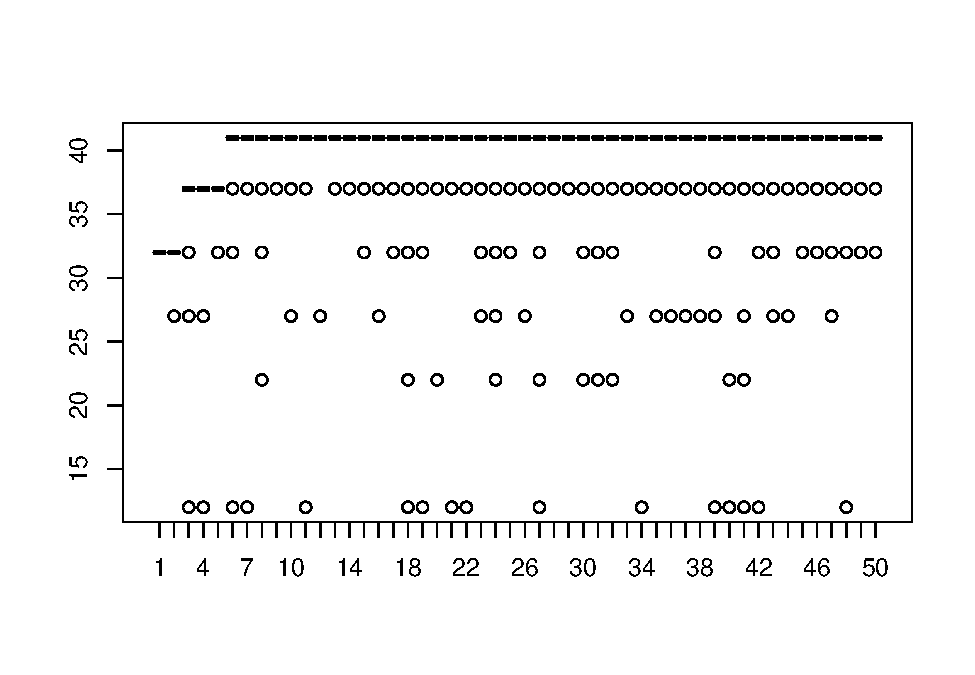
\includegraphics{_main_files/figure-latex/visualizeq-qs-count-1.pdf}

\hypertarget{salmon}{%
\section{Salmon}\label{salmon}}

Let's go through using salmon to count reads directly from the trimmed fastq.gz files

\hypertarget{pseudomapping-counting}{%
\subsection{Pseudomapping \& Counting}\label{pseudomapping-counting}}

\begin{Shaded}
\begin{Highlighting}[]
\VariableTok{DATA\_DIR}\OperatorTok{=}\StringTok{"/Users/}\VariableTok{$USER}\StringTok{/Desktop/Genomic\_Data\_Analysis/Data/Trimmed\_rfastp"}
\VariableTok{SALMON\_OUT\_DIR}\OperatorTok{=}\StringTok{"/Users/}\VariableTok{$USER}\StringTok{/Desktop/Genomic\_Data\_Analysis/Data/Counts/Salmon"}
\VariableTok{SALMON\_INDEX\_DIR}\OperatorTok{=}\StringTok{"/Users/}\VariableTok{$USER}\StringTok{/Desktop/Genomic\_Data\_Analysis/Reference/index\_salmon\_Saccharomyces\_cerevisiae.R64{-}1{-}1"}

\CommentTok{\# make the analysis directory if it doesn\textquotesingle{}t already exist}
\FunctionTok{mkdir} \AttributeTok{{-}p} \VariableTok{$SALMON\_OUT\_DIR}

\CommentTok{\# activate the salmon environment}
\ExtensionTok{conda}\NormalTok{ activate salmon}

\CommentTok{\# loop through all of the fastq files}
\ControlFlowTok{for}\NormalTok{ fn }\KeywordTok{in} \VariableTok{$DATA\_DIR}\NormalTok{/}\PreprocessorTok{*}\NormalTok{.fastq.gz}\KeywordTok{;}
\ControlFlowTok{do}
\VariableTok{samp}\OperatorTok{=}\KeywordTok{\textasciigrave{}}\FunctionTok{basename} \VariableTok{$\{fn\}}\KeywordTok{\textasciigrave{}}
\BuiltInTok{echo} \StringTok{"Processing sample }\VariableTok{$\{samp\}}\StringTok{"}

\CommentTok{\# run salmon}
\ExtensionTok{salmon}\NormalTok{ quant }\AttributeTok{{-}i} \VariableTok{$SALMON\_INDEX\_DIR} \AttributeTok{{-}l}\NormalTok{ A }\DataTypeTok{\textbackslash{}}
         \AttributeTok{{-}r} \VariableTok{$\{fn\}} \DataTypeTok{\textbackslash{}}
         \AttributeTok{{-}{-}useVBOpt} \DataTypeTok{\textbackslash{}}
         \AttributeTok{{-}p}\NormalTok{ 4 }\AttributeTok{{-}{-}validateMappings} \AttributeTok{{-}o} \VariableTok{$SALMON\_OUT\_DIR}\NormalTok{/}\VariableTok{$\{samp\}}\NormalTok{\_quant}
\ControlFlowTok{done}

\CommentTok{\# combine all of the output files into a merged count matrix}
\ExtensionTok{salmon}\NormalTok{ quantmerge }\AttributeTok{{-}{-}quants} \VariableTok{$SALMON\_OUT\_DIR}\NormalTok{/}\PreprocessorTok{*}\NormalTok{\_quant }\AttributeTok{{-}{-}column}\NormalTok{ numreads }\AttributeTok{{-}o} \VariableTok{$SALMON\_OUT\_DIR}\NormalTok{/salmon.gene\_counts.merged.yeast.tsv }

\CommentTok{\# remove the \_mRNA from gene name}
\FunctionTok{sed} \AttributeTok{{-}i} \StringTok{\textquotesingle{}\textquotesingle{}} \AttributeTok{{-}E} \StringTok{\textquotesingle{}s/\^{}([\^{}\textbackslash{}t]+)\_mRNA(\textbackslash{}t|$)/\textbackslash{}1\textbackslash{}2/\textquotesingle{}} \VariableTok{$SALMON\_OUT\_DIR}\NormalTok{/salmon.gene\_counts.merged.yeast.tsv}

\CommentTok{\# we can also create a table of tpm values per gene by changing the {-}{-}column flag}
\ExtensionTok{salmon}\NormalTok{ quantmerge }\AttributeTok{{-}{-}quants} \VariableTok{$SALMON\_OUT\_DIR}\NormalTok{/}\PreprocessorTok{*}\NormalTok{\_quant }\AttributeTok{{-}{-}column}\NormalTok{ tpm }\DataTypeTok{\textbackslash{}}
          \AttributeTok{{-}o} \VariableTok{$SALMON\_OUT\_DIR}\NormalTok{/salmon.gene\_tpm.merged.yeast.tsv}

\CommentTok{\# remove the \_mRNA from gene name}
\FunctionTok{sed} \AttributeTok{{-}i} \StringTok{\textquotesingle{}\textquotesingle{}} \AttributeTok{{-}E} \StringTok{\textquotesingle{}s/\^{}([\^{}\textbackslash{}t]+)\_mRNA(\textbackslash{}t|$)/\textbackslash{}1\textbackslash{}2/\textquotesingle{}} \VariableTok{$SALMON\_OUT\_DIR}\NormalTok{/salmon.gene\_tpm.merged.yeast.tsv}

\ExtensionTok{conda}\NormalTok{ deactivate}
\end{Highlighting}
\end{Shaded}

\begin{verbatim}
## Processing sample YPS606_MSN24_ETOH_REP1_R1.fastq.gz
## Version Info: This is the most recent version of salmon.
## ### salmon (selective-alignment-based) v1.10.0
## ### [ program ] => salmon 
## ### [ command ] => quant 
## ### [ index ] => { /Users/clstacy/Desktop/Genomic_Data_Analysis/Reference/index_salmon_Saccharomyces_cerevisiae.R64-1-1 }
## ### [ libType ] => { A }
## ### [ unmatedReads ] => { /Users/clstacy/Desktop/Genomic_Data_Analysis/Data/Trimmed_rfastp/YPS606_MSN24_ETOH_REP1_R1.fastq.gz }
## ### [ useVBOpt ] => { }
## ### [ threads ] => { 4 }
## ### [ validateMappings ] => { }
## ### [ output ] => { /Users/clstacy/Desktop/Genomic_Data_Analysis/Data/Counts/Salmon/YPS606_MSN24_ETOH_REP1_R1.fastq.gz_quant }
## Logs will be written to /Users/clstacy/Desktop/Genomic_Data_Analysis/Data/Counts/Salmon/YPS606_MSN24_ETOH_REP1_R1.fastq.gz_quant/logs
## [2023-10-26 16:17:04.631] [jointLog] [info] setting maxHashResizeThreads to 4
## -----------------------------------------
## | Loading contig table | Time = 5.8861 ms
## -----------------------------------------
## size = 25029
## -----------------------------------------
## | Loading contig offsets | Time = 1.2828 ms
## -----------------------------------------
## -----------------------------------------
## | Loading reference lengths | Time = 134.71 us
## -----------------------------------------
## -----------------------------------------
## | Loading mphf table | Time = 9.7713 ms
## -----------------------------------------
## size = 12321058
## [2023-10-26 16:17:04.632] [jointLog] [info] Fragment incompatibility prior below threshold.  Incompatible fragments will be ignored.
## [2023-10-26 16:17:04.632] [jointLog] [info] Usage of --validateMappings implies use of minScoreFraction. Since not explicitly specified, it is being set to 0.65
## [2023-10-26 16:17:04.632] [jointLog] [info] Setting consensusSlack to selective-alignment default of 0.35.
## [2023-10-26 16:17:04.632] [jointLog] [info] parsing read library format
## [2023-10-26 16:17:04.633] [jointLog] [info] There is 1 library.
## [2023-10-26 16:17:04.635] [jointLog] [info] Loading pufferfish index
## [2023-10-26 16:17:04.635] [jointLog] [info] Loading dense pufferfish index.
## Number of ones: 25028
## Number of ones per inventory item: 512
## Inventory entries filled: 49
## -----------------------------------------
## | Loading contig boundaries | Time = 27.891 ms
## -----------------------------------------
## size = 12321058
## -----------------------------------------
## | Loading sequence | Time = 3.9378 ms
## -----------------------------------------
## size = 11570218
## -----------------------------------------
## | Loading positions | Time = 53.427 ms
## -----------------------------------------
## size = 20892357
## -----------------------------------------
## | Loading reference sequence | Time = 6.1746 ms
## -----------------------------------------
## -----------------------------------------
## | Loading reference accumulative lengths | Time = 592.67 us
## -----------------------------------------
## [2023-10-26 16:17:04.746] [jointLog] [info] done
## [2023-10-26 16:17:04.832] [jointLog] [info] Index contained 6,588 targets
## [2023-10-26 16:17:04.833] [jointLog] [info] Number of decoys : 17
## [2023-10-26 16:17:04.833] [jointLog] [info] First decoy index : 6,571 
## 
## 
## 
## 
## [2023-10-26 16:17:05.026] [jointLog] [info] Automatically detected most likely library type as SR
## 
## 
## 
## 
## 
## 
## 
## 
## 
## [2023-10-26 16:17:05.467] [jointLog] [info] Thread saw mini-batch with a maximum of 1.32% zero probability fragments
## [2023-10-26 16:17:05.493] [jointLog] [info] Thread saw mini-batch with a maximum of 1.40% zero probability fragments
## [2023-10-26 16:17:05.495] [jointLog] [info] Thread saw mini-batch with a maximum of 1.22% zero probability fragments
## [2023-10-26 16:17:05.503] [jointLog] [info] Thread saw mini-batch with a maximum of 1.32% zero probability fragments
## [2023-10-26 16:17:05.524] [jointLog] [info] Computed 5,478 rich equivalence classes for further processing
## [2023-10-26 16:17:05.524] [jointLog] [info] Counted 186,106 total reads in the equivalence classes 
## [2023-10-26 16:17:05.530] [jointLog] [info] Number of mappings discarded because of alignment score : 31,126
## [2023-10-26 16:17:05.530] [jointLog] [info] Number of fragments entirely discarded because of alignment score : 7,997
## [2023-10-26 16:17:05.530] [jointLog] [info] Number of fragments discarded because they are best-mapped to decoys : 6,248
## [2023-10-26 16:17:05.530] [jointLog] [info] Number of fragments discarded because they have only dovetail (discordant) mappings to valid targets : 0
## [2023-10-26 16:17:05.530] [jointLog] [warning] Only 186106 fragments were mapped, but the number of burn-in fragments was set to 5000000.
## The effective lengths have been computed using the observed mappings.
## 
## [2023-10-26 16:17:05.530] [jointLog] [info] Mapping rate = 79.7786%
## 
## [2023-10-26 16:17:05.530] [jointLog] [info] finished quantifyLibrary()
## [2023-10-26 16:17:05.532] [jointLog] [info] Starting optimizer
## [2023-10-26 16:17:05.537] [jointLog] [info] Marked 0 weighted equivalence classes as degenerate
## [2023-10-26 16:17:05.548] [jointLog] [info] iteration = 0 | max rel diff. = 2057.36
## [2023-10-26 16:17:06.838] [jointLog] [info] iteration = 100 | max rel diff. = 0.000215288
## [2023-10-26 16:17:06.838] [jointLog] [info] Finished optimizer
## [2023-10-26 16:17:06.838] [jointLog] [info] writing output 
## 
## Processing sample YPS606_MSN24_ETOH_REP2_R1.fastq.gz
## Version Info: This is the most recent version of salmon.
## ### salmon (selective-alignment-based) v1.10.0
## ### [ program ] => salmon 
## ### [ command ] => quant 
## ### [ index ] => { /Users/clstacy/Desktop/Genomic_Data_Analysis/Reference/index_salmon_Saccharomyces_cerevisiae.R64-1-1 }
## ### [ libType ] => { A }
## ### [ unmatedReads ] => { /Users/clstacy/Desktop/Genomic_Data_Analysis/Data/Trimmed_rfastp/YPS606_MSN24_ETOH_REP2_R1.fastq.gz }
## ### [ useVBOpt ] => { }
## ### [ threads ] => { 4 }
## ### [ validateMappings ] => { }
## ### [ output ] => { /Users/clstacy/Desktop/Genomic_Data_Analysis/Data/Counts/Salmon/YPS606_MSN24_ETOH_REP2_R1.fastq.gz_quant }
## Logs will be written to /Users/clstacy/Desktop/Genomic_Data_Analysis/Data/Counts/Salmon/YPS606_MSN24_ETOH_REP2_R1.fastq.gz_quant/logs
## [2023-10-26 16:17:07.815] [jointLog] [info] setting maxHashResizeThreads to 4
## [2023-10-26 16:17:07.816] [jointLog] [info] Fragment incompatibility prior below threshold.  Incompatible fragments will be ignored.
## [2023-10-26 16:17:07.816] [jointLog] [info] Usage of --validateMappings implies use of minScoreFraction. Since not explicitly specified, it is being set to 0.65
## [2023-10-26 16:17:07.816] [jointLog] [info] Setting consensusSlack to selective-alignment default of 0.35.
## [2023-10-26 16:17:07.816] [jointLog] [info] parsing read library format
## [2023-10-26 16:17:07.816] [jointLog] [info] There is 1 library.
## -----------------------------------------
## | Loading contig table | Time = 3.4287 ms
## -----------------------------------------
## size = 25029
## -----------------------------------------
## | Loading contig offsets | Time = 107.12 us
## -----------------------------------------
## -----------------------------------------
## | Loading reference lengths | Time = 30.959 us
## -----------------------------------------
## -----------------------------------------
## | Loading mphf table | Time = 5.9727 ms
## -----------------------------------------
## size = 12321058
## Number of ones: 25028
## Number of ones per inventory item: 512
## Inventory entries filled: 49
## [2023-10-26 16:17:07.816] [jointLog] [info] Loading pufferfish index
## [2023-10-26 16:17:07.816] [jointLog] [info] Loading dense pufferfish index.
## -----------------------------------------
## | Loading contig boundaries | Time = 26.454 ms
## -----------------------------------------
## size = 12321058
## -----------------------------------------
## | Loading sequence | Time = 2.4621 ms
## -----------------------------------------
## size = 11570218
## -----------------------------------------
## | Loading positions | Time = 27.425 ms
## -----------------------------------------
## size = 20892357
## -----------------------------------------
## | Loading reference sequence | Time = 4.0427 ms
## -----------------------------------------
## -----------------------------------------
## | Loading reference accumulative lengths | Time = 95.542 us
## -----------------------------------------
## [2023-10-26 16:17:07.886] [jointLog] [info] done
## [2023-10-26 16:17:07.955] [jointLog] [info] Index contained 6,588 targets
## [2023-10-26 16:17:07.956] [jointLog] [info] Number of decoys : 17
## [2023-10-26 16:17:07.956] [jointLog] [info] First decoy index : 6,571 
## 
## 
## 
## 
## [2023-10-26 16:17:08.123] [jointLog] [info] Automatically detected most likely library type as SR
## 
## 
## 
## 
## 
## 
## 
## 
## 
## [2023-10-26 16:17:08.390] [jointLog] [info] Thread saw mini-batch with a maximum of 1.32% zero probability fragments
## [2023-10-26 16:17:08.391] [jointLog] [info] Thread saw mini-batch with a maximum of 1.40% zero probability fragments
## [2023-10-26 16:17:08.402] [jointLog] [info] Thread saw mini-batch with a maximum of 1.18% zero probability fragments
## [2023-10-26 16:17:08.408] [jointLog] [info] Thread saw mini-batch with a maximum of 1.24% zero probability fragments
## [2023-10-26 16:17:08.425] [jointLog] [info] Computed 5,294 rich equivalence classes for further processing
## [2023-10-26 16:17:08.425] [jointLog] [info] Counted 173,318 total reads in the equivalence classes 
## [2023-10-26 16:17:08.430] [jointLog] [info] Number of mappings discarded because of alignment score : 25,173
## [2023-10-26 16:17:08.430] [jointLog] [info] Number of fragments entirely discarded because of alignment score : 7,099
## [2023-10-26 16:17:08.430] [jointLog] [info] Number of fragments discarded because they are best-mapped to decoys : 5,772
## [2023-10-26 16:17:08.430] [jointLog] [info] Number of fragments discarded because they have only dovetail (discordant) mappings to valid targets : 0
## [2023-10-26 16:17:08.430] [jointLog] [warning] Only 173318 fragments were mapped, but the number of burn-in fragments was set to 5000000.
## The effective lengths have been computed using the observed mappings.
## 
## [2023-10-26 16:17:08.430] [jointLog] [info] Mapping rate = 80.3105%
## 
## [2023-10-26 16:17:08.430] [jointLog] [info] finished quantifyLibrary()
## [2023-10-26 16:17:08.431] [jointLog] [info] Starting optimizer
## [2023-10-26 16:17:08.433] [jointLog] [info] Marked 0 weighted equivalence classes as degenerate
## [2023-10-26 16:17:08.442] [jointLog] [info] iteration = 0 | max rel diff. = 1476.42
## [2023-10-26 16:17:09.772] [jointLog] [info] iteration = 100 | max rel diff. = 0.000932656
## [2023-10-26 16:17:09.772] [jointLog] [info] Finished optimizer
## [2023-10-26 16:17:09.772] [jointLog] [info] writing output 
## 
## Processing sample YPS606_MSN24_ETOH_REP3_R1.fastq.gz
## Version Info: This is the most recent version of salmon.
## ### salmon (selective-alignment-based) v1.10.0
## ### [ program ] => salmon 
## ### [ command ] => quant 
## ### [ index ] => { /Users/clstacy/Desktop/Genomic_Data_Analysis/Reference/index_salmon_Saccharomyces_cerevisiae.R64-1-1 }
## ### [ libType ] => { A }
## ### [ unmatedReads ] => { /Users/clstacy/Desktop/Genomic_Data_Analysis/Data/Trimmed_rfastp/YPS606_MSN24_ETOH_REP3_R1.fastq.gz }
## ### [ useVBOpt ] => { }
## ### [ threads ] => { 4 }
## ### [ validateMappings ] => { }
## ### [ output ] => { /Users/clstacy/Desktop/Genomic_Data_Analysis/Data/Counts/Salmon/YPS606_MSN24_ETOH_REP3_R1.fastq.gz_quant }
## Logs will be written to /Users/clstacy/Desktop/Genomic_Data_Analysis/Data/Counts/Salmon/YPS606_MSN24_ETOH_REP3_R1.fastq.gz_quant/logs
## [2023-10-26 16:17:10.437] [jointLog] [info] setting maxHashResizeThreads to 4
## [2023-10-26 16:17:10.438] [jointLog] [info] Fragment incompatibility prior below threshold.  Incompatible fragments will be ignored.
## [2023-10-26 16:17:10.438] [jointLog] [info] Usage of --validateMappings implies use of minScoreFraction. Since not explicitly specified, it is being set to 0.65
## [2023-10-26 16:17:10.438] [jointLog] [info] Setting consensusSlack to selective-alignment default of 0.35.
## [2023-10-26 16:17:10.438] [jointLog] [info] parsing read library format
## [2023-10-26 16:17:10.438] [jointLog] [info] There is 1 library.
## -----------------------------------------
## | Loading contig table | Time = 4.2352 ms
## -----------------------------------------
## size = 25029
## -----------------------------------------
## | Loading contig offsets | Time = 105.79 us
## -----------------------------------------
## -----------------------------------------
## | Loading reference lengths | Time = 30.458 us
## -----------------------------------------
## -----------------------------------------
## | Loading mphf table | Time = 6.0489 ms
## -----------------------------------------
## size = 12321058
## Number of ones: 25028
## Number of ones per inventory item: 512
## Inventory entries filled: 49
## [2023-10-26 16:17:10.438] [jointLog] [info] Loading pufferfish index
## [2023-10-26 16:17:10.438] [jointLog] [info] Loading dense pufferfish index.
## -----------------------------------------
## | Loading contig boundaries | Time = 26.492 ms
## -----------------------------------------
## size = 12321058
## -----------------------------------------
## | Loading sequence | Time = 2.4975 ms
## -----------------------------------------
## size = 11570218
## -----------------------------------------
## | Loading positions | Time = 26.471 ms
## -----------------------------------------
## size = 20892357
## -----------------------------------------
## | Loading reference sequence | Time = 4.0636 ms
## -----------------------------------------
## -----------------------------------------
## | Loading reference accumulative lengths | Time = 66.334 us
## -----------------------------------------
## [2023-10-26 16:17:10.508] [jointLog] [info] done
## [2023-10-26 16:17:10.583] [jointLog] [info] Index contained 6,588 targets
## [2023-10-26 16:17:10.584] [jointLog] [info] Number of decoys : 17
## [2023-10-26 16:17:10.584] [jointLog] [info] First decoy index : 6,571 
## 
## 
## 
## 
## [2023-10-26 16:17:10.770] [jointLog] [info] Automatically detected most likely library type as SR
## 
## 
## 
## 
## 
## 
## 
## 
## 
## [2023-10-26 16:17:11.107] [jointLog] [info] Thread saw mini-batch with a maximum of 1.58% zero probability fragments
## [2023-10-26 16:17:11.128] [jointLog] [info] Thread saw mini-batch with a maximum of 1.56% zero probability fragments
## [2023-10-26 16:17:11.130] [jointLog] [info] Thread saw mini-batch with a maximum of 1.52% zero probability fragments
## [2023-10-26 16:17:11.131] [jointLog] [info] Thread saw mini-batch with a maximum of 1.55% zero probability fragments
## [2023-10-26 16:17:11.172] [jointLog] [info] Computed 5,306 rich equivalence classes for further processing
## [2023-10-26 16:17:11.172] [jointLog] [info] Counted 158,068 total reads in the equivalence classes 
## [2023-10-26 16:17:11.178] [jointLog] [info] Number of mappings discarded because of alignment score : 19,662
## [2023-10-26 16:17:11.178] [jointLog] [info] Number of fragments entirely discarded because of alignment score : 6,467
## [2023-10-26 16:17:11.178] [jointLog] [info] Number of fragments discarded because they are best-mapped to decoys : 4,929
## [2023-10-26 16:17:11.178] [jointLog] [info] Number of fragments discarded because they have only dovetail (discordant) mappings to valid targets : 0
## [2023-10-26 16:17:11.179] [jointLog] [warning] Only 158068 fragments were mapped, but the number of burn-in fragments was set to 5000000.
## The effective lengths have been computed using the observed mappings.
## 
## [2023-10-26 16:17:11.179] [jointLog] [info] Mapping rate = 79.4008%
## 
## [2023-10-26 16:17:11.179] [jointLog] [info] finished quantifyLibrary()
## [2023-10-26 16:17:11.179] [jointLog] [info] Starting optimizer
## [2023-10-26 16:17:11.183] [jointLog] [info] Marked 0 weighted equivalence classes as degenerate
## [2023-10-26 16:17:11.198] [jointLog] [info] iteration = 0 | max rel diff. = 483.863
## [2023-10-26 16:17:12.422] [jointLog] [info] iteration = 100 | max rel diff. = 0.000307319
## [2023-10-26 16:17:12.423] [jointLog] [info] Finished optimizer
## [2023-10-26 16:17:12.423] [jointLog] [info] writing output 
## 
## Processing sample YPS606_MSN24_ETOH_REP4_R1.fastq.gz
## Version Info: This is the most recent version of salmon.
## ### salmon (selective-alignment-based) v1.10.0
## ### [ program ] => salmon 
## ### [ command ] => quant 
## ### [ index ] => { /Users/clstacy/Desktop/Genomic_Data_Analysis/Reference/index_salmon_Saccharomyces_cerevisiae.R64-1-1 }
## ### [ libType ] => { A }
## ### [ unmatedReads ] => { /Users/clstacy/Desktop/Genomic_Data_Analysis/Data/Trimmed_rfastp/YPS606_MSN24_ETOH_REP4_R1.fastq.gz }
## ### [ useVBOpt ] => { }
## ### [ threads ] => { 4 }
## ### [ validateMappings ] => { }
## ### [ output ] => { /Users/clstacy/Desktop/Genomic_Data_Analysis/Data/Counts/Salmon/YPS606_MSN24_ETOH_REP4_R1.fastq.gz_quant }
## Logs will be written to /Users/clstacy/Desktop/Genomic_Data_Analysis/Data/Counts/Salmon/YPS606_MSN24_ETOH_REP4_R1.fastq.gz_quant/logs
## [2023-10-26 16:17:13.364] [jointLog] [info] setting maxHashResizeThreads to 4
## [2023-10-26 16:17:13.364] [jointLog] [info] Fragment incompatibility prior below threshold.  Incompatible fragments will be ignored.
## [2023-10-26 16:17:13.364] [jointLog] [info] Usage of --validateMappings implies use of minScoreFraction. Since not explicitly specified, it is being set to 0.65
## [2023-10-26 16:17:13.364] [jointLog] [info] Setting consensusSlack to selective-alignment default of 0.35.
## [2023-10-26 16:17:13.364] [jointLog] [info] parsing read library format
## [2023-10-26 16:17:13.364] [jointLog] [info] There is 1 library.
## -----------------------------------------
## | Loading contig table | Time = 5.372 ms
## -----------------------------------------
## size = 25029
## -----------------------------------------
## | Loading contig offsets | Time = 341.25 us
## -----------------------------------------
## -----------------------------------------
## | Loading reference lengths | Time = 94.625 us
## -----------------------------------------
## -----------------------------------------
## | Loading mphf table | Time = 13.219 ms
## -----------------------------------------
## size = 12321058
## Number of ones: 25028
## Number of ones per inventory item: 512
## [2023-10-26 16:17:13.365] [jointLog] [info] Loading pufferfish index
## [2023-10-26 16:17:13.365] [jointLog] [info] Loading dense pufferfish index.
## Inventory entries filled: 49
## -----------------------------------------
## | Loading contig boundaries | Time = 34.804 ms
## -----------------------------------------
## size = 12321058
## -----------------------------------------
## | Loading sequence | Time = 2.5577 ms
## -----------------------------------------
## size = 11570218
## -----------------------------------------
## | Loading positions | Time = 30.303 ms
## -----------------------------------------
## size = 20892357
## -----------------------------------------
## | Loading reference sequence | Time = 4.9481 ms
## -----------------------------------------
## -----------------------------------------
## | Loading reference accumulative lengths | Time = 78.25 us
## -----------------------------------------
## [2023-10-26 16:17:13.457] [jointLog] [info] done
## [2023-10-26 16:17:13.559] [jointLog] [info] Index contained 6,588 targets
## [2023-10-26 16:17:13.560] [jointLog] [info] Number of decoys : 17
## [2023-10-26 16:17:13.560] [jointLog] [info] First decoy index : 6,571 
## 
## 
## 
## 
## [2023-10-26 16:17:13.825] [jointLog] [info] Automatically detected most likely library type as SR
## 
## [2023-10-26 16:17:14.348] [jointLog] [info] Thread saw mini-batch with a maximum of 1.18% zero probability fragments
## [2023-10-26 16:17:14.349] [jointLog] [info] Thread saw mini-batch with a maximum of 1.32% zero probability fragments
## [2023-10-26 16:17:14.352] [jointLog] [info] Thread saw mini-batch with a maximum of 1.26% zero probability fragments
## [2023-10-26 16:17:14.369] [jointLog] [info] Thread saw mini-batch with a maximum of 1.30% zero probability fragments
## 
## 
## 
## 
## [2023-10-26 16:17:14.399] [jointLog] [info] Computed 5,260 rich equivalence classes for further processing
## [2023-10-26 16:17:14.399] [jointLog] [info] Counted 165,612 total reads in the equivalence classes 
## 
## 
## 
## 
## [2023-10-26 16:17:14.404] [jointLog] [info] Number of mappings discarded because of alignment score : 20,744
## [2023-10-26 16:17:14.404] [jointLog] [info] Number of fragments entirely discarded because of alignment score : 6,497
## [2023-10-26 16:17:14.404] [jointLog] [info] Number of fragments discarded because they are best-mapped to decoys : 5,015
## [2023-10-26 16:17:14.404] [jointLog] [info] Number of fragments discarded because they have only dovetail (discordant) mappings to valid targets : 0
## [2023-10-26 16:17:14.404] [jointLog] [warning] Only 165612 fragments were mapped, but the number of burn-in fragments was set to 5000000.
## The effective lengths have been computed using the observed mappings.
## 
## [2023-10-26 16:17:14.404] [jointLog] [info] Mapping rate = 80.4754%
## 
## [2023-10-26 16:17:14.404] [jointLog] [info] finished quantifyLibrary()
## [2023-10-26 16:17:14.405] [jointLog] [info] Starting optimizer
## [2023-10-26 16:17:14.408] [jointLog] [info] Marked 0 weighted equivalence classes as degenerate
## [2023-10-26 16:17:14.416] [jointLog] [info] iteration = 0 | max rel diff. = 1859.16
## [2023-10-26 16:17:15.677] [jointLog] [info] iteration = 100 | max rel diff. = 0.000249187
## [2023-10-26 16:17:15.677] [jointLog] [info] Finished optimizer
## [2023-10-26 16:17:15.677] [jointLog] [info] writing output 
## 
## Processing sample YPS606_MSN24_MOCK_REP1_R1.fastq.gz
## Version Info: This is the most recent version of salmon.
## ### salmon (selective-alignment-based) v1.10.0
## ### [ program ] => salmon 
## ### [ command ] => quant 
## ### [ index ] => { /Users/clstacy/Desktop/Genomic_Data_Analysis/Reference/index_salmon_Saccharomyces_cerevisiae.R64-1-1 }
## ### [ libType ] => { A }
## ### [ unmatedReads ] => { /Users/clstacy/Desktop/Genomic_Data_Analysis/Data/Trimmed_rfastp/YPS606_MSN24_MOCK_REP1_R1.fastq.gz }
## ### [ useVBOpt ] => { }
## ### [ threads ] => { 4 }
## ### [ validateMappings ] => { }
## ### [ output ] => { /Users/clstacy/Desktop/Genomic_Data_Analysis/Data/Counts/Salmon/YPS606_MSN24_MOCK_REP1_R1.fastq.gz_quant }
## Logs will be written to /Users/clstacy/Desktop/Genomic_Data_Analysis/Data/Counts/Salmon/YPS606_MSN24_MOCK_REP1_R1.fastq.gz_quant/logs
## [2023-10-26 16:17:16.442] [jointLog] [info] setting maxHashResizeThreads to 4
## [2023-10-26 16:17:16.442] [jointLog] [info] Fragment incompatibility prior below threshold.  Incompatible fragments will be ignored.
## [2023-10-26 16:17:16.442] [jointLog] [info] Usage of --validateMappings implies use of minScoreFraction. Since not explicitly specified, it is being set to 0.65
## [2023-10-26 16:17:16.442] [jointLog] [info] Setting consensusSlack to selective-alignment default of 0.35.
## [2023-10-26 16:17:16.442] [jointLog] [info] parsing read library format
## [2023-10-26 16:17:16.442] [jointLog] [info] There is 1 library.
## -----------------------------------------
## | Loading contig table | Time = 3.5938 ms
## -----------------------------------------
## size = 25029
## -----------------------------------------
## | Loading contig offsets | Time = 113.75 us
## -----------------------------------------
## -----------------------------------------
## | Loading reference lengths | Time = 29.417 us
## -----------------------------------------
## -----------------------------------------
## | Loading mphf table | Time = 5.8898 ms
## -----------------------------------------
## size = 12321058
## Number of ones: 25028
## Number of ones per inventory item: 512
## Inventory entries filled: 49
## [2023-10-26 16:17:16.442] [jointLog] [info] Loading pufferfish index
## [2023-10-26 16:17:16.442] [jointLog] [info] Loading dense pufferfish index.
## -----------------------------------------
## | Loading contig boundaries | Time = 26.204 ms
## -----------------------------------------
## size = 12321058
## -----------------------------------------
## | Loading sequence | Time = 2.4212 ms
## -----------------------------------------
## size = 11570218
## -----------------------------------------
## | Loading positions | Time = 26.389 ms
## -----------------------------------------
## size = 20892357
## -----------------------------------------
## | Loading reference sequence | Time = 4.0679 ms
## -----------------------------------------
## -----------------------------------------
## | Loading reference accumulative lengths | Time = 61.167 us
## -----------------------------------------
## [2023-10-26 16:17:16.512] [jointLog] [info] done
## [2023-10-26 16:17:16.588] [jointLog] [info] Index contained 6,588 targets
## [2023-10-26 16:17:16.589] [jointLog] [info] Number of decoys : 17
## [2023-10-26 16:17:16.589] [jointLog] [info] First decoy index : 6,571 
## 
## 
## 
## 
## [2023-10-26 16:17:16.757] [jointLog] [info] Automatically detected most likely library type as SR
## 
## [2023-10-26 16:17:16.937] [jointLog] [info] Thread saw mini-batch with a maximum of 1.16% zero probability fragments
## [2023-10-26 16:17:16.939] [jointLog] [info] Thread saw mini-batch with a maximum of 1.20% zero probability fragments
## [2023-10-26 16:17:16.941] [jointLog] [info] Thread saw mini-batch with a maximum of 1.20% zero probability fragments
## 
## 
## 
## 
## [2023-10-26 16:17:16.957] [jointLog] [info] Thread saw mini-batch with a maximum of 1.20% zero probability fragments
## [2023-10-26 16:17:16.974] [jointLog] [info] Computed 5,122 rich equivalence classes for further processing
## [2023-10-26 16:17:16.974] [jointLog] [info] Counted 130,772 total reads in the equivalence classes 
## 
## 
## 
## 
## [2023-10-26 16:17:16.979] [jointLog] [info] Number of mappings discarded because of alignment score : 28,846
## [2023-10-26 16:17:16.979] [jointLog] [info] Number of fragments entirely discarded because of alignment score : 6,943
## [2023-10-26 16:17:16.979] [jointLog] [info] Number of fragments discarded because they are best-mapped to decoys : 5,380
## [2023-10-26 16:17:16.979] [jointLog] [info] Number of fragments discarded because they have only dovetail (discordant) mappings to valid targets : 0
## [2023-10-26 16:17:16.980] [jointLog] [warning] Only 130772 fragments were mapped, but the number of burn-in fragments was set to 5000000.
## The effective lengths have been computed using the observed mappings.
## 
## [2023-10-26 16:17:16.980] [jointLog] [info] Mapping rate = 78.2714%
## 
## [2023-10-26 16:17:16.980] [jointLog] [info] finished quantifyLibrary()
## [2023-10-26 16:17:16.980] [jointLog] [info] Starting optimizer
## [2023-10-26 16:17:16.983] [jointLog] [info] Marked 0 weighted equivalence classes as degenerate
## [2023-10-26 16:17:16.994] [jointLog] [info] iteration = 0 | max rel diff. = 1687.17
## [2023-10-26 16:17:18.281] [jointLog] [info] iteration = 100 | max rel diff. = 0.000122454
## [2023-10-26 16:17:18.281] [jointLog] [info] Finished optimizer
## [2023-10-26 16:17:18.281] [jointLog] [info] writing output 
## 
## Processing sample YPS606_MSN24_MOCK_REP2_R1.fastq.gz
## Version Info: This is the most recent version of salmon.
## ### salmon (selective-alignment-based) v1.10.0
## ### [ program ] => salmon 
## ### [ command ] => quant 
## ### [ index ] => { /Users/clstacy/Desktop/Genomic_Data_Analysis/Reference/index_salmon_Saccharomyces_cerevisiae.R64-1-1 }
## ### [ libType ] => { A }
## ### [ unmatedReads ] => { /Users/clstacy/Desktop/Genomic_Data_Analysis/Data/Trimmed_rfastp/YPS606_MSN24_MOCK_REP2_R1.fastq.gz }
## ### [ useVBOpt ] => { }
## ### [ threads ] => { 4 }
## ### [ validateMappings ] => { }
## ### [ output ] => { /Users/clstacy/Desktop/Genomic_Data_Analysis/Data/Counts/Salmon/YPS606_MSN24_MOCK_REP2_R1.fastq.gz_quant }
## Logs will be written to /Users/clstacy/Desktop/Genomic_Data_Analysis/Data/Counts/Salmon/YPS606_MSN24_MOCK_REP2_R1.fastq.gz_quant/logs
## [2023-10-26 16:17:19.020] [jointLog] [info] setting maxHashResizeThreads to 4
## [2023-10-26 16:17:19.020] [jointLog] [info] Fragment incompatibility prior below threshold.  Incompatible fragments will be ignored.
## [2023-10-26 16:17:19.020] [jointLog] [info] Usage of --validateMappings implies use of minScoreFraction. Since not explicitly specified, it is being set to 0.65
## [2023-10-26 16:17:19.020] [jointLog] [info] Setting consensusSlack to selective-alignment default of 0.35.
## [2023-10-26 16:17:19.020] [jointLog] [info] parsing read library format
## [2023-10-26 16:17:19.020] [jointLog] [info] There is 1 library.
## -----------------------------------------
## | Loading contig table | Time = 5.0504 ms
## -----------------------------------------
## size = 25029
## -----------------------------------------
## | Loading contig offsets | Time = 155.67 us
## -----------------------------------------
## -----------------------------------------
## | Loading reference lengths | Time = 38.25 us
## -----------------------------------------
## -----------------------------------------
## | Loading mphf table | Time = 6.379 ms
## -----------------------------------------
## size = 12321058
## Number of ones: 25028
## Number of ones per inventory item: 512
## [2023-10-26 16:17:19.020] [jointLog] [info] Loading pufferfish index
## [2023-10-26 16:17:19.020] [jointLog] [info] Loading dense pufferfish index.
## Inventory entries filled: 49
## -----------------------------------------
## | Loading contig boundaries | Time = 27.051 ms
## -----------------------------------------
## size = 12321058
## -----------------------------------------
## | Loading sequence | Time = 2.3987 ms
## -----------------------------------------
## size = 11570218
## -----------------------------------------
## | Loading positions | Time = 26.53 ms
## -----------------------------------------
## size = 20892357
## -----------------------------------------
## | Loading reference sequence | Time = 4.0417 ms
## -----------------------------------------
## -----------------------------------------
## | Loading reference accumulative lengths | Time = 67.459 us
## -----------------------------------------
## [2023-10-26 16:17:19.093] [jointLog] [info] done
## [2023-10-26 16:17:19.159] [jointLog] [info] Index contained 6,588 targets
## [2023-10-26 16:17:19.160] [jointLog] [info] Number of decoys : 17
## [2023-10-26 16:17:19.160] [jointLog] [info] First decoy index : 6,571 
## 
## 
## 
## 
## [2023-10-26 16:17:19.333] [jointLog] [info] Automatically detected most likely library type as SR
## 
## [2023-10-26 16:17:19.522] [jointLog] [info] Thread saw mini-batch with a maximum of 1.10% zero probability fragments
## [2023-10-26 16:17:19.523] [jointLog] [info] Thread saw mini-batch with a maximum of 1.12% zero probability fragments
## [2023-10-26 16:17:19.543] [jointLog] [info] Thread saw mini-batch with a maximum of 1.14% zero probability fragments
## [2023-10-26 16:17:19.543] [jointLog] [info] Thread saw mini-batch with a maximum of 1.08% zero probability fragments
## 
## 
## 
## 
## 
## 
## 
## 
## [2023-10-26 16:17:19.562] [jointLog] [info] Computed 5,108 rich equivalence classes for further processing
## [2023-10-26 16:17:19.562] [jointLog] [info] Counted 135,236 total reads in the equivalence classes 
## [2023-10-26 16:17:19.569] [jointLog] [info] Number of mappings discarded because of alignment score : 19,440
## [2023-10-26 16:17:19.569] [jointLog] [info] Number of fragments entirely discarded because of alignment score : 5,837
## [2023-10-26 16:17:19.569] [jointLog] [info] Number of fragments discarded because they are best-mapped to decoys : 4,792
## [2023-10-26 16:17:19.569] [jointLog] [info] Number of fragments discarded because they have only dovetail (discordant) mappings to valid targets : 0
## [2023-10-26 16:17:19.569] [jointLog] [warning] Only 135236 fragments were mapped, but the number of burn-in fragments was set to 5000000.
## The effective lengths have been computed using the observed mappings.
## 
## [2023-10-26 16:17:19.569] [jointLog] [info] Mapping rate = 79.6659%
## 
## [2023-10-26 16:17:19.569] [jointLog] [info] finished quantifyLibrary()
## [2023-10-26 16:17:19.569] [jointLog] [info] Starting optimizer
## [2023-10-26 16:17:19.572] [jointLog] [info] Marked 0 weighted equivalence classes as degenerate
## [2023-10-26 16:17:19.586] [jointLog] [info] iteration = 0 | max rel diff. = 1365.21
## [2023-10-26 16:17:20.917] [jointLog] [info] iteration = 100 | max rel diff. = 0.00138657
## [2023-10-26 16:17:20.917] [jointLog] [info] Finished optimizer
## [2023-10-26 16:17:20.917] [jointLog] [info] writing output 
## 
## Processing sample YPS606_MSN24_MOCK_REP3_R1.fastq.gz
## Version Info: This is the most recent version of salmon.
## ### salmon (selective-alignment-based) v1.10.0
## ### [ program ] => salmon 
## ### [ command ] => quant 
## ### [ index ] => { /Users/clstacy/Desktop/Genomic_Data_Analysis/Reference/index_salmon_Saccharomyces_cerevisiae.R64-1-1 }
## ### [ libType ] => { A }
## ### [ unmatedReads ] => { /Users/clstacy/Desktop/Genomic_Data_Analysis/Data/Trimmed_rfastp/YPS606_MSN24_MOCK_REP3_R1.fastq.gz }
## ### [ useVBOpt ] => { }
## ### [ threads ] => { 4 }
## ### [ validateMappings ] => { }
## ### [ output ] => { /Users/clstacy/Desktop/Genomic_Data_Analysis/Data/Counts/Salmon/YPS606_MSN24_MOCK_REP3_R1.fastq.gz_quant }
## Logs will be written to /Users/clstacy/Desktop/Genomic_Data_Analysis/Data/Counts/Salmon/YPS606_MSN24_MOCK_REP3_R1.fastq.gz_quant/logs
## [2023-10-26 16:17:21.594] [jointLog] [info] setting maxHashResizeThreads to 4
## [2023-10-26 16:17:21.594] [jointLog] [info] Fragment incompatibility prior below threshold.  Incompatible fragments will be ignored.
## [2023-10-26 16:17:21.594] [jointLog] [info] Usage of --validateMappings implies use of minScoreFraction. Since not explicitly specified, it is being set to 0.65
## [2023-10-26 16:17:21.594] [jointLog] [info] Setting consensusSlack to selective-alignment default of 0.35.
## [2023-10-26 16:17:21.594] [jointLog] [info] parsing read library format
## [2023-10-26 16:17:21.594] [jointLog] [info] There is 1 library.
## -----------------------------------------
## | Loading contig table | Time = 4.415 ms
## -----------------------------------------
## size = 25029
## -----------------------------------------
## | Loading contig offsets | Time = 112.46 us
## -----------------------------------------
## -----------------------------------------
## | Loading reference lengths | Time = 29.542 us
## -----------------------------------------
## -----------------------------------------
## | Loading mphf table | Time = 5.8686 ms
## -----------------------------------------
## size = 12321058
## Number of ones: 25028
## Number of ones per inventory item: 512
## Inventory entries filled: 49
## [2023-10-26 16:17:21.594] [jointLog] [info] Loading pufferfish index
## [2023-10-26 16:17:21.594] [jointLog] [info] Loading dense pufferfish index.
## -----------------------------------------
## | Loading contig boundaries | Time = 26.337 ms
## -----------------------------------------
## size = 12321058
## -----------------------------------------
## | Loading sequence | Time = 2.5303 ms
## -----------------------------------------
## size = 11570218
## -----------------------------------------
## | Loading positions | Time = 26.461 ms
## -----------------------------------------
## size = 20892357
## -----------------------------------------
## | Loading reference sequence | Time = 4.1354 ms
## -----------------------------------------
## -----------------------------------------
## | Loading reference accumulative lengths | Time = 65.292 us
## -----------------------------------------
## [2023-10-26 16:17:21.664] [jointLog] [info] done
## [2023-10-26 16:17:21.732] [jointLog] [info] Index contained 6,588 targets
## [2023-10-26 16:17:21.733] [jointLog] [info] Number of decoys : 17
## [2023-10-26 16:17:21.733] [jointLog] [info] First decoy index : 6,571 
## 
## 
## 
## 
## [2023-10-26 16:17:21.910] [jointLog] [info] Automatically detected most likely library type as SR
## 
## 
## 
## 
## 
## 
## 
## 
## 
## [2023-10-26 16:17:22.203] [jointLog] [info] Thread saw mini-batch with a maximum of 1.62% zero probability fragments
## [2023-10-26 16:17:22.204] [jointLog] [info] Thread saw mini-batch with a maximum of 1.66% zero probability fragments
## [2023-10-26 16:17:22.228] [jointLog] [info] Thread saw mini-batch with a maximum of 1.58% zero probability fragments
## [2023-10-26 16:17:22.237] [jointLog] [info] Thread saw mini-batch with a maximum of 1.52% zero probability fragments
## [2023-10-26 16:17:22.260] [jointLog] [info] Computed 5,213 rich equivalence classes for further processing
## [2023-10-26 16:17:22.260] [jointLog] [info] Counted 161,108 total reads in the equivalence classes 
## [2023-10-26 16:17:22.266] [jointLog] [info] Number of mappings discarded because of alignment score : 23,201
## [2023-10-26 16:17:22.266] [jointLog] [info] Number of fragments entirely discarded because of alignment score : 7,784
## [2023-10-26 16:17:22.266] [jointLog] [info] Number of fragments discarded because they are best-mapped to decoys : 6,012
## [2023-10-26 16:17:22.266] [jointLog] [info] Number of fragments discarded because they have only dovetail (discordant) mappings to valid targets : 0
## [2023-10-26 16:17:22.267] [jointLog] [warning] Only 161108 fragments were mapped, but the number of burn-in fragments was set to 5000000.
## The effective lengths have been computed using the observed mappings.
## 
## [2023-10-26 16:17:22.267] [jointLog] [info] Mapping rate = 76.7177%
## 
## [2023-10-26 16:17:22.267] [jointLog] [info] finished quantifyLibrary()
## [2023-10-26 16:17:22.267] [jointLog] [info] Starting optimizer
## [2023-10-26 16:17:22.270] [jointLog] [info] Marked 0 weighted equivalence classes as degenerate
## [2023-10-26 16:17:22.283] [jointLog] [info] iteration = 0 | max rel diff. = 1651.76
## [2023-10-26 16:17:23.603] [jointLog] [info] iteration = 100 | max rel diff. = 0.00012575
## [2023-10-26 16:17:23.603] [jointLog] [info] Finished optimizer
## [2023-10-26 16:17:23.603] [jointLog] [info] writing output 
## 
## Processing sample YPS606_MSN24_MOCK_REP4_R1.fastq.gz
## Version Info: This is the most recent version of salmon.
## ### salmon (selective-alignment-based) v1.10.0
## ### [ program ] => salmon 
## ### [ command ] => quant 
## ### [ index ] => { /Users/clstacy/Desktop/Genomic_Data_Analysis/Reference/index_salmon_Saccharomyces_cerevisiae.R64-1-1 }
## ### [ libType ] => { A }
## ### [ unmatedReads ] => { /Users/clstacy/Desktop/Genomic_Data_Analysis/Data/Trimmed_rfastp/YPS606_MSN24_MOCK_REP4_R1.fastq.gz }
## ### [ useVBOpt ] => { }
## ### [ threads ] => { 4 }
## ### [ validateMappings ] => { }
## ### [ output ] => { /Users/clstacy/Desktop/Genomic_Data_Analysis/Data/Counts/Salmon/YPS606_MSN24_MOCK_REP4_R1.fastq.gz_quant }
## Logs will be written to /Users/clstacy/Desktop/Genomic_Data_Analysis/Data/Counts/Salmon/YPS606_MSN24_MOCK_REP4_R1.fastq.gz_quant/logs
## [2023-10-26 16:17:24.172] [jointLog] [info] setting maxHashResizeThreads to 4
## [2023-10-26 16:17:24.172] [jointLog] [info] Fragment incompatibility prior below threshold.  Incompatible fragments will be ignored.
## [2023-10-26 16:17:24.172] [jointLog] [info] Usage of --validateMappings implies use of minScoreFraction. Since not explicitly specified, it is being set to 0.65
## [2023-10-26 16:17:24.172] [jointLog] [info] Setting consensusSlack to selective-alignment default of 0.35.
## [2023-10-26 16:17:24.172] [jointLog] [info] parsing read library format
## [2023-10-26 16:17:24.172] [jointLog] [info] There is 1 library.
## -----------------------------------------
## | Loading contig table | Time = 3.5423 ms
## -----------------------------------------
## size = 25029
## -----------------------------------------
## | Loading contig offsets | Time = 131.25 us
## -----------------------------------------
## -----------------------------------------
## | Loading reference lengths | Time = 38.708 us
## -----------------------------------------
## -----------------------------------------
## | Loading mphf table | Time = 7.7895 ms
## -----------------------------------------
## size = 12321058
## Number of ones: 25028
## Number of ones per inventory item: 512
## [2023-10-26 16:17:24.172] [jointLog] [info] Loading pufferfish index
## [2023-10-26 16:17:24.172] [jointLog] [info] Loading dense pufferfish index.
## Inventory entries filled: 49
## -----------------------------------------
## | Loading contig boundaries | Time = 27.507 ms
## -----------------------------------------
## size = 12321058
## -----------------------------------------
## | Loading sequence | Time = 2.488 ms
## -----------------------------------------
## size = 11570218
## -----------------------------------------
## | Loading positions | Time = 28.795 ms
## -----------------------------------------
## size = 20892357
## -----------------------------------------
## | Loading reference sequence | Time = 4.037 ms
## -----------------------------------------
## -----------------------------------------
## | Loading reference accumulative lengths | Time = 64.833 us
## -----------------------------------------
## [2023-10-26 16:17:24.247] [jointLog] [info] done
## [2023-10-26 16:17:24.351] [jointLog] [info] Index contained 6,588 targets
## [2023-10-26 16:17:24.352] [jointLog] [info] Number of decoys : 17
## [2023-10-26 16:17:24.352] [jointLog] [info] First decoy index : 6,571 
## 
## 
## 
## 
## 
## 
## 
## 
## 
## 
## 
## 
## [2023-10-26 16:17:24.593] [jointLog] [info] Automatically detected most likely library type as SR
## 
## [2023-10-26 16:17:25.007] [jointLog] [info] Thread saw mini-batch with a maximum of 1.46% zero probability fragments
## [2023-10-26 16:17:25.020] [jointLog] [info] Thread saw mini-batch with a maximum of 1.24% zero probability fragments
## [2023-10-26 16:17:25.028] [jointLog] [info] Thread saw mini-batch with a maximum of 1.28% zero probability fragments
## [2023-10-26 16:17:25.034] [jointLog] [info] Thread saw mini-batch with a maximum of 1.46% zero probability fragments
## [2023-10-26 16:17:25.068] [jointLog] [info] Computed 5,245 rich equivalence classes for further processing
## [2023-10-26 16:17:25.068] [jointLog] [info] Counted 163,486 total reads in the equivalence classes 
## [2023-10-26 16:17:25.074] [jointLog] [info] Number of mappings discarded because of alignment score : 20,601
## [2023-10-26 16:17:25.074] [jointLog] [info] Number of fragments entirely discarded because of alignment score : 7,334
## [2023-10-26 16:17:25.074] [jointLog] [info] Number of fragments discarded because they are best-mapped to decoys : 5,778
## [2023-10-26 16:17:25.074] [jointLog] [info] Number of fragments discarded because they have only dovetail (discordant) mappings to valid targets : 0
## [2023-10-26 16:17:25.075] [jointLog] [warning] Only 163486 fragments were mapped, but the number of burn-in fragments was set to 5000000.
## The effective lengths have been computed using the observed mappings.
## 
## [2023-10-26 16:17:25.075] [jointLog] [info] Mapping rate = 78.4749%
## 
## [2023-10-26 16:17:25.075] [jointLog] [info] finished quantifyLibrary()
## [2023-10-26 16:17:25.075] [jointLog] [info] Starting optimizer
## [2023-10-26 16:17:25.078] [jointLog] [info] Marked 0 weighted equivalence classes as degenerate
## [2023-10-26 16:17:25.087] [jointLog] [info] iteration = 0 | max rel diff. = 1711.22
## [2023-10-26 16:17:26.643] [jointLog] [info] iteration = 100 | max rel diff. = 0.000306515
## [2023-10-26 16:17:26.644] [jointLog] [info] Finished optimizer
## [2023-10-26 16:17:26.644] [jointLog] [info] writing output 
## 
## Processing sample YPS606_WT_ETOH_REP1_R1.fastq.gz
## Version Info: This is the most recent version of salmon.
## ### salmon (selective-alignment-based) v1.10.0
## ### [ program ] => salmon 
## ### [ command ] => quant 
## ### [ index ] => { /Users/clstacy/Desktop/Genomic_Data_Analysis/Reference/index_salmon_Saccharomyces_cerevisiae.R64-1-1 }
## ### [ libType ] => { A }
## ### [ unmatedReads ] => { /Users/clstacy/Desktop/Genomic_Data_Analysis/Data/Trimmed_rfastp/YPS606_WT_ETOH_REP1_R1.fastq.gz }
## ### [ useVBOpt ] => { }
## ### [ threads ] => { 4 }
## ### [ validateMappings ] => { }
## ### [ output ] => { /Users/clstacy/Desktop/Genomic_Data_Analysis/Data/Counts/Salmon/YPS606_WT_ETOH_REP1_R1.fastq.gz_quant }
## Logs will be written to /Users/clstacy/Desktop/Genomic_Data_Analysis/Data/Counts/Salmon/YPS606_WT_ETOH_REP1_R1.fastq.gz_quant/logs
## [2023-10-26 16:17:27.980] [jointLog] [info] setting maxHashResizeThreads to 4
## [2023-10-26 16:17:27.980] [jointLog] [info] Fragment incompatibility prior below threshold.  Incompatible fragments will be ignored.
## [2023-10-26 16:17:27.980] [jointLog] [info] Usage of --validateMappings implies use of minScoreFraction. Since not explicitly specified, it is being set to 0.65
## [2023-10-26 16:17:27.980] [jointLog] [info] Setting consensusSlack to selective-alignment default of 0.35.
## [2023-10-26 16:17:27.980] [jointLog] [info] parsing read library format
## [2023-10-26 16:17:27.980] [jointLog] [info] There is 1 library.
## -----------------------------------------
## | Loading contig table | Time = 4.617 ms
## -----------------------------------------
## size = 25029
## -----------------------------------------
## | Loading contig offsets | Time = 143.33 us
## -----------------------------------------
## -----------------------------------------
## | Loading reference lengths | Time = 31.834 us
## -----------------------------------------
## [2023-10-26 16:17:27.980] [jointLog] [info] Loading pufferfish index
## [2023-10-26 16:17:27.980] [jointLog] [info] Loading dense pufferfish index.
## -----------------------------------------
## | Loading mphf table | Time = 6.3335 ms
## -----------------------------------------
## size = 12321058
## Number of ones: 25028
## Number of ones per inventory item: 512
## Inventory entries filled: 49
## -----------------------------------------
## | Loading contig boundaries | Time = 28.873 ms
## -----------------------------------------
## size = 12321058
## -----------------------------------------
## | Loading sequence | Time = 6.0092 ms
## -----------------------------------------
## size = 11570218
## -----------------------------------------
## | Loading positions | Time = 49.261 ms
## -----------------------------------------
## size = 20892357
## -----------------------------------------
## | Loading reference sequence | Time = 4.1043 ms
## -----------------------------------------
## -----------------------------------------
## | Loading reference accumulative lengths | Time = 76.375 us
## -----------------------------------------
## [2023-10-26 16:17:28.080] [jointLog] [info] done
## [2023-10-26 16:17:28.159] [jointLog] [info] Index contained 6,588 targets
## [2023-10-26 16:17:28.160] [jointLog] [info] Number of decoys : 17
## [2023-10-26 16:17:28.160] [jointLog] [info] First decoy index : 6,571 
## 
## 
## 
## 
## [2023-10-26 16:17:28.338] [jointLog] [info] Automatically detected most likely library type as SR
## 
## 
## 
## 
## 
## 
## 
## 
## 
## [2023-10-26 16:17:28.572] [jointLog] [info] Thread saw mini-batch with a maximum of 1.40% zero probability fragments
## [2023-10-26 16:17:28.576] [jointLog] [info] Thread saw mini-batch with a maximum of 1.16% zero probability fragments
## [2023-10-26 16:17:28.579] [jointLog] [info] Thread saw mini-batch with a maximum of 1.34% zero probability fragments
## [2023-10-26 16:17:28.581] [jointLog] [info] Thread saw mini-batch with a maximum of 1.30% zero probability fragments
## [2023-10-26 16:17:28.599] [jointLog] [info] Computed 5,055 rich equivalence classes for further processing
## [2023-10-26 16:17:28.599] [jointLog] [info] Counted 149,223 total reads in the equivalence classes 
## [2023-10-26 16:17:28.605] [jointLog] [info] Number of mappings discarded because of alignment score : 15,755
## [2023-10-26 16:17:28.605] [jointLog] [info] Number of fragments entirely discarded because of alignment score : 5,253
## [2023-10-26 16:17:28.605] [jointLog] [info] Number of fragments discarded because they are best-mapped to decoys : 4,402
## [2023-10-26 16:17:28.605] [jointLog] [info] Number of fragments discarded because they have only dovetail (discordant) mappings to valid targets : 0
## [2023-10-26 16:17:28.605] [jointLog] [warning] Only 149223 fragments were mapped, but the number of burn-in fragments was set to 5000000.
## The effective lengths have been computed using the observed mappings.
## 
## [2023-10-26 16:17:28.605] [jointLog] [info] Mapping rate = 82.1771%
## 
## [2023-10-26 16:17:28.605] [jointLog] [info] finished quantifyLibrary()
## [2023-10-26 16:17:28.606] [jointLog] [info] Starting optimizer
## [2023-10-26 16:17:28.608] [jointLog] [info] Marked 0 weighted equivalence classes as degenerate
## [2023-10-26 16:17:28.615] [jointLog] [info] iteration = 0 | max rel diff. = 1406.12
## [2023-10-26 16:17:29.821] [jointLog] [info] iteration = 100 | max rel diff. = 2.71034e-05
## [2023-10-26 16:17:29.821] [jointLog] [info] Finished optimizer
## [2023-10-26 16:17:29.821] [jointLog] [info] writing output 
## 
## Processing sample YPS606_WT_ETOH_REP2_R1.fastq.gz
## Version Info: This is the most recent version of salmon.
## ### salmon (selective-alignment-based) v1.10.0
## ### [ program ] => salmon 
## ### [ command ] => quant 
## ### [ index ] => { /Users/clstacy/Desktop/Genomic_Data_Analysis/Reference/index_salmon_Saccharomyces_cerevisiae.R64-1-1 }
## ### [ libType ] => { A }
## ### [ unmatedReads ] => { /Users/clstacy/Desktop/Genomic_Data_Analysis/Data/Trimmed_rfastp/YPS606_WT_ETOH_REP2_R1.fastq.gz }
## ### [ useVBOpt ] => { }
## ### [ threads ] => { 4 }
## ### [ validateMappings ] => { }
## ### [ output ] => { /Users/clstacy/Desktop/Genomic_Data_Analysis/Data/Counts/Salmon/YPS606_WT_ETOH_REP2_R1.fastq.gz_quant }
## Logs will be written to /Users/clstacy/Desktop/Genomic_Data_Analysis/Data/Counts/Salmon/YPS606_WT_ETOH_REP2_R1.fastq.gz_quant/logs
## [2023-10-26 16:17:30.552] [jointLog] [info] setting maxHashResizeThreads to 4
## [2023-10-26 16:17:30.552] [jointLog] [info] Fragment incompatibility prior below threshold.  Incompatible fragments will be ignored.
## [2023-10-26 16:17:30.552] [jointLog] [info] Usage of --validateMappings implies use of minScoreFraction. Since not explicitly specified, it is being set to 0.65
## [2023-10-26 16:17:30.552] [jointLog] [info] Setting consensusSlack to selective-alignment default of 0.35.
## [2023-10-26 16:17:30.552] [jointLog] [info] parsing read library format
## [2023-10-26 16:17:30.552] [jointLog] [info] There is 1 library.
## -----------------------------------------
## | Loading contig table | Time = 3.4153 ms
## -----------------------------------------
## size = 25029
## -----------------------------------------
## | Loading contig offsets | Time = 101.58 us
## -----------------------------------------
## -----------------------------------------
## | Loading reference lengths | Time = 33.667 us
## -----------------------------------------
## -----------------------------------------
## | Loading mphf table | Time = 5.8387 ms
## -----------------------------------------
## size = 12321058
## Number of ones: 25028
## Number of ones per inventory item: 512
## Inventory entries filled: 49
## [2023-10-26 16:17:30.553] [jointLog] [info] Loading pufferfish index
## [2023-10-26 16:17:30.553] [jointLog] [info] Loading dense pufferfish index.
## -----------------------------------------
## | Loading contig boundaries | Time = 26.221 ms
## -----------------------------------------
## size = 12321058
## -----------------------------------------
## | Loading sequence | Time = 2.3805 ms
## -----------------------------------------
## size = 11570218
## -----------------------------------------
## | Loading positions | Time = 26.184 ms
## -----------------------------------------
## size = 20892357
## -----------------------------------------
## | Loading reference sequence | Time = 4.0112 ms
## -----------------------------------------
## -----------------------------------------
## | Loading reference accumulative lengths | Time = 61.667 us
## -----------------------------------------
## [2023-10-26 16:17:30.621] [jointLog] [info] done
## [2023-10-26 16:17:30.692] [jointLog] [info] Index contained 6,588 targets
## [2023-10-26 16:17:30.692] [jointLog] [info] Number of decoys : 17
## [2023-10-26 16:17:30.692] [jointLog] [info] First decoy index : 6,571 
## 
## 
## 
## 
## [2023-10-26 16:17:30.866] [jointLog] [info] Automatically detected most likely library type as SR
## 
## 
## 
## 
## 
## 
## 
## 
## 
## [2023-10-26 16:17:31.175] [jointLog] [info] Thread saw mini-batch with a maximum of 1.28% zero probability fragments
## [2023-10-26 16:17:31.178] [jointLog] [info] Thread saw mini-batch with a maximum of 1.12% zero probability fragments
## [2023-10-26 16:17:31.181] [jointLog] [info] Thread saw mini-batch with a maximum of 1.46% zero probability fragments
## [2023-10-26 16:17:31.202] [jointLog] [info] Thread saw mini-batch with a maximum of 1.34% zero probability fragments
## [2023-10-26 16:17:31.235] [jointLog] [info] Computed 5,185 rich equivalence classes for further processing
## [2023-10-26 16:17:31.235] [jointLog] [info] Counted 163,062 total reads in the equivalence classes 
## [2023-10-26 16:17:31.242] [jointLog] [info] Number of mappings discarded because of alignment score : 22,598
## [2023-10-26 16:17:31.242] [jointLog] [info] Number of fragments entirely discarded because of alignment score : 6,365
## [2023-10-26 16:17:31.242] [jointLog] [info] Number of fragments discarded because they are best-mapped to decoys : 5,134
## [2023-10-26 16:17:31.242] [jointLog] [info] Number of fragments discarded because they have only dovetail (discordant) mappings to valid targets : 0
## [2023-10-26 16:17:31.243] [jointLog] [warning] Only 163062 fragments were mapped, but the number of burn-in fragments was set to 5000000.
## The effective lengths have been computed using the observed mappings.
## 
## [2023-10-26 16:17:31.243] [jointLog] [info] Mapping rate = 80.9036%
## 
## [2023-10-26 16:17:31.243] [jointLog] [info] finished quantifyLibrary()
## [2023-10-26 16:17:31.243] [jointLog] [info] Starting optimizer
## [2023-10-26 16:17:31.248] [jointLog] [info] Marked 0 weighted equivalence classes as degenerate
## [2023-10-26 16:17:31.261] [jointLog] [info] iteration = 0 | max rel diff. = 2046.36
## [2023-10-26 16:17:32.605] [jointLog] [info] iteration = 100 | max rel diff. = 0.000322052
## [2023-10-26 16:17:32.605] [jointLog] [info] Finished optimizer
## [2023-10-26 16:17:32.605] [jointLog] [info] writing output 
## 
## Processing sample YPS606_WT_ETOH_REP3_R1.fastq.gz
## Version Info: This is the most recent version of salmon.
## ### salmon (selective-alignment-based) v1.10.0
## ### [ program ] => salmon 
## ### [ command ] => quant 
## ### [ index ] => { /Users/clstacy/Desktop/Genomic_Data_Analysis/Reference/index_salmon_Saccharomyces_cerevisiae.R64-1-1 }
## ### [ libType ] => { A }
## ### [ unmatedReads ] => { /Users/clstacy/Desktop/Genomic_Data_Analysis/Data/Trimmed_rfastp/YPS606_WT_ETOH_REP3_R1.fastq.gz }
## ### [ useVBOpt ] => { }
## ### [ threads ] => { 4 }
## ### [ validateMappings ] => { }
## ### [ output ] => { /Users/clstacy/Desktop/Genomic_Data_Analysis/Data/Counts/Salmon/YPS606_WT_ETOH_REP3_R1.fastq.gz_quant }
## Logs will be written to /Users/clstacy/Desktop/Genomic_Data_Analysis/Data/Counts/Salmon/YPS606_WT_ETOH_REP3_R1.fastq.gz_quant/logs
## [2023-10-26 16:17:33.122] [jointLog] [info] setting maxHashResizeThreads to 4
## [2023-10-26 16:17:33.122] [jointLog] [info] Fragment incompatibility prior below threshold.  Incompatible fragments will be ignored.
## [2023-10-26 16:17:33.122] [jointLog] [info] Usage of --validateMappings implies use of minScoreFraction. Since not explicitly specified, it is being set to 0.65
## [2023-10-26 16:17:33.122] [jointLog] [info] Setting consensusSlack to selective-alignment default of 0.35.
## [2023-10-26 16:17:33.122] [jointLog] [info] parsing read library format
## [2023-10-26 16:17:33.122] [jointLog] [info] There is 1 library.
## -----------------------------------------
## | Loading contig table | Time = 3.6836 ms
## -----------------------------------------
## size = 25029
## -----------------------------------------
## | Loading contig offsets | Time = 114.54 us
## -----------------------------------------
## -----------------------------------------
## | Loading reference lengths | Time = 31.417 us
## -----------------------------------------
## -----------------------------------------
## | Loading mphf table | Time = 5.8595 ms
## -----------------------------------------
## size = 12321058
## Number of ones: 25028
## Number of ones per inventory item: 512
## Inventory entries filled: 49
## [2023-10-26 16:17:33.123] [jointLog] [info] Loading pufferfish index
## [2023-10-26 16:17:33.123] [jointLog] [info] Loading dense pufferfish index.
## -----------------------------------------
## | Loading contig boundaries | Time = 26.271 ms
## -----------------------------------------
## size = 12321058
## -----------------------------------------
## | Loading sequence | Time = 2.3661 ms
## -----------------------------------------
## size = 11570218
## -----------------------------------------
## | Loading positions | Time = 26.843 ms
## -----------------------------------------
## size = 20892357
## -----------------------------------------
## | Loading reference sequence | Time = 4.0524 ms
## -----------------------------------------
## -----------------------------------------
## | Loading reference accumulative lengths | Time = 63.25 us
## -----------------------------------------
## [2023-10-26 16:17:33.192] [jointLog] [info] done
## [2023-10-26 16:17:33.257] [jointLog] [info] Index contained 6,588 targets
## [2023-10-26 16:17:33.258] [jointLog] [info] Number of decoys : 17
## [2023-10-26 16:17:33.258] [jointLog] [info] First decoy index : 6,571 
## 
## 
## 
## 
## [2023-10-26 16:17:33.434] [jointLog] [info] Automatically detected most likely library type as SR
## 
## 
## 
## 
## 
## 
## 
## 
## 
## [2023-10-26 16:17:33.727] [jointLog] [info] Thread saw mini-batch with a maximum of 1.78% zero probability fragments
## [2023-10-26 16:17:33.749] [jointLog] [info] Thread saw mini-batch with a maximum of 1.62% zero probability fragments
## [2023-10-26 16:17:33.763] [jointLog] [info] Thread saw mini-batch with a maximum of 1.62% zero probability fragments
## [2023-10-26 16:17:33.764] [jointLog] [info] Thread saw mini-batch with a maximum of 1.72% zero probability fragments
## [2023-10-26 16:17:33.789] [jointLog] [info] Computed 5,300 rich equivalence classes for further processing
## [2023-10-26 16:17:33.789] [jointLog] [info] Counted 171,053 total reads in the equivalence classes 
## [2023-10-26 16:17:33.795] [jointLog] [info] Number of mappings discarded because of alignment score : 18,641
## [2023-10-26 16:17:33.795] [jointLog] [info] Number of fragments entirely discarded because of alignment score : 6,542
## [2023-10-26 16:17:33.795] [jointLog] [info] Number of fragments discarded because they are best-mapped to decoys : 5,138
## [2023-10-26 16:17:33.795] [jointLog] [info] Number of fragments discarded because they have only dovetail (discordant) mappings to valid targets : 0
## [2023-10-26 16:17:33.796] [jointLog] [warning] Only 171053 fragments were mapped, but the number of burn-in fragments was set to 5000000.
## The effective lengths have been computed using the observed mappings.
## 
## [2023-10-26 16:17:33.796] [jointLog] [info] Mapping rate = 79.654%
## 
## [2023-10-26 16:17:33.796] [jointLog] [info] finished quantifyLibrary()
## [2023-10-26 16:17:33.796] [jointLog] [info] Starting optimizer
## [2023-10-26 16:17:33.800] [jointLog] [info] Marked 0 weighted equivalence classes as degenerate
## [2023-10-26 16:17:33.813] [jointLog] [info] iteration = 0 | max rel diff. = 2209.18
## [2023-10-26 16:17:35.060] [jointLog] [info] iteration = 100 | max rel diff. = 6.51444e-05
## [2023-10-26 16:17:35.060] [jointLog] [info] Finished optimizer
## [2023-10-26 16:17:35.060] [jointLog] [info] writing output 
## 
## Processing sample YPS606_WT_ETOH_REP4_R1.fastq.gz
## Version Info: This is the most recent version of salmon.
## ### salmon (selective-alignment-based) v1.10.0
## ### [ program ] => salmon 
## ### [ command ] => quant 
## ### [ index ] => { /Users/clstacy/Desktop/Genomic_Data_Analysis/Reference/index_salmon_Saccharomyces_cerevisiae.R64-1-1 }
## ### [ libType ] => { A }
## ### [ unmatedReads ] => { /Users/clstacy/Desktop/Genomic_Data_Analysis/Data/Trimmed_rfastp/YPS606_WT_ETOH_REP4_R1.fastq.gz }
## ### [ useVBOpt ] => { }
## ### [ threads ] => { 4 }
## ### [ validateMappings ] => { }
## ### [ output ] => { /Users/clstacy/Desktop/Genomic_Data_Analysis/Data/Counts/Salmon/YPS606_WT_ETOH_REP4_R1.fastq.gz_quant }
## Logs will be written to /Users/clstacy/Desktop/Genomic_Data_Analysis/Data/Counts/Salmon/YPS606_WT_ETOH_REP4_R1.fastq.gz_quant/logs
## [2023-10-26 16:17:35.696] [jointLog] [info] setting maxHashResizeThreads to 4
## [2023-10-26 16:17:35.696] [jointLog] [info] Fragment incompatibility prior below threshold.  Incompatible fragments will be ignored.
## [2023-10-26 16:17:35.696] [jointLog] [info] Usage of --validateMappings implies use of minScoreFraction. Since not explicitly specified, it is being set to 0.65
## [2023-10-26 16:17:35.696] [jointLog] [info] Setting consensusSlack to selective-alignment default of 0.35.
## [2023-10-26 16:17:35.696] [jointLog] [info] parsing read library format
## [2023-10-26 16:17:35.696] [jointLog] [info] There is 1 library.
## -----------------------------------------
## | Loading contig table | Time = 4.5769 ms
## -----------------------------------------
## size = 25029
## -----------------------------------------
## | Loading contig offsets | Time = 98.542 us
## -----------------------------------------
## -----------------------------------------
## | Loading reference lengths | Time = 28.625 us
## -----------------------------------------
## -----------------------------------------
## | Loading mphf table | Time = 5.858 ms
## -----------------------------------------
## size = 12321058
## Number of ones: 25028
## Number of ones per inventory item: 512
## Inventory entries filled: 49
## [2023-10-26 16:17:35.696] [jointLog] [info] Loading pufferfish index
## [2023-10-26 16:17:35.696] [jointLog] [info] Loading dense pufferfish index.
## -----------------------------------------
## | Loading contig boundaries | Time = 26.133 ms
## -----------------------------------------
## size = 12321058
## -----------------------------------------
## | Loading sequence | Time = 2.4112 ms
## -----------------------------------------
## size = 11570218
## -----------------------------------------
## | Loading positions | Time = 26.536 ms
## -----------------------------------------
## size = 20892357
## -----------------------------------------
## | Loading reference sequence | Time = 4.02 ms
## -----------------------------------------
## -----------------------------------------
## | Loading reference accumulative lengths | Time = 67.542 us
## -----------------------------------------
## [2023-10-26 16:17:35.766] [jointLog] [info] done
## [2023-10-26 16:17:35.832] [jointLog] [info] Index contained 6,588 targets
## [2023-10-26 16:17:35.833] [jointLog] [info] Number of decoys : 17
## [2023-10-26 16:17:35.833] [jointLog] [info] First decoy index : 6,571 
## 
## 
## 
## 
## [2023-10-26 16:17:36.010] [jointLog] [info] Automatically detected most likely library type as SR
## 
## 
## 
## 
## 
## 
## 
## 
## 
## [2023-10-26 16:17:36.272] [jointLog] [info] Thread saw mini-batch with a maximum of 1.26% zero probability fragments
## [2023-10-26 16:17:36.276] [jointLog] [info] Thread saw mini-batch with a maximum of 1.38% zero probability fragments
## [2023-10-26 16:17:36.285] [jointLog] [info] Thread saw mini-batch with a maximum of 1.36% zero probability fragments
## [2023-10-26 16:17:36.309] [jointLog] [info] Thread saw mini-batch with a maximum of 1.46% zero probability fragments
## [2023-10-26 16:17:36.355] [jointLog] [info] Computed 5,218 rich equivalence classes for further processing
## [2023-10-26 16:17:36.355] [jointLog] [info] Counted 151,388 total reads in the equivalence classes 
## [2023-10-26 16:17:36.362] [jointLog] [info] Number of mappings discarded because of alignment score : 18,141
## [2023-10-26 16:17:36.362] [jointLog] [info] Number of fragments entirely discarded because of alignment score : 5,851
## [2023-10-26 16:17:36.362] [jointLog] [info] Number of fragments discarded because they are best-mapped to decoys : 4,515
## [2023-10-26 16:17:36.362] [jointLog] [info] Number of fragments discarded because they have only dovetail (discordant) mappings to valid targets : 0
## [2023-10-26 16:17:36.362] [jointLog] [warning] Only 151388 fragments were mapped, but the number of burn-in fragments was set to 5000000.
## The effective lengths have been computed using the observed mappings.
## 
## [2023-10-26 16:17:36.362] [jointLog] [info] Mapping rate = 80.8183%
## 
## [2023-10-26 16:17:36.362] [jointLog] [info] finished quantifyLibrary()
## [2023-10-26 16:17:36.363] [jointLog] [info] Starting optimizer
## [2023-10-26 16:17:36.366] [jointLog] [info] Marked 0 weighted equivalence classes as degenerate
## [2023-10-26 16:17:36.379] [jointLog] [info] iteration = 0 | max rel diff. = 2134.75
## [2023-10-26 16:17:37.618] [jointLog] [info] iteration = 100 | max rel diff. = 0.000704398
## [2023-10-26 16:17:37.618] [jointLog] [info] Finished optimizer
## [2023-10-26 16:17:37.618] [jointLog] [info] writing output 
## 
## Processing sample YPS606_WT_MOCK_REP1_R1.fastq.gz
## Version Info: This is the most recent version of salmon.
## ### salmon (selective-alignment-based) v1.10.0
## ### [ program ] => salmon 
## ### [ command ] => quant 
## ### [ index ] => { /Users/clstacy/Desktop/Genomic_Data_Analysis/Reference/index_salmon_Saccharomyces_cerevisiae.R64-1-1 }
## ### [ libType ] => { A }
## ### [ unmatedReads ] => { /Users/clstacy/Desktop/Genomic_Data_Analysis/Data/Trimmed_rfastp/YPS606_WT_MOCK_REP1_R1.fastq.gz }
## ### [ useVBOpt ] => { }
## ### [ threads ] => { 4 }
## ### [ validateMappings ] => { }
## ### [ output ] => { /Users/clstacy/Desktop/Genomic_Data_Analysis/Data/Counts/Salmon/YPS606_WT_MOCK_REP1_R1.fastq.gz_quant }
## Logs will be written to /Users/clstacy/Desktop/Genomic_Data_Analysis/Data/Counts/Salmon/YPS606_WT_MOCK_REP1_R1.fastq.gz_quant/logs
## [2023-10-26 16:17:38.289] [jointLog] [info] setting maxHashResizeThreads to 4
## [2023-10-26 16:17:38.289] [jointLog] [info] Fragment incompatibility prior below threshold.  Incompatible fragments will be ignored.
## [2023-10-26 16:17:38.289] [jointLog] [info] Usage of --validateMappings implies use of minScoreFraction. Since not explicitly specified, it is being set to 0.65
## [2023-10-26 16:17:38.289] [jointLog] [info] Setting consensusSlack to selective-alignment default of 0.35.
## [2023-10-26 16:17:38.289] [jointLog] [info] parsing read library format
## [2023-10-26 16:17:38.289] [jointLog] [info] There is 1 library.
## -----------------------------------------
## | Loading contig table | Time = 3.5544 ms
## -----------------------------------------
## size = 25029
## -----------------------------------------
## | Loading contig offsets | Time = 95.5 us
## -----------------------------------------
## -----------------------------------------
## | Loading reference lengths | Time = 33.75 us
## -----------------------------------------
## -----------------------------------------
## | Loading mphf table | Time = 6.1033 ms
## -----------------------------------------
## size = 12321058
## Number of ones: 25028
## Number of ones per inventory item: 512
## [2023-10-26 16:17:38.290] [jointLog] [info] Loading pufferfish index
## [2023-10-26 16:17:38.290] [jointLog] [info] Loading dense pufferfish index.
## Inventory entries filled: 49
## -----------------------------------------
## | Loading contig boundaries | Time = 26.378 ms
## -----------------------------------------
## size = 12321058
## -----------------------------------------
## | Loading sequence | Time = 2.3573 ms
## -----------------------------------------
## size = 11570218
## -----------------------------------------
## | Loading positions | Time = 25.936 ms
## -----------------------------------------
## size = 20892357
## -----------------------------------------
## | Loading reference sequence | Time = 4.0018 ms
## -----------------------------------------
## -----------------------------------------
## | Loading reference accumulative lengths | Time = 65.083 us
## -----------------------------------------
## [2023-10-26 16:17:38.359] [jointLog] [info] done
## [2023-10-26 16:17:38.424] [jointLog] [info] Index contained 6,588 targets
## [2023-10-26 16:17:38.425] [jointLog] [info] Number of decoys : 17
## [2023-10-26 16:17:38.425] [jointLog] [info] First decoy index : 6,571 
## 
## 
## 
## 
## [2023-10-26 16:17:38.591] [jointLog] [info] Automatically detected most likely library type as SR
## 
## 
## 
## 
## 
## 
## 
## 
## 
## [2023-10-26 16:17:38.858] [jointLog] [info] Thread saw mini-batch with a maximum of 1.26% zero probability fragments
## [2023-10-26 16:17:38.873] [jointLog] [info] Thread saw mini-batch with a maximum of 1.30% zero probability fragments
## [2023-10-26 16:17:38.875] [jointLog] [info] Thread saw mini-batch with a maximum of 1.24% zero probability fragments
## [2023-10-26 16:17:38.879] [jointLog] [info] Thread saw mini-batch with a maximum of 1.38% zero probability fragments
## [2023-10-26 16:17:38.896] [jointLog] [info] Computed 5,303 rich equivalence classes for further processing
## [2023-10-26 16:17:38.896] [jointLog] [info] Counted 177,062 total reads in the equivalence classes 
## [2023-10-26 16:17:38.901] [jointLog] [info] Number of mappings discarded because of alignment score : 31,142
## [2023-10-26 16:17:38.901] [jointLog] [info] Number of fragments entirely discarded because of alignment score : 8,597
## [2023-10-26 16:17:38.901] [jointLog] [info] Number of fragments discarded because they are best-mapped to decoys : 6,941
## [2023-10-26 16:17:38.901] [jointLog] [info] Number of fragments discarded because they have only dovetail (discordant) mappings to valid targets : 0
## [2023-10-26 16:17:38.902] [jointLog] [warning] Only 177062 fragments were mapped, but the number of burn-in fragments was set to 5000000.
## The effective lengths have been computed using the observed mappings.
## 
## [2023-10-26 16:17:38.902] [jointLog] [info] Mapping rate = 79.2085%
## 
## [2023-10-26 16:17:38.902] [jointLog] [info] finished quantifyLibrary()
## [2023-10-26 16:17:38.902] [jointLog] [info] Starting optimizer
## [2023-10-26 16:17:38.905] [jointLog] [info] Marked 0 weighted equivalence classes as degenerate
## [2023-10-26 16:17:38.914] [jointLog] [info] iteration = 0 | max rel diff. = 2091.9
## [2023-10-26 16:17:40.167] [jointLog] [info] iteration = 100 | max rel diff. = 0.000208557
## [2023-10-26 16:17:40.167] [jointLog] [info] Finished optimizer
## [2023-10-26 16:17:40.167] [jointLog] [info] writing output 
## 
## Processing sample YPS606_WT_MOCK_REP2_R1.fastq.gz
## Version Info: This is the most recent version of salmon.
## ### salmon (selective-alignment-based) v1.10.0
## ### [ program ] => salmon 
## ### [ command ] => quant 
## ### [ index ] => { /Users/clstacy/Desktop/Genomic_Data_Analysis/Reference/index_salmon_Saccharomyces_cerevisiae.R64-1-1 }
## ### [ libType ] => { A }
## ### [ unmatedReads ] => { /Users/clstacy/Desktop/Genomic_Data_Analysis/Data/Trimmed_rfastp/YPS606_WT_MOCK_REP2_R1.fastq.gz }
## ### [ useVBOpt ] => { }
## ### [ threads ] => { 4 }
## ### [ validateMappings ] => { }
## ### [ output ] => { /Users/clstacy/Desktop/Genomic_Data_Analysis/Data/Counts/Salmon/YPS606_WT_MOCK_REP2_R1.fastq.gz_quant }
## Logs will be written to /Users/clstacy/Desktop/Genomic_Data_Analysis/Data/Counts/Salmon/YPS606_WT_MOCK_REP2_R1.fastq.gz_quant/logs
## [2023-10-26 16:17:41.512] [jointLog] [info] setting maxHashResizeThreads to 4
## [2023-10-26 16:17:41.512] [jointLog] [info] Fragment incompatibility prior below threshold.  Incompatible fragments will be ignored.
## [2023-10-26 16:17:41.512] [jointLog] [info] Usage of --validateMappings implies use of minScoreFraction. Since not explicitly specified, it is being set to 0.65
## [2023-10-26 16:17:41.512] [jointLog] [info] Setting consensusSlack to selective-alignment default of 0.35.
## [2023-10-26 16:17:41.512] [jointLog] [info] parsing read library format
## [2023-10-26 16:17:41.512] [jointLog] [info] There is 1 library.
## -----------------------------------------
## | Loading contig table | Time = 3.6063 ms
## -----------------------------------------
## size = 25029
## -----------------------------------------
## | Loading contig offsets | Time = 99.667 us
## -----------------------------------------
## -----------------------------------------
## | Loading reference lengths | Time = 28.917 us
## -----------------------------------------
## -----------------------------------------
## | Loading mphf table | Time = 6.1221 ms
## -----------------------------------------
## size = 12321058
## Number of ones: 25028
## Number of ones per inventory item: 512
## Inventory entries filled: 49
## [2023-10-26 16:17:41.512] [jointLog] [info] Loading pufferfish index
## [2023-10-26 16:17:41.512] [jointLog] [info] Loading dense pufferfish index.
## -----------------------------------------
## | Loading contig boundaries | Time = 26.439 ms
## -----------------------------------------
## size = 12321058
## -----------------------------------------
## | Loading sequence | Time = 2.4007 ms
## -----------------------------------------
## size = 11570218
## -----------------------------------------
## | Loading positions | Time = 26.514 ms
## -----------------------------------------
## size = 20892357
## -----------------------------------------
## | Loading reference sequence | Time = 4.0067 ms
## -----------------------------------------
## -----------------------------------------
## | Loading reference accumulative lengths | Time = 71.792 us
## -----------------------------------------
## [2023-10-26 16:17:41.582] [jointLog] [info] done
## [2023-10-26 16:17:41.649] [jointLog] [info] Index contained 6,588 targets
## [2023-10-26 16:17:41.650] [jointLog] [info] Number of decoys : 17
## [2023-10-26 16:17:41.650] [jointLog] [info] First decoy index : 6,571 
## 
## 
## 
## 
## [2023-10-26 16:17:41.820] [jointLog] [info] Automatically detected most likely library type as SR
## 
## [2023-10-26 16:17:42.024] [jointLog] [info] Thread saw mini-batch with a maximum of 1.32% zero probability fragments
## [2023-10-26 16:17:42.025] [jointLog] [info] Thread saw mini-batch with a maximum of 1.26% zero probability fragments
## [2023-10-26 16:17:42.035] [jointLog] [info] Thread saw mini-batch with a maximum of 1.54% zero probability fragments
## 
## 
## 
## 
## [2023-10-26 16:17:42.040] [jointLog] [info] Thread saw mini-batch with a maximum of 1.46% zero probability fragments
## [2023-10-26 16:17:42.057] [jointLog] [info] Computed 5,174 rich equivalence classes for further processing
## [2023-10-26 16:17:42.057] [jointLog] [info] Counted 147,314 total reads in the equivalence classes 
## 
## 
## 
## 
## 
## 
## [2023-10-26 16:17:42.061] [jointLog] [warning] 0.00160026% of fragments were shorter than the k used to build the index.
## If this fraction is too large, consider re-building the index with a smaller k.
## The minimum read size found was 27.
## 
## 
## [2023-10-26 16:17:42.061] [jointLog] [info] Number of mappings discarded because of alignment score : 24,562
## [2023-10-26 16:17:42.061] [jointLog] [info] Number of fragments entirely discarded because of alignment score : 7,192
## [2023-10-26 16:17:42.061] [jointLog] [info] Number of fragments discarded because they are best-mapped to decoys : 5,915
## [2023-10-26 16:17:42.061] [jointLog] [info] Number of fragments discarded because they have only dovetail (discordant) mappings to valid targets : 0
## [2023-10-26 16:17:42.062] [jointLog] [warning] Only 147314 fragments were mapped, but the number of burn-in fragments was set to 5000000.
## The effective lengths have been computed using the observed mappings.
## 
## [2023-10-26 16:17:42.062] [jointLog] [info] Mapping rate = 78.5805%
## 
## [2023-10-26 16:17:42.062] [jointLog] [info] finished quantifyLibrary()
## [2023-10-26 16:17:42.062] [jointLog] [info] Starting optimizer
## [2023-10-26 16:17:42.064] [jointLog] [info] Marked 0 weighted equivalence classes as degenerate
## [2023-10-26 16:17:42.072] [jointLog] [info] iteration = 0 | max rel diff. = 1936.84
## [2023-10-26 16:17:43.425] [jointLog] [info] iteration = 100 | max rel diff. = 0.000465223
## [2023-10-26 16:17:43.426] [jointLog] [info] Finished optimizer
## [2023-10-26 16:17:43.426] [jointLog] [info] writing output 
## 
## Processing sample YPS606_WT_MOCK_REP3_R1.fastq.gz
## Version Info: This is the most recent version of salmon.
## ### salmon (selective-alignment-based) v1.10.0
## ### [ program ] => salmon 
## ### [ command ] => quant 
## ### [ index ] => { /Users/clstacy/Desktop/Genomic_Data_Analysis/Reference/index_salmon_Saccharomyces_cerevisiae.R64-1-1 }
## ### [ libType ] => { A }
## ### [ unmatedReads ] => { /Users/clstacy/Desktop/Genomic_Data_Analysis/Data/Trimmed_rfastp/YPS606_WT_MOCK_REP3_R1.fastq.gz }
## ### [ useVBOpt ] => { }
## ### [ threads ] => { 4 }
## ### [ validateMappings ] => { }
## ### [ output ] => { /Users/clstacy/Desktop/Genomic_Data_Analysis/Data/Counts/Salmon/YPS606_WT_MOCK_REP3_R1.fastq.gz_quant }
## Logs will be written to /Users/clstacy/Desktop/Genomic_Data_Analysis/Data/Counts/Salmon/YPS606_WT_MOCK_REP3_R1.fastq.gz_quant/logs
## -----------------------------------------
## | Loading contig table | Time = 5.9265 ms
## -----------------------------------------
## size = 25029
## -----------------------------------------
## | Loading contig offsets | Time = 141.08 us
## -----------------------------------------
## -----------------------------------------
## | Loading reference lengths | Time = 31.125 us
## -----------------------------------------
## -----------------------------------------
## | Loading mphf table | Time = 6.0722 ms
## -----------------------------------------
## size = 12321058
## Number of ones: 25028
## Number of ones per inventory item: 512
## [2023-10-26 16:17:44.099] [jointLog] [info] setting maxHashResizeThreads to 4
## [2023-10-26 16:17:44.099] [jointLog] [info] Fragment incompatibility prior below threshold.  Incompatible fragments will be ignored.
## [2023-10-26 16:17:44.099] [jointLog] [info] Usage of --validateMappings implies use of minScoreFraction. Since not explicitly specified, it is being set to 0.65
## [2023-10-26 16:17:44.099] [jointLog] [info] Setting consensusSlack to selective-alignment default of 0.35.
## [2023-10-26 16:17:44.099] [jointLog] [info] parsing read library format
## [2023-10-26 16:17:44.099] [jointLog] [info] There is 1 library.
## [2023-10-26 16:17:44.100] [jointLog] [info] Loading pufferfish index
## [2023-10-26 16:17:44.100] [jointLog] [info] Loading dense pufferfish index.
## Inventory entries filled: 49
## -----------------------------------------
## | Loading contig boundaries | Time = 26.983 ms
## -----------------------------------------
## size = 12321058
## -----------------------------------------
## | Loading sequence | Time = 2.6532 ms
## -----------------------------------------
## size = 11570218
## -----------------------------------------
## | Loading positions | Time = 27.375 ms
## -----------------------------------------
## size = 20892357
## -----------------------------------------
## | Loading reference sequence | Time = 4.1746 ms
## -----------------------------------------
## -----------------------------------------
## | Loading reference accumulative lengths | Time = 70.5 us
## -----------------------------------------
## [2023-10-26 16:17:44.174] [jointLog] [info] done
## [2023-10-26 16:17:44.244] [jointLog] [info] Index contained 6,588 targets
## [2023-10-26 16:17:44.245] [jointLog] [info] Number of decoys : 17
## [2023-10-26 16:17:44.245] [jointLog] [info] First decoy index : 6,571 
## 
## 
## 
## 
## [2023-10-26 16:17:44.414] [jointLog] [info] Automatically detected most likely library type as SR
## 
## 
## 
## 
## 
## 
## 
## 
## 
## [2023-10-26 16:17:44.757] [jointLog] [info] Thread saw mini-batch with a maximum of 1.58% zero probability fragments
## [2023-10-26 16:17:44.763] [jointLog] [info] Thread saw mini-batch with a maximum of 1.64% zero probability fragments
## [2023-10-26 16:17:44.767] [jointLog] [info] Thread saw mini-batch with a maximum of 1.58% zero probability fragments
## [2023-10-26 16:17:44.788] [jointLog] [info] Thread saw mini-batch with a maximum of 1.54% zero probability fragments
## [2023-10-26 16:17:44.822] [jointLog] [info] Computed 5,175 rich equivalence classes for further processing
## [2023-10-26 16:17:44.822] [jointLog] [info] Counted 173,912 total reads in the equivalence classes 
## [2023-10-26 16:17:44.829] [jointLog] [info] Number of mappings discarded because of alignment score : 25,288
## [2023-10-26 16:17:44.829] [jointLog] [info] Number of fragments entirely discarded because of alignment score : 8,408
## [2023-10-26 16:17:44.829] [jointLog] [info] Number of fragments discarded because they are best-mapped to decoys : 6,477
## [2023-10-26 16:17:44.829] [jointLog] [info] Number of fragments discarded because they have only dovetail (discordant) mappings to valid targets : 0
## [2023-10-26 16:17:44.829] [jointLog] [warning] Only 173912 fragments were mapped, but the number of burn-in fragments was set to 5000000.
## The effective lengths have been computed using the observed mappings.
## 
## [2023-10-26 16:17:44.829] [jointLog] [info] Mapping rate = 77.3743%
## 
## [2023-10-26 16:17:44.829] [jointLog] [info] finished quantifyLibrary()
## [2023-10-26 16:17:44.830] [jointLog] [info] Starting optimizer
## [2023-10-26 16:17:44.833] [jointLog] [info] Marked 0 weighted equivalence classes as degenerate
## [2023-10-26 16:17:44.846] [jointLog] [info] iteration = 0 | max rel diff. = 1677.12
## [2023-10-26 16:17:46.093] [jointLog] [info] iteration = 100 | max rel diff. = 7.79079e-05
## [2023-10-26 16:17:46.093] [jointLog] [info] Finished optimizer
## [2023-10-26 16:17:46.093] [jointLog] [info] writing output 
## 
## Processing sample YPS606_WT_MOCK_REP4_R1.fastq.gz
## Version Info: This is the most recent version of salmon.
## ### salmon (selective-alignment-based) v1.10.0
## ### [ program ] => salmon 
## ### [ command ] => quant 
## ### [ index ] => { /Users/clstacy/Desktop/Genomic_Data_Analysis/Reference/index_salmon_Saccharomyces_cerevisiae.R64-1-1 }
## ### [ libType ] => { A }
## ### [ unmatedReads ] => { /Users/clstacy/Desktop/Genomic_Data_Analysis/Data/Trimmed_rfastp/YPS606_WT_MOCK_REP4_R1.fastq.gz }
## ### [ useVBOpt ] => { }
## ### [ threads ] => { 4 }
## ### [ validateMappings ] => { }
## ### [ output ] => { /Users/clstacy/Desktop/Genomic_Data_Analysis/Data/Counts/Salmon/YPS606_WT_MOCK_REP4_R1.fastq.gz_quant }
## Logs will be written to /Users/clstacy/Desktop/Genomic_Data_Analysis/Data/Counts/Salmon/YPS606_WT_MOCK_REP4_R1.fastq.gz_quant/logs
## [2023-10-26 16:17:46.664] [jointLog] [info] setting maxHashResizeThreads to 4
## [2023-10-26 16:17:46.664] [jointLog] [info] Fragment incompatibility prior below threshold.  Incompatible fragments will be ignored.
## [2023-10-26 16:17:46.664] [jointLog] [info] Usage of --validateMappings implies use of minScoreFraction. Since not explicitly specified, it is being set to 0.65
## [2023-10-26 16:17:46.664] [jointLog] [info] Setting consensusSlack to selective-alignment default of 0.35.
## [2023-10-26 16:17:46.664] [jointLog] [info] parsing read library format
## [2023-10-26 16:17:46.664] [jointLog] [info] There is 1 library.
## -----------------------------------------
## | Loading contig table | Time = 3.7872 ms
## -----------------------------------------
## size = 25029
## -----------------------------------------
## | Loading contig offsets | Time = 103.96 us
## -----------------------------------------
## -----------------------------------------
## | Loading reference lengths | Time = 30.875 us
## -----------------------------------------
## -----------------------------------------
## | Loading mphf table | Time = 6.0066 ms
## -----------------------------------------
## size = 12321058
## Number of ones: 25028
## Number of ones per inventory item: 512
## Inventory entries filled: 49
## [2023-10-26 16:17:46.665] [jointLog] [info] Loading pufferfish index
## [2023-10-26 16:17:46.665] [jointLog] [info] Loading dense pufferfish index.
## -----------------------------------------
## | Loading contig boundaries | Time = 26.387 ms
## -----------------------------------------
## size = 12321058
## -----------------------------------------
## | Loading sequence | Time = 2.409 ms
## -----------------------------------------
## size = 11570218
## -----------------------------------------
## | Loading positions | Time = 26.577 ms
## -----------------------------------------
## size = 20892357
## -----------------------------------------
## | Loading reference sequence | Time = 4.0797 ms
## -----------------------------------------
## -----------------------------------------
## | Loading reference accumulative lengths | Time = 66.167 us
## -----------------------------------------
## [2023-10-26 16:17:46.735] [jointLog] [info] done
## [2023-10-26 16:17:46.812] [jointLog] [info] Index contained 6,588 targets
## [2023-10-26 16:17:46.813] [jointLog] [info] Number of decoys : 17
## [2023-10-26 16:17:46.813] [jointLog] [info] First decoy index : 6,571 
## 
## 
## 
## 
## [2023-10-26 16:17:46.987] [jointLog] [info] Automatically detected most likely library type as SR
## 
## 
## 
## 
## 
## 
## 
## 
## 
## [2023-10-26 16:17:47.303] [jointLog] [info] Thread saw mini-batch with a maximum of 1.38% zero probability fragments
## [2023-10-26 16:17:47.319] [jointLog] [info] Thread saw mini-batch with a maximum of 1.26% zero probability fragments
## [2023-10-26 16:17:47.324] [jointLog] [info] Thread saw mini-batch with a maximum of 1.23% zero probability fragments
## [2023-10-26 16:17:47.348] [jointLog] [info] Thread saw mini-batch with a maximum of 1.14% zero probability fragments
## [2023-10-26 16:17:47.371] [jointLog] [info] Computed 5,176 rich equivalence classes for further processing
## [2023-10-26 16:17:47.371] [jointLog] [info] Counted 163,570 total reads in the equivalence classes 
## [2023-10-26 16:17:47.378] [jointLog] [info] Number of mappings discarded because of alignment score : 24,431
## [2023-10-26 16:17:47.378] [jointLog] [info] Number of fragments entirely discarded because of alignment score : 7,543
## [2023-10-26 16:17:47.378] [jointLog] [info] Number of fragments discarded because they are best-mapped to decoys : 5,763
## [2023-10-26 16:17:47.378] [jointLog] [info] Number of fragments discarded because they have only dovetail (discordant) mappings to valid targets : 0
## [2023-10-26 16:17:47.378] [jointLog] [warning] Only 163570 fragments were mapped, but the number of burn-in fragments was set to 5000000.
## The effective lengths have been computed using the observed mappings.
## 
## [2023-10-26 16:17:47.378] [jointLog] [info] Mapping rate = 79.0709%
## 
## [2023-10-26 16:17:47.378] [jointLog] [info] finished quantifyLibrary()
## [2023-10-26 16:17:47.380] [jointLog] [info] Starting optimizer
## [2023-10-26 16:17:47.383] [jointLog] [info] Marked 0 weighted equivalence classes as degenerate
## [2023-10-26 16:17:47.396] [jointLog] [info] iteration = 0 | max rel diff. = 1702.19
## [2023-10-26 16:17:48.642] [jointLog] [info] iteration = 100 | max rel diff. = 0.000341007
## [2023-10-26 16:17:48.642] [jointLog] [info] Finished optimizer
## [2023-10-26 16:17:48.642] [jointLog] [info] writing output 
## 
## Version Info: This is the most recent version of salmon.
## [2023-10-26 16:17:49.211] [mergeLog] [info] samples: [ /Users/clstacy/Desktop/Genomic_Data_Analysis/Data/Counts/Salmon/YPS606_MSN24_ETOH_REP1_R1.fastq.gz_quant, /Users/clstacy/Desktop/Genomic_Data_Analysis/Data/Counts/Salmon/YPS606_MSN24_ETOH_REP2_R1.fastq.gz_quant, /Users/clstacy/Desktop/Genomic_Data_Analysis/Data/Counts/Salmon/YPS606_MSN24_ETOH_REP3_R1.fastq.gz_quant, /Users/clstacy/Desktop/Genomic_Data_Analysis/Data/Counts/Salmon/YPS606_MSN24_ETOH_REP4_R1.fastq.gz_quant, /Users/clstacy/Desktop/Genomic_Data_Analysis/Data/Counts/Salmon/YPS606_MSN24_MOCK_REP1_R1.fastq.gz_quant, /Users/clstacy/Desktop/Genomic_Data_Analysis/Data/Counts/Salmon/YPS606_MSN24_MOCK_REP2_R1.fastq.gz_quant, /Users/clstacy/Desktop/Genomic_Data_Analysis/Data/Counts/Salmon/YPS606_MSN24_MOCK_REP3_R1.fastq.gz_quant, /Users/clstacy/Desktop/Genomic_Data_Analysis/Data/Counts/Salmon/YPS606_MSN24_MOCK_REP4_R1.fastq.gz_quant, /Users/clstacy/Desktop/Genomic_Data_Analysis/Data/Counts/Salmon/YPS606_WT_ETOH_REP1_R1.fastq.gz_quant, /Users/clstacy/Desktop/Genomic_Data_Analysis/Data/Counts/Salmon/YPS606_WT_ETOH_REP2_R1.fastq.gz_quant, /Users/clstacy/Desktop/Genomic_Data_Analysis/Data/Counts/Salmon/YPS606_WT_ETOH_REP3_R1.fastq.gz_quant, /Users/clstacy/Desktop/Genomic_Data_Analysis/Data/Counts/Salmon/YPS606_WT_ETOH_REP4_R1.fastq.gz_quant, /Users/clstacy/Desktop/Genomic_Data_Analysis/Data/Counts/Salmon/YPS606_WT_MOCK_REP1_R1.fastq.gz_quant, /Users/clstacy/Desktop/Genomic_Data_Analysis/Data/Counts/Salmon/YPS606_WT_MOCK_REP2_R1.fastq.gz_quant, /Users/clstacy/Desktop/Genomic_Data_Analysis/Data/Counts/Salmon/YPS606_WT_MOCK_REP3_R1.fastq.gz_quant, /Users/clstacy/Desktop/Genomic_Data_Analysis/Data/Counts/Salmon/YPS606_WT_MOCK_REP4_R1.fastq.gz_quant ]
## [2023-10-26 16:17:49.211] [mergeLog] [info] sample names : [ YPS606_MSN24_ETOH_REP1_R1.fastq.gz_quant, YPS606_MSN24_ETOH_REP2_R1.fastq.gz_quant, YPS606_MSN24_ETOH_REP3_R1.fastq.gz_quant, YPS606_MSN24_ETOH_REP4_R1.fastq.gz_quant, YPS606_MSN24_MOCK_REP1_R1.fastq.gz_quant, YPS606_MSN24_MOCK_REP2_R1.fastq.gz_quant, YPS606_MSN24_MOCK_REP3_R1.fastq.gz_quant, YPS606_MSN24_MOCK_REP4_R1.fastq.gz_quant, YPS606_WT_ETOH_REP1_R1.fastq.gz_quant, YPS606_WT_ETOH_REP2_R1.fastq.gz_quant, YPS606_WT_ETOH_REP3_R1.fastq.gz_quant, YPS606_WT_ETOH_REP4_R1.fastq.gz_quant, YPS606_WT_MOCK_REP1_R1.fastq.gz_quant, YPS606_WT_MOCK_REP2_R1.fastq.gz_quant, YPS606_WT_MOCK_REP3_R1.fastq.gz_quant, YPS606_WT_MOCK_REP4_R1.fastq.gz_quant ]
## [2023-10-26 16:17:49.211] [mergeLog] [info] output column : NUMREADS
## [2023-10-26 16:17:49.211] [mergeLog] [info] output file : /Users/clstacy/Desktop/Genomic_Data_Analysis/Data/Counts/Salmon/salmon.gene_counts.merged.yeast.tsv
## [2023-10-26 16:17:49.211] [mergeLog] [info] Parsing /Users/clstacy/Desktop/Genomic_Data_Analysis/Data/Counts/Salmon/YPS606_MSN24_ETOH_REP1_R1.fastq.gz_quant/quant.sf
## [2023-10-26 16:17:49.224] [mergeLog] [info] Parsing /Users/clstacy/Desktop/Genomic_Data_Analysis/Data/Counts/Salmon/YPS606_MSN24_ETOH_REP2_R1.fastq.gz_quant/quant.sf
## [2023-10-26 16:17:49.236] [mergeLog] [info] Parsing /Users/clstacy/Desktop/Genomic_Data_Analysis/Data/Counts/Salmon/YPS606_MSN24_ETOH_REP3_R1.fastq.gz_quant/quant.sf
## [2023-10-26 16:17:49.248] [mergeLog] [info] Parsing /Users/clstacy/Desktop/Genomic_Data_Analysis/Data/Counts/Salmon/YPS606_MSN24_ETOH_REP4_R1.fastq.gz_quant/quant.sf
## [2023-10-26 16:17:49.259] [mergeLog] [info] Parsing /Users/clstacy/Desktop/Genomic_Data_Analysis/Data/Counts/Salmon/YPS606_MSN24_MOCK_REP1_R1.fastq.gz_quant/quant.sf
## [2023-10-26 16:17:49.272] [mergeLog] [info] Parsing /Users/clstacy/Desktop/Genomic_Data_Analysis/Data/Counts/Salmon/YPS606_MSN24_MOCK_REP2_R1.fastq.gz_quant/quant.sf
## [2023-10-26 16:17:49.283] [mergeLog] [info] Parsing /Users/clstacy/Desktop/Genomic_Data_Analysis/Data/Counts/Salmon/YPS606_MSN24_MOCK_REP3_R1.fastq.gz_quant/quant.sf
## [2023-10-26 16:17:49.294] [mergeLog] [info] Parsing /Users/clstacy/Desktop/Genomic_Data_Analysis/Data/Counts/Salmon/YPS606_MSN24_MOCK_REP4_R1.fastq.gz_quant/quant.sf
## [2023-10-26 16:17:49.305] [mergeLog] [info] Parsing /Users/clstacy/Desktop/Genomic_Data_Analysis/Data/Counts/Salmon/YPS606_WT_ETOH_REP1_R1.fastq.gz_quant/quant.sf
## [2023-10-26 16:17:49.318] [mergeLog] [info] Parsing /Users/clstacy/Desktop/Genomic_Data_Analysis/Data/Counts/Salmon/YPS606_WT_ETOH_REP2_R1.fastq.gz_quant/quant.sf
## [2023-10-26 16:17:49.329] [mergeLog] [info] Parsing /Users/clstacy/Desktop/Genomic_Data_Analysis/Data/Counts/Salmon/YPS606_WT_ETOH_REP3_R1.fastq.gz_quant/quant.sf
## [2023-10-26 16:17:49.340] [mergeLog] [info] Parsing /Users/clstacy/Desktop/Genomic_Data_Analysis/Data/Counts/Salmon/YPS606_WT_ETOH_REP4_R1.fastq.gz_quant/quant.sf
## [2023-10-26 16:17:49.351] [mergeLog] [info] Parsing /Users/clstacy/Desktop/Genomic_Data_Analysis/Data/Counts/Salmon/YPS606_WT_MOCK_REP1_R1.fastq.gz_quant/quant.sf
## [2023-10-26 16:17:49.362] [mergeLog] [info] Parsing /Users/clstacy/Desktop/Genomic_Data_Analysis/Data/Counts/Salmon/YPS606_WT_MOCK_REP2_R1.fastq.gz_quant/quant.sf
## [2023-10-26 16:17:49.373] [mergeLog] [info] Parsing /Users/clstacy/Desktop/Genomic_Data_Analysis/Data/Counts/Salmon/YPS606_WT_MOCK_REP3_R1.fastq.gz_quant/quant.sf
## [2023-10-26 16:17:49.383] [mergeLog] [info] Parsing /Users/clstacy/Desktop/Genomic_Data_Analysis/Data/Counts/Salmon/YPS606_WT_MOCK_REP4_R1.fastq.gz_quant/quant.sf
## Version Info: This is the most recent version of salmon.
## [2023-10-26 16:17:49.570] [mergeLog] [info] samples: [ /Users/clstacy/Desktop/Genomic_Data_Analysis/Data/Counts/Salmon/YPS606_MSN24_ETOH_REP1_R1.fastq.gz_quant, /Users/clstacy/Desktop/Genomic_Data_Analysis/Data/Counts/Salmon/YPS606_MSN24_ETOH_REP2_R1.fastq.gz_quant, /Users/clstacy/Desktop/Genomic_Data_Analysis/Data/Counts/Salmon/YPS606_MSN24_ETOH_REP3_R1.fastq.gz_quant, /Users/clstacy/Desktop/Genomic_Data_Analysis/Data/Counts/Salmon/YPS606_MSN24_ETOH_REP4_R1.fastq.gz_quant, /Users/clstacy/Desktop/Genomic_Data_Analysis/Data/Counts/Salmon/YPS606_MSN24_MOCK_REP1_R1.fastq.gz_quant, /Users/clstacy/Desktop/Genomic_Data_Analysis/Data/Counts/Salmon/YPS606_MSN24_MOCK_REP2_R1.fastq.gz_quant, /Users/clstacy/Desktop/Genomic_Data_Analysis/Data/Counts/Salmon/YPS606_MSN24_MOCK_REP3_R1.fastq.gz_quant, /Users/clstacy/Desktop/Genomic_Data_Analysis/Data/Counts/Salmon/YPS606_MSN24_MOCK_REP4_R1.fastq.gz_quant, /Users/clstacy/Desktop/Genomic_Data_Analysis/Data/Counts/Salmon/YPS606_WT_ETOH_REP1_R1.fastq.gz_quant, /Users/clstacy/Desktop/Genomic_Data_Analysis/Data/Counts/Salmon/YPS606_WT_ETOH_REP2_R1.fastq.gz_quant, /Users/clstacy/Desktop/Genomic_Data_Analysis/Data/Counts/Salmon/YPS606_WT_ETOH_REP3_R1.fastq.gz_quant, /Users/clstacy/Desktop/Genomic_Data_Analysis/Data/Counts/Salmon/YPS606_WT_ETOH_REP4_R1.fastq.gz_quant, /Users/clstacy/Desktop/Genomic_Data_Analysis/Data/Counts/Salmon/YPS606_WT_MOCK_REP1_R1.fastq.gz_quant, /Users/clstacy/Desktop/Genomic_Data_Analysis/Data/Counts/Salmon/YPS606_WT_MOCK_REP2_R1.fastq.gz_quant, /Users/clstacy/Desktop/Genomic_Data_Analysis/Data/Counts/Salmon/YPS606_WT_MOCK_REP3_R1.fastq.gz_quant, /Users/clstacy/Desktop/Genomic_Data_Analysis/Data/Counts/Salmon/YPS606_WT_MOCK_REP4_R1.fastq.gz_quant ]
## [2023-10-26 16:17:49.570] [mergeLog] [info] sample names : [ YPS606_MSN24_ETOH_REP1_R1.fastq.gz_quant, YPS606_MSN24_ETOH_REP2_R1.fastq.gz_quant, YPS606_MSN24_ETOH_REP3_R1.fastq.gz_quant, YPS606_MSN24_ETOH_REP4_R1.fastq.gz_quant, YPS606_MSN24_MOCK_REP1_R1.fastq.gz_quant, YPS606_MSN24_MOCK_REP2_R1.fastq.gz_quant, YPS606_MSN24_MOCK_REP3_R1.fastq.gz_quant, YPS606_MSN24_MOCK_REP4_R1.fastq.gz_quant, YPS606_WT_ETOH_REP1_R1.fastq.gz_quant, YPS606_WT_ETOH_REP2_R1.fastq.gz_quant, YPS606_WT_ETOH_REP3_R1.fastq.gz_quant, YPS606_WT_ETOH_REP4_R1.fastq.gz_quant, YPS606_WT_MOCK_REP1_R1.fastq.gz_quant, YPS606_WT_MOCK_REP2_R1.fastq.gz_quant, YPS606_WT_MOCK_REP3_R1.fastq.gz_quant, YPS606_WT_MOCK_REP4_R1.fastq.gz_quant ]
## [2023-10-26 16:17:49.570] [mergeLog] [info] output column : TPM
## [2023-10-26 16:17:49.570] [mergeLog] [info] output file : /Users/clstacy/Desktop/Genomic_Data_Analysis/Data/Counts/Salmon/salmon.gene_tpm.merged.yeast.tsv
## [2023-10-26 16:17:49.570] [mergeLog] [info] Parsing /Users/clstacy/Desktop/Genomic_Data_Analysis/Data/Counts/Salmon/YPS606_MSN24_ETOH_REP1_R1.fastq.gz_quant/quant.sf
## [2023-10-26 16:17:49.583] [mergeLog] [info] Parsing /Users/clstacy/Desktop/Genomic_Data_Analysis/Data/Counts/Salmon/YPS606_MSN24_ETOH_REP2_R1.fastq.gz_quant/quant.sf
## [2023-10-26 16:17:49.594] [mergeLog] [info] Parsing /Users/clstacy/Desktop/Genomic_Data_Analysis/Data/Counts/Salmon/YPS606_MSN24_ETOH_REP3_R1.fastq.gz_quant/quant.sf
## [2023-10-26 16:17:49.606] [mergeLog] [info] Parsing /Users/clstacy/Desktop/Genomic_Data_Analysis/Data/Counts/Salmon/YPS606_MSN24_ETOH_REP4_R1.fastq.gz_quant/quant.sf
## [2023-10-26 16:17:49.616] [mergeLog] [info] Parsing /Users/clstacy/Desktop/Genomic_Data_Analysis/Data/Counts/Salmon/YPS606_MSN24_MOCK_REP1_R1.fastq.gz_quant/quant.sf
## [2023-10-26 16:17:49.628] [mergeLog] [info] Parsing /Users/clstacy/Desktop/Genomic_Data_Analysis/Data/Counts/Salmon/YPS606_MSN24_MOCK_REP2_R1.fastq.gz_quant/quant.sf
## [2023-10-26 16:17:49.639] [mergeLog] [info] Parsing /Users/clstacy/Desktop/Genomic_Data_Analysis/Data/Counts/Salmon/YPS606_MSN24_MOCK_REP3_R1.fastq.gz_quant/quant.sf
## [2023-10-26 16:17:49.650] [mergeLog] [info] Parsing /Users/clstacy/Desktop/Genomic_Data_Analysis/Data/Counts/Salmon/YPS606_MSN24_MOCK_REP4_R1.fastq.gz_quant/quant.sf
## [2023-10-26 16:17:49.661] [mergeLog] [info] Parsing /Users/clstacy/Desktop/Genomic_Data_Analysis/Data/Counts/Salmon/YPS606_WT_ETOH_REP1_R1.fastq.gz_quant/quant.sf
## [2023-10-26 16:17:49.674] [mergeLog] [info] Parsing /Users/clstacy/Desktop/Genomic_Data_Analysis/Data/Counts/Salmon/YPS606_WT_ETOH_REP2_R1.fastq.gz_quant/quant.sf
## [2023-10-26 16:17:49.685] [mergeLog] [info] Parsing /Users/clstacy/Desktop/Genomic_Data_Analysis/Data/Counts/Salmon/YPS606_WT_ETOH_REP3_R1.fastq.gz_quant/quant.sf
## [2023-10-26 16:17:49.696] [mergeLog] [info] Parsing /Users/clstacy/Desktop/Genomic_Data_Analysis/Data/Counts/Salmon/YPS606_WT_ETOH_REP4_R1.fastq.gz_quant/quant.sf
## [2023-10-26 16:17:49.707] [mergeLog] [info] Parsing /Users/clstacy/Desktop/Genomic_Data_Analysis/Data/Counts/Salmon/YPS606_WT_MOCK_REP1_R1.fastq.gz_quant/quant.sf
## [2023-10-26 16:17:49.717] [mergeLog] [info] Parsing /Users/clstacy/Desktop/Genomic_Data_Analysis/Data/Counts/Salmon/YPS606_WT_MOCK_REP2_R1.fastq.gz_quant/quant.sf
## [2023-10-26 16:17:49.728] [mergeLog] [info] Parsing /Users/clstacy/Desktop/Genomic_Data_Analysis/Data/Counts/Salmon/YPS606_WT_MOCK_REP3_R1.fastq.gz_quant/quant.sf
## [2023-10-26 16:17:49.739] [mergeLog] [info] Parsing /Users/clstacy/Desktop/Genomic_Data_Analysis/Data/Counts/Salmon/YPS606_WT_MOCK_REP4_R1.fastq.gz_quant/quant.sf
\end{verbatim}

This script loops through each sample and invokes salmon using default mostly options. The \texttt{-i} argument tells salmon where to find the index \texttt{-l\ A} tells salmon that it should automatically determine the library type of the sequencing reads (e.g.~stranded vs.~unstranded etc.). The -r arguments tell salmon where to find the SE reads for this sample (notice, salmon will accept gzipped FASTQ files directly). Finally, the \texttt{-p\ 4} argument tells salmon to make use of 4 threads and the \texttt{-o} argument specifies the directory where salmon's quantification results should be written. The \texttt{–useVBOpt} flag sets to use variational Bayesian EM algorithm rather than the `standard EM' to optimize abundance estimates (more accurate). Salmon exposes many different options to the user that enable extra features or modify default behavior. However, the purpose and behavior of all of those options is beyond the scope of this introductory tutorial. You can read about salmon's many options in the documentation.

\hypertarget{questions-2}{%
\section{Questions}\label{questions-2}}

\begin{enumerate}
\def\labelenumi{\arabic{enumi}.}
\item
  Identify which gene has the highest counts across all samples for both salmon and Rsubread outputs.
\item
  Redo the counting over the exons, rather than the genes (specify useMetaFeatures = FALSE) with RSubread. Use the bam files generated doing alignment reporting only unique reads, and call the featureCounts object fc.exon. Check the dimension of the counts slot to see how much larger it is.
\item
  What differences do you notice in the count values from Salmon vs Rsubread?
\item
  CHALLENGE: Download the full size fastq files from OneDrive \& use Salmon to get the read counts on the non-subsampled files.
\end{enumerate}

Be sure to knit this file into a pdf or html file once you're finished.

System information for reproducibility:

\begin{Shaded}
\begin{Highlighting}[]
\NormalTok{pander}\SpecialCharTok{::}\FunctionTok{pander}\NormalTok{(}\FunctionTok{sessionInfo}\NormalTok{())}
\end{Highlighting}
\end{Shaded}

\textbf{R version 4.3.1 (2023-06-16)}

\textbf{Platform:} aarch64-apple-darwin20 (64-bit)

\textbf{locale:}
en\_US.UTF-8\textbar\textbar en\_US.UTF-8\textbar\textbar en\_US.UTF-8\textbar\textbar C\textbar\textbar en\_US.UTF-8\textbar\textbar en\_US.UTF-8

\textbf{attached base packages:}
\emph{stats4}, \emph{stats}, \emph{graphics}, \emph{grDevices}, \emph{utils}, \emph{datasets}, \emph{methods} and \emph{base}

\textbf{other attached packages:}
\emph{Rsubread(v.2.14.2)}, \emph{ShortRead(v.1.58.0)}, \emph{GenomicAlignments(v.1.36.0)}, \emph{SummarizedExperiment(v.1.30.2)}, \emph{MatrixGenerics(v.1.12.3)}, \emph{matrixStats(v.1.0.0)}, \emph{Rsamtools(v.2.16.0)}, \emph{GenomicRanges(v.1.52.1)}, \emph{Biostrings(v.2.68.1)}, \emph{GenomeInfoDb(v.1.36.4)}, \emph{XVector(v.0.40.0)}, \emph{BiocParallel(v.1.34.2)}, \emph{Rfastp(v.1.10.0)}, \emph{org.Sc.sgd.db(v.3.17.0)}, \emph{AnnotationDbi(v.1.62.2)}, \emph{IRanges(v.2.34.1)}, \emph{S4Vectors(v.0.38.2)}, \emph{Biobase(v.2.60.0)}, \emph{BiocGenerics(v.0.46.0)}, \emph{clusterProfiler(v.4.8.2)}, \emph{ggVennDiagram(v.1.2.3)}, \emph{tidytree(v.0.4.5)}, \emph{igraph(v.1.5.1)}, \emph{janitor(v.2.2.0)}, \emph{BiocManager(v.1.30.22)}, \emph{pander(v.0.6.5)}, \emph{knitr(v.1.44)}, \emph{here(v.1.0.1)}, \emph{lubridate(v.1.9.3)}, \emph{forcats(v.1.0.0)}, \emph{stringr(v.1.5.0)}, \emph{dplyr(v.1.1.3)}, \emph{purrr(v.1.0.2)}, \emph{readr(v.2.1.4)}, \emph{tidyr(v.1.3.0)}, \emph{tibble(v.3.2.1)}, \emph{ggplot2(v.3.4.4)}, \emph{tidyverse(v.2.0.0)} and \emph{pacman(v.0.5.1)}

\textbf{loaded via a namespace (and not attached):}
\emph{RColorBrewer(v.1.1-3)}, \emph{rstudioapi(v.0.15.0)}, \emph{jsonlite(v.1.8.7)}, \emph{magrittr(v.2.0.3)}, \emph{farver(v.2.1.1)}, \emph{rmarkdown(v.2.25)}, \emph{fs(v.1.6.3)}, \emph{zlibbioc(v.1.46.0)}, \emph{vctrs(v.0.6.4)}, \emph{memoise(v.2.0.1)}, \emph{RCurl(v.1.98-1.12)}, \emph{ggtree(v.3.8.2)}, \emph{S4Arrays(v.1.0.6)}, \emph{htmltools(v.0.5.6.1)}, \emph{gridGraphics(v.0.5-1)}, \emph{plyr(v.1.8.9)}, \emph{cachem(v.1.0.8)}, \emph{lifecycle(v.1.0.3)}, \emph{pkgconfig(v.2.0.3)}, \emph{Matrix(v.1.6-1.1)}, \emph{R6(v.2.5.1)}, \emph{fastmap(v.1.1.1)}, \emph{gson(v.0.1.0)}, \emph{GenomeInfoDbData(v.1.2.10)}, \emph{snakecase(v.0.11.1)}, \emph{digest(v.0.6.33)}, \emph{aplot(v.0.2.2)}, \emph{enrichplot(v.1.20.0)}, \emph{colorspace(v.2.1-0)}, \emph{patchwork(v.1.1.3)}, \emph{rprojroot(v.2.0.3)}, \emph{RSQLite(v.2.3.1)}, \emph{hwriter(v.1.3.2.1)}, \emph{fansi(v.1.0.5)}, \emph{timechange(v.0.2.0)}, \emph{abind(v.1.4-5)}, \emph{httr(v.1.4.7)}, \emph{polyclip(v.1.10-6)}, \emph{compiler(v.4.3.1)}, \emph{bit64(v.4.0.5)}, \emph{withr(v.2.5.1)}, \emph{downloader(v.0.4)}, \emph{viridis(v.0.6.4)}, \emph{DBI(v.1.1.3)}, \emph{ggforce(v.0.4.1)}, \emph{MASS(v.7.3-60)}, \emph{DelayedArray(v.0.26.7)}, \emph{rjson(v.0.2.21)}, \emph{HDO.db(v.0.99.1)}, \emph{tools(v.4.3.1)}, \emph{ape(v.5.7-1)}, \emph{scatterpie(v.0.2.1)}, \emph{glue(v.1.6.2)}, \emph{nlme(v.3.1-163)}, \emph{GOSemSim(v.2.26.1)}, \emph{grid(v.4.3.1)}, \emph{shadowtext(v.0.1.2)}, \emph{reshape2(v.1.4.4)}, \emph{fgsea(v.1.26.0)}, \emph{generics(v.0.1.3)}, \emph{gtable(v.0.3.4)}, \emph{tzdb(v.0.4.0)}, \emph{data.table(v.1.14.8)}, \emph{hms(v.1.1.3)}, \emph{tidygraph(v.1.2.3)}, \emph{utf8(v.1.2.3)}, \emph{ggrepel(v.0.9.4)}, \emph{pillar(v.1.9.0)}, \emph{vroom(v.1.6.4)}, \emph{yulab.utils(v.0.1.0)}, \emph{splines(v.4.3.1)}, \emph{tweenr(v.2.0.2)}, \emph{treeio(v.1.24.3)}, \emph{lattice(v.0.21-9)}, \emph{deldir(v.1.0-9)}, \emph{bit(v.4.0.5)}, \emph{tidyselect(v.1.2.0)}, \emph{GO.db(v.3.17.0)}, \emph{gridExtra(v.2.3)}, \emph{bookdown(v.0.36)}, \emph{xfun(v.0.40)}, \emph{graphlayouts(v.1.0.1)}, \emph{stringi(v.1.7.12)}, \emph{lazyeval(v.0.2.2)}, \emph{ggfun(v.0.1.3)}, \emph{yaml(v.2.3.7)}, \emph{evaluate(v.0.22)}, \emph{codetools(v.0.2-19)}, \emph{interp(v.1.1-4)}, \emph{ggraph(v.2.1.0)}, \emph{archive(v.1.1.5)}, \emph{qvalue(v.2.32.0)}, \emph{RVenn(v.1.1.0)}, \emph{ggplotify(v.0.1.2)}, \emph{cli(v.3.6.1)}, \emph{munsell(v.0.5.0)}, \emph{Rcpp(v.1.0.11)}, \emph{png(v.0.1-8)}, \emph{parallel(v.4.3.1)}, \emph{blob(v.1.2.4)}, \emph{jpeg(v.0.1-10)}, \emph{latticeExtra(v.0.6-30)}, \emph{DOSE(v.3.26.1)}, \emph{bitops(v.1.0-7)}, \emph{viridisLite(v.0.4.2)}, \emph{scales(v.1.2.1)}, \emph{crayon(v.1.5.2)}, \emph{rlang(v.1.1.1)}, \emph{cowplot(v.1.1.1)}, \emph{fastmatch(v.1.1-4)} and \emph{KEGGREST(v.1.40.1)}

\hypertarget{differential-expression-analysis-with-edger}{%
\chapter{Differential Expression Analysis with EdgeR}\label{differential-expression-analysis-with-edger}}

last updated: 2023-10-26

\hypertarget{package-install-1}{%
\section{Package Install}\label{package-install-1}}

As usual, make sure we have the right packages for this exercise

\begin{Shaded}
\begin{Highlighting}[]
\ControlFlowTok{if}\NormalTok{ (}\SpecialCharTok{!}\FunctionTok{require}\NormalTok{(}\StringTok{"pacman"}\NormalTok{)) }\FunctionTok{install.packages}\NormalTok{(}\StringTok{"pacman"}\NormalTok{); }\FunctionTok{library}\NormalTok{(pacman)}

\CommentTok{\# let\textquotesingle{}s load all of the files we were using and want to have again today}
\FunctionTok{p\_load}\NormalTok{(}\StringTok{"tidyverse"}\NormalTok{, }\StringTok{"knitr"}\NormalTok{, }\StringTok{"readr"}\NormalTok{,}
       \StringTok{"pander"}\NormalTok{, }\StringTok{"BiocManager"}\NormalTok{, }
       \StringTok{"dplyr"}\NormalTok{, }\StringTok{"stringr"}\NormalTok{, }
       \StringTok{"statmod"}\NormalTok{, }\CommentTok{\# required dependency, need to load manually on some macOS versions.}
       \StringTok{"purrr"}\NormalTok{, }\CommentTok{\# for working with lists (beautify column names)}
       \StringTok{"webshot2"}\NormalTok{, }\CommentTok{\# allow for pdf of output table.}
       \StringTok{"reactable"}\NormalTok{) }\CommentTok{\# for pretty tables.}

\CommentTok{\# We also need these Bioconductor packages today.}
\FunctionTok{p\_load}\NormalTok{(}\StringTok{"edgeR"}\NormalTok{, }\StringTok{"AnnotationDbi"}\NormalTok{, }\StringTok{"org.Sc.sgd.db"}\NormalTok{)}
\end{Highlighting}
\end{Shaded}

\hypertarget{description-2}{%
\section{Description}\label{description-2}}

This will be our first differential expression analysis workflow,
converting gene counts across samples into meaningful information about
genes that appear to be significantly differentially expressed between
samples

\hypertarget{learning-outcomes-3}{%
\section{Learning outcomes}\label{learning-outcomes-3}}

At the end of this exercise, you should be able to:

\begin{itemize}
\tightlist
\item
  Generate a table of sample metadata.
\item
  Filter low counts and normalize count data.
\item
  Utilize the edgeR package to identify differentially expressed
  genes.
\end{itemize}

\begin{Shaded}
\begin{Highlighting}[]
\FunctionTok{library}\NormalTok{(edgeR)}
\FunctionTok{library}\NormalTok{(org.Sc.sgd.db)}
\CommentTok{\# for ease of use, set max number of digits after decimal}
\FunctionTok{options}\NormalTok{(}\AttributeTok{digits=}\DecValTok{3}\NormalTok{)}
\end{Highlighting}
\end{Shaded}

\hypertarget{loading-in-the-featurecounts-object}{%
\section{Loading in the featureCounts object}\label{loading-in-the-featurecounts-object}}

We saved this file in the last exercise (\texttt{05\_Read\_Counting.Rmd}) from the
\texttt{RSubread} package. Now we can load that object back in and assign it to
the variable \texttt{fc}. Be sure to change the file path if you have saved it
in a different location.

\begin{Shaded}
\begin{Highlighting}[]
\NormalTok{path\_fc\_object }\OtherTok{\textless{}{-}} \FunctionTok{path.expand}\NormalTok{(}\StringTok{"\textasciitilde{}/Desktop/Genomic\_Data\_Analysis/Data/Counts/Rsubread/rsubread.yeast\_fc\_output.Rds"}\NormalTok{)}

\NormalTok{counts\_subset }\OtherTok{\textless{}{-}} \FunctionTok{readRDS}\NormalTok{(}\AttributeTok{file =}\NormalTok{ path\_fc\_object)}\SpecialCharTok{$}\NormalTok{counts}
\end{Highlighting}
\end{Shaded}

We generated those counts on a subset of the fastq files, but we can
load the complete count file with the command below. This file has been
generated with the full size fastq files with Salmon.

\begin{Shaded}
\begin{Highlighting}[]
\NormalTok{counts }\OtherTok{\textless{}{-}}
  \FunctionTok{read.delim}\NormalTok{(}
    \StringTok{\textquotesingle{}https://github.com/clstacy/GenomicDataAnalysis\_Fa23/raw/main/data/ethanol\_stress/counts/salmon.gene\_counts.merged.nonsubsamp.tsv\textquotesingle{}}\NormalTok{,}
    \AttributeTok{sep =} \StringTok{"}\SpecialCharTok{\textbackslash{}t}\StringTok{"}\NormalTok{,}
    \AttributeTok{header =}\NormalTok{ T,}
    \AttributeTok{row.names =} \DecValTok{1}
\NormalTok{  )}
\end{Highlighting}
\end{Shaded}

So far, we've been able to process all of the fastq files without much
information about what each sample is in the experimental design. Now,
we need the metadata for the samples. Note that the order matters for
these files

To find the order of files we need, we can get just the part of the
column name before the first ``.'' symbol with this command:

\begin{Shaded}
\begin{Highlighting}[]
\FunctionTok{str\_split\_fixed}\NormalTok{(counts }\SpecialCharTok{|\textgreater{}} \FunctionTok{colnames}\NormalTok{(), }\StringTok{"}\SpecialCharTok{\textbackslash{}\textbackslash{}}\StringTok{."}\NormalTok{, }\AttributeTok{n =} \DecValTok{2}\NormalTok{)[, }\DecValTok{1}\NormalTok{] }\SpecialCharTok{|\textgreater{}} \FunctionTok{cat}\NormalTok{()}
\end{Highlighting}
\end{Shaded}

\begin{verbatim}
## YPS606_MSN24_ETOH_REP1_R1 YPS606_MSN24_ETOH_REP2_R1 YPS606_MSN24_ETOH_REP3_R1 YPS606_MSN24_ETOH_REP4_R1 YPS606_MSN24_MOCK_REP1_R1 YPS606_MSN24_MOCK_REP2_R1 YPS606_MSN24_MOCK_REP3_R1 YPS606_MSN24_MOCK_REP4_R1 YPS606_WT_ETOH_REP1_R1 YPS606_WT_ETOH_REP2_R1 YPS606_WT_ETOH_REP3_R1 YPS606_WT_ETOH_REP4_R1 YPS606_WT_MOCK_REP1_R1 YPS606_WT_MOCK_REP2_R1 YPS606_WT_MOCK_REP3_R1 YPS606_WT_MOCK_REP4_R1
\end{verbatim}

\begin{Shaded}
\begin{Highlighting}[]
\NormalTok{sample\_metadata }\OtherTok{\textless{}{-}} \FunctionTok{tribble}\NormalTok{(}
  \SpecialCharTok{\textasciitilde{}}\NormalTok{Sample,                      }\SpecialCharTok{\textasciitilde{}}\NormalTok{Genotype,    }\SpecialCharTok{\textasciitilde{}}\NormalTok{Condition,}
  \StringTok{"YPS606\_MSN24\_ETOH\_REP1\_R1"}\NormalTok{,   }\StringTok{"msn24dd"}\NormalTok{,   }\StringTok{"EtOH"}\NormalTok{,}
  \StringTok{"YPS606\_MSN24\_ETOH\_REP2\_R1"}\NormalTok{,   }\StringTok{"msn24dd"}\NormalTok{,   }\StringTok{"EtOH"}\NormalTok{,}
  \StringTok{"YPS606\_MSN24\_ETOH\_REP3\_R1"}\NormalTok{,   }\StringTok{"msn24dd"}\NormalTok{,   }\StringTok{"EtOH"}\NormalTok{,}
  \StringTok{"YPS606\_MSN24\_ETOH\_REP4\_R1"}\NormalTok{,   }\StringTok{"msn24dd"}\NormalTok{,   }\StringTok{"EtOH"}\NormalTok{,}
  \StringTok{"YPS606\_MSN24\_MOCK\_REP1\_R1"}\NormalTok{,   }\StringTok{"msn24dd"}\NormalTok{,   }\StringTok{"unstressed"}\NormalTok{,}
  \StringTok{"YPS606\_MSN24\_MOCK\_REP2\_R1"}\NormalTok{,   }\StringTok{"msn24dd"}\NormalTok{,   }\StringTok{"unstressed"}\NormalTok{,}
  \StringTok{"YPS606\_MSN24\_MOCK\_REP3\_R1"}\NormalTok{,   }\StringTok{"msn24dd"}\NormalTok{,   }\StringTok{"unstressed"}\NormalTok{,}
  \StringTok{"YPS606\_MSN24\_MOCK\_REP4\_R1"}\NormalTok{,   }\StringTok{"msn24dd"}\NormalTok{,   }\StringTok{"unstressed"}\NormalTok{,}
  \StringTok{"YPS606\_WT\_ETOH\_REP1\_R1"}\NormalTok{,      }\StringTok{"WT"}\NormalTok{,        }\StringTok{"EtOH"}\NormalTok{,}
  \StringTok{"YPS606\_WT\_ETOH\_REP2\_R1"}\NormalTok{,      }\StringTok{"WT"}\NormalTok{,        }\StringTok{"EtOH"}\NormalTok{,}
  \StringTok{"YPS606\_WT\_ETOH\_REP3\_R1"}\NormalTok{,      }\StringTok{"WT"}\NormalTok{,        }\StringTok{"EtOH"}\NormalTok{,}
  \StringTok{"YPS606\_WT\_ETOH\_REP4\_R1"}\NormalTok{,      }\StringTok{"WT"}\NormalTok{,        }\StringTok{"EtOH"}\NormalTok{,}
  \StringTok{"YPS606\_WT\_MOCK\_REP1\_R1"}\NormalTok{,      }\StringTok{"WT"}\NormalTok{,        }\StringTok{"unstressed"}\NormalTok{,}
  \StringTok{"YPS606\_WT\_MOCK\_REP2\_R1"}\NormalTok{,      }\StringTok{"WT"}\NormalTok{,        }\StringTok{"unstressed"}\NormalTok{,}
  \StringTok{"YPS606\_WT\_MOCK\_REP3\_R1"}\NormalTok{,      }\StringTok{"WT"}\NormalTok{,        }\StringTok{"unstressed"}\NormalTok{,}
  \StringTok{"YPS606\_WT\_MOCK\_REP4\_R1"}\NormalTok{,      }\StringTok{"WT"}\NormalTok{,        }\StringTok{"unstressed"}\NormalTok{) }\SpecialCharTok{|\textgreater{}}
  \CommentTok{\# Create a new column that combines the Genotype and Condition value}
  \FunctionTok{mutate}\NormalTok{(}\AttributeTok{Group =} \FunctionTok{factor}\NormalTok{(}
    \FunctionTok{paste}\NormalTok{(Genotype, Condition, }\AttributeTok{sep =} \StringTok{"."}\NormalTok{),}
    \AttributeTok{levels =} \FunctionTok{c}\NormalTok{(}
      \StringTok{"WT.unstressed"}\NormalTok{,}\StringTok{"WT.EtOH"}\NormalTok{,}
      \StringTok{"msn24dd.unstressed"}\NormalTok{, }\StringTok{"msn24dd.EtOH"}
\NormalTok{    )}
\NormalTok{  )) }\SpecialCharTok{|\textgreater{}}
  \CommentTok{\# make Condition and Genotype a factor (with baseline as first level) for edgeR}
  \FunctionTok{mutate}\NormalTok{(}
    \AttributeTok{Genotype =} \FunctionTok{factor}\NormalTok{(Genotype,}
                      \AttributeTok{levels =} \FunctionTok{c}\NormalTok{(}\StringTok{"WT"}\NormalTok{, }\StringTok{"msn24dd"}\NormalTok{)),}
    \AttributeTok{Condition =} \FunctionTok{factor}\NormalTok{(Condition,}
                       \AttributeTok{levels =} \FunctionTok{c}\NormalTok{(}\StringTok{"unstressed"}\NormalTok{, }\StringTok{"EtOH"}\NormalTok{))}
\NormalTok{  )}
\end{Highlighting}
\end{Shaded}

Now, let's create a design matrix with this information

\begin{Shaded}
\begin{Highlighting}[]
\NormalTok{group }\OtherTok{\textless{}{-}}\NormalTok{ sample\_metadata}\SpecialCharTok{$}\NormalTok{Group}
\NormalTok{design }\OtherTok{\textless{}{-}} \FunctionTok{model.matrix}\NormalTok{(}\SpecialCharTok{\textasciitilde{}} \DecValTok{0} \SpecialCharTok{+}\NormalTok{ group)}
\NormalTok{design}
\end{Highlighting}
\end{Shaded}

\begin{verbatim}
##    groupWT.unstressed groupWT.EtOH groupmsn24dd.unstressed groupmsn24dd.EtOH
## 1                   0            0                       0                 1
## 2                   0            0                       0                 1
## 3                   0            0                       0                 1
## 4                   0            0                       0                 1
## 5                   0            0                       1                 0
## 6                   0            0                       1                 0
## 7                   0            0                       1                 0
## 8                   0            0                       1                 0
## 9                   0            1                       0                 0
## 10                  0            1                       0                 0
## 11                  0            1                       0                 0
## 12                  0            1                       0                 0
## 13                  1            0                       0                 0
## 14                  1            0                       0                 0
## 15                  1            0                       0                 0
## 16                  1            0                       0                 0
## attr(,"assign")
## [1] 1 1 1 1
## attr(,"contrasts")
## attr(,"contrasts")$group
## [1] "contr.treatment"
\end{verbatim}

\begin{Shaded}
\begin{Highlighting}[]
\FunctionTok{colnames}\NormalTok{(design) }\OtherTok{\textless{}{-}} \FunctionTok{levels}\NormalTok{(group)}
\NormalTok{design}
\end{Highlighting}
\end{Shaded}

\begin{verbatim}
##    WT.unstressed WT.EtOH msn24dd.unstressed msn24dd.EtOH
## 1              0       0                  0            1
## 2              0       0                  0            1
## 3              0       0                  0            1
## 4              0       0                  0            1
## 5              0       0                  1            0
## 6              0       0                  1            0
## 7              0       0                  1            0
## 8              0       0                  1            0
## 9              0       1                  0            0
## 10             0       1                  0            0
## 11             0       1                  0            0
## 12             0       1                  0            0
## 13             1       0                  0            0
## 14             1       0                  0            0
## 15             1       0                  0            0
## 16             1       0                  0            0
## attr(,"assign")
## [1] 1 1 1 1
## attr(,"contrasts")
## attr(,"contrasts")$group
## [1] "contr.treatment"
\end{verbatim}

\hypertarget{count-loading-and-annotation}{%
\section{Count loading and Annotation}\label{count-loading-and-annotation}}

The count matrix is used to construct a DGEList class object. This is
the main data class in the edgeR package. The DGEList object is used to
store all the information required to fit a generalized linear model to
the data, including library sizes and dispersion estimates as well as
counts for each gene.

\begin{Shaded}
\begin{Highlighting}[]
\NormalTok{y }\OtherTok{\textless{}{-}} \FunctionTok{DGEList}\NormalTok{(counts, }\AttributeTok{group=}\NormalTok{group)}
\FunctionTok{colnames}\NormalTok{(y) }\OtherTok{\textless{}{-}}\NormalTok{ sample\_metadata}\SpecialCharTok{$}\NormalTok{Sample}
\NormalTok{y}\SpecialCharTok{$}\NormalTok{samples}
\end{Highlighting}
\end{Shaded}

\begin{verbatim}
##                                        group lib.size norm.factors
## YPS606_MSN24_ETOH_REP1_R1       msn24dd.EtOH 17409481            1
## YPS606_MSN24_ETOH_REP2_R1       msn24dd.EtOH 14055425            1
## YPS606_MSN24_ETOH_REP3_R1       msn24dd.EtOH 13127876            1
## YPS606_MSN24_ETOH_REP4_R1       msn24dd.EtOH 16655559            1
## YPS606_MSN24_MOCK_REP1_R1 msn24dd.unstressed 12266723            1
## YPS606_MSN24_MOCK_REP2_R1 msn24dd.unstressed 11781244            1
## YPS606_MSN24_MOCK_REP3_R1 msn24dd.unstressed 11340274            1
## YPS606_MSN24_MOCK_REP4_R1 msn24dd.unstressed 13024330            1
## YPS606_WT_ETOH_REP1_R1               WT.EtOH 15422048            1
## YPS606_WT_ETOH_REP2_R1               WT.EtOH 14924728            1
## YPS606_WT_ETOH_REP3_R1               WT.EtOH 14738753            1
## YPS606_WT_ETOH_REP4_R1               WT.EtOH 12203133            1
## YPS606_WT_MOCK_REP1_R1         WT.unstressed 13592206            1
## YPS606_WT_MOCK_REP2_R1         WT.unstressed 12921965            1
## YPS606_WT_MOCK_REP3_R1         WT.unstressed 13128396            1
## YPS606_WT_MOCK_REP4_R1         WT.unstressed 15568155            1
\end{verbatim}

Human-readable gene symbols can also be added to complement the gene ID
for each gene, using the annotation in the org.Sc.sgd.db package.

\begin{Shaded}
\begin{Highlighting}[]
\NormalTok{y}\SpecialCharTok{$}\NormalTok{genes }\OtherTok{\textless{}{-}}\NormalTok{ AnnotationDbi}\SpecialCharTok{::}\FunctionTok{select}\NormalTok{(org.Sc.sgd.db,}\AttributeTok{keys=}\FunctionTok{rownames}\NormalTok{(y),}\AttributeTok{columns=}\StringTok{"GENENAME"}\NormalTok{)}
\end{Highlighting}
\end{Shaded}

\begin{verbatim}
## 'select()' returned 1:1 mapping between keys and columns
\end{verbatim}

\begin{Shaded}
\begin{Highlighting}[]
\FunctionTok{head}\NormalTok{(y}\SpecialCharTok{$}\NormalTok{genes)}
\end{Highlighting}
\end{Shaded}

\begin{verbatim}
##       ORF        SGD GENENAME
## 1 YIL170W S000001432    HXT12
## 2 YIL175W S000001437     <NA>
## 3 YPL276W S000006197     <NA>
## 4 YFL056C S000001838     AAD6
## 5 YCL074W S000000579     <NA>
## 6 YAR061W S000000087     <NA>
\end{verbatim}

\hypertarget{filtering-to-remove-low-counts}{%
\section{Filtering to remove low counts}\label{filtering-to-remove-low-counts}}

Genes with very low counts across all libraries provide little evidence
for differential expression. In addition, the pronounced discreteness
of these counts interferes with some of the statistical approximations
that are used later in the pipeline. These genes should be filtered out
prior to further analysis. Here, we will retain a gene only if it is
expressed at a count-per-million (CPM) above 0.7 in at least four
samples.

\begin{Shaded}
\begin{Highlighting}[]
\NormalTok{keep }\OtherTok{\textless{}{-}} \FunctionTok{rowSums}\NormalTok{(}\FunctionTok{cpm}\NormalTok{(y) }\SpecialCharTok{\textgreater{}} \FloatTok{0.7}\NormalTok{) }\SpecialCharTok{\textgreater{}=} \DecValTok{4}
\NormalTok{y }\OtherTok{\textless{}{-}}\NormalTok{ y[keep,]}
\FunctionTok{summary}\NormalTok{(keep)}
\end{Highlighting}
\end{Shaded}

\begin{verbatim}
##    Mode   FALSE    TRUE 
## logical     956    5615
\end{verbatim}

Where did those cutoff numbers come from?

As a general rule, we don't want to exclude a gene that is expressed in
only one group, so a cutoff number equal to the number of replicates can
be a good starting point. For counts, a good threshold can be chosen by
identifying the CPM that corresponds to a count of 10, which in this
case would be about 0.7:

\begin{Shaded}
\begin{Highlighting}[]
\FunctionTok{cpm}\NormalTok{(}\DecValTok{10}\NormalTok{, }\FunctionTok{mean}\NormalTok{(y}\SpecialCharTok{$}\NormalTok{samples}\SpecialCharTok{$}\NormalTok{lib.size))}
\end{Highlighting}
\end{Shaded}

\begin{verbatim}
##      [,1]
## [1,] 0.72
\end{verbatim}

Smaller CPM thresholds are usually appropriate for larger libraries.

\hypertarget{normalization-for-composition-bias}{%
\section{Normalization for composition bias}\label{normalization-for-composition-bias}}

TMM normalization is performed to eliminate composition biases between
libraries. This generates a set of normalization factors, where the
product of these factors and the library sizes defines the effective
library size. The calcNormFactors function returns the DGEList argument
with only the norm.factors changed.

\begin{Shaded}
\begin{Highlighting}[]
\NormalTok{y }\OtherTok{\textless{}{-}} \FunctionTok{calcNormFactors}\NormalTok{(y)}
\NormalTok{y}\SpecialCharTok{$}\NormalTok{samples}
\end{Highlighting}
\end{Shaded}

\begin{verbatim}
##                                        group lib.size norm.factors
## YPS606_MSN24_ETOH_REP1_R1       msn24dd.EtOH 17409481        1.239
## YPS606_MSN24_ETOH_REP2_R1       msn24dd.EtOH 14055425        1.102
## YPS606_MSN24_ETOH_REP3_R1       msn24dd.EtOH 13127876        1.108
## YPS606_MSN24_ETOH_REP4_R1       msn24dd.EtOH 16655559        1.007
## YPS606_MSN24_MOCK_REP1_R1 msn24dd.unstressed 12266723        1.038
## YPS606_MSN24_MOCK_REP2_R1 msn24dd.unstressed 11781244        1.003
## YPS606_MSN24_MOCK_REP3_R1 msn24dd.unstressed 11340274        0.960
## YPS606_MSN24_MOCK_REP4_R1 msn24dd.unstressed 13024330        0.984
## YPS606_WT_ETOH_REP1_R1               WT.EtOH 15422048        0.839
## YPS606_WT_ETOH_REP2_R1               WT.EtOH 14924728        0.941
## YPS606_WT_ETOH_REP3_R1               WT.EtOH 14738753        0.988
## YPS606_WT_ETOH_REP4_R1               WT.EtOH 12203133        0.971
## YPS606_WT_MOCK_REP1_R1         WT.unstressed 13592206        0.990
## YPS606_WT_MOCK_REP2_R1         WT.unstressed 12921965        1.038
## YPS606_WT_MOCK_REP3_R1         WT.unstressed 13128396        0.900
## YPS606_WT_MOCK_REP4_R1         WT.unstressed 15568155        0.951
\end{verbatim}

The normalization factors multiply to unity across all libraries. A
normalization factor below unity indicates that the library size will be
scaled down, as there is more suppression (i.e., composition bias) in
that library relative to the other libraries. This is also equivalent to
scaling the counts upwards in that sample. Conversely, a factor above
unity scales up the library size and is equivalent to downscaling the
counts. The performance of the TMM normalization procedure can be
examined using mean- difference (MD) plots. This visualizes the library
size-adjusted log-fold change between two libraries (the difference)
against the average log-expression across those libraries (the mean).
The below command plots an MD plot, comparing sample 1 against an
artificial library constructed from the average of all other samples.

\hypertarget{mds-plots}{%
\section{MDS plots}\label{mds-plots}}

\begin{Shaded}
\begin{Highlighting}[]
\ControlFlowTok{for}\NormalTok{ (sample }\ControlFlowTok{in} \DecValTok{1}\SpecialCharTok{:}\FunctionTok{nrow}\NormalTok{(y}\SpecialCharTok{$}\NormalTok{samples)) \{}
  \FunctionTok{plotMD}\NormalTok{(}\FunctionTok{cpm}\NormalTok{(y, }\AttributeTok{log=}\ConstantTok{TRUE}\NormalTok{), }\AttributeTok{column=}\NormalTok{sample)}
  \FunctionTok{abline}\NormalTok{(}\AttributeTok{h=}\DecValTok{0}\NormalTok{, }\AttributeTok{col=}\StringTok{"red"}\NormalTok{, }\AttributeTok{lty=}\DecValTok{2}\NormalTok{, }\AttributeTok{lwd=}\DecValTok{2}\NormalTok{)}
\NormalTok{\}}
\end{Highlighting}
\end{Shaded}

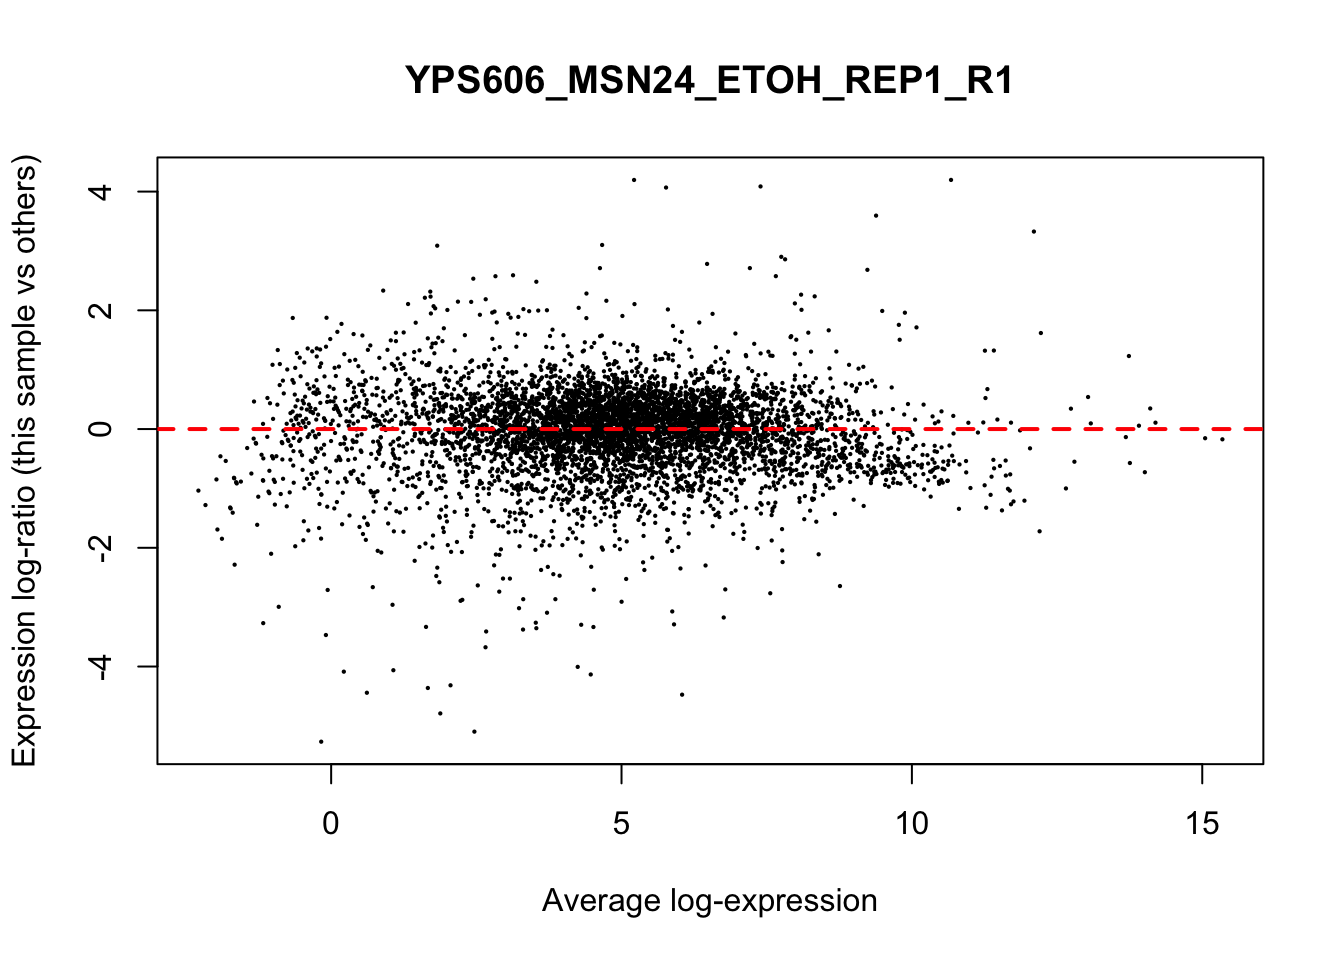
\includegraphics[width=0.25\linewidth]{_main_files/figure-latex/plotMDS-edgeR-1} 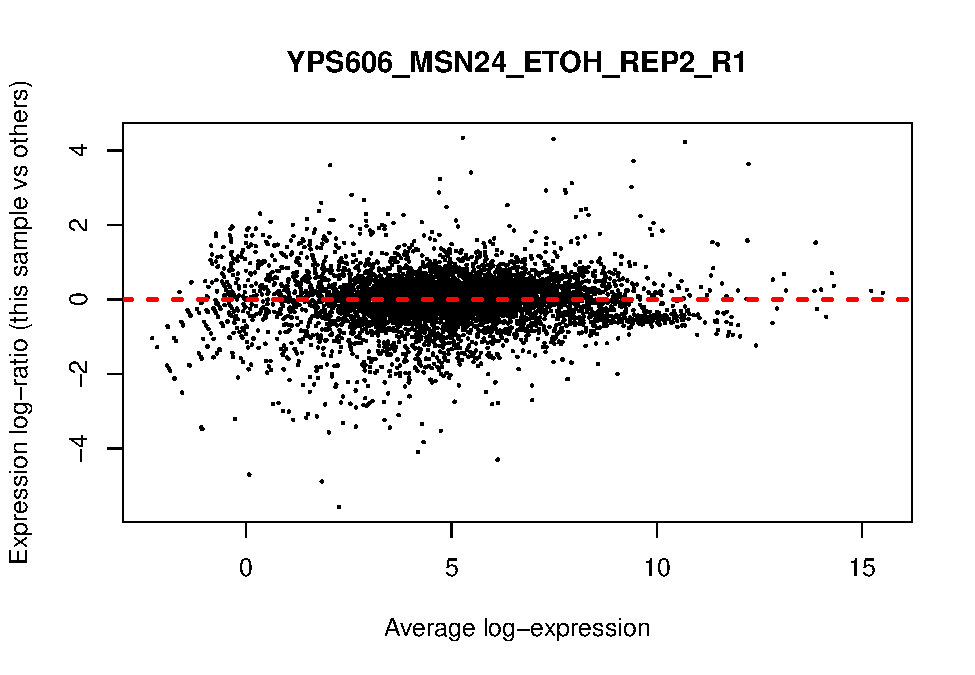
\includegraphics[width=0.25\linewidth]{_main_files/figure-latex/plotMDS-edgeR-2} 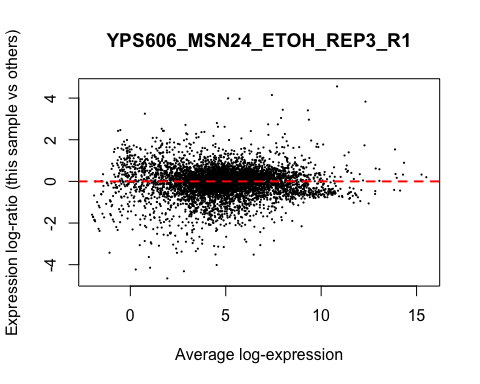
\includegraphics[width=0.25\linewidth]{_main_files/figure-latex/plotMDS-edgeR-3} 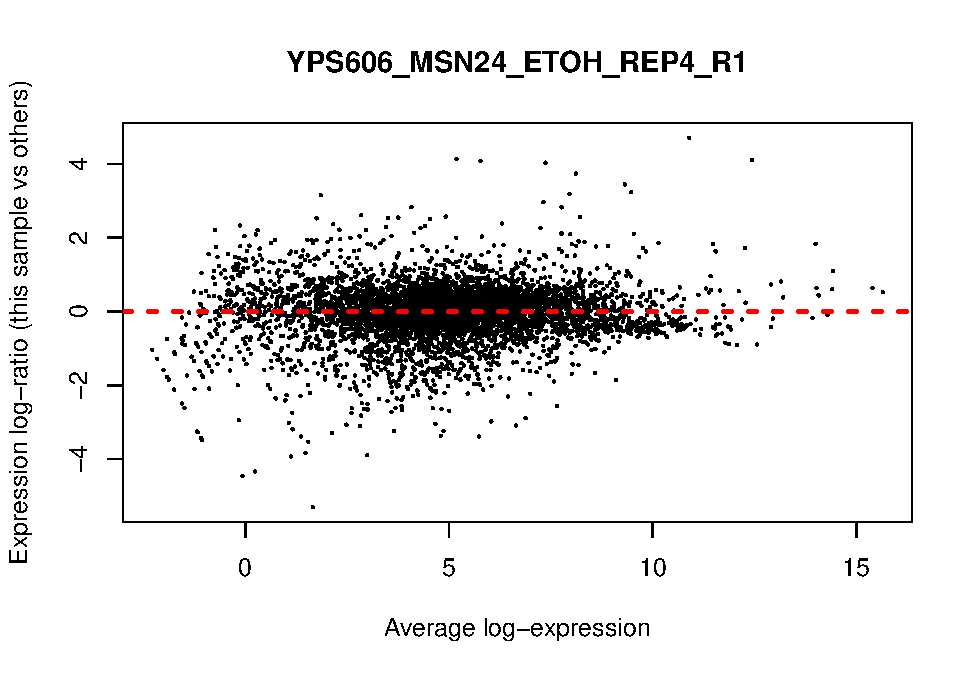
\includegraphics[width=0.25\linewidth]{_main_files/figure-latex/plotMDS-edgeR-4} 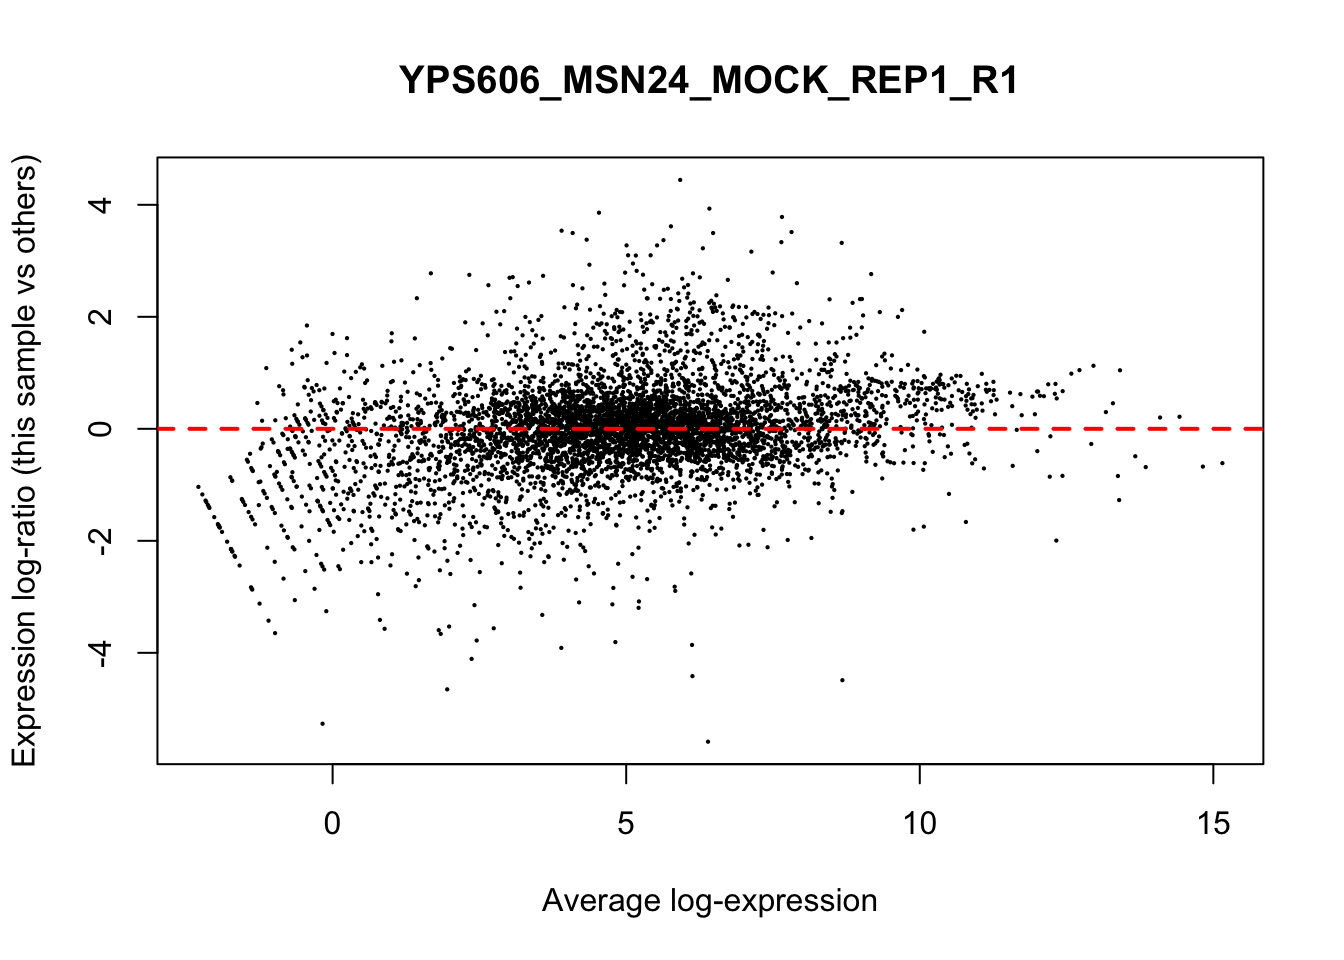
\includegraphics[width=0.25\linewidth]{_main_files/figure-latex/plotMDS-edgeR-5} 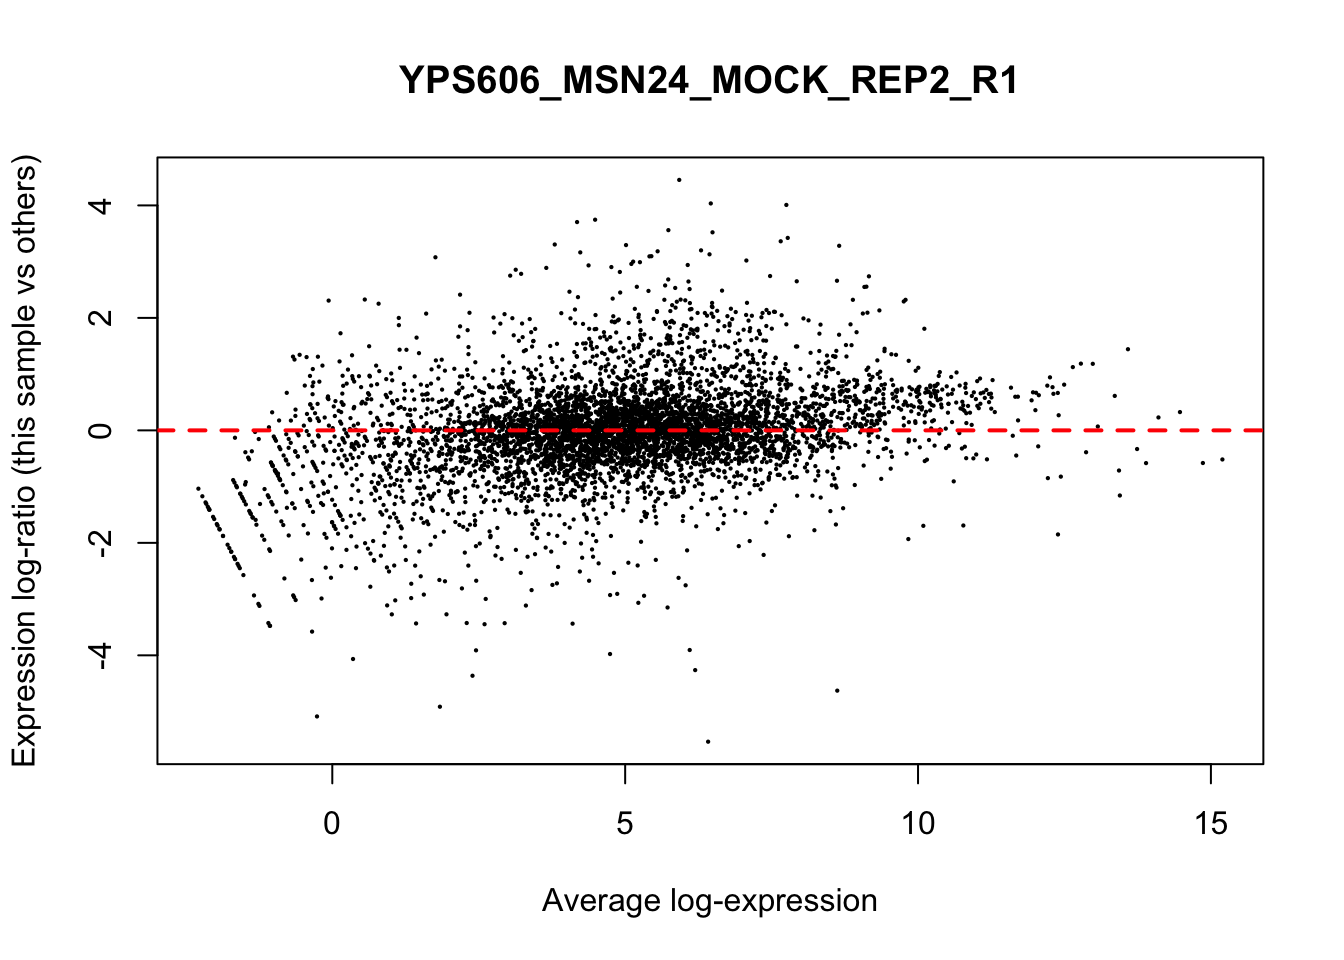
\includegraphics[width=0.25\linewidth]{_main_files/figure-latex/plotMDS-edgeR-6} 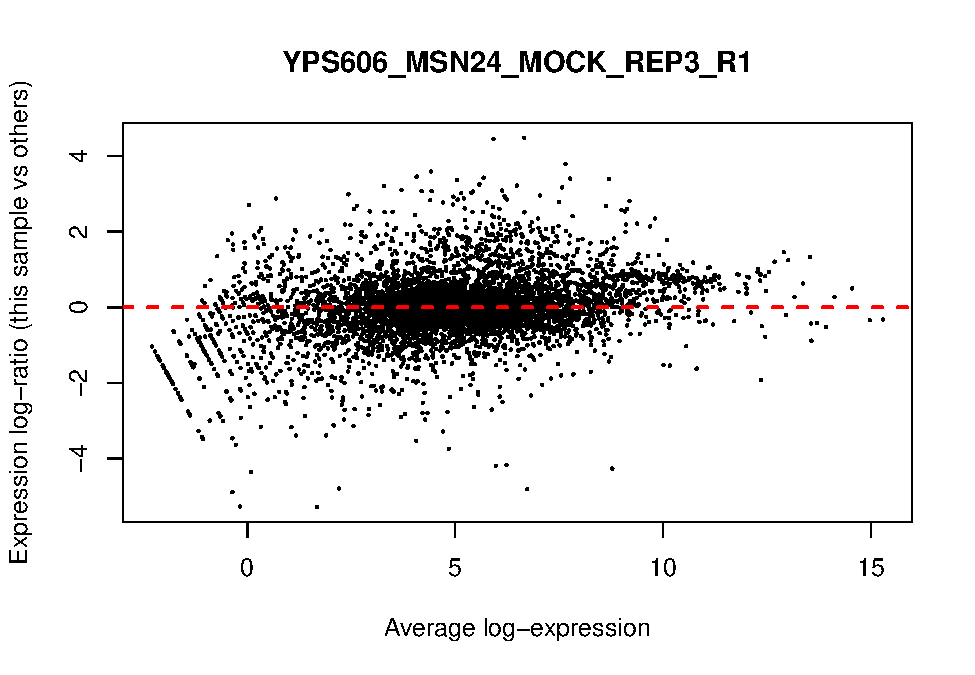
\includegraphics[width=0.25\linewidth]{_main_files/figure-latex/plotMDS-edgeR-7} 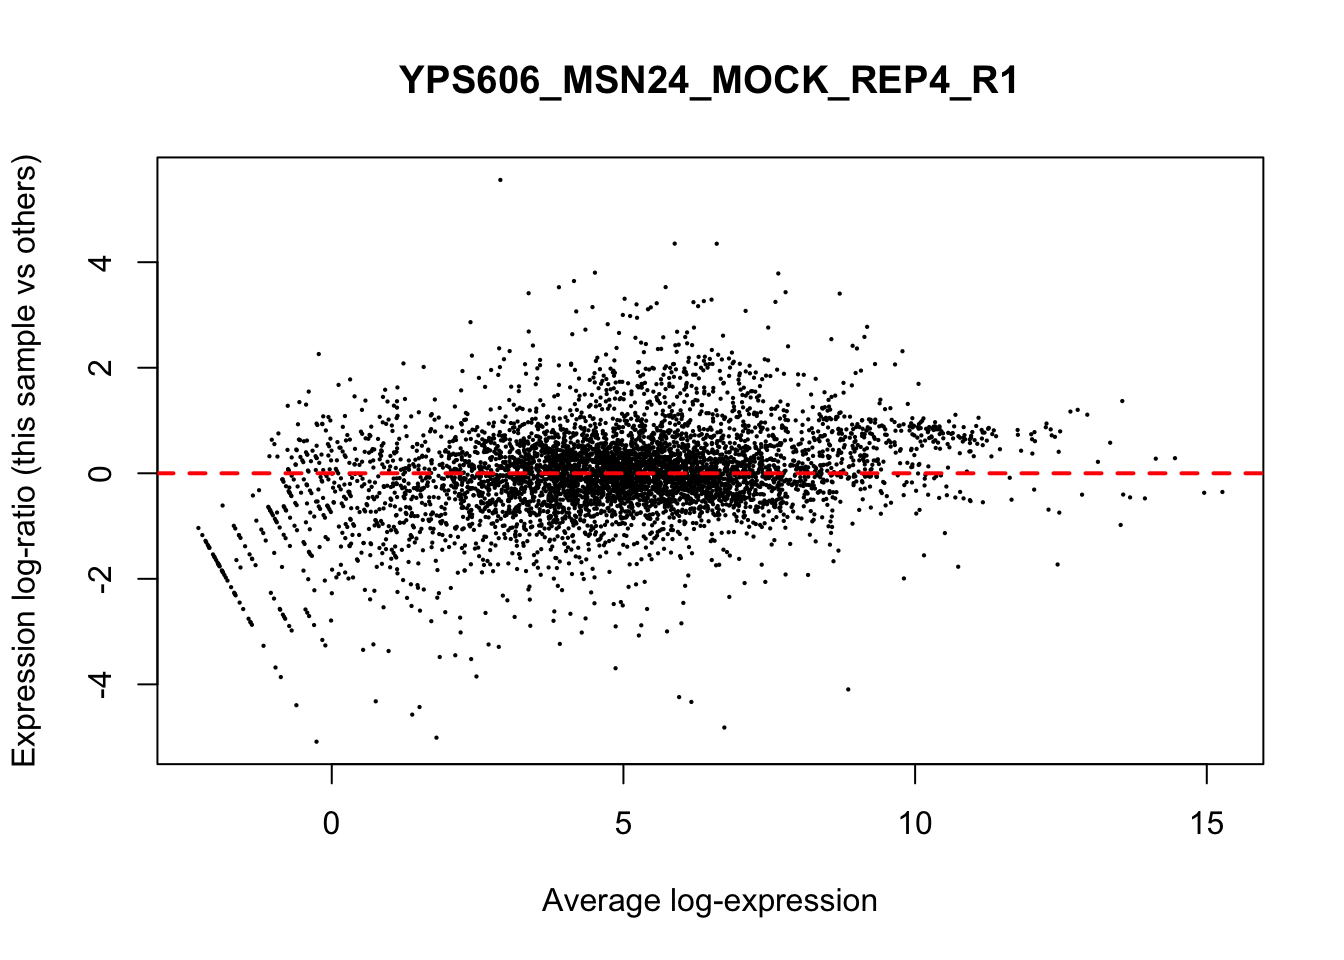
\includegraphics[width=0.25\linewidth]{_main_files/figure-latex/plotMDS-edgeR-8} 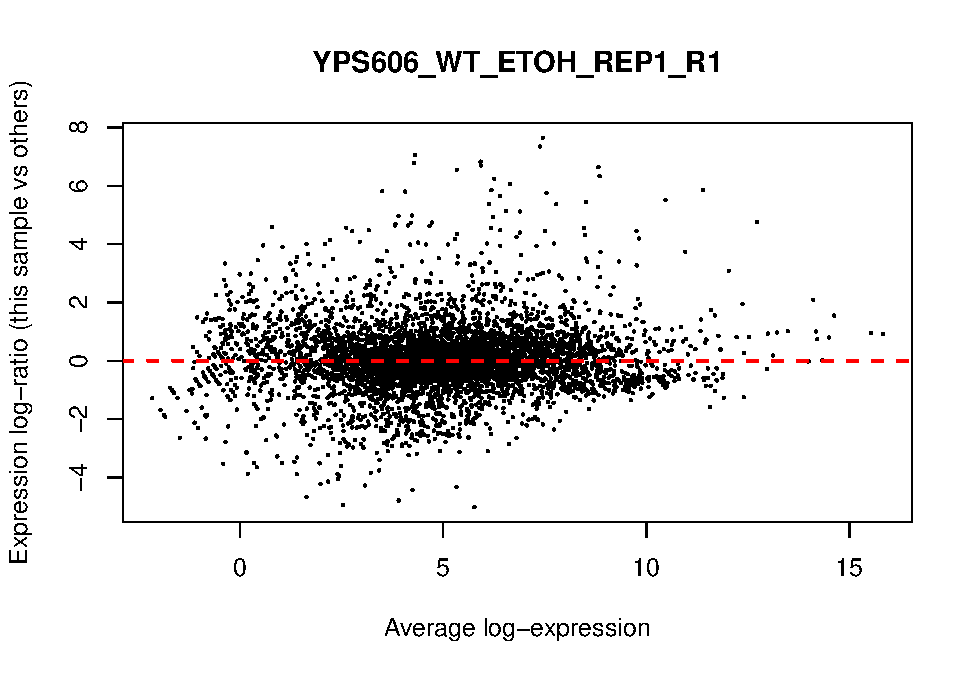
\includegraphics[width=0.25\linewidth]{_main_files/figure-latex/plotMDS-edgeR-9} 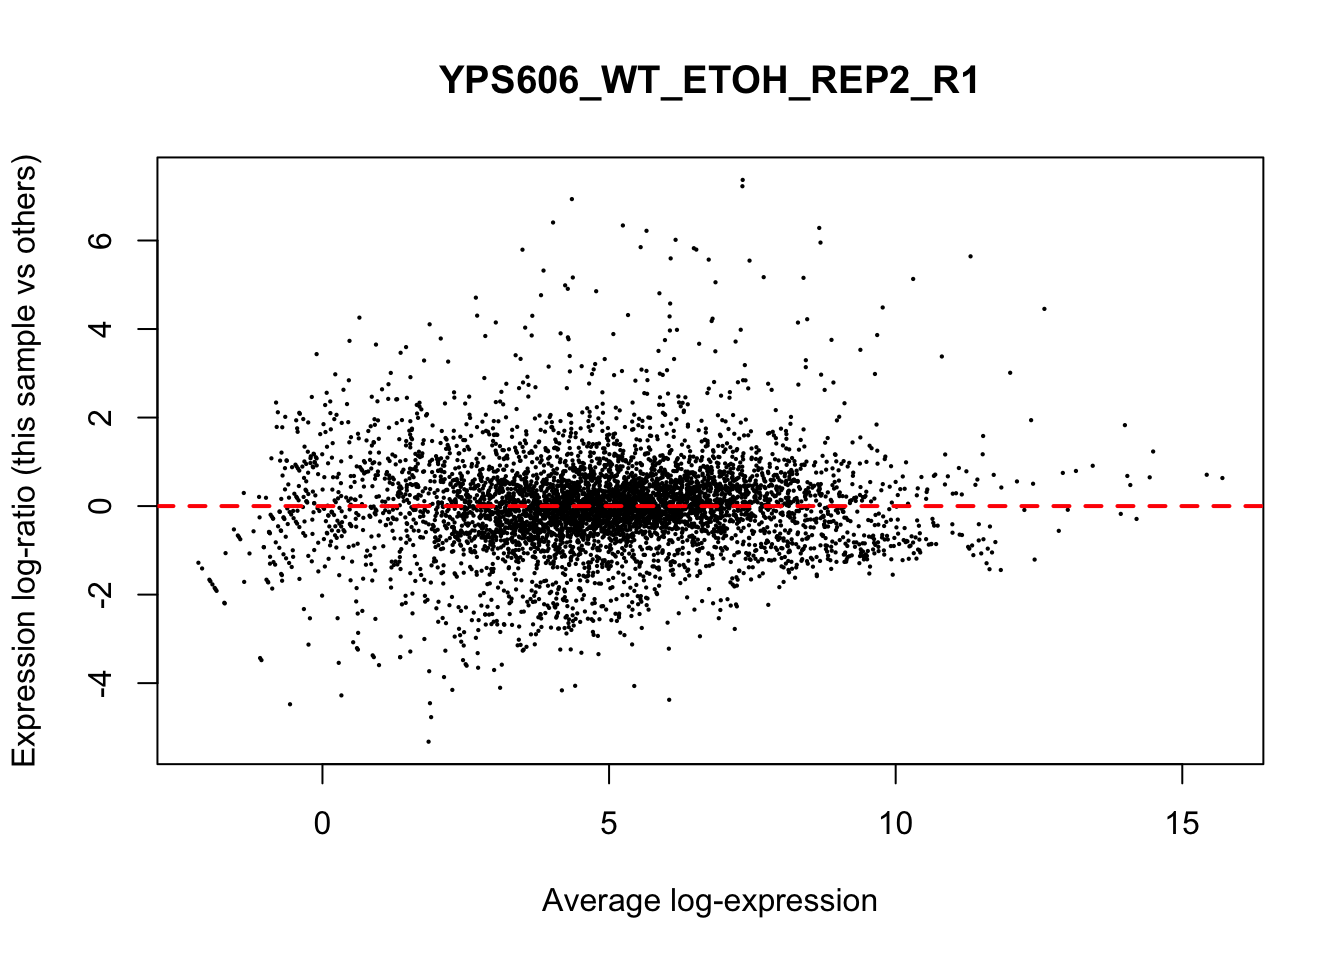
\includegraphics[width=0.25\linewidth]{_main_files/figure-latex/plotMDS-edgeR-10} 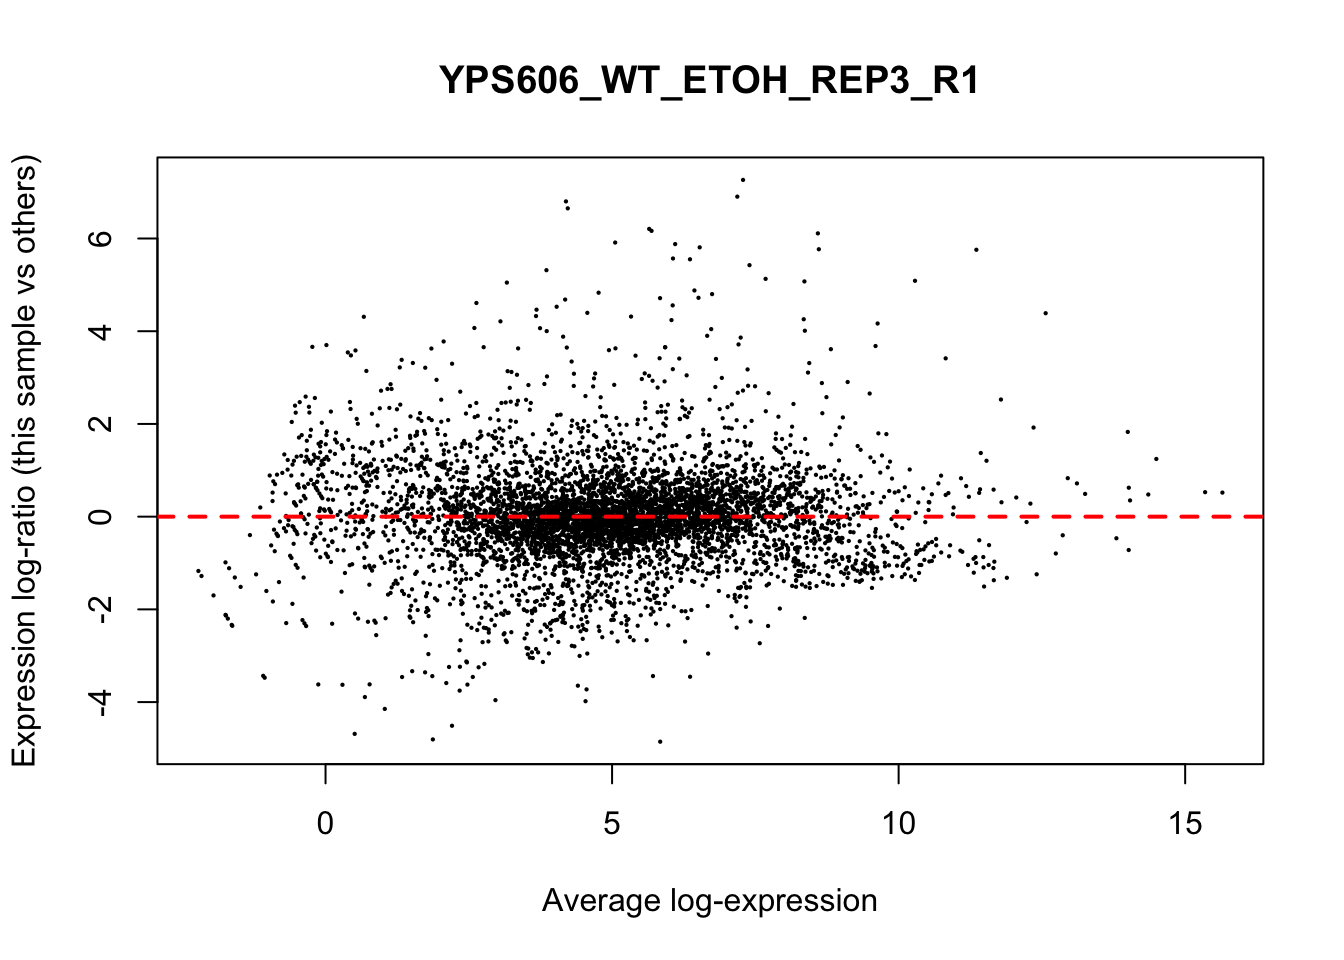
\includegraphics[width=0.25\linewidth]{_main_files/figure-latex/plotMDS-edgeR-11} 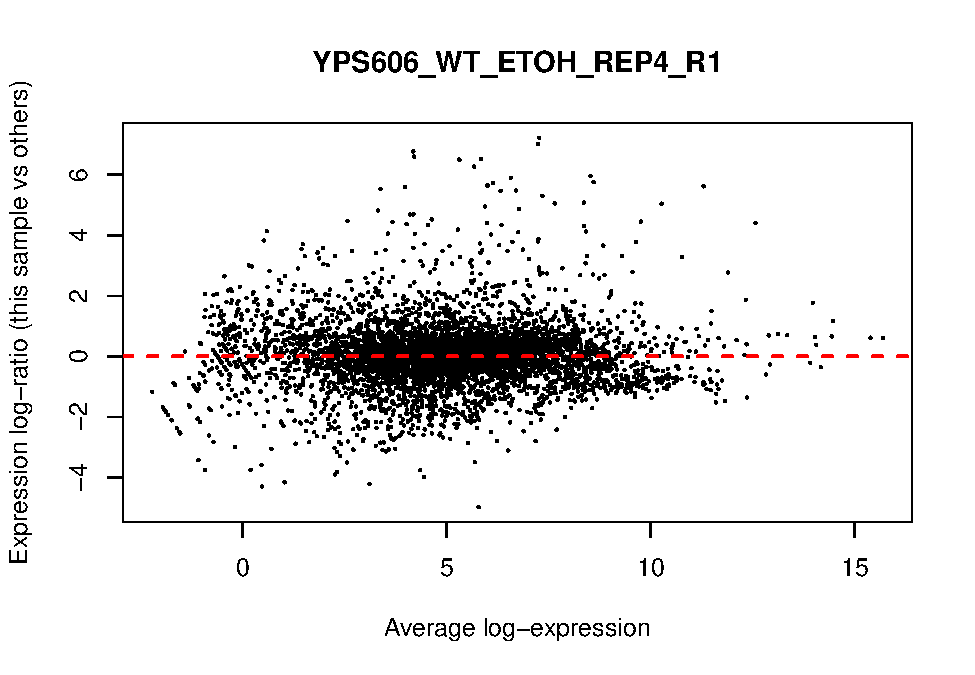
\includegraphics[width=0.25\linewidth]{_main_files/figure-latex/plotMDS-edgeR-12} 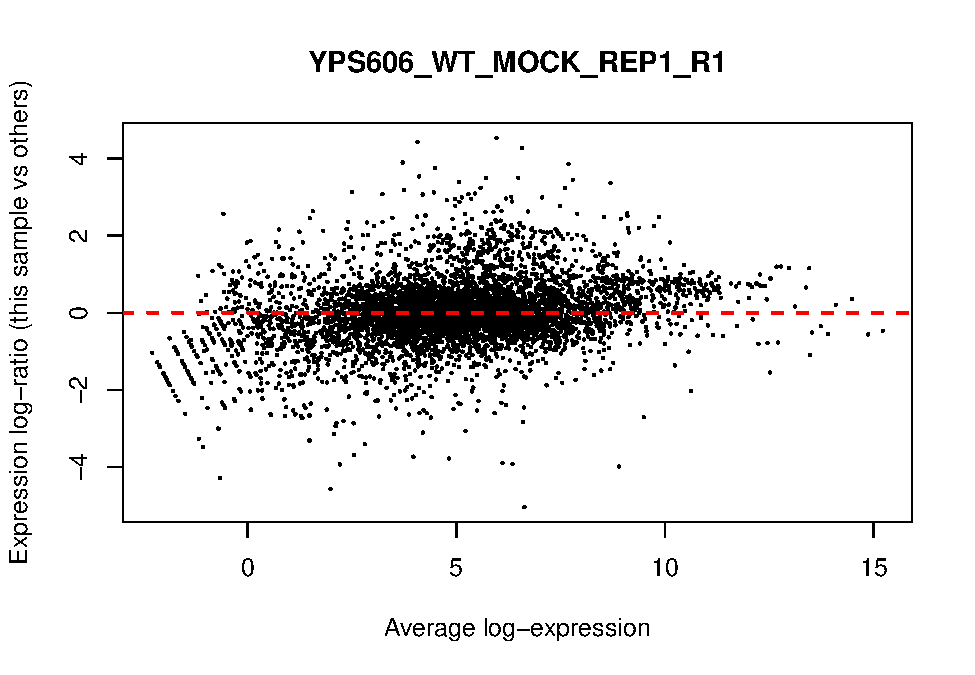
\includegraphics[width=0.25\linewidth]{_main_files/figure-latex/plotMDS-edgeR-13} 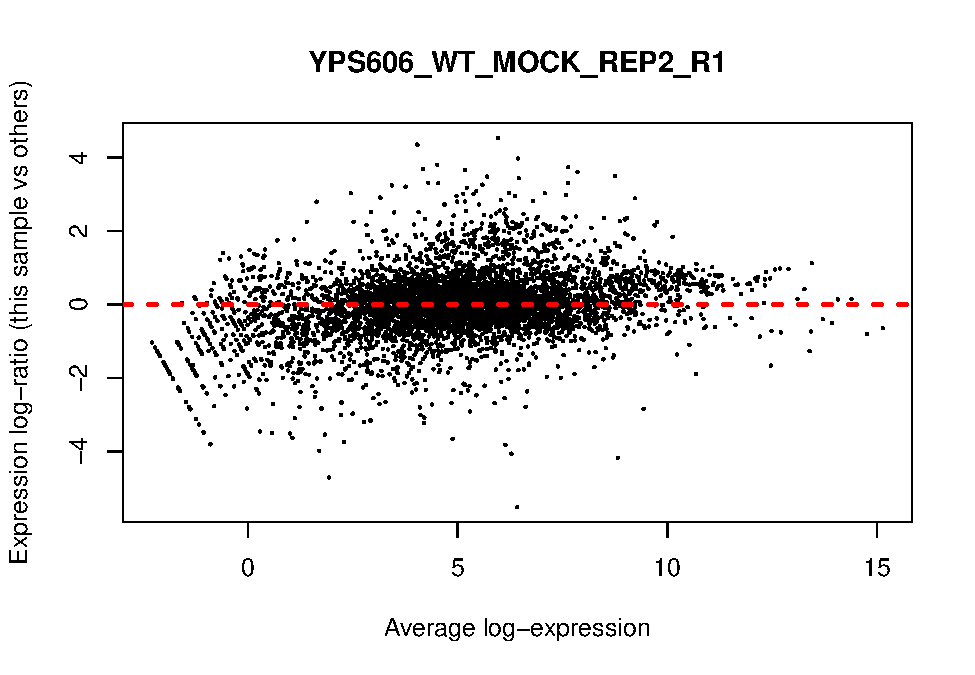
\includegraphics[width=0.25\linewidth]{_main_files/figure-latex/plotMDS-edgeR-14} 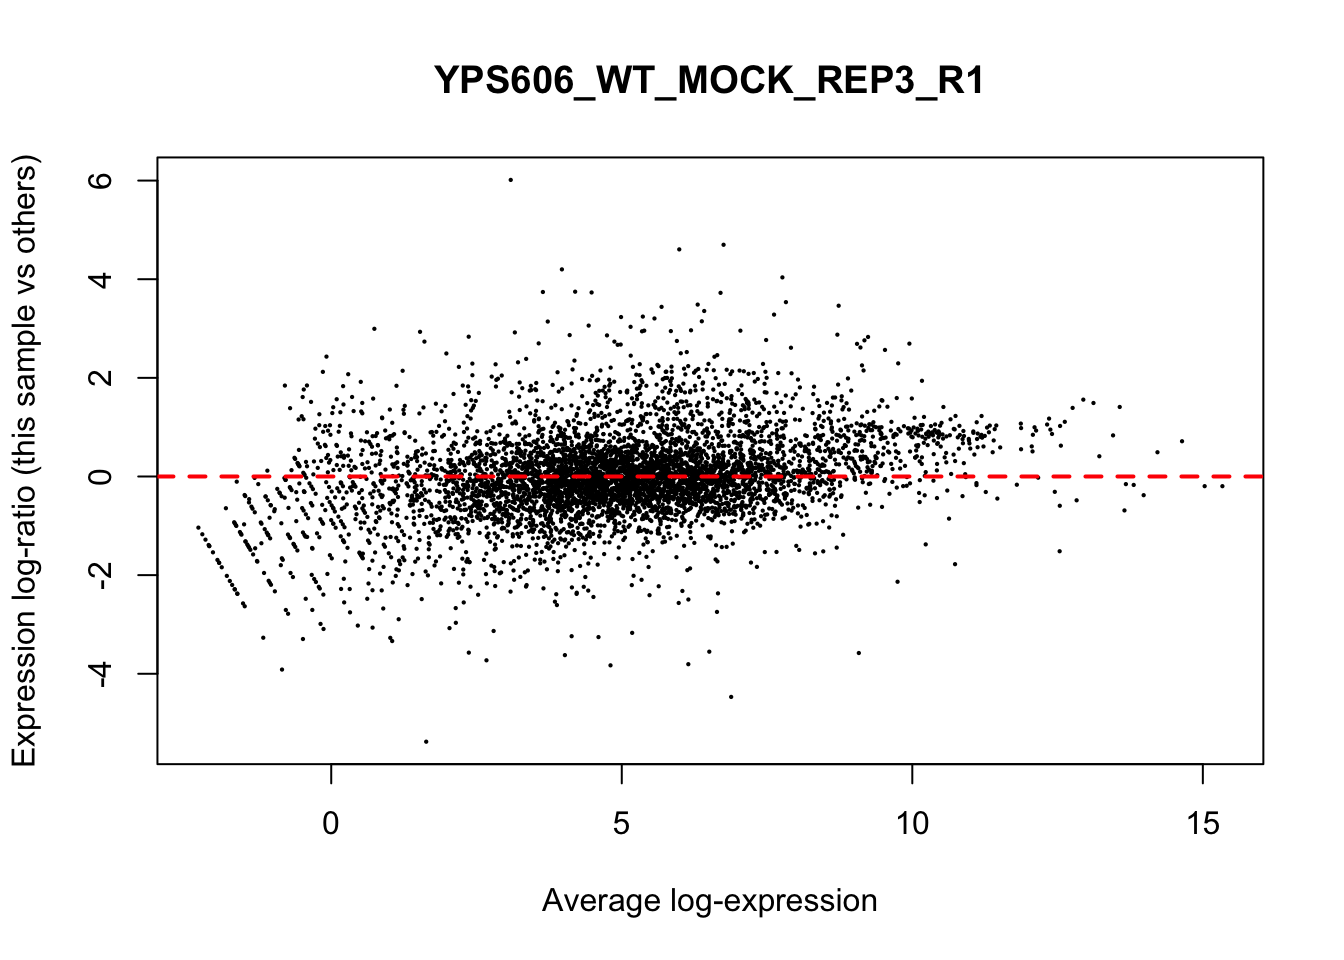
\includegraphics[width=0.25\linewidth]{_main_files/figure-latex/plotMDS-edgeR-15} 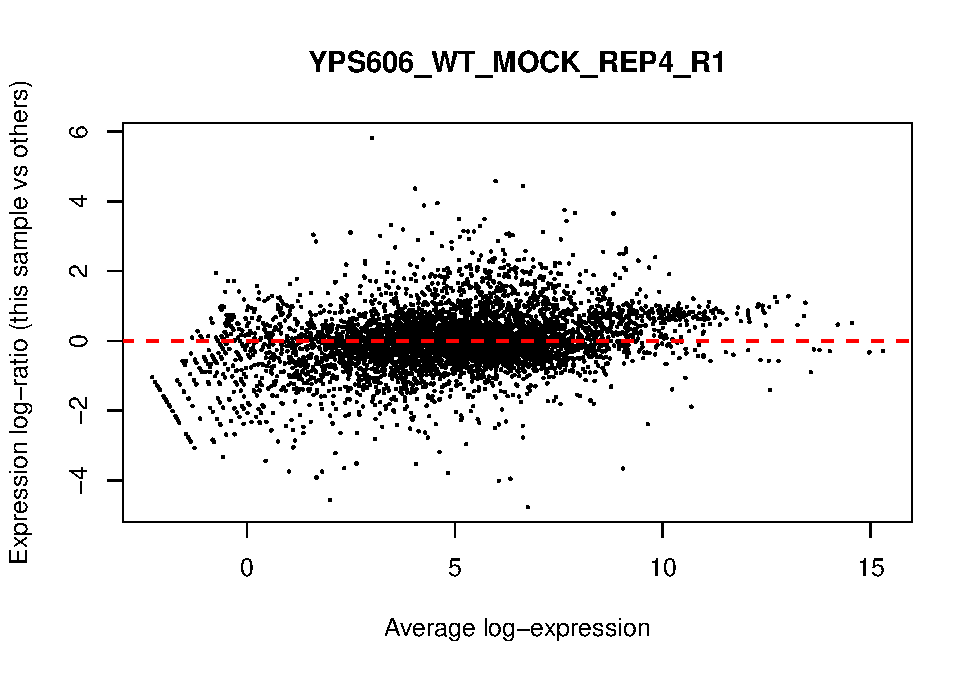
\includegraphics[width=0.25\linewidth]{_main_files/figure-latex/plotMDS-edgeR-16}

\hypertarget{exploring-differences-between-libraries}{%
\section{Exploring differences between libraries}\label{exploring-differences-between-libraries}}

The data can be explored by generating multi-dimensional scaling (MDS)
plots. This visualizes the differences between the expression profiles
of different samples in two dimensions. The next plot shows the MDS plot
for the yeast heatshock data.

\begin{Shaded}
\begin{Highlighting}[]
\NormalTok{points }\OtherTok{\textless{}{-}} \FunctionTok{c}\NormalTok{(}\DecValTok{1}\NormalTok{,}\DecValTok{1}\NormalTok{,}\DecValTok{2}\NormalTok{,}\DecValTok{2}\NormalTok{)}
\NormalTok{colors }\OtherTok{\textless{}{-}} \FunctionTok{rep}\NormalTok{(}\FunctionTok{c}\NormalTok{(}\StringTok{"black"}\NormalTok{, }\StringTok{"red"}\NormalTok{),}\DecValTok{8}\NormalTok{)}
\FunctionTok{plotMDS}\NormalTok{(y, }\AttributeTok{col=}\NormalTok{colors[group], }\AttributeTok{pch=}\NormalTok{points[group])}
\FunctionTok{legend}\NormalTok{(}\StringTok{"topright"}\NormalTok{, }\AttributeTok{legend=}\FunctionTok{levels}\NormalTok{(group),}
     \AttributeTok{pch=}\NormalTok{points, }\AttributeTok{col=}\NormalTok{colors, }\AttributeTok{ncol=}\DecValTok{2}\NormalTok{)}
\FunctionTok{title}\NormalTok{(}\AttributeTok{main=}\StringTok{"PCA plot"}\NormalTok{)}
\end{Highlighting}
\end{Shaded}

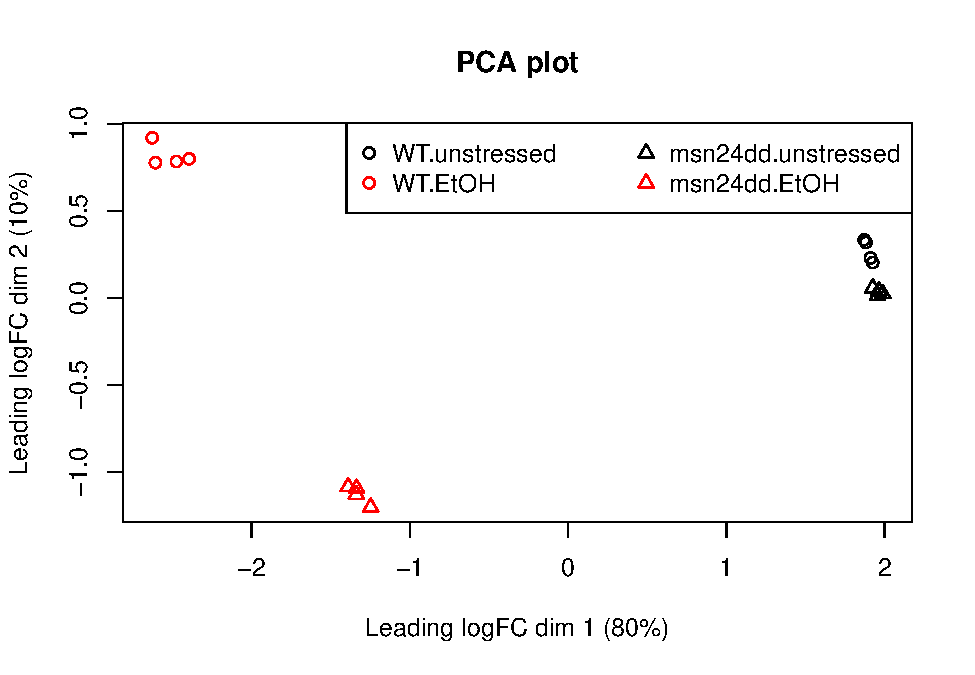
\includegraphics{_main_files/figure-latex/plot-MDS-edgeR-1.pdf}

\hypertarget{estimate-dispersion}{%
\section{Estimate Dispersion}\label{estimate-dispersion}}

The trended NB dispersion is estimated using the estimateDisp function.
This returns the DGEList object with additional entries for the
estimated NB dispersions for all genes. These estimates can be
visualized with plotBCV, which shows the root-estimate, i.e., the
biological coefficient of variation for each gene

\begin{Shaded}
\begin{Highlighting}[]
\NormalTok{y }\OtherTok{\textless{}{-}} \FunctionTok{estimateDisp}\NormalTok{(y, design, }\AttributeTok{robust=}\ConstantTok{TRUE}\NormalTok{)}
\FunctionTok{plotBCV}\NormalTok{(y)}
\FunctionTok{title}\NormalTok{(}\AttributeTok{main=}\StringTok{"Biological Coefficient of Variation (BCV) vs gene abundance"}\NormalTok{)}
\end{Highlighting}
\end{Shaded}

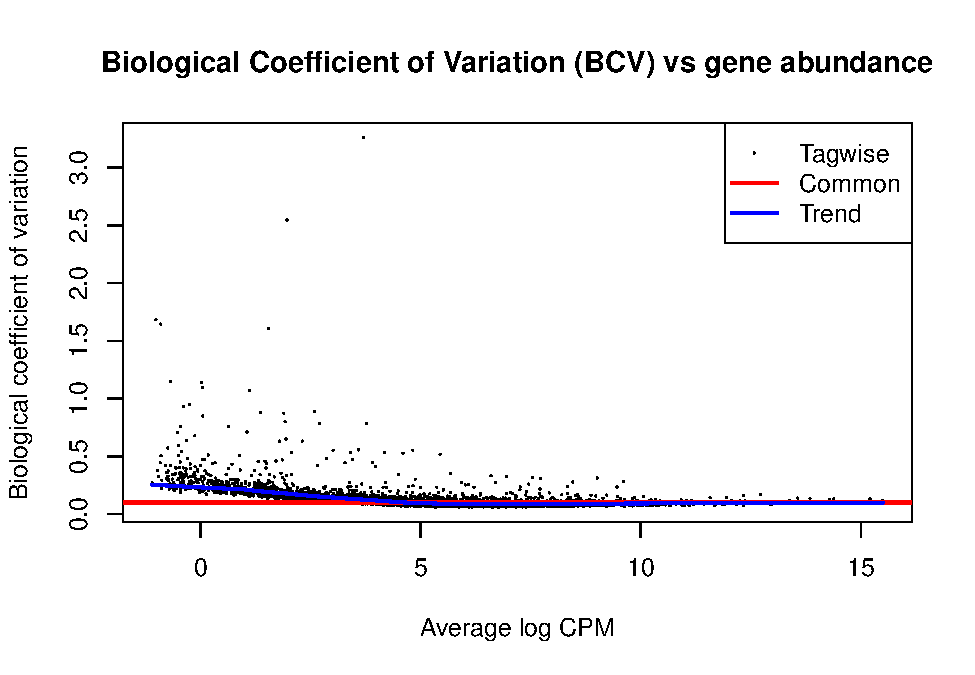
\includegraphics{_main_files/figure-latex/estimate-dispersion-edgeR-1.pdf}

In general, the trend in the NB dispersions should decrease smoothly
with increasing abundance. This is because the expression of
high-abundance genes is expected to be more stable than that of
low-abundance genes. Any substantial increase at high abundances may be
indicative of batch effects or trended biases. The value of the trended
NB dispersions should range between 0.005 to 0.05 for
laboratory-controlled biological systems like mice or cell lines, though
larger values will be observed for patient-derived data (\textgreater{} 0.1)

For the QL dispersions, estimation can be performed using the glmQLFit
function. This returns a DGEGLM object containing the estimated values
of the GLM coefficients for each gene

\begin{Shaded}
\begin{Highlighting}[]
\NormalTok{fit }\OtherTok{\textless{}{-}} \FunctionTok{glmQLFit}\NormalTok{(y, design, }\AttributeTok{robust=}\ConstantTok{TRUE}\NormalTok{)}
\FunctionTok{head}\NormalTok{(fit}\SpecialCharTok{$}\NormalTok{coefficients)}
\end{Highlighting}
\end{Shaded}

\begin{verbatim}
##         WT.unstressed WT.EtOH msn24dd.unstressed msn24dd.EtOH
## YIL170W         -15.1  -13.10             -15.87       -13.21
## YFL056C         -11.1  -11.01             -11.07       -10.42
## YAR061W         -13.7  -13.30             -13.36       -13.36
## YGR014W          -8.5   -8.74              -8.41        -8.66
## YPR031W         -10.5  -11.89             -10.45       -11.86
## YIL003W         -10.6  -12.07             -10.72       -11.97
\end{verbatim}

\begin{Shaded}
\begin{Highlighting}[]
\FunctionTok{plotQLDisp}\NormalTok{(fit)}
\FunctionTok{title}\NormalTok{(}\AttributeTok{main=}\StringTok{"QL Dispersion of the fit"}\NormalTok{)}
\end{Highlighting}
\end{Shaded}

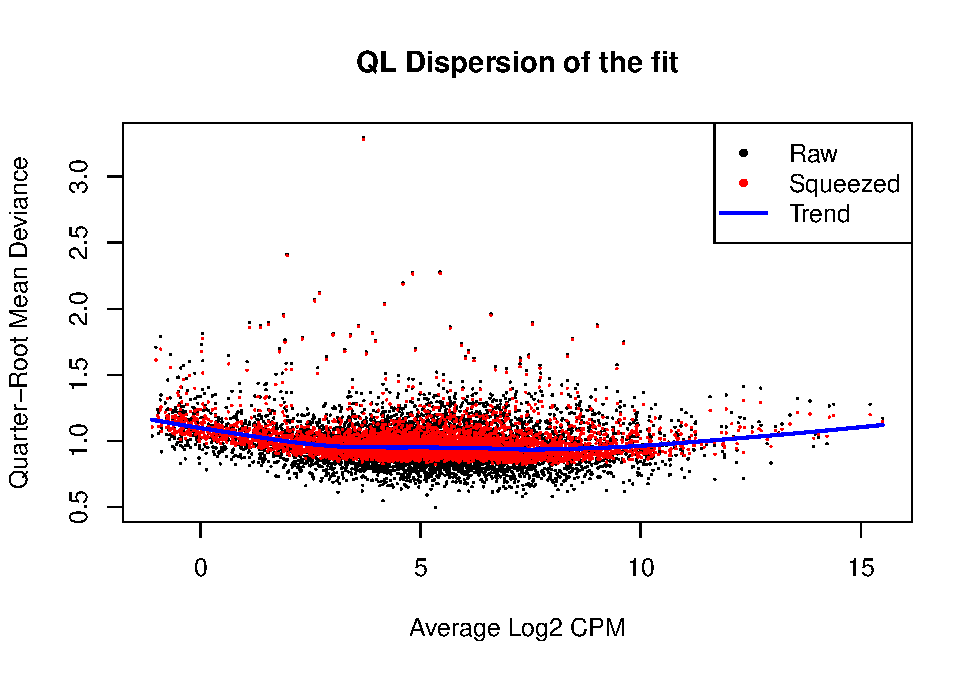
\includegraphics{_main_files/figure-latex/generate-fit-edgeR-1.pdf}

EB squeezing of the raw dispersion estimators towards the trend reduces
the uncertainty of the final estimators. The extent of this moderation
is determined by the value of the prior df, as estimated from the data.
Large estimates for the prior df indicate that the QL dispersions are
less variable between genes, meaning that stronger EB moderation can be
performed. Small values for the prior df indicate that the dispersions
are highly variable, meaning that strong moderation would be
inappropriate

Setting \texttt{robust=TRUE} in glmQLFit is strongly recommended. This causes
glmQLFit to estimate a vector of df.prior values, with lower values for
outlier genes and larger values for the main body of genes.

\hypertarget{testing-for-differential-expression}{%
\section{Testing for differential expression}\label{testing-for-differential-expression}}

The final step is to actually test for significant differential
expression in each gene, using the QL F-test. The contrast of interest
can be specified using the makeContrasts function. Here, genes are
detected that are DE between the stressed and unstressed. This is done
by defining the null hypothesis as heat stressed - unstressed = 0.

\begin{Shaded}
\begin{Highlighting}[]
\CommentTok{\# generate contrasts we are interested in learning about}
\NormalTok{my.contrasts }\OtherTok{\textless{}{-}} \FunctionTok{makeContrasts}\NormalTok{(}\AttributeTok{EtOHvsMOCK.WT =}\NormalTok{ WT.EtOH }\SpecialCharTok{{-}}\NormalTok{ WT.unstressed, }
                     \AttributeTok{EtOHvsMOCK.MSN24dd =}\NormalTok{ msn24dd.EtOH }\SpecialCharTok{{-}}\NormalTok{ msn24dd.unstressed,}
                     \AttributeTok{EtOH.MSN24ddvsWT =}\NormalTok{ msn24dd.EtOH }\SpecialCharTok{{-}}\NormalTok{ WT.EtOH,}
                     \AttributeTok{MOCK.MSN24ddvsWT =}\NormalTok{ msn24dd.unstressed }\SpecialCharTok{{-}}\NormalTok{ WT.unstressed,}
                     \AttributeTok{EtOHvsWT.MSN24ddvsWT =}\NormalTok{ (msn24dd.EtOH}\SpecialCharTok{{-}}\NormalTok{msn24dd.unstressed)}\SpecialCharTok{{-}}\NormalTok{(WT.EtOH}\SpecialCharTok{{-}}\NormalTok{WT.unstressed),}
                     \AttributeTok{levels=}\NormalTok{design)}

\CommentTok{\# This contrast looks at the difference in the stress responses between mutant and WT}
\NormalTok{res }\OtherTok{\textless{}{-}} \FunctionTok{glmQLFTest}\NormalTok{(fit, }\AttributeTok{contrast =}\NormalTok{ my.contrasts[,}\StringTok{"EtOHvsWT.MSN24ddvsWT"}\NormalTok{])}
\end{Highlighting}
\end{Shaded}

\begin{Shaded}
\begin{Highlighting}[]
\CommentTok{\# let\textquotesingle{}s take a quick look at the results}
\FunctionTok{topTags}\NormalTok{(res, }\AttributeTok{n=}\DecValTok{10}\NormalTok{) }
\end{Highlighting}
\end{Shaded}

\begin{verbatim}
## Coefficient:  1*WT.unstressed -1*WT.EtOH -1*msn24dd.unstressed 1*msn24dd.EtOH 
##             ORF        SGD GENENAME logFC logCPM    F   PValue      FDR
## YMR105C YMR105C S000004711     PGM2 -6.84   9.70 1608 2.91e-24 1.64e-20
## YMR196W YMR196W S000004809     <NA> -5.15   8.36  877 5.58e-21 1.06e-17
## YKL035W YKL035W S000001518     UGP1 -3.84  10.78  868 5.65e-21 1.06e-17
## YDR516C YDR516C S000002924     EMI2 -4.01   9.08  795 1.65e-20 2.31e-17
## YBR126C YBR126C S000000330     TPS1 -3.46   9.81  693 8.80e-20 9.32e-17
## YLR258W YLR258W S000004248     GSY2 -4.86   8.25  680 1.10e-19 9.32e-17
## YPR149W YPR149W S000006353   NCE102 -4.24   7.95  790 1.16e-19 9.32e-17
## YDR001C YDR001C S000002408     NTH1 -2.89   7.08  650 1.89e-19 1.33e-16
## YHL021C YHL021C S000001013    AIM17 -4.21   6.88  635 3.51e-19 2.19e-16
## YML100W YML100W S000004566     TSL1 -7.12   9.81 1003 5.62e-19 3.15e-16
\end{verbatim}

\begin{Shaded}
\begin{Highlighting}[]
\CommentTok{\# generate a beautiful table for the pdf/html file.}
\FunctionTok{topTags}\NormalTok{(res, }\AttributeTok{n=}\ConstantTok{Inf}\NormalTok{) }\SpecialCharTok{|\textgreater{}} \FunctionTok{data.frame}\NormalTok{() }\SpecialCharTok{|\textgreater{}} 
  \FunctionTok{arrange}\NormalTok{(FDR) }\SpecialCharTok{|\textgreater{}}
  \FunctionTok{mutate}\NormalTok{(}\AttributeTok{logFC=}\FunctionTok{round}\NormalTok{(logFC,}\DecValTok{2}\NormalTok{)) }\SpecialCharTok{|\textgreater{}}
  \CommentTok{\# mutate(across(where(is.numeric), signif, 3)) |\textgreater{}}
  \FunctionTok{mutate\_if}\NormalTok{(is.numeric, signif, }\DecValTok{3}\NormalTok{) }\SpecialCharTok{|\textgreater{}}
  \FunctionTok{remove\_rownames}\NormalTok{() }\SpecialCharTok{|\textgreater{}}
  \FunctionTok{reactable}\NormalTok{(}
    \AttributeTok{searchable =} \ConstantTok{TRUE}\NormalTok{,}
    \AttributeTok{showSortable =} \ConstantTok{TRUE}\NormalTok{,}
    \AttributeTok{columns =} \FunctionTok{list}\NormalTok{(}\AttributeTok{ORF =} \FunctionTok{colDef}\NormalTok{(}
      \AttributeTok{cell =} \ControlFlowTok{function}\NormalTok{(value) \{}
        \CommentTok{\# Render as a link}
\NormalTok{        url }\OtherTok{\textless{}{-}}
          \FunctionTok{sprintf}\NormalTok{(}\StringTok{"https://www.yeastgenome.org/locus/\%s"}\NormalTok{, value)}
\NormalTok{        htmltools}\SpecialCharTok{::}\NormalTok{tags}\SpecialCharTok{$}\FunctionTok{a}\NormalTok{(}\AttributeTok{href =}\NormalTok{ url, }\AttributeTok{target =} \StringTok{"\_blank"}\NormalTok{, }\FunctionTok{as.character}\NormalTok{(value))}
\NormalTok{      \}}
\NormalTok{    ))}
\NormalTok{  )}
\end{Highlighting}
\end{Shaded}

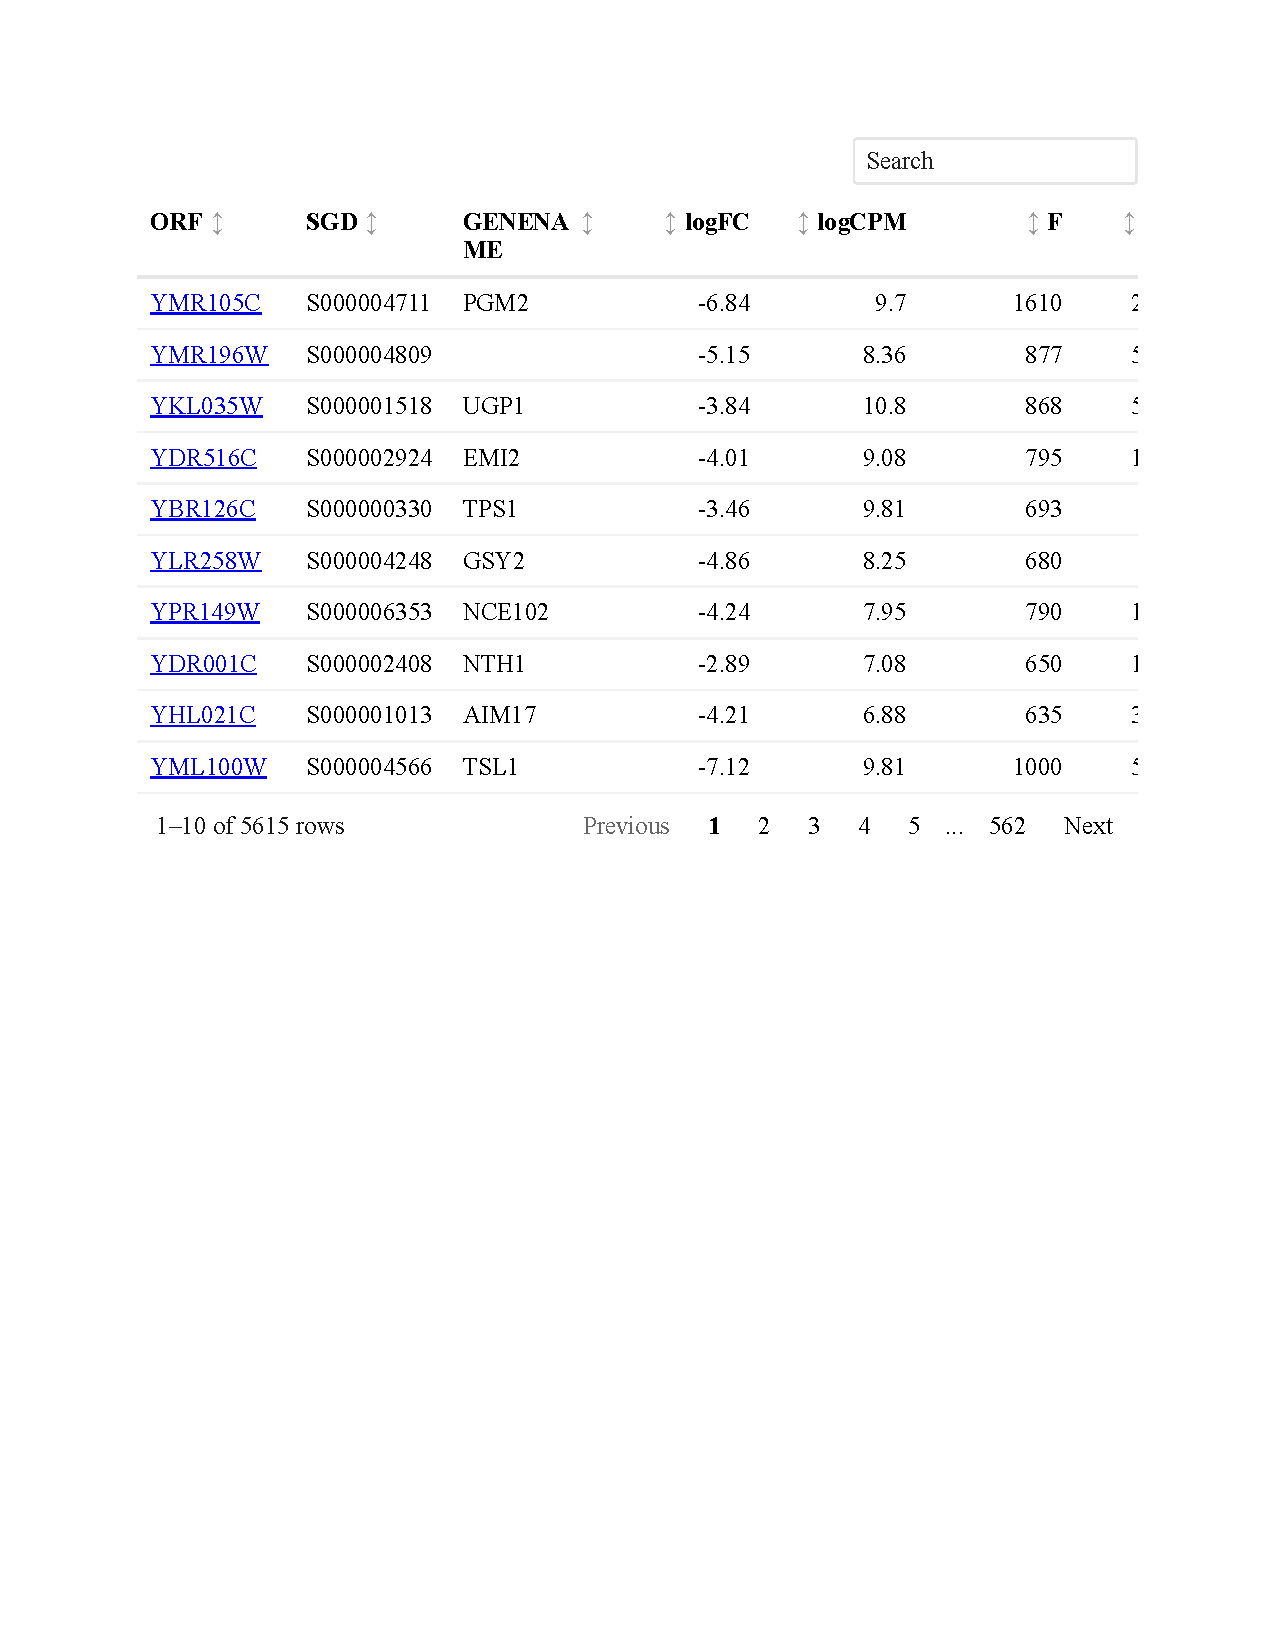
\includegraphics{_main_files/figure-latex/create-Table-edgeR-1.pdf}

\begin{Shaded}
\begin{Highlighting}[]
\NormalTok{is.de }\OtherTok{\textless{}{-}} \FunctionTok{decideTestsDGE}\NormalTok{(res, }
                        \AttributeTok{p.value=}\FloatTok{0.05}\NormalTok{,}
                        \AttributeTok{lfc =} \DecValTok{0}\NormalTok{) }\CommentTok{\# this allows you to set a cutoff, BUT...}
\CommentTok{\# if you want to compare against a FC that isn\textquotesingle{}t 0, should use glmTreat instead.}

\FunctionTok{summary}\NormalTok{(is.de)}
\end{Highlighting}
\end{Shaded}

\begin{verbatim}
##        1*WT.unstressed -1*WT.EtOH -1*msn24dd.unstressed 1*msn24dd.EtOH
## Down                                                               761
## NotSig                                                            4031
## Up                                                                 823
\end{verbatim}

Let's take a quick look at the differential expression

\begin{Shaded}
\begin{Highlighting}[]
\FunctionTok{plotSmear}\NormalTok{(res, }\AttributeTok{de.tags=}\FunctionTok{rownames}\NormalTok{(res)[is.de}\SpecialCharTok{!=}\DecValTok{0}\NormalTok{])}
\FunctionTok{title}\NormalTok{(}\AttributeTok{main=}\StringTok{"DE genes using glmQLFTest, FDR\textless{}0.05"}\NormalTok{)}
\end{Highlighting}
\end{Shaded}

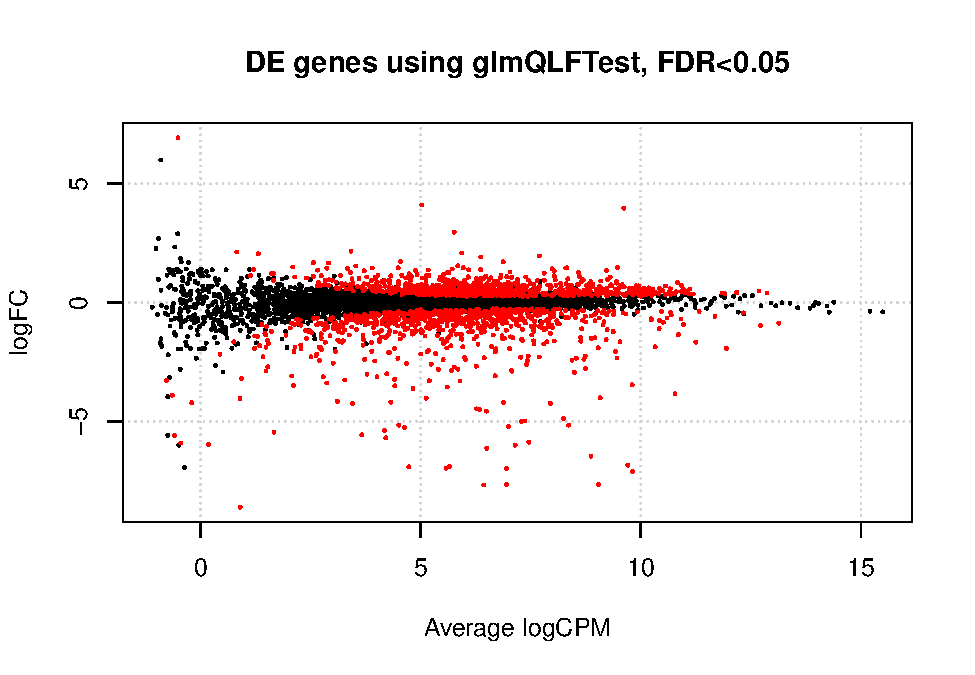
\includegraphics{_main_files/figure-latex/visualize-DEgenes-edgeR-1.pdf}

Here is how we can save our output file(s).

\begin{Shaded}
\begin{Highlighting}[]
\CommentTok{\# Choose topTags destination}
\NormalTok{dir\_output\_edgeR }\OtherTok{\textless{}{-}}
  \FunctionTok{path.expand}\NormalTok{(}\StringTok{"\textasciitilde{}/Desktop/Genomic\_Data\_Analysis/Analysis/edgeR/"}\NormalTok{)}
\ControlFlowTok{if}\NormalTok{ (}\SpecialCharTok{!}\FunctionTok{dir.exists}\NormalTok{(dir\_output\_edgeR)) \{}
  \FunctionTok{dir.create}\NormalTok{(dir\_output\_edgeR, }\AttributeTok{recursive =} \ConstantTok{TRUE}\NormalTok{)}
\NormalTok{\}}

\CommentTok{\# for shairng with others, the topTags output is convenient.}
\FunctionTok{topTags}\NormalTok{(res, }\AttributeTok{n =} \ConstantTok{Inf}\NormalTok{) }\SpecialCharTok{|\textgreater{}} \FunctionTok{data.frame}\NormalTok{() }\SpecialCharTok{|\textgreater{}}
  \FunctionTok{arrange}\NormalTok{(}\FunctionTok{desc}\NormalTok{(logFC)) }\SpecialCharTok{|\textgreater{}}
  \FunctionTok{mutate}\NormalTok{(}\AttributeTok{logFC =} \FunctionTok{round}\NormalTok{(logFC, }\DecValTok{2}\NormalTok{)) }\SpecialCharTok{|\textgreater{}}
  \CommentTok{\# mutate(across(where(is.numeric), signif, 3)) |\textgreater{}}
  \FunctionTok{mutate\_if}\NormalTok{(is.numeric, signif, }\DecValTok{3}\NormalTok{) }\SpecialCharTok{|\textgreater{}}
  \FunctionTok{write\_tsv}\NormalTok{(}\AttributeTok{x=}\NormalTok{\_, }\AttributeTok{file =} \FunctionTok{paste0}\NormalTok{(dir\_output\_edgeR, }\StringTok{"yeast\_topTags\_edgeR.tsv"}\NormalTok{))}

\CommentTok{\# for subsequent analysis, let\textquotesingle{}s save the res object as an R data object.}
\FunctionTok{saveRDS}\NormalTok{(}\AttributeTok{object =}\NormalTok{ res, }\AttributeTok{file =} \FunctionTok{paste0}\NormalTok{(dir\_output\_edgeR, }\StringTok{"yeast\_res\_edgeR.Rds"}\NormalTok{))}

\CommentTok{\# we might also want our y object list}
\FunctionTok{saveRDS}\NormalTok{(}\AttributeTok{object =}\NormalTok{ y, }\AttributeTok{file =} \FunctionTok{paste0}\NormalTok{(dir\_output\_edgeR, }\StringTok{"yeast\_y\_edgeR.Rds"}\NormalTok{))}
\end{Highlighting}
\end{Shaded}

\hypertarget{looking-at-all-contrasts-at-once}{%
\section{Looking at all contrasts at once}\label{looking-at-all-contrasts-at-once}}

If we want results from all contrasts, we need to loop through them in edgeR, and them combine the results We will look more at the results of this in a later activity.

\begin{Shaded}
\begin{Highlighting}[]
\CommentTok{\# One way is to not specify just one contrast, like this:}
\NormalTok{res\_all }\OtherTok{\textless{}{-}} \FunctionTok{glmQLFTest}\NormalTok{(fit, }\AttributeTok{contrast =}\NormalTok{ my.contrasts)}

\NormalTok{res\_all }\SpecialCharTok{|\textgreater{}} 
  \FunctionTok{topTags}\NormalTok{(}\AttributeTok{n=}\ConstantTok{Inf}\NormalTok{) }\SpecialCharTok{|\textgreater{}} 
  \FunctionTok{data.frame}\NormalTok{() }\SpecialCharTok{|\textgreater{}}
  \FunctionTok{head}\NormalTok{()}
\end{Highlighting}
\end{Shaded}

\begin{verbatim}
##             ORF        SGD GENENAME logFC.EtOHvsMOCK.WT
## YDR516C YDR516C S000002924     EMI2                7.04
## YGR008C YGR008C S000003240     STF2                7.23
## YNL141W YNL141W S000005085     AAH1               -8.23
## YLR258W YLR258W S000004248     GSY2                7.56
## YMR105C YMR105C S000004711     PGM2                7.63
## YER103W YER103W S000000905     SSA4                7.77
##         logFC.EtOHvsMOCK.MSN24dd logFC.EtOH.MSN24ddvsWT logFC.MOCK.MSN24ddvsWT
## YDR516C                    3.030                 -4.717                 -0.710
## YGR008C                    2.020                 -6.118                 -0.906
## YNL141W                   -9.064                 -0.971                 -0.133
## YLR258W                    2.692                 -5.239                 -0.376
## YMR105C                    0.794                 -6.981                 -0.140
## YER103W                    7.122                 -0.796                 -0.149
##         logFC.EtOHvsWT.MSN24ddvsWT logCPM    F   PValue      FDR
## YDR516C                     -4.007   9.08 3136 2.13e-32 6.24e-29
## YGR008C                     -5.212   7.00 3125 2.22e-32 6.24e-29
## YNL141W                     -0.838   7.19 2965 4.30e-32 8.05e-29
## YLR258W                     -4.863   8.25 2747 1.12e-31 1.40e-28
## YMR105C                     -6.841   9.70 2723 1.25e-31 1.40e-28
## YER103W                     -0.647  10.59 2536 3.03e-31 2.83e-28
\end{verbatim}

\begin{Shaded}
\begin{Highlighting}[]
\CommentTok{\# alternatively, we can loop to get DE genes in each contrast.}
\CommentTok{\# here we are just saving which genes are DE per contrast}
\NormalTok{decideTests\_edgeR\_tmp }\OtherTok{\textless{}{-}} \FunctionTok{list}\NormalTok{()}
\ControlFlowTok{for}\NormalTok{ (i }\ControlFlowTok{in} \DecValTok{1}\SpecialCharTok{:}\FunctionTok{ncol}\NormalTok{(my.contrasts))\{}

\NormalTok{    current.res }\OtherTok{\textless{}{-}} \FunctionTok{glmQLFTest}\NormalTok{(fit, }\AttributeTok{contrast =}\NormalTok{ my.contrasts[,}\FunctionTok{paste0}\NormalTok{(}\FunctionTok{dimnames}\NormalTok{(my.contrasts)}\SpecialCharTok{$}\NormalTok{Contrasts[i])])}
    \CommentTok{\# current.res \textless{}{-} eBayes(current.res)}
\NormalTok{    decideTests\_edgeR\_tmp[[i]] }\OtherTok{\textless{}{-}}\NormalTok{ current.res }\SpecialCharTok{|\textgreater{}} \FunctionTok{decideTests}\NormalTok{(}\AttributeTok{p.value =} \FloatTok{0.05}\NormalTok{, }\AttributeTok{lfc =} \DecValTok{0}\NormalTok{) }\SpecialCharTok{|\textgreater{}}
  \FunctionTok{as.data.frame}\NormalTok{()}

\NormalTok{\}}

\NormalTok{decideTests\_edgeR }\OtherTok{\textless{}{-}} \FunctionTok{list\_cbind}\NormalTok{(decideTests\_edgeR\_tmp) }\SpecialCharTok{|\textgreater{}}
  \FunctionTok{rownames\_to\_column}\NormalTok{(}\StringTok{"gene"}\NormalTok{)}

\FunctionTok{head}\NormalTok{(decideTests\_edgeR)}
\end{Highlighting}
\end{Shaded}

\begin{verbatim}
##      gene -1*WT.unstressed 1*WT.EtOH -1*msn24dd.unstressed 1*msn24dd.EtOH
## 1 YIL170W                          1                                    1
## 2 YFL056C                          0                                    1
## 3 YAR061W                          0                                    0
## 4 YGR014W                         -1                                   -1
## 5 YPR031W                         -1                                   -1
## 6 YIL003W                         -1                                   -1
##   -1*WT.EtOH 1*msn24dd.EtOH -1*WT.unstressed 1*msn24dd.unstressed
## 1                         0                                     0
## 2                         1                                     0
## 3                         0                                     0
## 4                         0                                     0
## 5                         0                                     0
## 6                         0                                     0
##   1*WT.unstressed -1*WT.EtOH -1*msn24dd.unstressed 1*msn24dd.EtOH
## 1                                                               0
## 2                                                               1
## 3                                                               0
## 4                                                               0
## 5                                                               0
## 6                                                               0
\end{verbatim}

\begin{Shaded}
\begin{Highlighting}[]
\CommentTok{\# save this file for future analysis}
\FunctionTok{write\_tsv}\NormalTok{(decideTests\_edgeR, }\StringTok{"\textasciitilde{}/Documents/GitHub/GenomicDataAnalysis\_Fa23/analysis/yeast\_decideTests\_allContrasts\_edgeR.tsv"}\NormalTok{)}

\CommentTok{\# for subsequent analysis, let\textquotesingle{}s also save the res\_all object as an R data object.}
\FunctionTok{saveRDS}\NormalTok{(}\AttributeTok{object =}\NormalTok{ res\_all, }\AttributeTok{file =} \FunctionTok{paste0}\NormalTok{(dir\_output\_edgeR, }\StringTok{"yeast\_res\_all\_edgeR.Rds"}\NormalTok{))}
\end{Highlighting}
\end{Shaded}

\hypertarget{questions-3}{%
\section{Questions}\label{questions-3}}

Question 1: How many genes were upregulated and downregulated in the
contrast we looked at in todays activity? Be sure to clarify the cutoffs
used for determining significance.

Question 2: Which gene has the lowest pvalue with a postive log2 fold
change?

Question 3: Choose one of the contrasts in \texttt{my.contrasts} that we didn't
test together, and identify the top 3 most differentially expressed
genes.

Question 4: In the contrast you chose, give a brief description of the
biological interpretation of that contrast.

Question 5: In the example above, we tested for differential expression of any magnitude. Often, we only care about changes of at least a certain magnitude. In this case, we need to use a different command. using the same data, test for genes with differential expression of at least 1 log2 fold change using the \texttt{glmTreat} function in edgeR. How do these results compare to DE genes without a logFC cutoff?

\hypertarget{a-template-set-of-code-chunks-for-doing-this-is-below}{%
\section{A template set of code chunks for doing this is below:}\label{a-template-set-of-code-chunks-for-doing-this-is-below}}

We already loaded in the salmon counts as the object \texttt{counts}
above. This code chunk just re-downloads that same file.

\begin{Shaded}
\begin{Highlighting}[]
\NormalTok{path\_salmon\_counts }\OtherTok{\textless{}{-}} \StringTok{\textquotesingle{}https://github.com/clstacy/GenomicDataAnalysis\_Fa23/raw/main/data/ethanol\_stress/counts/salmon.gene\_counts.merged.nonsubsamp.tsv\textquotesingle{}}

\NormalTok{counts }\OtherTok{\textless{}{-}} \FunctionTok{read.delim}\NormalTok{(}
\NormalTok{    path\_salmon\_counts,}
    \AttributeTok{sep =} \StringTok{"}\SpecialCharTok{\textbackslash{}t}\StringTok{"}\NormalTok{,}
    \AttributeTok{header =}\NormalTok{ T,}
    \AttributeTok{row.names =} \DecValTok{1}
\NormalTok{  )}
\end{Highlighting}
\end{Shaded}

\begin{Shaded}
\begin{Highlighting}[]
\CommentTok{\# We are reusing the sample\_metadata, group, etc that we assigned above}

\CommentTok{\# create DGEList with salmon counts}
\NormalTok{y }\OtherTok{\textless{}{-}} \FunctionTok{DGEList}\NormalTok{(counts, }\AttributeTok{group=}\NormalTok{group)}
\FunctionTok{colnames}\NormalTok{(y) }\OtherTok{\textless{}{-}}\NormalTok{ sample\_metadata}\SpecialCharTok{$}\NormalTok{Sample}

\CommentTok{\# add gene names}
\NormalTok{y}\SpecialCharTok{$}\NormalTok{genes }\OtherTok{\textless{}{-}}\NormalTok{ AnnotationDbi}\SpecialCharTok{::}\FunctionTok{select}\NormalTok{(org.Sc.sgd.db,}\AttributeTok{keys=}\FunctionTok{rownames}\NormalTok{(y),}
                                        \AttributeTok{columns=}\StringTok{"GENENAME"}\NormalTok{)}
\end{Highlighting}
\end{Shaded}

\begin{verbatim}
## 'select()' returned 1:1 mapping between keys and columns
\end{verbatim}

\begin{Shaded}
\begin{Highlighting}[]
\CommentTok{\# filter low counts}
\NormalTok{keep }\OtherTok{\textless{}{-}} \FunctionTok{rowSums}\NormalTok{(}\FunctionTok{cpm}\NormalTok{(y) }\SpecialCharTok{\textgreater{}} \DecValTok{60}\NormalTok{) }\SpecialCharTok{\textgreater{}=} \DecValTok{4}
\NormalTok{y }\OtherTok{\textless{}{-}}\NormalTok{ y[keep,]}

\CommentTok{\# calculate norm factors}
\NormalTok{y }\OtherTok{\textless{}{-}}  \FunctionTok{calcNormFactors}\NormalTok{(y)}

\CommentTok{\# estimate dispersion}
\NormalTok{y }\OtherTok{\textless{}{-}} \FunctionTok{estimateDisp}\NormalTok{(y, design, }\AttributeTok{robust=}\ConstantTok{TRUE}\NormalTok{)}

\CommentTok{\# generate the fit}
\NormalTok{fit }\OtherTok{\textless{}{-}} \FunctionTok{glmQLFit}\NormalTok{(y, design, }\AttributeTok{robust=}\ConstantTok{TRUE}\NormalTok{)}


\CommentTok{\# Note that, unlike other edgeR functions such as glmLRT and glmQLFTest, }
\CommentTok{\# glmTreat can only accept a single contrast. }
\CommentTok{\# If contrast is a matrix with multiple columns, then only the first column will be used.}

\CommentTok{\# Implement a test against FC at least 1 the test our contrast of interest}
\NormalTok{tr }\OtherTok{\textless{}{-}} \FunctionTok{glmTreat}\NormalTok{(fit, }
               \AttributeTok{contrast =}\NormalTok{ my.contrasts[,}\StringTok{"EtOHvsWT.MSN24ddvsWT"}\NormalTok{],}
               \AttributeTok{lfc=}\DecValTok{1}\NormalTok{)}

\CommentTok{\# generate a beautiful table for the pdf/html file.}
\FunctionTok{topTags}\NormalTok{(tr, }\AttributeTok{n =} \ConstantTok{Inf}\NormalTok{) }\SpecialCharTok{|\textgreater{}}
  \FunctionTok{data.frame}\NormalTok{() }\SpecialCharTok{|\textgreater{}}
  \FunctionTok{arrange}\NormalTok{(FDR) }\SpecialCharTok{|\textgreater{}}
  \FunctionTok{mutate}\NormalTok{(}\AttributeTok{logFC =} \FunctionTok{round}\NormalTok{(logFC, }\DecValTok{2}\NormalTok{)) }\SpecialCharTok{|\textgreater{}}
  \CommentTok{\# mutate(across(where(is.numeric), signif, 3)) |\textgreater{}}
  \FunctionTok{mutate\_if}\NormalTok{(is.numeric, signif, }\DecValTok{3}\NormalTok{) }\SpecialCharTok{|\textgreater{}}
  \FunctionTok{remove\_rownames}\NormalTok{() }\SpecialCharTok{|\textgreater{}}
  \FunctionTok{reactable}\NormalTok{(}
    \AttributeTok{searchable =} \ConstantTok{TRUE}\NormalTok{,}
    \AttributeTok{showSortable =} \ConstantTok{TRUE}\NormalTok{,}
    \AttributeTok{columns =} \FunctionTok{list}\NormalTok{(}\AttributeTok{ORF =} \FunctionTok{colDef}\NormalTok{(}
      \AttributeTok{cell =} \ControlFlowTok{function}\NormalTok{(value) \{}
        \CommentTok{\# Render as a link}
\NormalTok{        url }\OtherTok{\textless{}{-}}
          \FunctionTok{sprintf}\NormalTok{(}\StringTok{"https://www.yeastgenome.org/locus/\%s"}\NormalTok{, value)}
\NormalTok{        htmltools}\SpecialCharTok{::}\NormalTok{tags}\SpecialCharTok{$}\FunctionTok{a}\NormalTok{(}\AttributeTok{href =}\NormalTok{ url, }\AttributeTok{target =} \StringTok{"\_blank"}\NormalTok{, }\FunctionTok{as.character}\NormalTok{(value))}
\NormalTok{      \}}
\NormalTok{    ))}
\NormalTok{  )}
\end{Highlighting}
\end{Shaded}

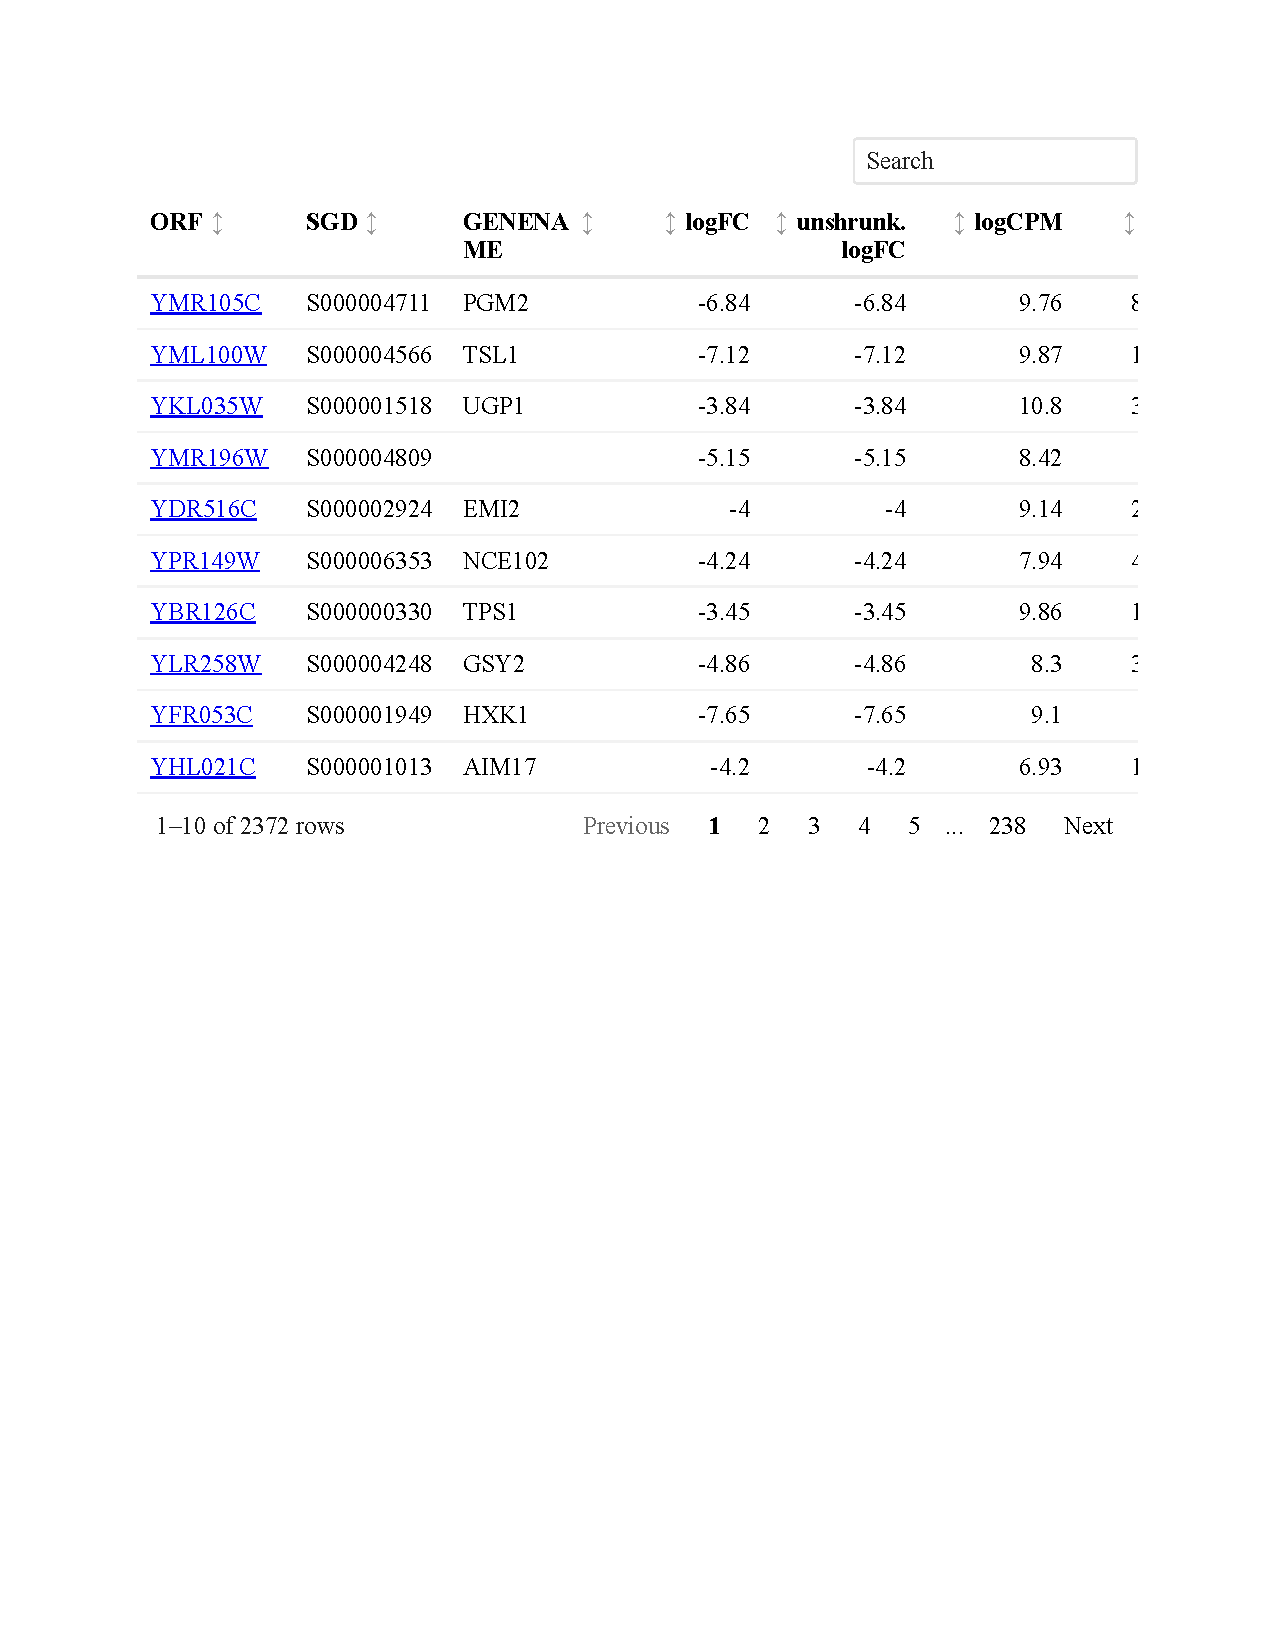
\includegraphics{_main_files/figure-latex/repeat-edgeRWorkflow-edgeR-1.pdf}

\begin{Shaded}
\begin{Highlighting}[]
\CommentTok{\# write the table to a tsv file}
\FunctionTok{topTags}\NormalTok{(tr, }\AttributeTok{n=}\ConstantTok{Inf}\NormalTok{) }\SpecialCharTok{|\textgreater{}} 
  \FunctionTok{data.frame}\NormalTok{() }\SpecialCharTok{|\textgreater{}} 
  \FunctionTok{arrange}\NormalTok{(FDR) }\SpecialCharTok{|\textgreater{}}
  \FunctionTok{mutate}\NormalTok{(}\AttributeTok{logFC=}\FunctionTok{round}\NormalTok{(logFC,}\DecValTok{2}\NormalTok{)) }\SpecialCharTok{|\textgreater{}}
  \CommentTok{\# mutate(across(where(is.numeric), signif, 3)) |\textgreater{}}
  \FunctionTok{mutate\_if}\NormalTok{(is.numeric, signif, }\DecValTok{3}\NormalTok{) }\SpecialCharTok{|\textgreater{}}
  \FunctionTok{write\_tsv}\NormalTok{(}\AttributeTok{x=}\NormalTok{\_, }\AttributeTok{file =} \FunctionTok{paste0}\NormalTok{(dir\_output\_edgeR, }\StringTok{"yeast\_lfc1topTags\_edgeR.tsv"}\NormalTok{))}

\CommentTok{\# summarize the DE genes}
\NormalTok{is.de\_tr }\OtherTok{\textless{}{-}} \FunctionTok{decideTestsDGE}\NormalTok{(tr, }\AttributeTok{p.value=}\FloatTok{0.05}\NormalTok{)}
\FunctionTok{summary}\NormalTok{(is.de\_tr)}
\end{Highlighting}
\end{Shaded}

\begin{verbatim}
##        1*WT.unstressed -1*WT.EtOH -1*msn24dd.unstressed 1*msn24dd.EtOH
## Down                                                               106
## NotSig                                                            2255
## Up                                                                  11
\end{verbatim}

\begin{Shaded}
\begin{Highlighting}[]
\CommentTok{\# visualize results}
\FunctionTok{plotSmear}\NormalTok{(tr, }\AttributeTok{de.tags=}\FunctionTok{rownames}\NormalTok{(tr)[is.de\_tr}\SpecialCharTok{!=}\DecValTok{0}\NormalTok{])}
\FunctionTok{title}\NormalTok{(}\AttributeTok{main=}\StringTok{"DE genes using glmTreat with logFC cutoff"}\NormalTok{)}
\end{Highlighting}
\end{Shaded}

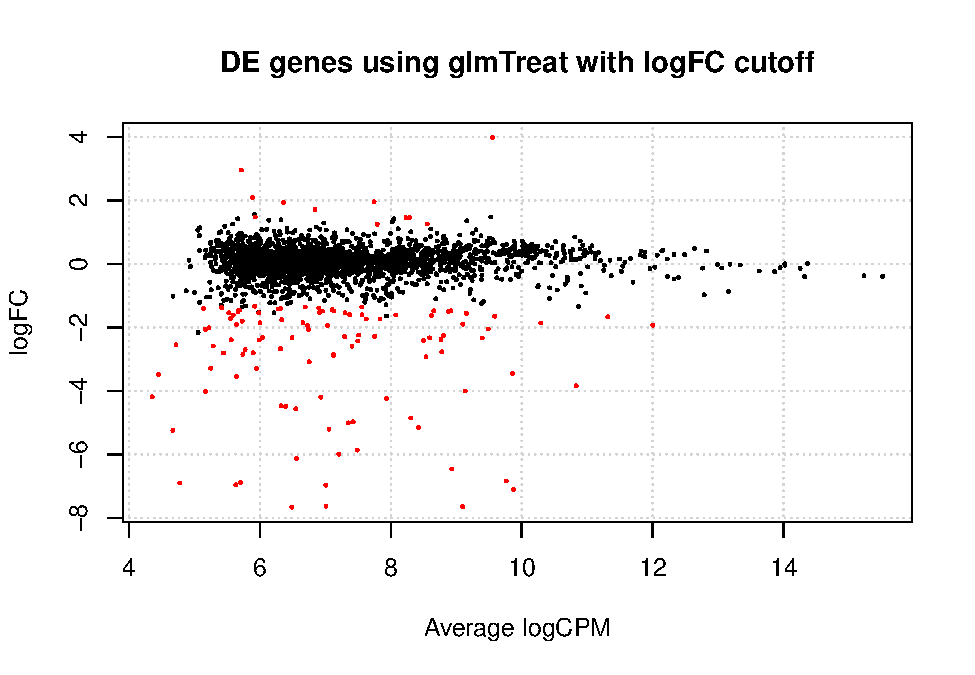
\includegraphics{_main_files/figure-latex/repeat-edgeRWorkflow-edgeR-2.pdf}

Be sure to knit this file into a pdf or html file once you're finished.

System information for reproducibility:

\begin{Shaded}
\begin{Highlighting}[]
\NormalTok{pander}\SpecialCharTok{::}\FunctionTok{pander}\NormalTok{(}\FunctionTok{sessionInfo}\NormalTok{())}
\end{Highlighting}
\end{Shaded}

\textbf{R version 4.3.1 (2023-06-16)}

\textbf{Platform:} aarch64-apple-darwin20 (64-bit)

\textbf{locale:}
en\_US.UTF-8\textbar\textbar en\_US.UTF-8\textbar\textbar en\_US.UTF-8\textbar\textbar C\textbar\textbar en\_US.UTF-8\textbar\textbar en\_US.UTF-8

\textbf{attached base packages:}
\emph{stats4}, \emph{stats}, \emph{graphics}, \emph{grDevices}, \emph{utils}, \emph{datasets}, \emph{methods} and \emph{base}

\textbf{other attached packages:}
\emph{edgeR(v.3.42.4)}, \emph{limma(v.3.56.2)}, \emph{reactable(v.0.4.4)}, \emph{webshot2(v.0.1.1)}, \emph{statmod(v.1.5.0)}, \emph{Rsubread(v.2.14.2)}, \emph{ShortRead(v.1.58.0)}, \emph{GenomicAlignments(v.1.36.0)}, \emph{SummarizedExperiment(v.1.30.2)}, \emph{MatrixGenerics(v.1.12.3)}, \emph{matrixStats(v.1.0.0)}, \emph{Rsamtools(v.2.16.0)}, \emph{GenomicRanges(v.1.52.1)}, \emph{Biostrings(v.2.68.1)}, \emph{GenomeInfoDb(v.1.36.4)}, \emph{XVector(v.0.40.0)}, \emph{BiocParallel(v.1.34.2)}, \emph{Rfastp(v.1.10.0)}, \emph{org.Sc.sgd.db(v.3.17.0)}, \emph{AnnotationDbi(v.1.62.2)}, \emph{IRanges(v.2.34.1)}, \emph{S4Vectors(v.0.38.2)}, \emph{Biobase(v.2.60.0)}, \emph{BiocGenerics(v.0.46.0)}, \emph{clusterProfiler(v.4.8.2)}, \emph{ggVennDiagram(v.1.2.3)}, \emph{tidytree(v.0.4.5)}, \emph{igraph(v.1.5.1)}, \emph{janitor(v.2.2.0)}, \emph{BiocManager(v.1.30.22)}, \emph{pander(v.0.6.5)}, \emph{knitr(v.1.44)}, \emph{here(v.1.0.1)}, \emph{lubridate(v.1.9.3)}, \emph{forcats(v.1.0.0)}, \emph{stringr(v.1.5.0)}, \emph{dplyr(v.1.1.3)}, \emph{purrr(v.1.0.2)}, \emph{readr(v.2.1.4)}, \emph{tidyr(v.1.3.0)}, \emph{tibble(v.3.2.1)}, \emph{ggplot2(v.3.4.4)}, \emph{tidyverse(v.2.0.0)} and \emph{pacman(v.0.5.1)}

\textbf{loaded via a namespace (and not attached):}
\emph{splines(v.4.3.1)}, \emph{later(v.1.3.1)}, \emph{bitops(v.1.0-7)}, \emph{ggplotify(v.0.1.2)}, \emph{polyclip(v.1.10-6)}, \emph{lifecycle(v.1.0.3)}, \emph{rprojroot(v.2.0.3)}, \emph{vroom(v.1.6.4)}, \emph{processx(v.3.8.2)}, \emph{lattice(v.0.21-9)}, \emph{MASS(v.7.3-60)}, \emph{crosstalk(v.1.2.0)}, \emph{magrittr(v.2.0.3)}, \emph{rmarkdown(v.2.25)}, \emph{yaml(v.2.3.7)}, \emph{cowplot(v.1.1.1)}, \emph{chromote(v.0.1.2)}, \emph{DBI(v.1.1.3)}, \emph{RColorBrewer(v.1.1-3)}, \emph{abind(v.1.4-5)}, \emph{zlibbioc(v.1.46.0)}, \emph{ggraph(v.2.1.0)}, \emph{RCurl(v.1.98-1.12)}, \emph{yulab.utils(v.0.1.0)}, \emph{tweenr(v.2.0.2)}, \emph{GenomeInfoDbData(v.1.2.10)}, \emph{enrichplot(v.1.20.0)}, \emph{ggrepel(v.0.9.4)}, \emph{codetools(v.0.2-19)}, \emph{DelayedArray(v.0.26.7)}, \emph{DOSE(v.3.26.1)}, \emph{ggforce(v.0.4.1)}, \emph{tidyselect(v.1.2.0)}, \emph{aplot(v.0.2.2)}, \emph{farver(v.2.1.1)}, \emph{viridis(v.0.6.4)}, \emph{webshot(v.0.5.5)}, \emph{jsonlite(v.1.8.7)}, \emph{ellipsis(v.0.3.2)}, \emph{tidygraph(v.1.2.3)}, \emph{tools(v.4.3.1)}, \emph{treeio(v.1.24.3)}, \emph{Rcpp(v.1.0.11)}, \emph{glue(v.1.6.2)}, \emph{gridExtra(v.2.3)}, \emph{xfun(v.0.40)}, \emph{qvalue(v.2.32.0)}, \emph{websocket(v.1.4.1)}, \emph{withr(v.2.5.1)}, \emph{fastmap(v.1.1.1)}, \emph{latticeExtra(v.0.6-30)}, \emph{fansi(v.1.0.5)}, \emph{digest(v.0.6.33)}, \emph{timechange(v.0.2.0)}, \emph{R6(v.2.5.1)}, \emph{gridGraphics(v.0.5-1)}, \emph{colorspace(v.2.1-0)}, \emph{GO.db(v.3.17.0)}, \emph{jpeg(v.0.1-10)}, \emph{RSQLite(v.2.3.1)}, \emph{utf8(v.1.2.3)}, \emph{generics(v.0.1.3)}, \emph{data.table(v.1.14.8)}, \emph{graphlayouts(v.1.0.1)}, \emph{httr(v.1.4.7)}, \emph{htmlwidgets(v.1.6.2)}, \emph{S4Arrays(v.1.0.6)}, \emph{scatterpie(v.0.2.1)}, \emph{pkgconfig(v.2.0.3)}, \emph{gtable(v.0.3.4)}, \emph{blob(v.1.2.4)}, \emph{hwriter(v.1.3.2.1)}, \emph{shadowtext(v.0.1.2)}, \emph{htmltools(v.0.5.6.1)}, \emph{bookdown(v.0.36)}, \emph{fgsea(v.1.26.0)}, \emph{scales(v.1.2.1)}, \emph{png(v.0.1-8)}, \emph{snakecase(v.0.11.1)}, \emph{ggfun(v.0.1.3)}, \emph{rstudioapi(v.0.15.0)}, \emph{tzdb(v.0.4.0)}, \emph{reshape2(v.1.4.4)}, \emph{rjson(v.0.2.21)}, \emph{nlme(v.3.1-163)}, \emph{cachem(v.1.0.8)}, \emph{RVenn(v.1.1.0)}, \emph{parallel(v.4.3.1)}, \emph{HDO.db(v.0.99.1)}, \emph{pillar(v.1.9.0)}, \emph{grid(v.4.3.1)}, \emph{vctrs(v.0.6.4)}, \emph{promises(v.1.2.1)}, \emph{archive(v.1.1.5)}, \emph{evaluate(v.0.22)}, \emph{cli(v.3.6.1)}, \emph{locfit(v.1.5-9.8)}, \emph{compiler(v.4.3.1)}, \emph{rlang(v.1.1.1)}, \emph{crayon(v.1.5.2)}, \emph{interp(v.1.1-4)}, \emph{reactR(v.0.5.0)}, \emph{ps(v.1.7.5)}, \emph{plyr(v.1.8.9)}, \emph{fs(v.1.6.3)}, \emph{stringi(v.1.7.12)}, \emph{viridisLite(v.0.4.2)}, \emph{deldir(v.1.0-9)}, \emph{munsell(v.0.5.0)}, \emph{lazyeval(v.0.2.2)}, \emph{GOSemSim(v.2.26.1)}, \emph{Matrix(v.1.6-1.1)}, \emph{hms(v.1.1.3)}, \emph{patchwork(v.1.1.3)}, \emph{bit64(v.4.0.5)}, \emph{KEGGREST(v.1.40.1)}, \emph{memoise(v.2.0.1)}, \emph{ggtree(v.3.8.2)}, \emph{fastmatch(v.1.1-4)}, \emph{bit(v.4.0.5)}, \emph{downloader(v.0.4)}, \emph{ape(v.5.7-1)} and \emph{gson(v.0.1.0)}

  \bibliography{book.bib,packages.bib}

\end{document}
